\chapter{Mass fit to \decay{\Bp}{\Dsp\Kp\Km} candidates} 
\label{ch:B2DsKK}

\minitoc

In this chapter the methodology used to search for \decay{\Bp}{\Dsp\Kp\Km} decays is described.
The branching fraction $\BF(\decay{\Bp}{\Dsp\Kp\Km})$ is determined by measuring the ratio of \decay{\Bp}{\Dsp\Kp\Km} and \decay{\Bp}{\Dsp\Dzb} yields. 
This ratio is corrected to account for the corresponding selection efficiencies of the two modes. Finally, the corrected yield ratio is multiplied by the externally measured branching fractions for the normalisation channel \decay{\Bp}{\Dsp\Dzb} and \decay{\Dzb}{\Kp\Km} decays to determine $\BF(\decay{\Bp}{\Dsp\Kp\Km})$.


% This is corrected by the ratio of efficiencies for the two modes and multiplied by the externally measured branching fractions for \decay{\Bp}{\Dsp\Dzb} and \decay{\Dzb}{\Kp\Km} decays.

% \begin{multline}
% \BF(\decay{\Bp}{\Dsp\Kp\Km}) = \frac{N(\decay{\Bp}{\Dsp\Kp\Km})}{N(\decay{\Bp}{\Dsp\Dzb})} \times  \frac{\epsilon(\decay{\Bp}{\Dsp\Dzb})}{\epsilon(\decay{\Bp}{\Dsp\Kp\Km})}\\ 
% \times \BF(\decay{\Bp}{\Dsp\Dzb}) \times \BF(\decay{\Dzb}{\Kp\Km}) 
% \end{multline}

The parametrisations used to model the signal and backgrounds components and extract the candidate yields are described in Section~\ref{sec:B2DsKK_fitcomps}, the efficiency corrections are described in Section~\ref{sec:B2DsKK_effcorrection} and the resulting calculation of the branching fraction is in Section~\ref{sec:B2DsKK_results}.



\section{Fit strategy}
\label{sec:B2DsKK_fitstrategy}
The search for $\decay{\Bp}{\Dsp\Kp\Km}$ involves two independent unbinned extended maximum likelihood fits for the signal and normalisation channels implemented with the \roofit package~\cite{Roofit} within \root. The extended likelihoods for the two fits are constructed in a similar manner to those already detailed in Sec.~\ref{sec:MVAbackgroundsubtraction}. However, as a larger number of components are included there are correspondingly more contributions included in the likelihood
\begin{equation}
-\log\mathcal{L}(n_{0}...n_{j},\vec{p}) = -\sum_{i}^{N} \log \left( \sum_{j} n_{j} f_{j}(m=m_{i},\vec{p}) \right) + \sum_{j}n_{j},
\end{equation}
where the index $j$ represents each component of the model with yield $n_{j}$ and PDF $f_{j}$.
As before, the PDF parameters are denoted by $\vec{p}$, the total number of events by $N$, the invariant mass variable by $m$, and the invariant mass of the $i$th candidate by $m_{i}$.
The constant $\log{N!}$ term has been ignored. Separate likelihoods are created for the signal and normalisation fits.



The raw $\decay{\Bp}{\Dsp\Kp\Km}$ yield is corrected on a per-candidate basis to account for the phase-space dependence of the signal efficiencies in this three-body decay. This is implemented using the \sPlot technique~\cite{Pivk:2004ty} to determine a signal weight $W_{\text{s},i}$ for each event $i$ in the fitted data set. The weights for each component are constructed such that they sum to the fitted value of that components yield
\begin{equation}
n_{\text{sig}} = \sum_{i}^{N} W_{\text{sig},i},
\end{equation}
where $n_{\text{sig}}$ is the fitted signal yield and $N$ is the total number of entries in the data set.
The efficiencies for the \decay{\Bp}{\Dsp\Kp\Km} signal decays are determined as a function of the kinematic properties of the decay. The weight for each entry $i$ in the data set is corrected with the appropriate efficiency for its given kinematics
\begin{equation}
n_{\text{sig},\text{corr}} = \sum_{i}^{N} \frac{W_{\text{sig},i}}{\epsilon_{i}}.
\label{eq:B2DsKK_corrected_yield}
\end{equation}
The propagation of the uncertainty in this corrected yields is described in Sec.~\ref{sec:B2DsKK_results}.

The normalisation channel decay proceeds via a pseudo two-body process, therefore no kinematic dependent efficiency correction is required.  



\section{Fit components}
\label{sec:B2DsKK_fitcomps}

In order to extract the yields of \decay{\Bp}{\Dsp\Dzb} and \decay{\Bp}{\Dsp\Kp\Km} decays the invariant mass distributions for the processes contributing within the invariant mass range are parametrised with probability density functions (PDFs).
Both the signal and normalisation channels are considered within the same \Bp meson invariant mass range 5100--5900\mevcc. This is sufficiently wide to allow the contributions from different background components to be distinguished and accurately extrapolated into the signal region. The entire $m(\Kp\Km)$ phase-space is included in the search for the signal decays, including the range in the vicinity of the \phiz meson used later in Chapter~\ref{ch:B2DsPhi}. 



\subsection{Signal and normalisation decays}
\label{sec:B2DsKK_sigcomps}

The invariant mass distributions of \decay{\Bp}{\Dsp\Dzb} and \decay{\Bp}{\Dsp\Kp\Km} decays are parametrised as the sum of two Crystal Ball (CB) functions.
The CB function consists of a Gaussian function with a power-law tail and is typically used to parametrise losses due to radiative processes.
This is defined as
\begin{equation}
\text{CB}(m|\mu,\sigma,n,\alpha) = \left \{
  \begin{aligned}
    &e^{-\frac{1}{2} \left(\frac{m-\mu}{\sigma}\right)^2}, && \text{if}\ \left(\frac{m-\mu}{\sigma}\right) < -|\alpha|\\
    &\frac{\left(\frac{n}{|\alpha|}\right)^n\times e ^{-\frac{1}{2}|\alpha|^2} }{\left(\frac{n}{|\alpha|}-|\alpha| - \frac{m-\mu}{\sigma}\right)^n}, && \text{otherwise}
  \end{aligned} \right.
\end{equation} 

where $\mu$, $\sigma$, $n$ and $\alpha$ are adjustable parameters and $m$ is the \B meson invariant mass observable.
The sum of two CB functions is constructed with a variable fraction $f_\sigma$ assigned to the CB function with the narrower width,
\begin{equation}
\text{DCB}(m|\mu,\sigma_1,\sigma_2,n,\alpha) = f_\sigma \times \text{CB}(m|\mu,\sigma_1,n,\alpha) + (1-f_\sigma) \times \text{CB}(m|\mu,\sigma_2,n,\alpha),
\label{eq:DoubleBD}
\end{equation}
where the same tail parameters, $n$ and $\alpha$ are used for both functions, but the widths, $\sigma_1$ and $\sigma_2$, are allowed to be different (with $\sigma_1 < \sigma_2$).
As both CB shapes have the same parameter $\alpha$, the tails are constrained to be on the same side.
Values for the adjustable parameters are determined from fits to simulated decays passing the selection requirements applied to the data. 
%These are determined separately for the different \Dsp decay modes. 
However, a number of parameters are not completely constrained from the simulations. The mean position $\mu$ is allowed vary freely in the fit to data, as is the narrowest CB width of the normalisation and signal decays. 
%The ratios $\sigma_1/\sigma_2$ and $\sigma_{1}(\Dsp\phi) / \sigma_{1}(\Dsp\Dzb)$ are fixed from simulations.
The tail parameters $n$ and $\alpha$ are highly correlated, therefore the value of $n$ is fixed to unity in both the fits to simulations and data. 
The simulation invariant mass fits and corresponding fixed values are detailed in Appendix.~\ref{sec:appendix_MCfits_B2DsKK}. 
%The values determined from simulations for \decay{\Bp}{\Dsp\Dzb} and \decay{\Bp}{\Dsp\Kp\Km} decays are tabulated in Table~\ref{tab:B2DsKK_signal_mc_fits} and the results of the corresponding fits are shown in Fig.~\ref{fig:B2DsKK_signal_fits}.


% %%%%%%%%%%%%%%%%%%%%%%%%%%%%%%%%%%%%%%%%%%%%%%%%%%%%%%%%%% 
% \begin{table}[h]
% \centering 
% \begin{tabular}{ c c }
% \hline
% Parameter                   & Value \\
% \hline
% \multicolumn{2}{c} {\decay{\Bp}{\Dsp\Kp\Km}}\\

% \hline
% $\sigma_1/\sigma_2$         & 0.53 $\pm$ 0.02  \\
% $f_\sigma$                  & 0.87 $\pm$ 0.02  \\
% $\alpha$                    & 2.60 $\pm$ 0.03  \\
% $n$                         & 1 $\pm$ 0        \\
% \hline
% \multicolumn{2}{c} {\decay{\Bp}{\Dsp\Dzb}}\\
% \hline
% $\sigma_1/\sigma_2$         & 0.60 $\pm$ 0.03    \\
% $f_\sigma$                  & 0.66 $\pm$ 0.12    \\
% $\alpha$                    & 2.67 $\pm$ 0.12    \\
% $n$                         & 1 $\pm$ 0          \\
% \hline
% \end{tabular} 
% \caption{Fixed values obtained in fits to simulations used in the model for the signal and normalisation PDFs. The uncertainties are determined in the fits to simulated decays. The uncertainties used to extract the systematic uncertainty arising from the finite simulation sizes.} 
% \label{tab:B2DsKK_signal_mc_fits}
% \end{table}
% %%%%%%%%%%%%%%%%%%%%%%%%%%%%%%%%%%%%%%%%%%%%%%%%%%%%%%%%%% 

% %%%%%%%%%%%%%%%%%%%%%%%%%%%%%%%%%%%%%%%%%%%%%%%%%%%%%%%%%%
% \begin{figure}[!h]
%     \centering
%     \begin{subfigure}[t]{1.0\textwidth}
%         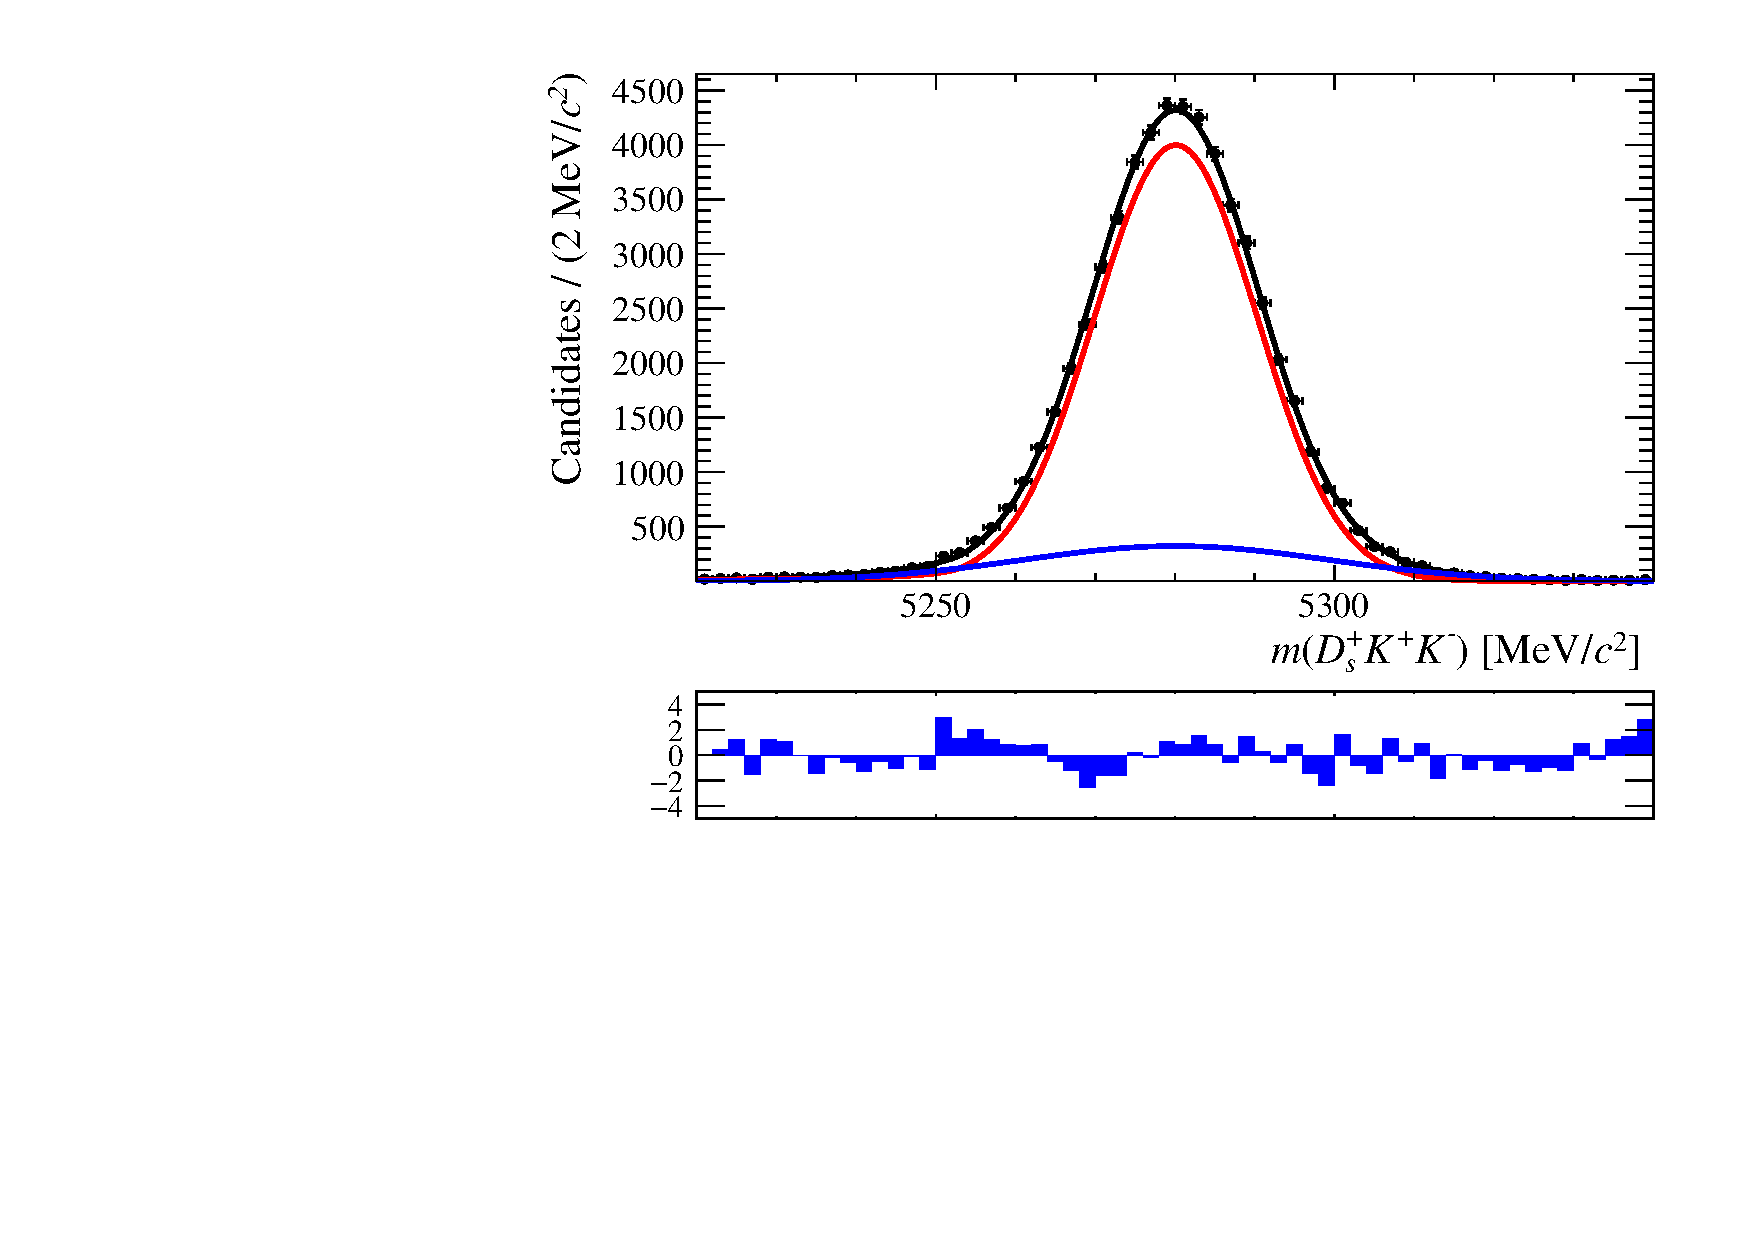
\includegraphics[width=0.48\textwidth]{figs/B2DsKK/Plot_Signal_Fit_All_B2DsKK_Ds2KKPi.pdf}
%         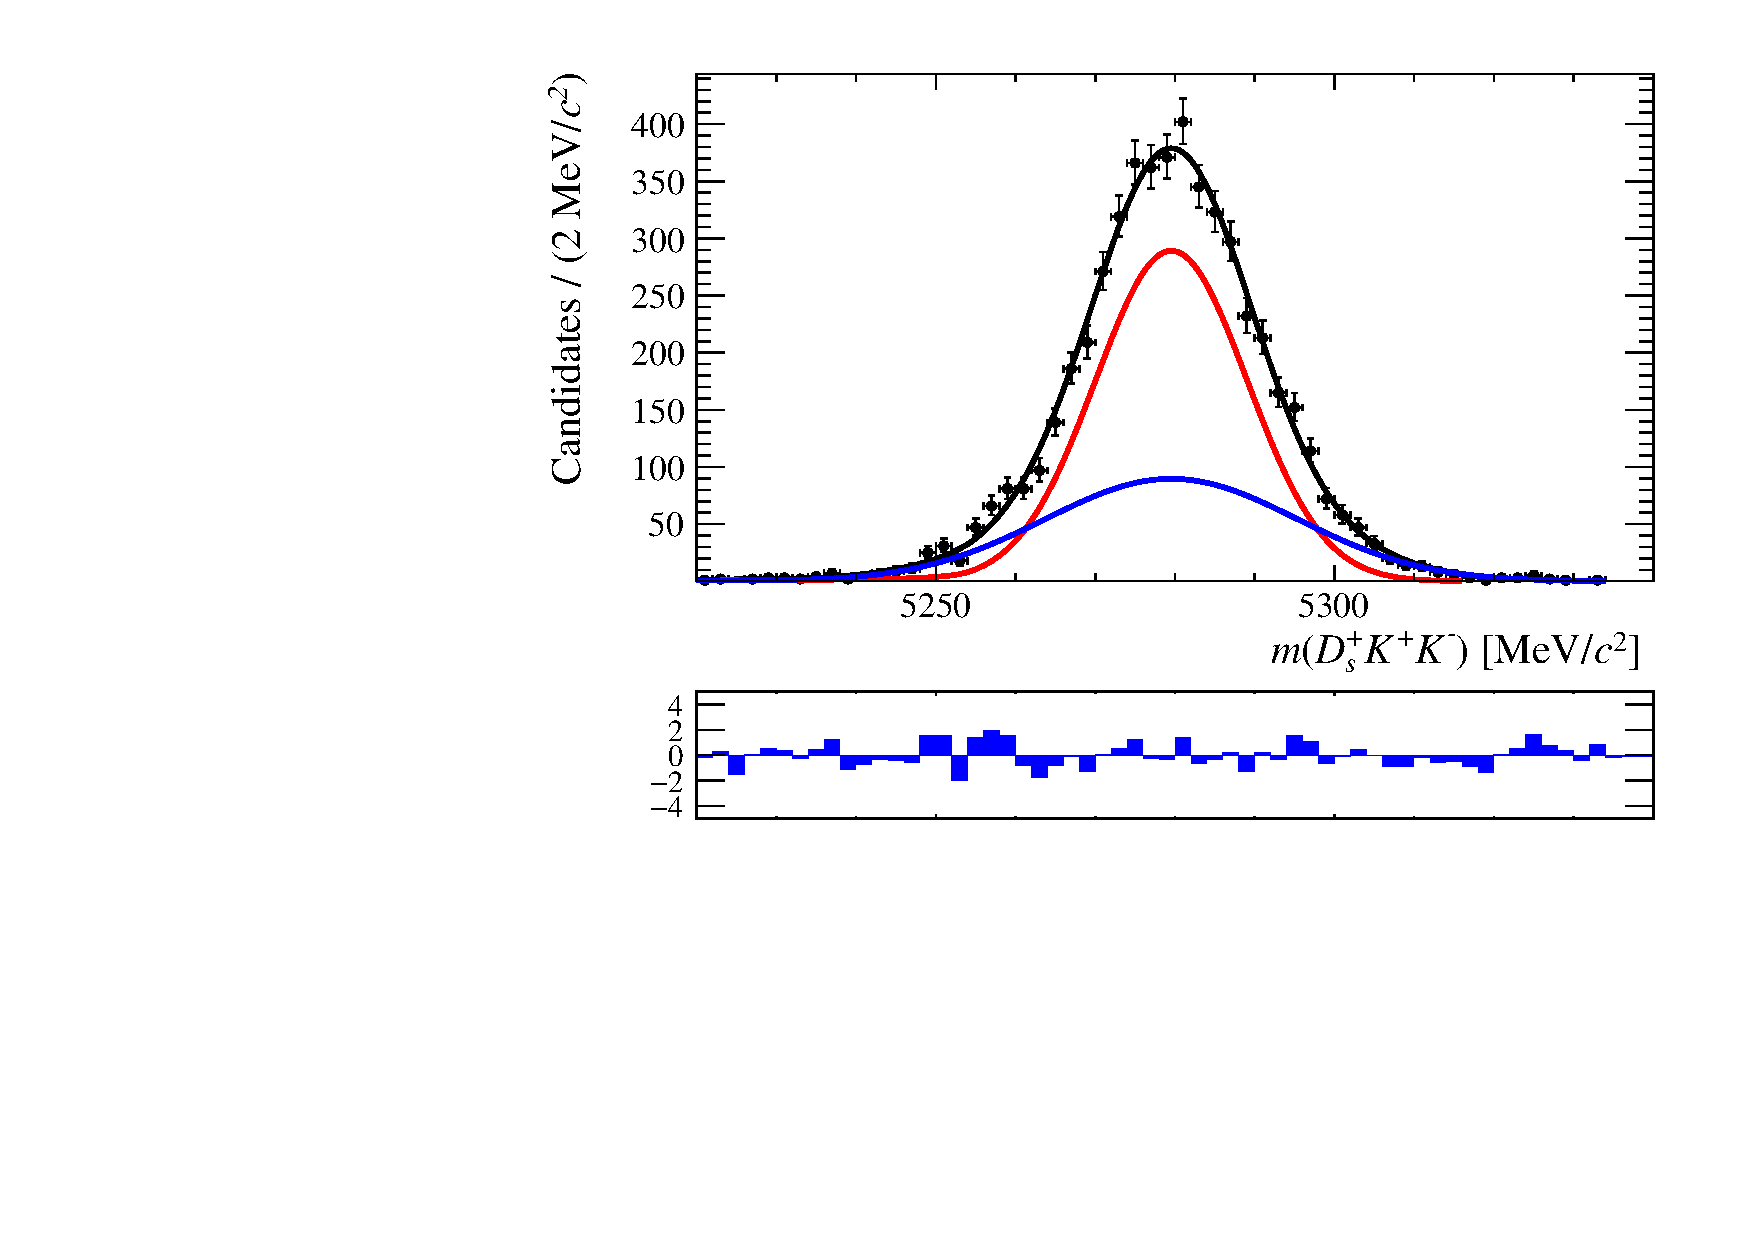
\includegraphics[width=0.48\textwidth]{figs/B2DsKK/Plot_Signal_Fit_All_B2DsD0_Ds2KKPi.pdf}
%     \end{subfigure}\\
%     \caption{Invariant mass fits to signal (left) and normalisation (right) channel simulation samples.}
%     \label{fig:B2DsKK_signal_fits}   
% \end{figure}
% %%%%%%%%%%%%%%%%%%%%%%%%%%%%%%%%%%%%%%%%%%%%%%%%%%%%%%%%%%


\subsection{Partially reconstructed backgrounds}
\label{sec:B2DsKK_partrecocomps}

Partially reconstructed decays are those in which the five final state particles combined in the signal mode are only a subset of a background mode's final state.
Decays of \bquark-hadrons can contribute at lower invariant masses below the signal peak when one or more the decay products have not been reconstructed. 
For decays to contribute within the fitted \Bp invariant mass window, the particle or particles that have not been reconstructed must be fairly low-momentum (soft) such that the invariant mass of the remaining particles is large. Accurate parametrisation of these contributions is vital as many of the distributions extend close to or within the range of the signal distribution. Incorrectly attributing these decays to the signal component could lead to the incorrect branching fraction being measured. 

\subsubsection{Backgrounds to the normalisation channel, \decay{\Bp}{\Dsp\Dzb}}
\label{sec:B2DsKK_norm_partreco}

The low invariant mass region of the \Dsp\Dzb spectrum is populated by decays of \Bp mesons to combinations of \D and excited \D mesons. These \Dstarzb and \Dss mesons decay strongly to a ground state \Dzb or \Dsp meson and a soft pion or photon. The branching fractions for these decays are listed in Table~\ref{tab:dstar_BFs}.


%%%%%%%%%%%%%%%%%%%%%%%%%%%%%%%%%%%%%%%%%%%%%%%%%%%%%%%%%% 
\begin{table}[h]
\centering
\begin{tabular}{ l c }

\hline
Decay                           & Branching fraction \\ 
\hline
\decay{\Dstarzb}{\Dzb\Pgamma}   &   $(64.7\pm0.9)\%$ \\
\decay{\Dstarzb}{\Dzb\piz}      &   $(35.3\pm0.9)\%$ \\
\decay{\Dssp}{\Dsp\Pgamma}      &   $(93.5\pm0.7)\%$ \\
\decay{\Dssp}{\Dsp\piz}         &    $(5.8\pm0.7)\%$ \\
\hline

\end{tabular}  
\caption{Branching fractions for excited charm mesons \cite{PDG2016}. } 
\label{tab:dstar_BFs}
\end{table}
%%%%%%%%%%%%%%%%%%%%%%%%%%%%%%%%%%%%%%%%%%%%%%%%%%%%%%%%%% 
The excited charm mesons \Dstarzb and \Dss are vector ($J^{P} = 1^{-}$) mesons. The partially reconstructed invariant mass of the \Dsp and \Dzb mesons, $m(\Dsp\Dzb)$, varies depending on the angle at which the missing particle was produced, as shown in Fig.~\ref{fig:B2DsKK_partreco_decay}. The distribution of this angle depends on the spin of the missing particle. 
Analytical PDFs are used to account for the spin and mass of the missing particle. These PDFs have been used to describe other partially reconstructed \decay{\B}{\D X} decays investigated by the LHCb collaboration~\cite{LHCb-PAPER-2017-021}. 

%%%%%%%%%%%%%%%%%%%%%%%%%%%%%%%%%%%%%%%%%%%%%%%%%%%%%%%%%%
\begin{figure}[!h]
    \centering
    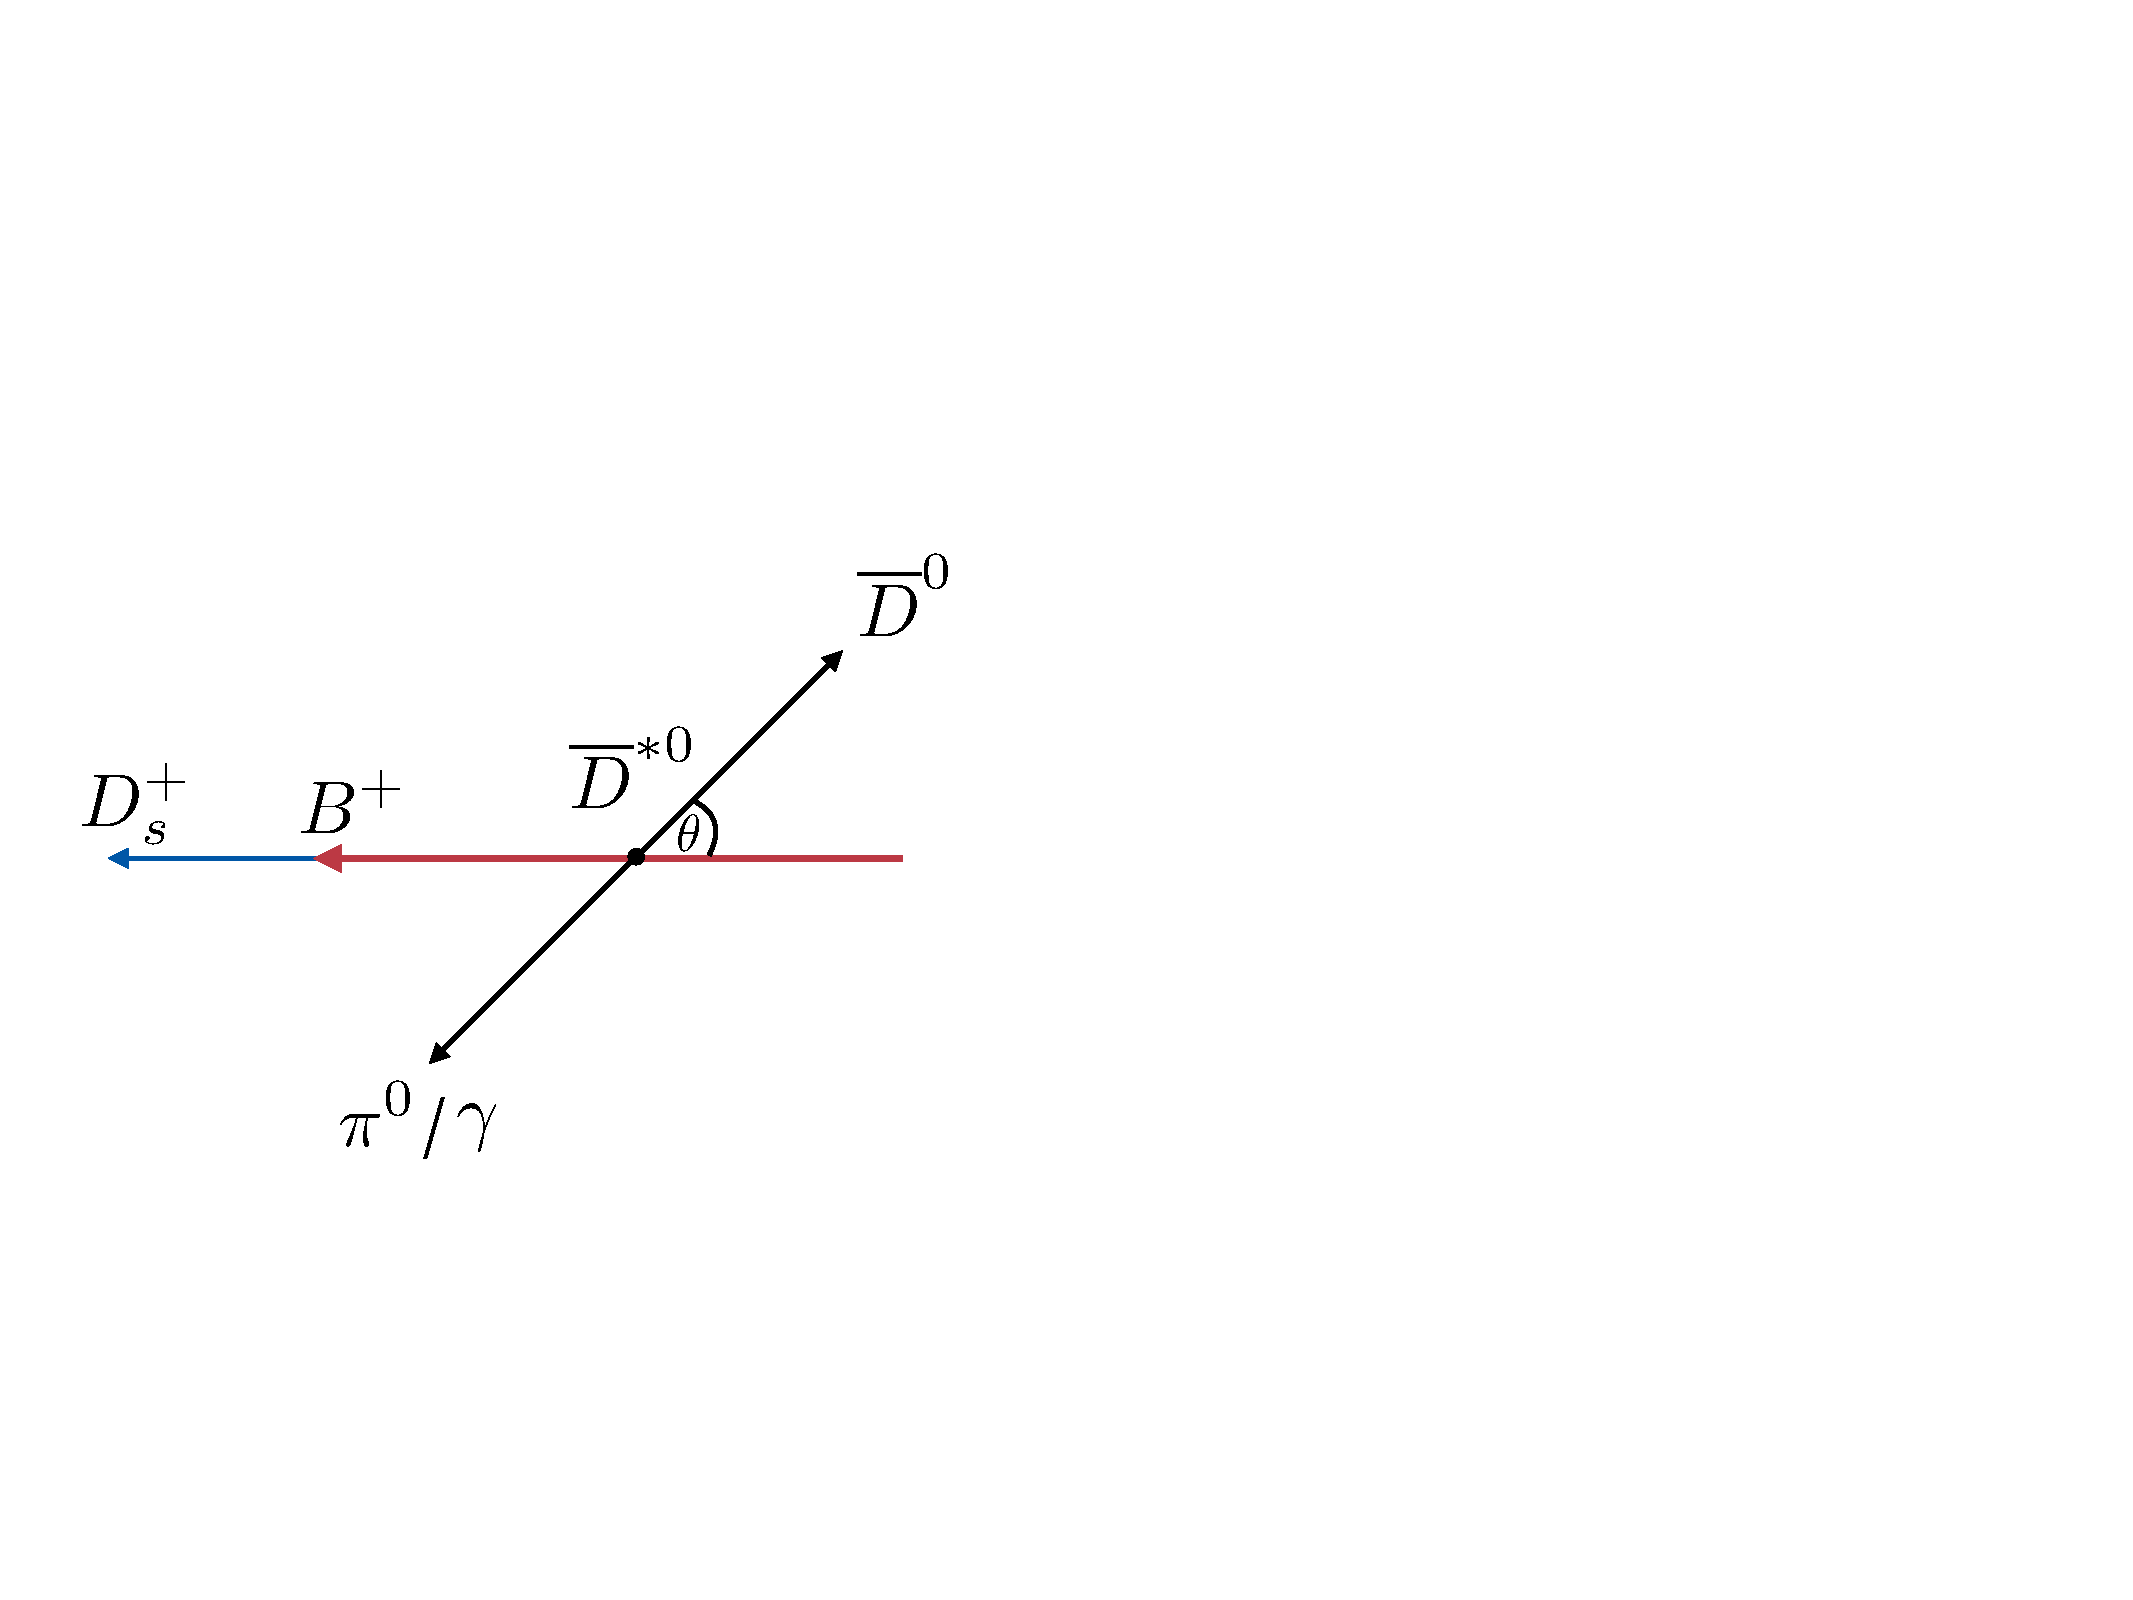
\includegraphics[width=0.5\textwidth]{figs/B2DsKK/partreco_decay.pdf}
    \caption{The \decay{\Bp}{\Dsp(\decay{\Dstarzb}{\Dzb \piz/\Pgamma})} decay in the \Dstarzb rest frame. The invariant mass $m(\Dsp\Dzb)$ is highest when $\theta = 0\degrees$ and lowest when $\theta = 180\degrees$. Spin-0 particles (\piz) are emitted preferentially at angles $\theta = 0, 180\degrees$, leading to an invariant mass distribution with two peaks at high and low $m(\Dsp\Dzb)$. Spin-1 particles (\Pgamma) are emitted preferentially at angles $\theta = 90,270\degrees$, both of which correspond to intermediate $m(\Dsp\Dzb)$, resulting in a singly peaked distribution.} 
    \label{fig:B2DsKK_partreco_decay}   
\end{figure}
%%%%%%%%%%%%%%%%%%%%%%%%%%%%%%%%%%%%%%%%%%%%%%%%%%%%%%%%%%


\begin{description}
\item \textbf{\decay{\Bp}{(\decay{\Dssp}{\Dsp[\piz]})\Dzb} and \decay{\Bp}{\Dsp(\decay{\Dstarzb}{\Dzb[\piz]})}:} the \piz meson is a pseudo-scalar ($J^{P} = 0^{-}$) particle with a mass $m(\piz) = 134.9766 \pm 0.0006 \mevcc$. The partially reconstructed invariant mass distribution $m(\Dsp\Dzb)$ can be described by a parabola convolved with a Gaussian resolution function as pictorially represented in Fig.~\ref{fig:B2DsKK_partreco_diagram}. The parabola does not extend beyond kinematic endpoints, $a$ and $b$, that arise from the relative direction of the missing particle (Fig.~\ref{fig:B2DsKK_partreco_decay}). The parabola has a minimum in the centre 
\begin{equation}
f(m|a,b,\sigma,\xi, \delta) = \int_{a}^{b}\left(\mu-\frac{a+b}{2}\right)^{2} \left( \frac{1-\xi}{b-a}\mu + \frac{b\xi-a}{b-a} \right) e^{-\frac{-(\mu-(m-\delta))^{2}}{2\sigma^{2}}} d\mu.
\label{eq:DsPhi_RooHorns}
\end{equation} 

Here, $\sigma$ is the width of the resolution Gaussian and $\delta$ allows the function to be offset in invariant mass, accounting for any differences in the reconstructed and predicted kinematic endpoints. The parameter $\xi$ introduces the freedom for the two sides of the parabola to have difference heights, achieved by multiplying the parabola by a line whose slope is depends on $\xi$. This accounts for variation in the selection efficiency across the PDF. The resulting function is a double peaked structure shown in Fig.~\ref{fig:B2DsKK_DsD0_partreco}.   
The parameters $a$ and $b$ are calculated from the kinematics of the \decay{\Bp}{(\decay{\Dssp}{\Dsp\piz})\Dzb} and \decay{\Bp}{\Dsp(\decay{\Dstarzb}{\Dzb\piz})} decays respectively, and are listed in Table~\ref{tab:DsKK_pi0_a_and_b}.

\end{description}



%%%%%%%%%%%%%%%%%%%%%%%%%%%%%%%%%%%%%%%%%%%%%%%%%%%%%%%%%%
\begin{figure}[!h]
    \centering
    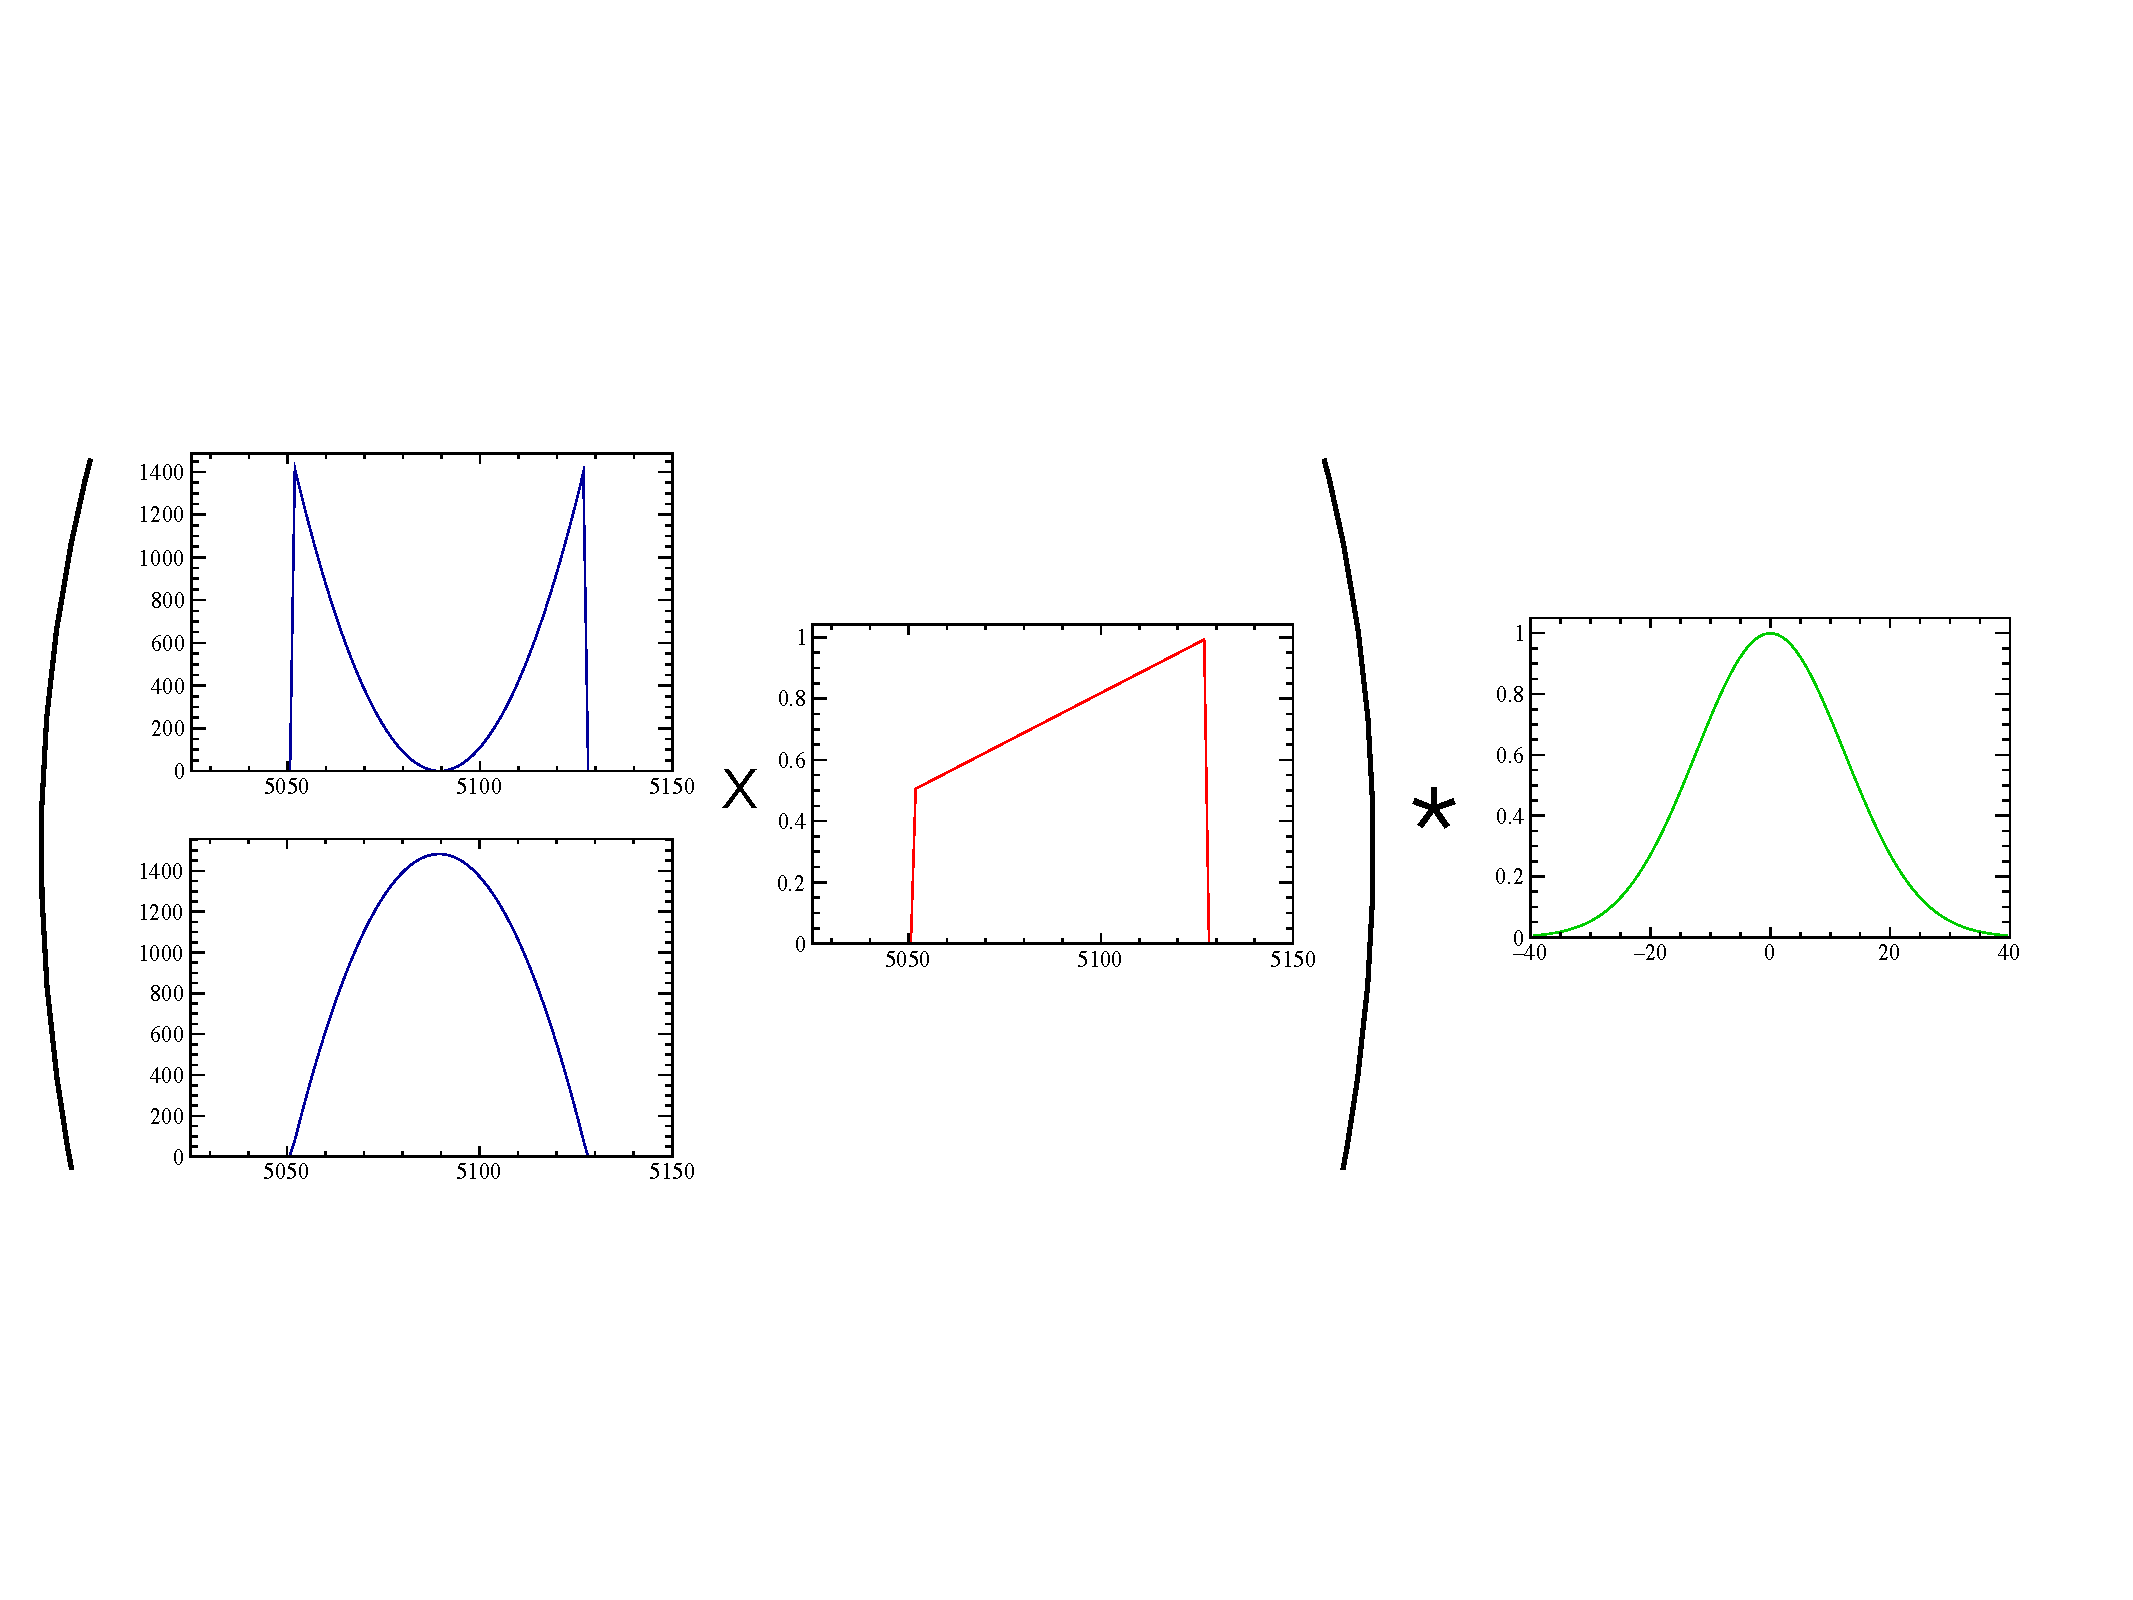
\includegraphics[width=1.0\textwidth]{figs/B2DsKK/partreco_diagram.pdf}
    \caption{Components of the analytical PDFs used to represent various partially reconstructed \decay{\B}{\D X} decays. Parabolas determined by the spin of the missing particle are shown in blue and the linear function used to account for the relative selection efficiency is shown in red. The product of these are convolved with a Gaussian resolution function, shown in green.} 
    \label{fig:B2DsKK_partreco_diagram}   
\end{figure}
%%%%%%%%%%%%%%%%%%%%%%%%%%%%%%%%%%%%%%%%%%%%%%%%%%%%%%%%%%



\begin{description}

%%%%%%%%%%%%%%%%%%%%%%%%%%%%%%%%%%%%%%%%%%%%%%%%%%%%%%%%%% 
\begin{table}[h]
\centering
\begin{tabular}{ l c c }

\hline
Mode                                              & $a$ (\mevcc)       & $b$ (\mevcc)   \\ 
\hline
\decay{\Bp}{(\decay{\Dssp}{\Dsp[\piz]})\Dzb}      & 5051.4            &  5132.9       \\
\decay{\Bp}{\Dsp(\decay{\Dstarzb}{\Dzb[\piz]})}   & 5051.5            &  5128.6       \\
\hline
\end{tabular}  
\caption{Kinematic endpoints for the partially reconstructed \decay{\Bp}{(\decay{\Dssp}{\Dsp\piz})\Dzb} and \decay{\Bp}{\Dsp(\decay{\Dstarzb}{\Dzb\piz})} decays.} 
\label{tab:DsKK_pi0_a_and_b}
\end{table}
%%%%%%%%%%%%%%%%%%%%%%%%%%%%%%%%%%%%%%%%%%%%%%%%%%%%%%%%%%


\item \textbf{\decay{\Bp}{(\decay{\Dssp}{\Dsp[\Pgamma]})\Dzb} and \decay{\Bp}{\Dsp(\decay{\Dstarzb}{\Dzb[\Pgamma]})}:} the \Pgamma boson is a massless vector ($J^{P} = 1^{-}$) particle. The partially reconstructed $m(\Dsp\Dzb)$ invariant mass is also described by a parabola convolved with a Gaussian resolution function. The parabola does not extend beyond the endpoints $a$ and $b$, and has a maximum in the centre   
\begin{equation}
f(m|a,b,\sigma,\xi, \delta) = \int_{a}^{b} -(\mu-a)(\mu-b)\left( \frac{1-\xi}{b-a}\mu + \frac{b\xi-a}{b-a} \right) e^{-\frac{-(\mu-(m-\delta))^{2}}{2\sigma^{2}}} d\mu.
\label{eq:DsPhi_RooHills}
\end{equation}
Again $\sigma$, $\delta$ and $\xi$ control the width, offset and relative heights of two sides of the parabola. The resulting function is a broad single peak shown in Fig.~\ref{fig:B2DsKK_DsD0_partreco}.

\end{description}

%%%%%%%%%%%%%%%%%%%%%%%%%%%%%%%%%%%%%%%%%%%%%%%%%%%%%%%%%% 
\begin{table}[h]
\centering
\begin{tabular}{ l c c }

\hline
Mode                                                 & $a$ (\mevcc)      & $b$ (\mevcc)  \\ 
\hline
\decay{\Bp}{(\decay{\Dssp}{\Dsp[\Pgamma]})\Dzb}      & 4976.7            &  5213.1       \\
\decay{\Bp}{\Dsp(\decay{\Dstarzb}{\Dzb[\Pgamma]})}   & 4970.1            &  5216.1       \\
\hline
\end{tabular}  
\caption{Kinematic endpoints for the partially reconstructed \decay{\Bp}{(\decay{\Dssp}{\Dsp\Pgamma})\Dzb} and \decay{\Bp}{\Dsp(\decay{\Dstarzb}{\Dzb\Pgamma})} decays.} 
\label{tab:DsKK_gamma_a_and_b}
\end{table}
%%%%%%%%%%%%%%%%%%%%%%%%%%%%%%%%%%%%%%%%%%%%%%%%%%%%%%%%%%


%%%%%%%%%%%%%%%%%%%%%%%%%%%%%%%%%%%%%%%%%%%%%%%%%%%%%%%%%%
\begin{figure}[!h]
    \centering
    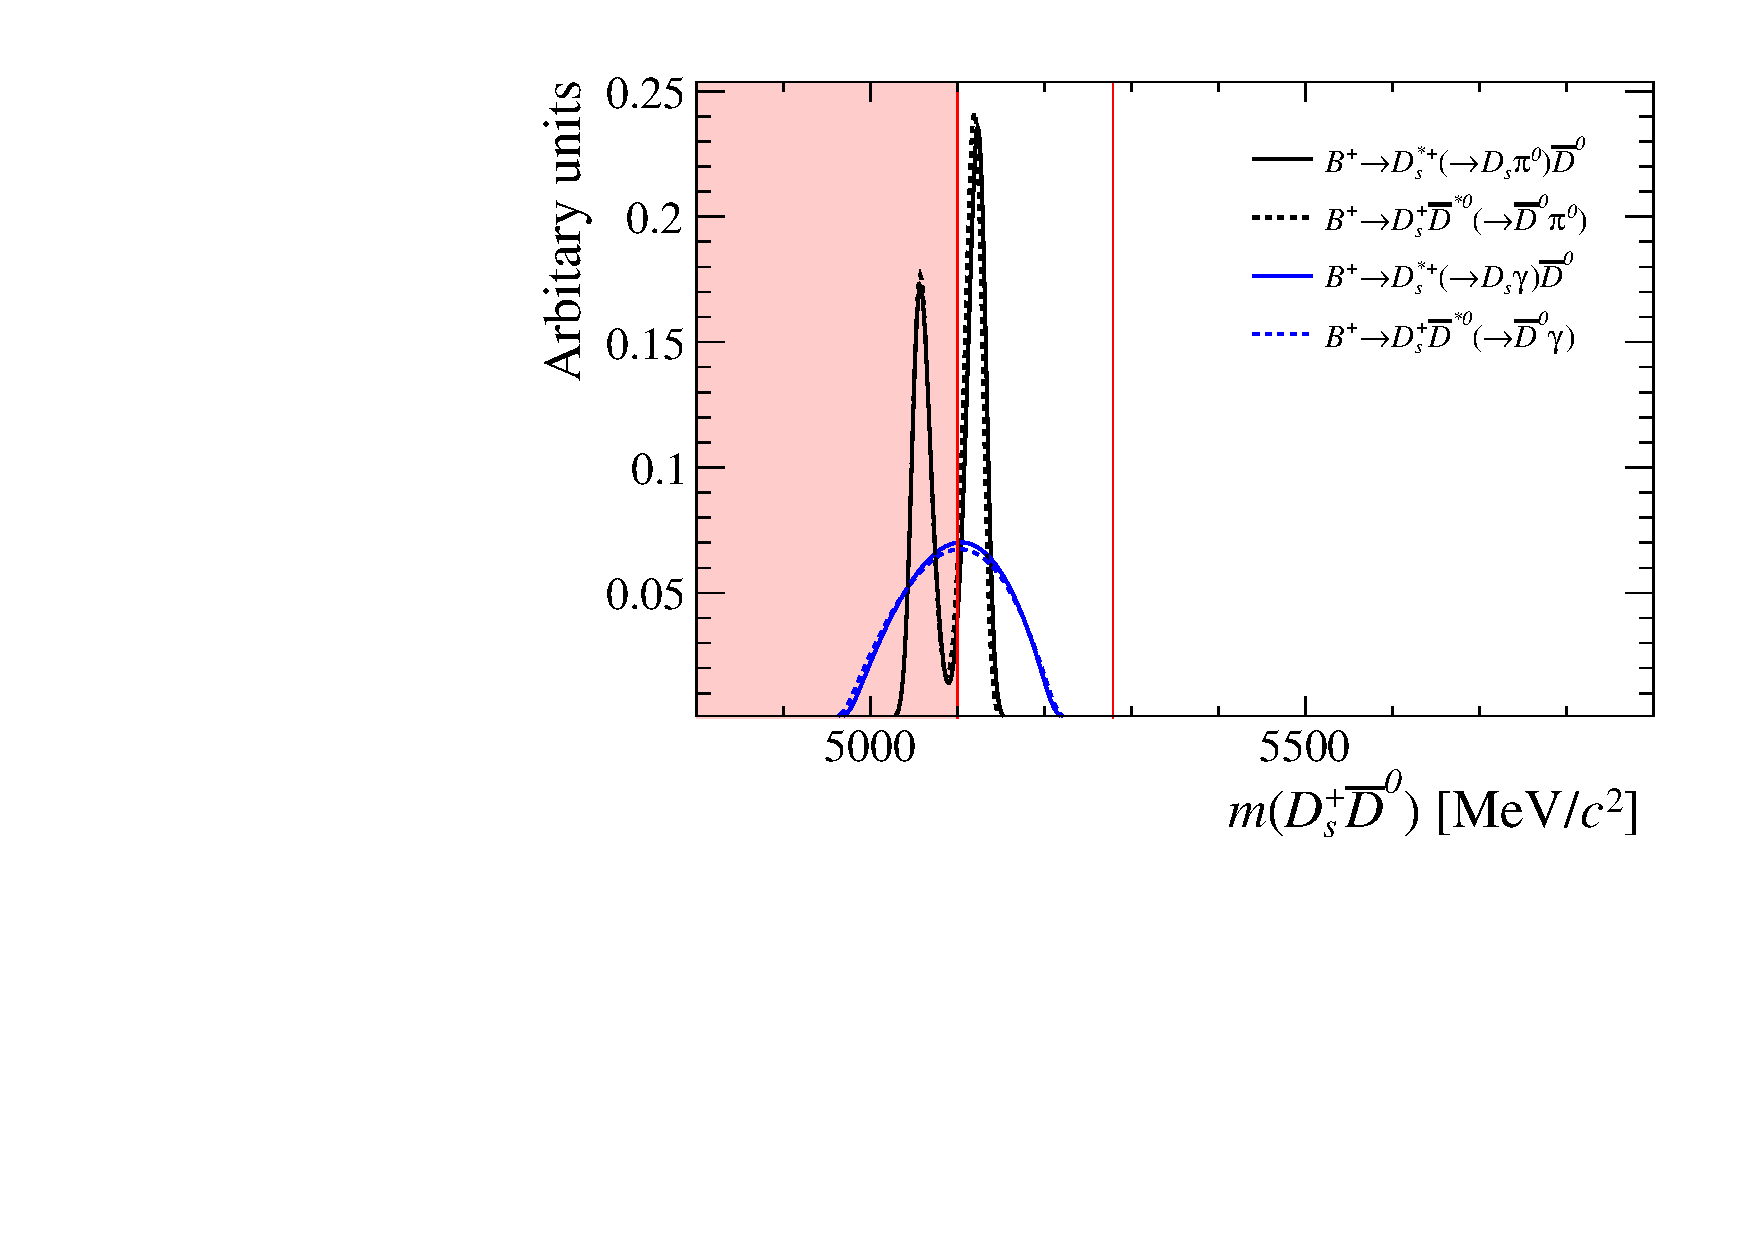
\includegraphics[width=0.80\textwidth]{figs/B2DsKK/B2DsKK_DsD0_part_reco_Shapes.pdf}
    \caption{Partially reconstructed \decay{\Bp}{\Dssp\Dzb} and \decay{\Bp}{\Dsp\Dstarzb} PDFs as described in Sec.~\ref{sec:B2DsKK_norm_partreco}. The range below $5100\mevcc$ (highlighted in red) is not included in the fit range, but included to shown the full PDF distributions. The \Bp meson mass is represented by a vertical line.} 
    \label{fig:B2DsKK_DsD0_partreco}   
\end{figure}
%%%%%%%%%%%%%%%%%%%%%%%%%%%%%%%%%%%%%%%%%%%%%%%%%%%%%%%%%%





\subsubsection{Backgrounds to the signal channel, \decay{\Bp}{\Dsp\Kp\Km}}
\label{sec:B2DsKK_sig_partreco}
The signal channel receives contributions at low invariant mass from a number of different decays. 
All modes considered involve a \Bs or \Bz meson decay in which one or more soft decay products have not been reconstructed.
Decays of \Bs mesons are particularly dominant as the \Bs meson has a larger mass than the \Bp meson.   

\begin{description}
\item \decay{\Bsb}{\Dsp\Km\Kstarz}: this decay can form a background to the \decay{\Bp}{\Dsp\Kp\Km} signal when a pion from the \decay{\Kstarz}{\Kp\pim} decay is not reconstructed. The $\Km\Kstarz$ is modelled as originating from the $a_1(1260)$ resonance. This resonance has a width of 250--600\mevcc~\cite{PDG2016}, allowing it to decay to $\Km\Kstarz$ even though it's pole mass is below the $\Km\Kstarz$ threshold.
The PDF for this background is determined from a sample of fully reconstructed simulated events that have been processed using the same procedure as the signal decays. The PDF is created using a kernel estimation technique~\cite{Cranmer:2000du} implemented in the \texttt{RooKeysPDF} class within \roofit. The resulting PDF is shown in Fig.~\ref{fig:B2DsKK_part_reco_backgrounds_DsKKstar}.
\end{description}

%%%%%%%%%%%%%%%%%%%%%%%%%%%%%%%%%%%%%%%%%%%%%%%%%%%%%%%%%%
\begin{figure}[!h]
    \centering
    \begin{subfigure}[t]{0.49\textwidth}
        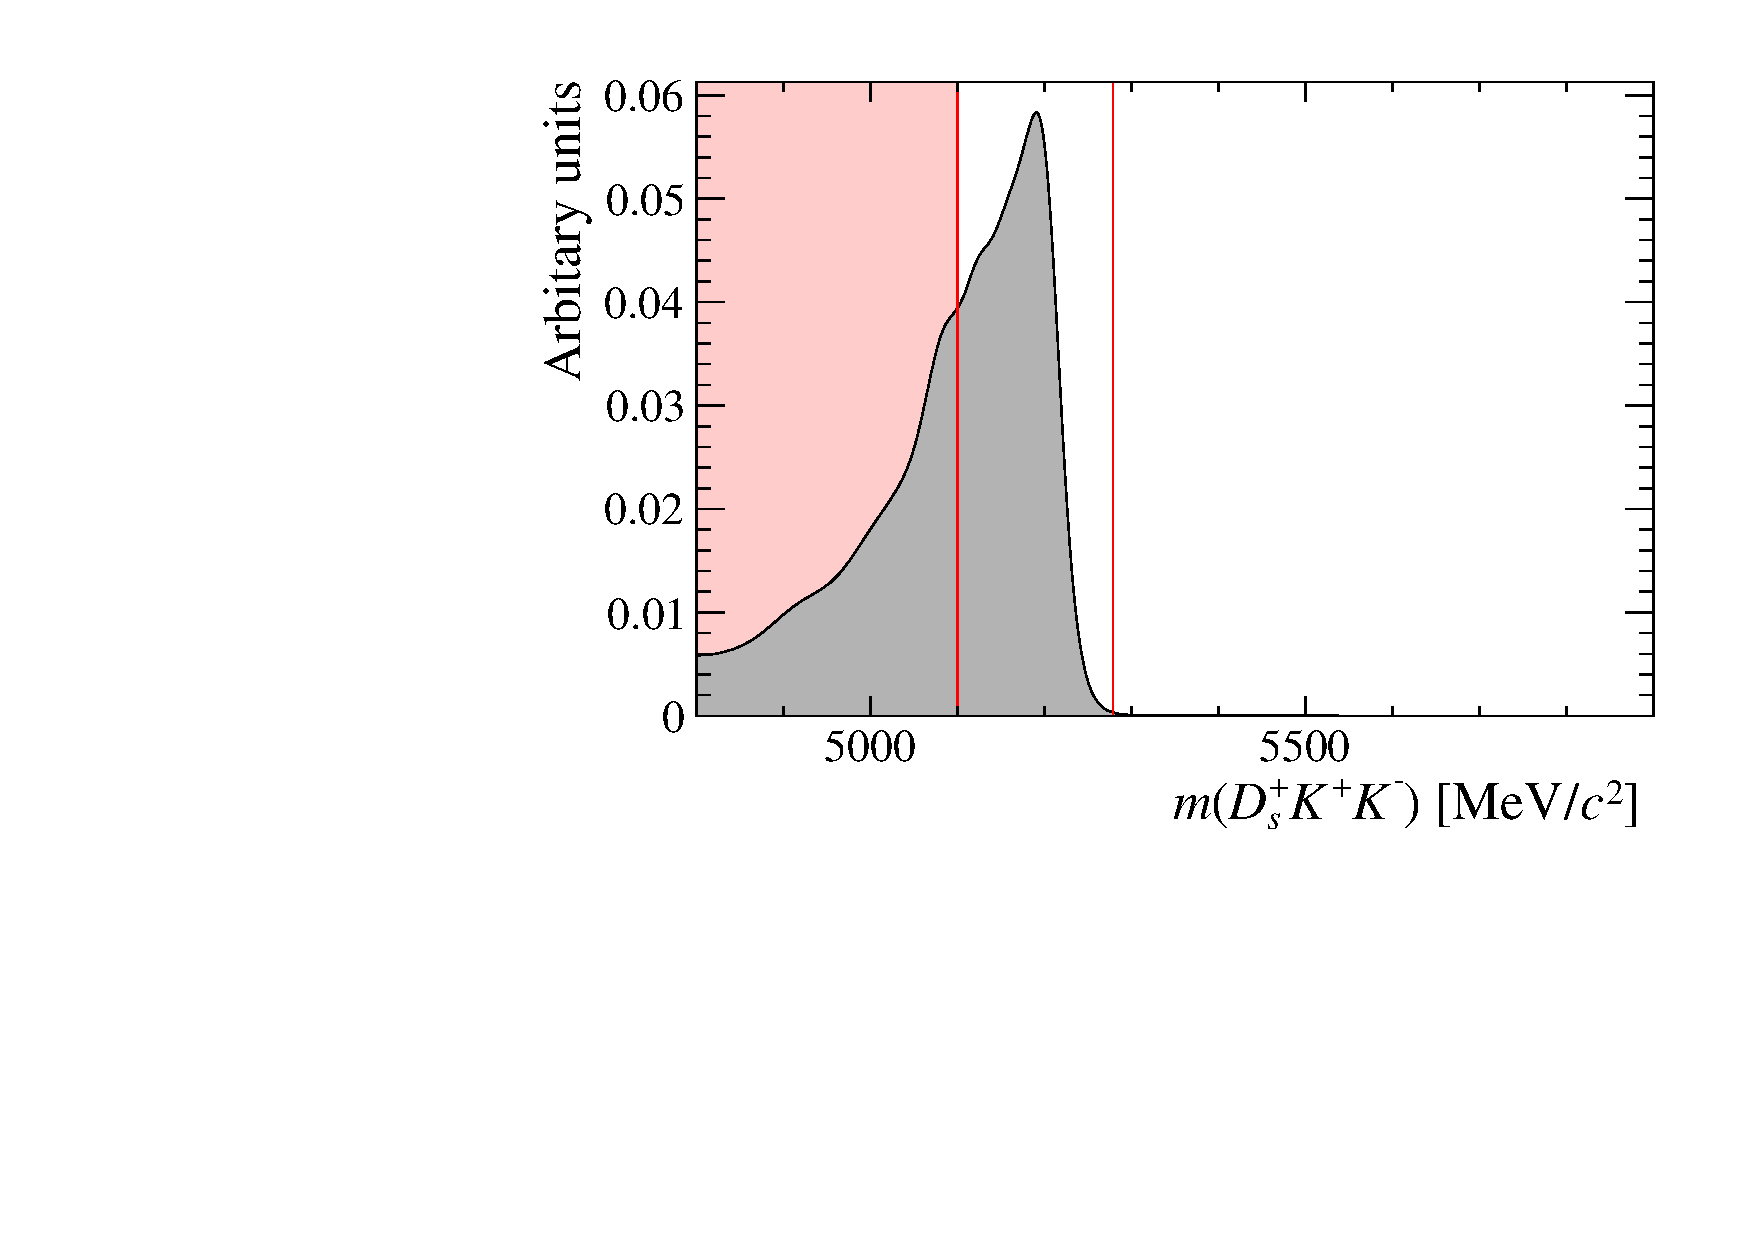
\includegraphics[width=1.0\textwidth]{figs/B2DsKK/Bs2Dsa1_4800_5900_Shape.pdf}
        \caption{\decay{\Bsb}{\Dsp\Km\Kstarz} }
        \label{fig:B2DsKK_part_reco_backgrounds_DsKKstar}
    \end{subfigure}
    \begin{subfigure}[t]{0.49\textwidth}
        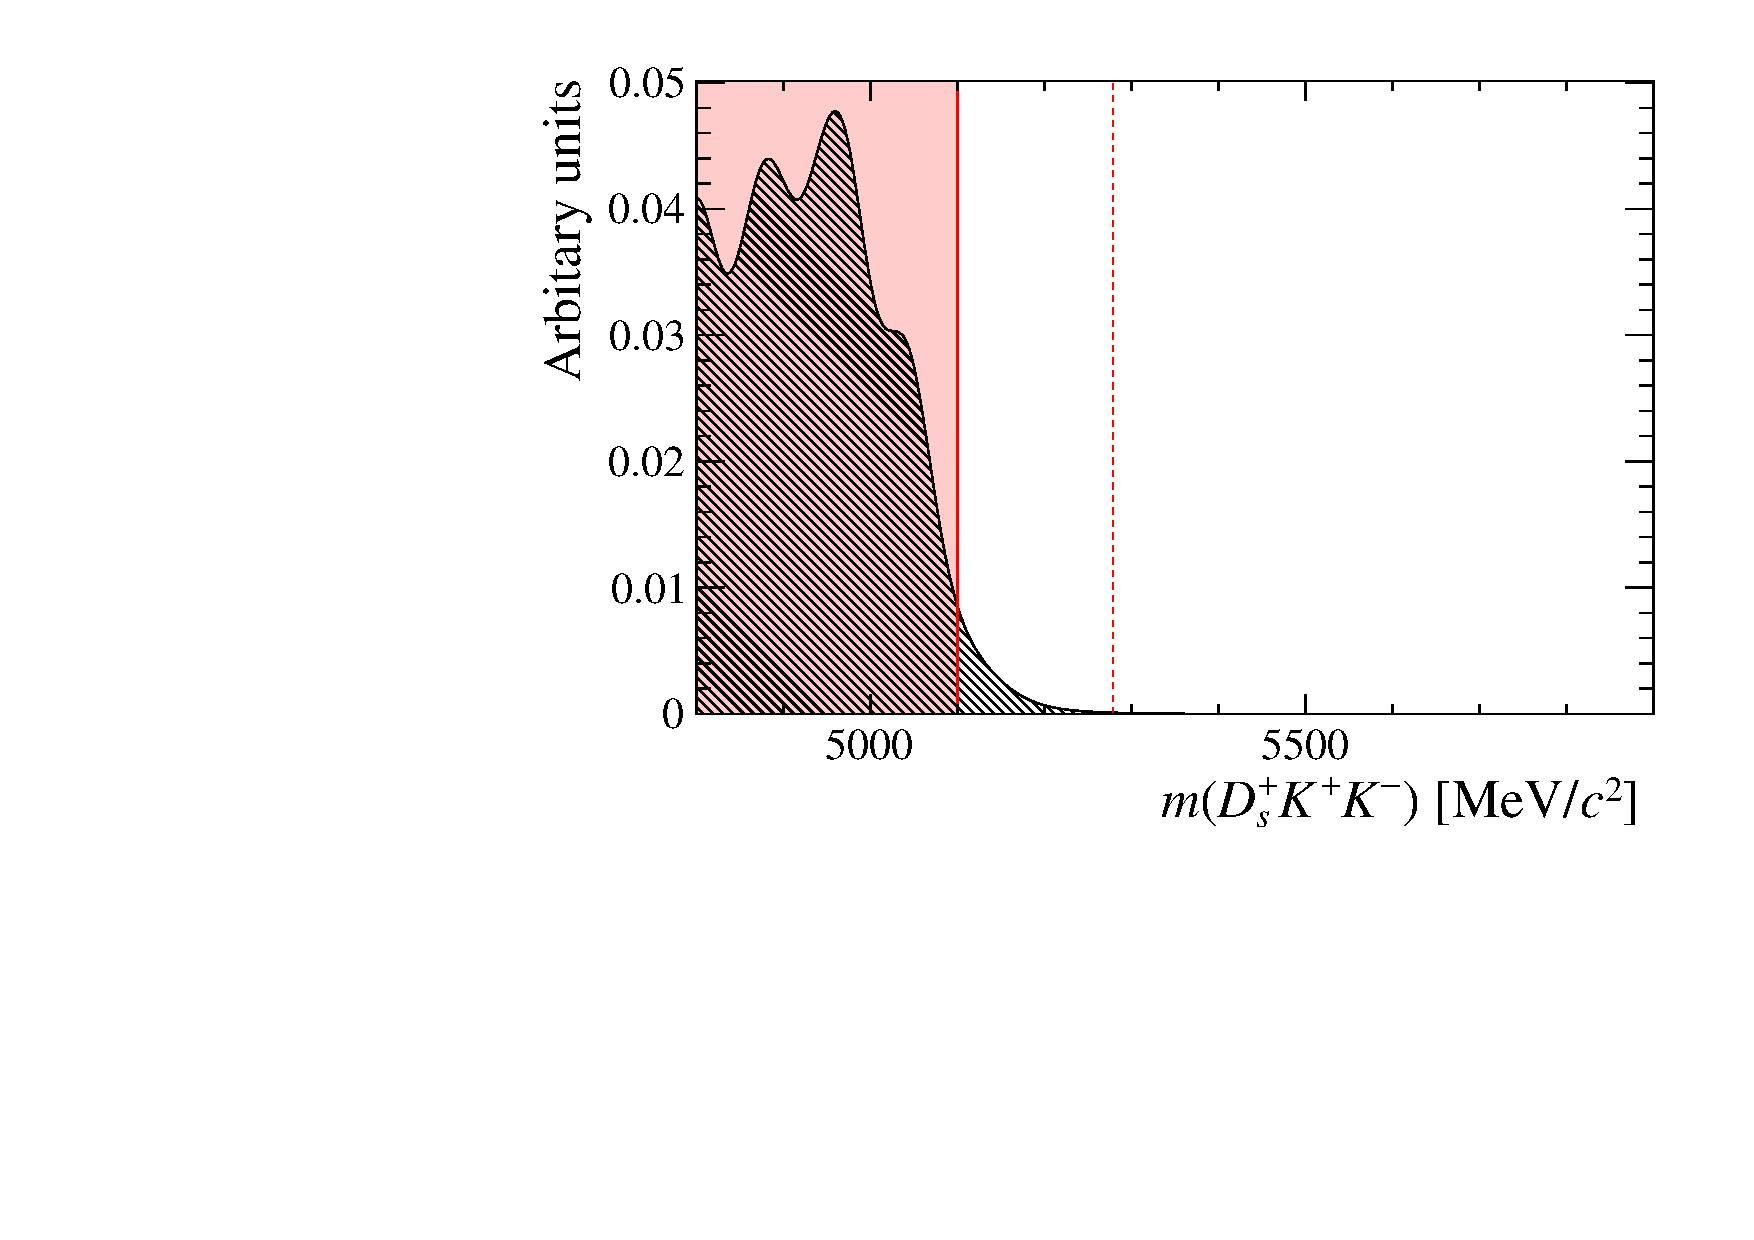
\includegraphics[width=1.0\textwidth]{figs/B2DsKK/Bs2DsstKKst_4800_5900_Shape.pdf}
        \caption{\decay{\Bsb}{\Dssp\Km\Kstarz}}
        \label{fig:B2DsKK_part_reco_backgrounds_DssKKstar}
    \end{subfigure}
    \begin{subfigure}[t]{0.49\textwidth}
        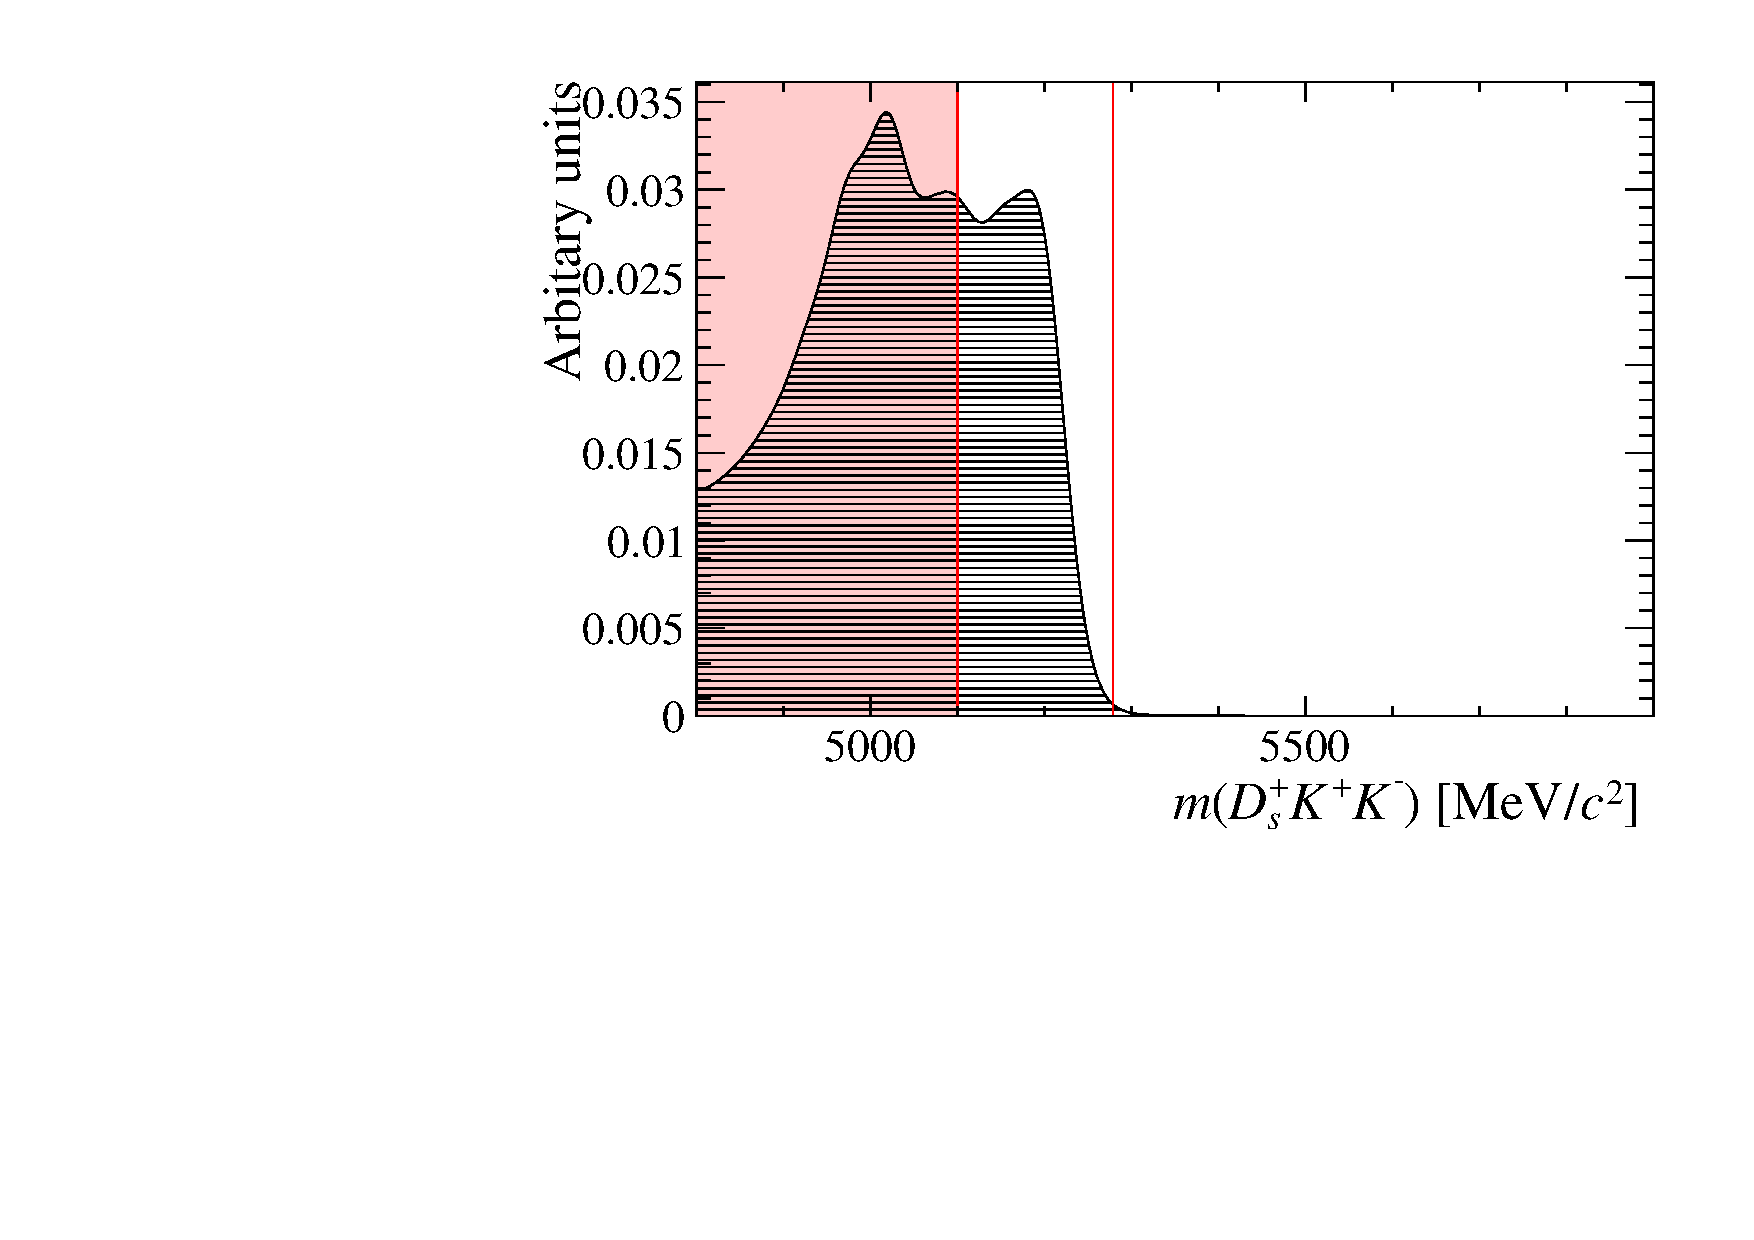
\includegraphics[width=1.0\textwidth]{figs/B2DsKK/Bs2DsDs_4800_5900_Shape.pdf}
        \caption{\decay{\Bsb}{\Dsp\Dsm} }
        \label{fig:B2DsKK_part_reco_backgrounds_DsDs}
    \end{subfigure}
    \begin{subfigure}[t]{0.49\textwidth}
        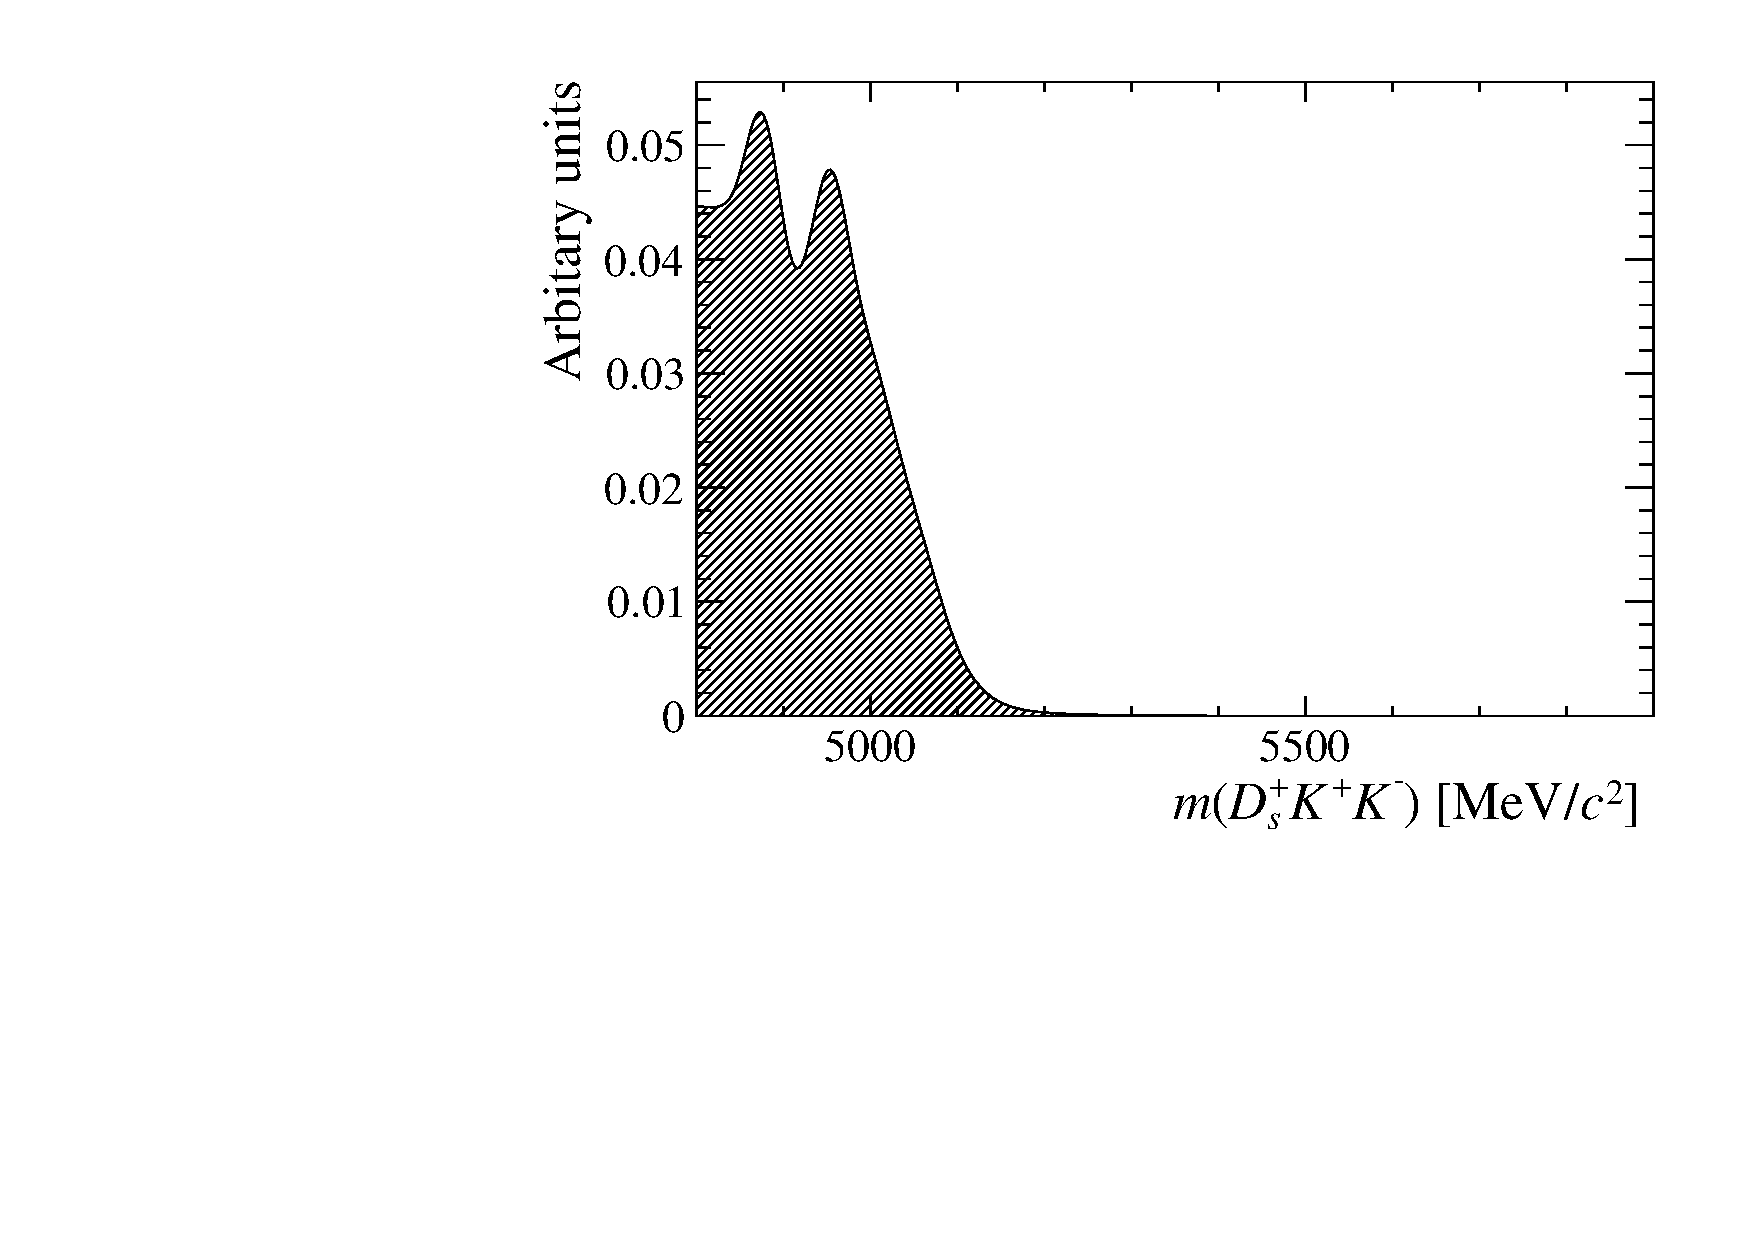
\includegraphics[width=1.0\textwidth]{figs/B2DsKK/Bs2DsstDs_4800_5900_Shape.pdf}
        \caption{\decay{\Bsb}{\Dssp\Dsm} }
        \label{fig:B2DsKK_part_reco_backgrounds_DssDs}
    \end{subfigure}
    \caption{Partially reconstructed mass PDFs. The \Bp meson mass is represented by a vertical dashed line. The range below $5100\mevcc$ (highlighted in red) is not included in the fit range.}
    \label{fig:B2DsKK_part_reco_backgrounds}   
\end{figure}
%%%%%%%%%%%%%%%%%%%%%%%%%%%%%%%%%%%%%%%%%%%%%%%%%%%%%%%%%%


% %%%%%%%%%%%%%%%%%%%%%%%%%%%%%%%%%%%%%%%%%%%%%%%%%%%%%%%%%%
% \begin{figure}[!h]
%     \centering
%     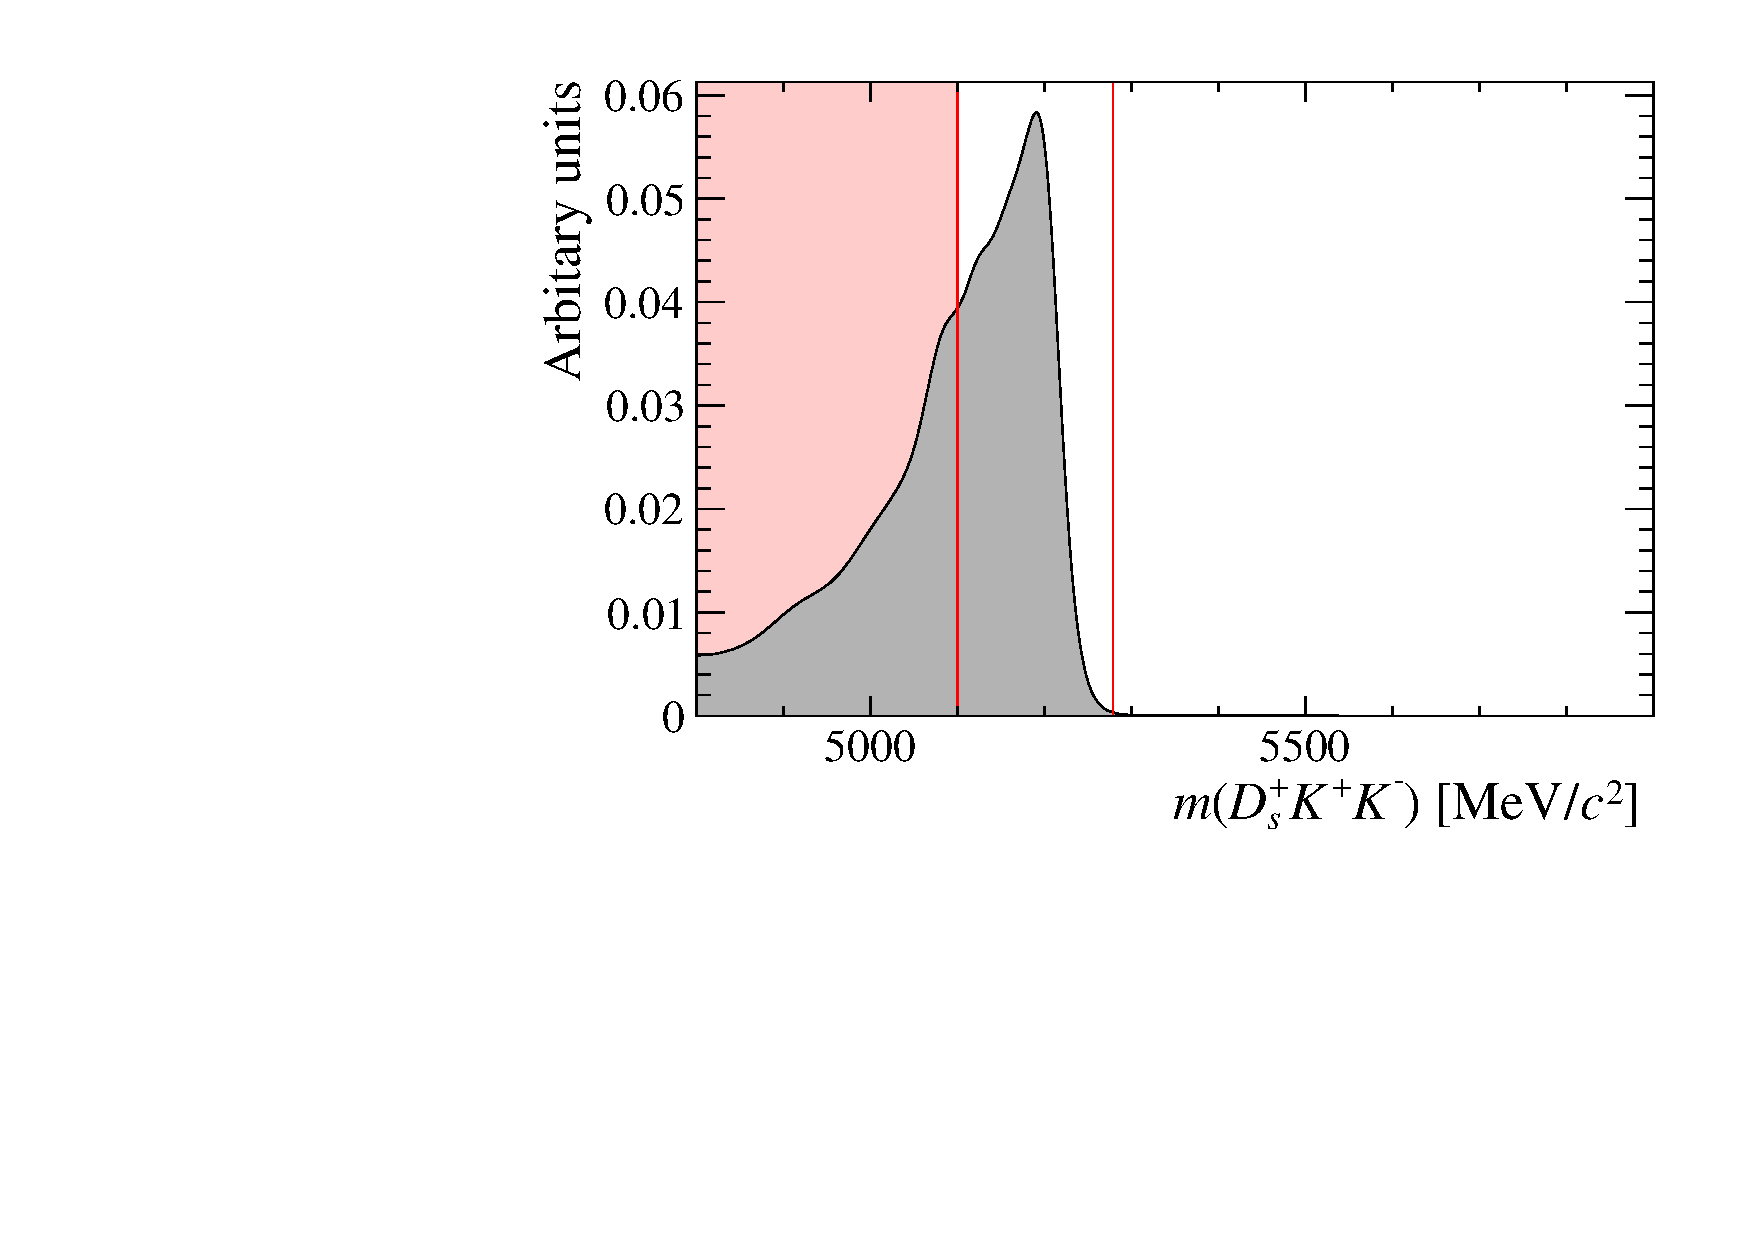
\includegraphics[width=0.49\textwidth]{figs/B2DsKK/Bs2Dsa1_4800_5900_Shape.pdf}
%     \caption{Partially reconstructed \decay{\Bsb}{\Dsp\Km\Kstarz} mass shape. The \Bp meson mass is represented by a vertical dashed line. The range below $5100\mevcc$ (highlighted in red) is not included in the fit range.}
%     \label{fig:B2DsKK_part_reco_backgrounds_DsKKstar}   
% \end{figure}
% %%%%%%%%%%%%%%%%%%%%%%%%%%%%%%%%%%%%%%%%%%%%%%%%%%%%%%%%%%

\begin{description}
\item \decay{\Bsb}{\Dssp\Km\Kstarz}: similarly this decay can form a background at low invariant mass when a soft neutral particle is not reconstructed in the \decay{\Dssp}{\Dsp X} decay in addition to the pion from the \Kstarz. This PDF is also determined using the \texttt{RooKeysPDF} class and shown in Fig.~\ref{fig:B2DsKK_part_reco_backgrounds_DssKKstar}.
\end{description}

% %%%%%%%%%%%%%%%%%%%%%%%%%%%%%%%%%%%%%%%%%%%%%%%%%%%%%%%%%%
% \begin{figure}[!h]
%     \centering
%     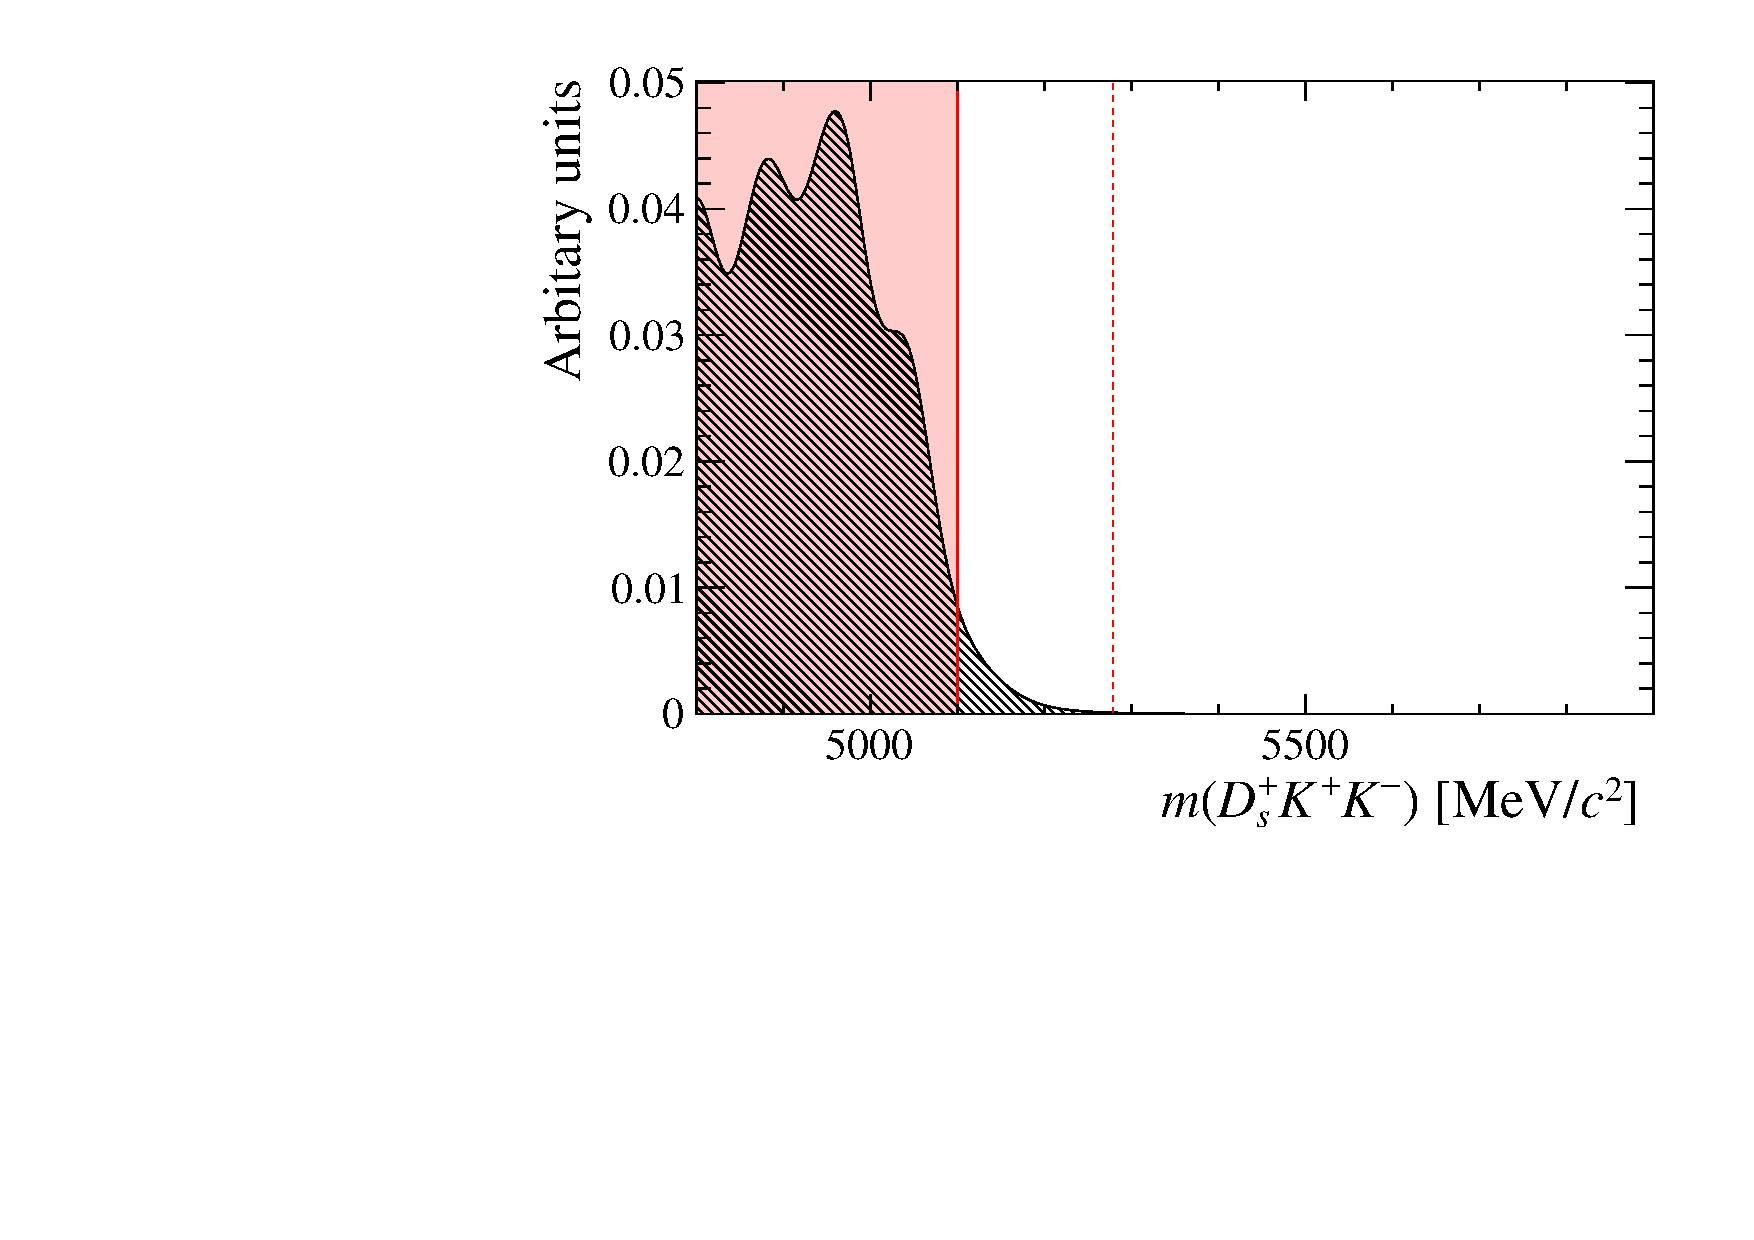
\includegraphics[width=0.49\textwidth]{figs/B2DsKK/Bs2DsstKKst_4800_5900_Shape.pdf}
%     \caption{Partially reconstructed \decay{\Bsb}{\Dssp\Km\Kstarz} mass shape. The \Bp meson mass is represented by a vertical dashed line. The range below $5100\mevcc$ (highlighted in red) is not included in the fit range.}
%     \label{fig:B2DsKK_part_reco_backgrounds_DssKKstar}   
% \end{figure}
% %%%%%%%%%%%%%%%%%%%%%%%%%%%%%%%%%%%%%%%%%%%%%%%%%%%%%%%%%%

\begin{description}
\item \decay{\Bsb}{\Dsp\Dsm}: this decay can form a background to the signal when a pion is missed from either of the \Dsp decays. This requires both \Dsp mesons to decay to the \decay{\Dsp}{\Kp\Km\pip} final state. 
%Due to the large phase-space of \decay{\Dsp}{\Kp\Km\pip} decays, the pion is not as soft as in the previous background modes. 
%Therefore this background only becomes significant at smaller invariant masses as shown in Fig.~\ref{fig:B2DsKK_part_reco_backgrounds}. 
This background becomes significant at close to the \Bp meson mass as shown in Fig.~\ref{fig:B2DsKK_part_reco_backgrounds_DsDs}. 
This PDF is similarly determined by creating a kernel estimation of fully-reconstructed simulated events passing the signal selection.  
\end{description}

% %%%%%%%%%%%%%%%%%%%%%%%%%%%%%%%%%%%%%%%%%%%%%%%%%%%%%%%%%%
% \begin{figure}[!h]
%     \centering
%     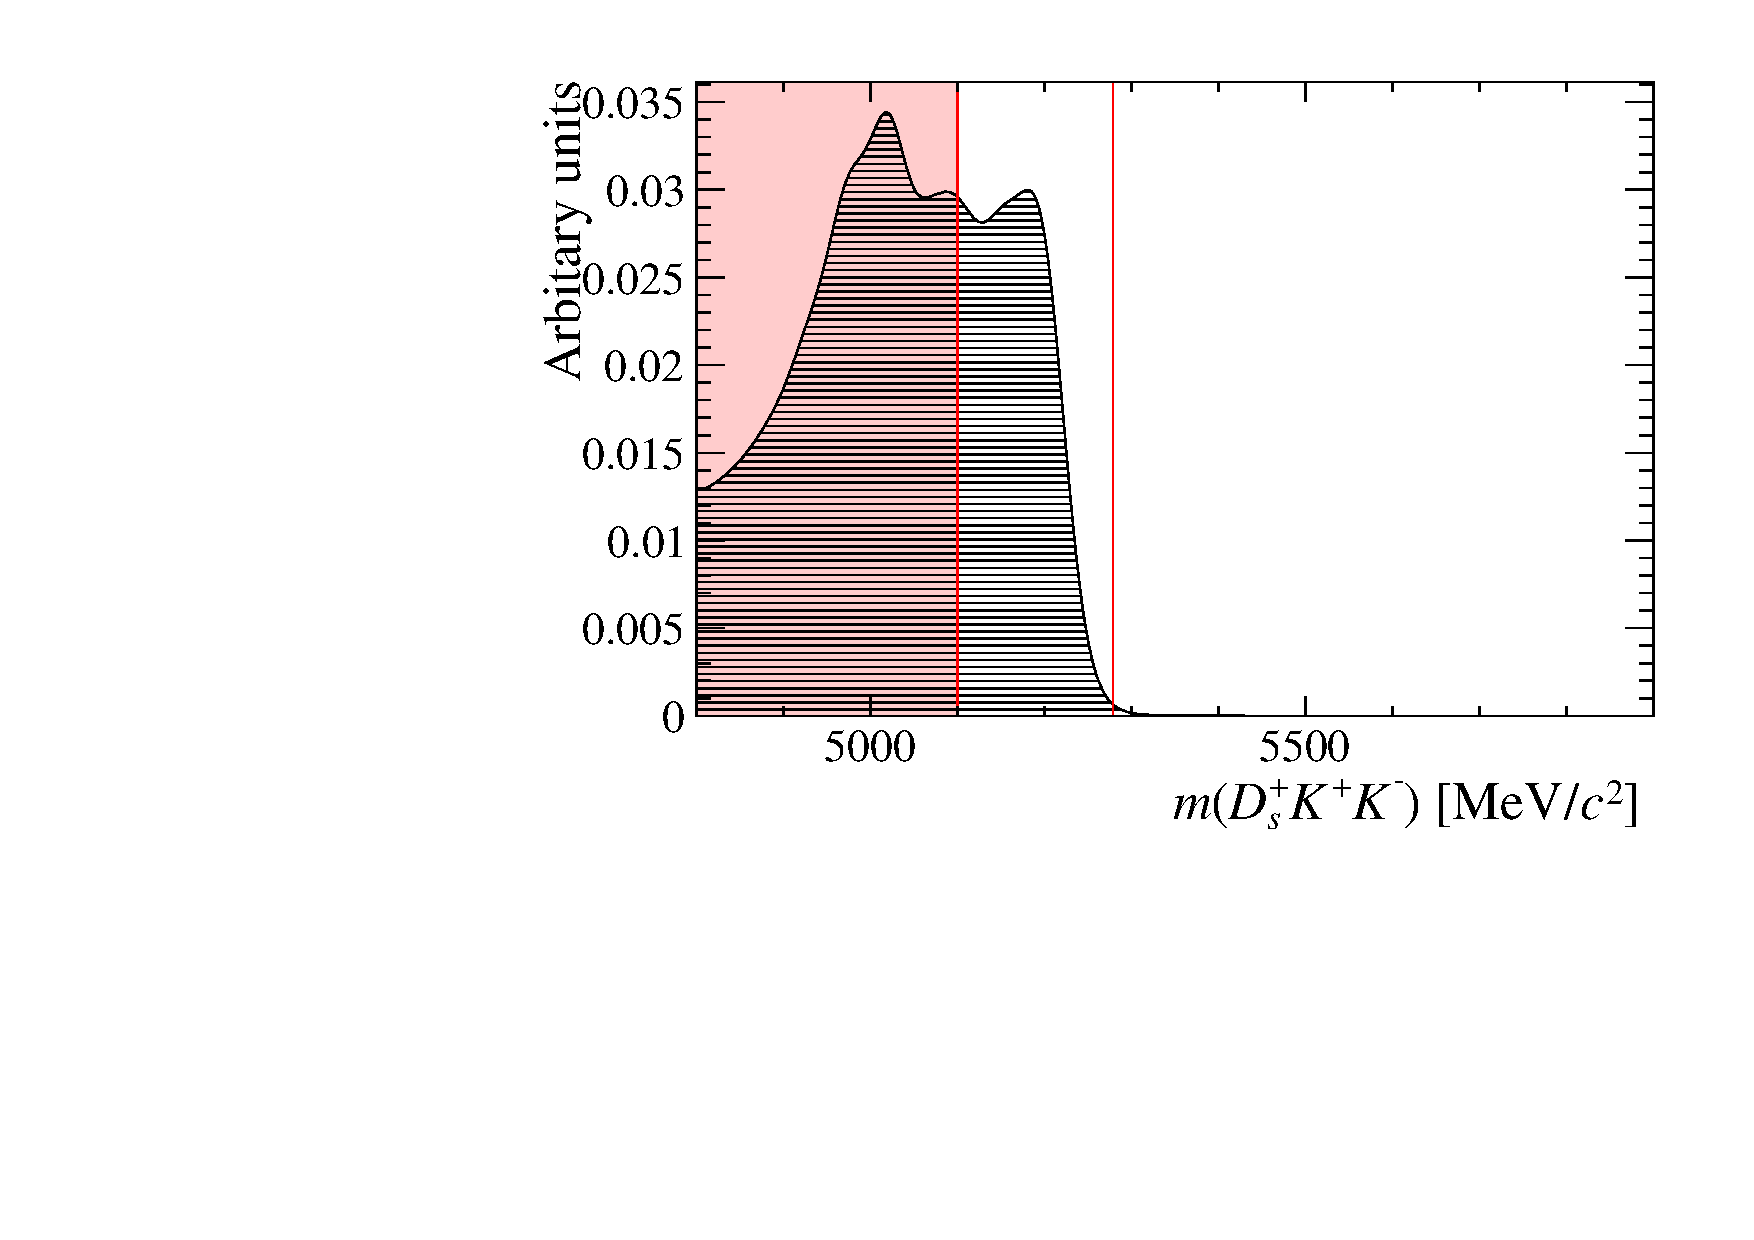
\includegraphics[width=0.49\textwidth]{figs/B2DsKK/Bs2DsDs_4800_5900_Shape.pdf}
%     \caption{Partially reconstructed \decay{\Bsb}{\Dsp\Dsm} mass shape. The \Bp meson mass is represented by a vertical dashed line. The range below $5100\mevcc$ (highlighted in red) is not included in the fit range.}
%     \label{fig:B2DsKK_part_reco_backgrounds_DsDs}   
% \end{figure}
% %%%%%%%%%%%%%%%%%%%%%%%%%%%%%%%%%%%%%%%%%%%%%%%%%%%%%%%%%%

\begin{description}
\item \decay{\Bzb}{\Dsp\Dm}: this decay can form a background when both the \Dsp and \Dm mesons decay to the \Kpm\Kmp\pipm final state. Due to the similar topology to the \decay{\Bsb}{\Dsp\Dsm} decay, the same PDF determined from simulated events is used, however it is shifted down in mass by 40\mevcc to account for the difference in kinematics. The mode \decay{\Dp}{\Kp\Km\pip} is Cabibbo suppressed with respect to \decay{\Dsp}{\Kp\Km\pip}.

\item \decay{\Bsb}{\Dssp\Dsm}: similarly this decay can cause a background when both a soft neutral particle is missed from the \decay{\Dssp}{\Dsp X} decay as well as a pion from either of the \Dsp mesons. As such this only has a small contribution within the fit range as shown in Fig.~\ref{fig:B2DsKK_part_reco_backgrounds_DssDs}. 
\end{description}

% %%%%%%%%%%%%%%%%%%%%%%%%%%%%%%%%%%%%%%%%%%%%%%%%%%%%%%%%%%
% \begin{figure}[!h]
%     \centering
%     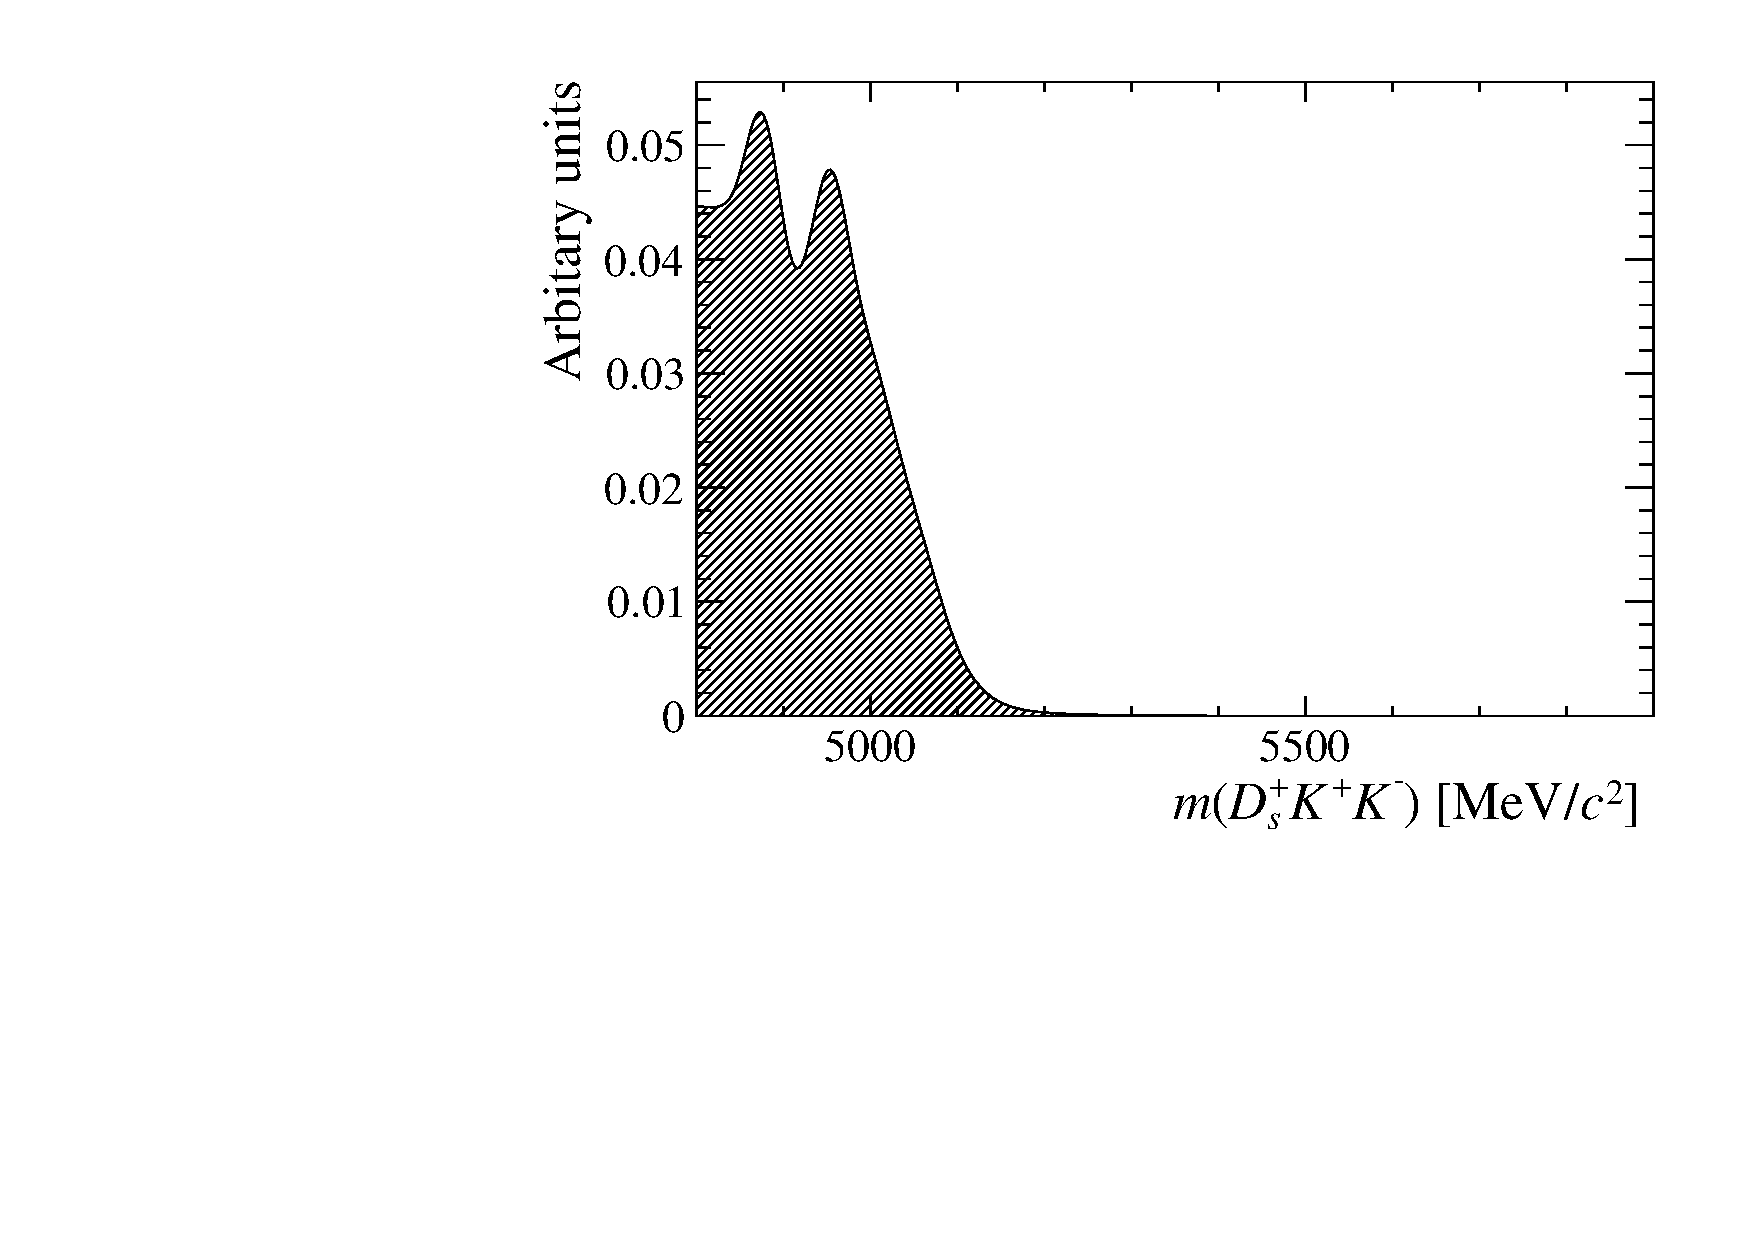
\includegraphics[width=0.49\textwidth]{figs/B2DsKK/Bs2DsstDs_4800_5900_Shape.pdf}
%     \caption{Partially reconstructed \decay{\Bsb}{\Dssp\Dsm} mass shape.}
%     \label{fig:B2DsKK_part_reco_backgrounds_DssDs}   
% \end{figure}
% %%%%%%%%%%%%%%%%%%%%%%%%%%%%%%%%%%%%%%%%%%%%%%%%%%%%%%%%%%


All PDFs determined using kernel estimations from simulated events are convolved with a Gaussian distribution to account for difference between the simulations and data. The mean position of the Gaussian is given by a single free parameter $\delta$, allowing these PDF to move slightly high or lower in mass. The width of the Gaussian is increased by 4\mevcc to account for the difference in resolution between simulation and data determined from the normalisation channel.



\subsection{Combinatorial  background}
\label{sec:B2DsKK_combcomps}

The dominant source of background under the signal peak is due to combinations of unrelated tracks. This combinatorial background is modelled using an exponential function 
\begin{equation}
f(m|c) = e^{-mc},
\end{equation}
where $c$ is the effective slope of the function and $m$ is the observable \Bp meson invariant mass. The separate fits to the signal and normalisation modes have the freedom to have different combinatorial slopes.




\section{Free and constrained parameters}


The signal  and normalisation mass fits have eleven and nine free parameters respectively. These can vary to find a best fit to the data. These parameters are of three types: parameter of interest, PDF shape parameters and yields.
The parameters of interest in the two fits are $N(\decay{\Bp}{\Dsp\Kp\Km})$ and $N(\decay{\Bp}{\Dsp\Dzb})$.
The signal and normalisation fits have four and five free parameters that determine the PDF shapes. 
The yields of each background component are left free in the signal fit. This corresponds to six free parameters for $N_{\text{comb}}$, $N(\decay{\Bsb}{\Dsp\Km\Kstarz})$, $N(\decay{\Bsb}{\Dssp\Km\Kstarz})$, $N(\decay{\Bs}{\Dsp\Dsm})$, $N(\decay{\Bz}{\Dsp\Dm})$, and $N(\decay{\Bs}{\Dssp\Dsm})$. The yields of the combinatorial and partially reconstructed backgrounds are left free in the fit to the normalisation channel. This corresponds to three parameters; $N_{\text{comb}}$, $N(\decay{\Bp}{\Dssp\Dzb})$ and $N(\decay{\Bp}{\Dsp\Dstarzb})$. The relatives contributions of the \decay{\Dssp}{\Dsp\piz} and \decay{\Dssp}{\Dsp\Pgamma} decays are fixed to their ratio of branching fractions (similarly for \Dstarzb). A factor is included to account for the fraction of each PDF that is within the fitted \Bp invariant mass range.


% \subsection{Parameter of interest}
% \begin{description}
% \item \textbf{Signal fit:} the parameter of interest in the signal decay is $N(\decay{\Bp}{\Dsp\Kp\Km})$, the yield attributed to the signal PDF.

% \item \textbf{Normalisation fit:} the parameter of interest in the signal decay is $N(\decay{\Bp}{\Dsp\Dzb})$, the yield attributed to the normalisation PDF. 

% \end{description}

%           %         nsig    4.4287e+02    4.4277e+02 +/-  2.94e+01  <none>
%           %         nsig    1.0905e+03    1.0905e+03 +/-  3.42e+01  <none>

% \subsection{Shape parameters}
% \begin{description}
% \item \textbf{Signal fit:} The signal fit contains four free parameters that determine the shape of various PDFs. This corresponds to the mass offset $\delta$ for the partially reconstructed backgrounds, signal mean value $\mu$, signal width $\sigma_{1}$ and combinatorial slope $c$.
%           % global_shift    2.2538e+00    3.5457e+00 +/-  1.17e+01  <none>
%           %       mean_B    5.2789e+03    5.2789e+03 +/-  8.82e-01  <none>
%           %        sigma    1.2298e+01    1.2291e+01 +/-  8.77e-01  <none>
%           %        slope   -2.8199e-03   -2.8202e-03 +/-  2.79e-04  <none>
% \item \textbf{Normalisation fit:} The normalisation fit has five free parameters that control the distributions of the signal and background PDFs. This includes the mean \Bp mass $\mu$, signal width $\sigma_{1}$, the combinational slope $c$, the mass offset $\delta$ for the partially reconstructed backgrounds and the relative heights of the double peaked partially reconstructed shapes $\xi$.   
%           %   global_csi    1.2683e-06    5.2233e-08 +/-  2.25e-01  <none>
%           % global_shift   -1.0585e+01   -1.0586e+01 +/-  1.31e+00  <none>
%           %       mean_B    5.2784e+03    5.2784e+03 +/-  4.00e-01  <none>
%           %        slope   -9.4305e-03   -9.4308e-03 +/-  1.13e-03  <none>
%           %        sigma    1.2436e+01    1.2435e+01 +/-  3.23e-01  <none>
% \end{description}

% \subsection{Yields}
% \begin{description}
% \item \textbf{Signal fit:} the yields of each background component are left free in the signal fit. This corresponds to six free parameters for $N_{\text{comb}}$, $N(\decay{\Bsb}{\Dsp\Km\Kstarz})$, $N(\decay{\Bsb}{\Dssp\Km\Kstarz})$, $N(\decay{\Bs}{\Dsp\Dsm})$, $N(\decay{\Bz}{\Dsp\Dm})$, and $N(\decay{\Bs}{\Dssp\Dsm})$.

%           %          nBG    1.1139e+03    1.1142e+03 +/-  7.30e+01  <none>
%           %     nBs2Dsa1    1.1153e+03    1.1147e+03 +/-  4.61e+02  <none>
%           % nBs2DsstKKst    2.9756e+02    2.9691e+02 +/-  1.24e+02  <none>
%           %     nBs2DsDs    2.0262e+02    2.0307e+02 +/-  5.08e+02  <none>
%           %      nB02DsD    4.6587e+02    4.6621e+02 +/-  1.54e+02  <none>
%           %   nBs2DsstDs    1.1208e-04    6.2385e-02 +/-  3.98e+02  <none>
% \item \textbf{Normalisation fit:} the yields of the combinatorial and partially reconstructed backgrounds are left free in the fit to the normalisation channel. This corresponds to three parameters; $N_{\text{comb}}$, $N(\decay{\Bp}{\Dssp\Dzb})$ and $N(\decay{\Bp}{\Dsp\Dstarzb})$. The relatives contributions of the \decay{\Dssp}{\Dsp\piz} and \decay{\Dssp}{\Dsp\Pgamma} decays are fixed to their ratio of branching fractions (similarly for \Dstarzb). A factor is included to account for the fraction of each PDF that is within the fitted \Bp invariant mass range.
% \end{description}

%           %          nBG    2.4773e+02    2.4769e+02 +/-  5.42e+01  <none>
%           %      nDsDst0    3.3055e+02    3.3055e+02 +/-  6.72e+01  <none>
%           %      nDsstD0    7.5230e+02    7.5220e+02 +/-  5.48e+01  <none>



\section{Fit validation}
\label{sec:B2DsKK_fitvalidation}

The fitting framework is validated by generating pseudo-experiment datasets and fitting them with the PDF model. The error in the normalisation yield is found to be overestimated by the fit model. When propagated to the final branching fraction, this effect is reduced, therefore no attempt is made to correct it. The validation studies are detailed in Appendix~\ref{sec:app_toys_B2DsKK}.

%The free parameters are treated using the plug-in method~\cite{plugin}; the generated values of all free parameters are \emph{plugged in} from the best fit to data.      

% The fitted values and uncertainties are determined for each pseudo-experiment and a corresponding pull determined, defined as
% \begin{equation}
% g_{\text{pull}} = \frac{x_{\text{fit}} - x_{\text{gen}} }{\sigma}
% \end{equation}
% where $x_{\text{gen}}$ and $x_{\text{fit}}$ are the generated and fitted values of the variable, and $\sigma$ is the parameter's uncertainty.
% For an ideal unbiased fit model, the pull of each parameter of interest would be normally distributed with unit width and mean of zero.  


% %%%%%%%%%%%%%%%%%%%%%%%%%%%%%%%%%%%%%%%%%%%%%%%%%%%%%%%%%%
% \begin{figure}[!h]
%    \centering
%    \begin{subfigure}[t]{1.0\textwidth}
%       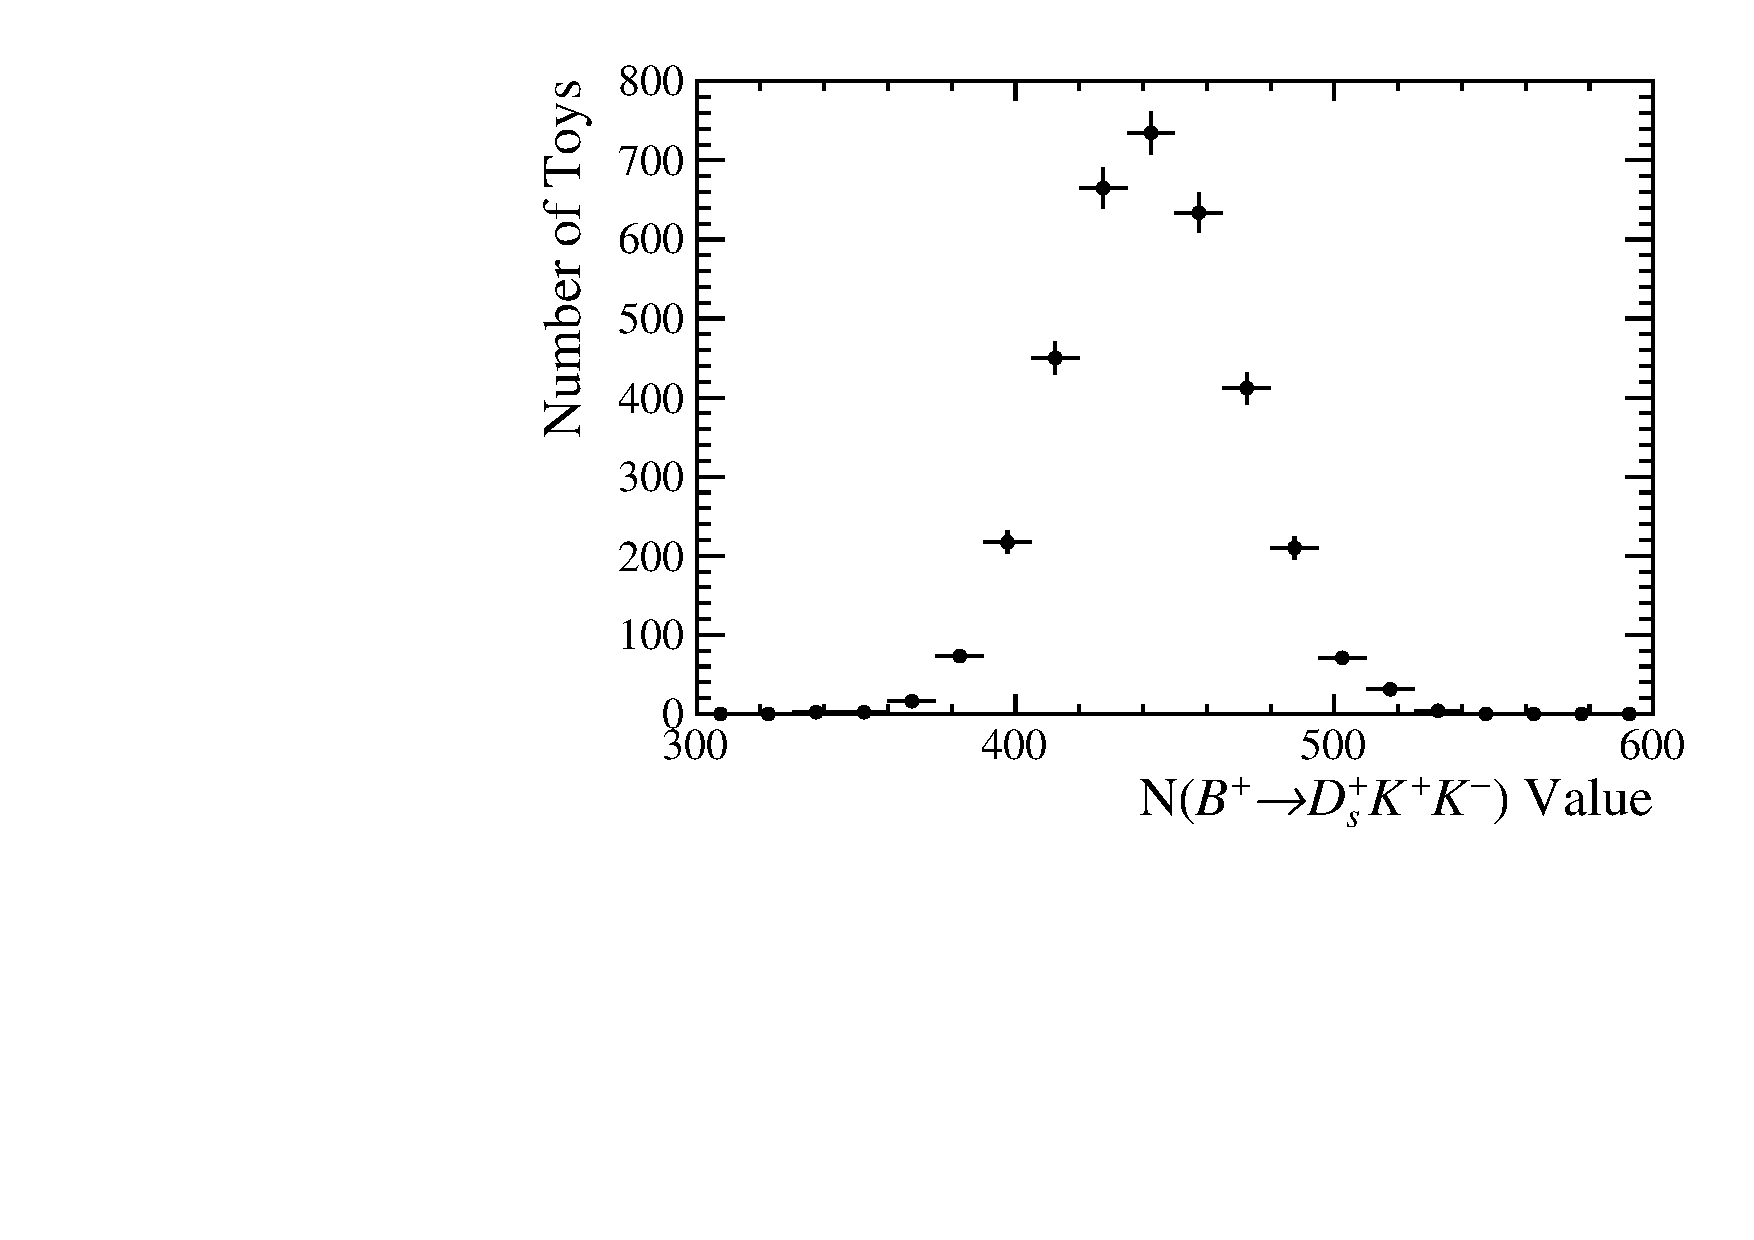
\includegraphics[width=0.32\textwidth]{figs/B2DsKK/Plots_DsKK_nsig_val.pdf}
%       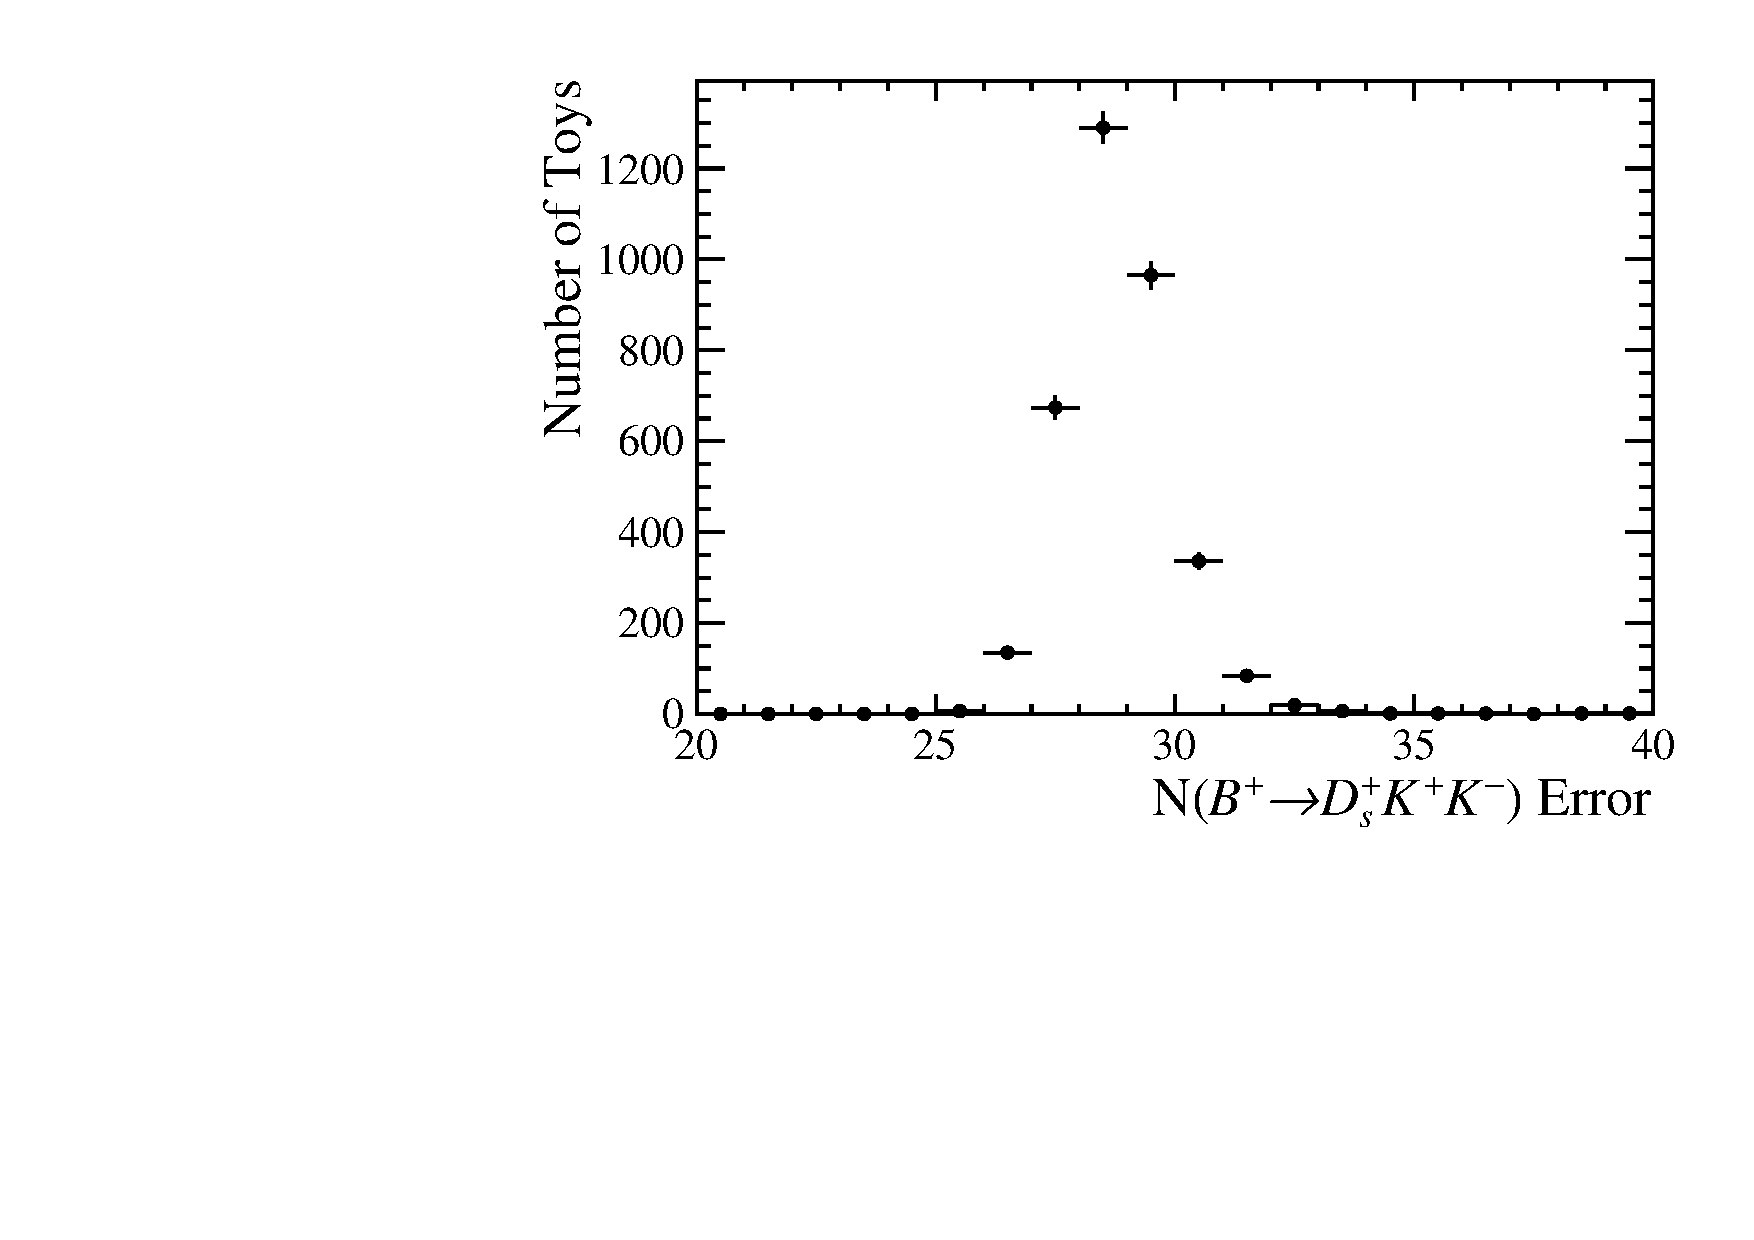
\includegraphics[width=0.32\textwidth]{figs/B2DsKK/Plots_DsKK_nsig_err.pdf}
%       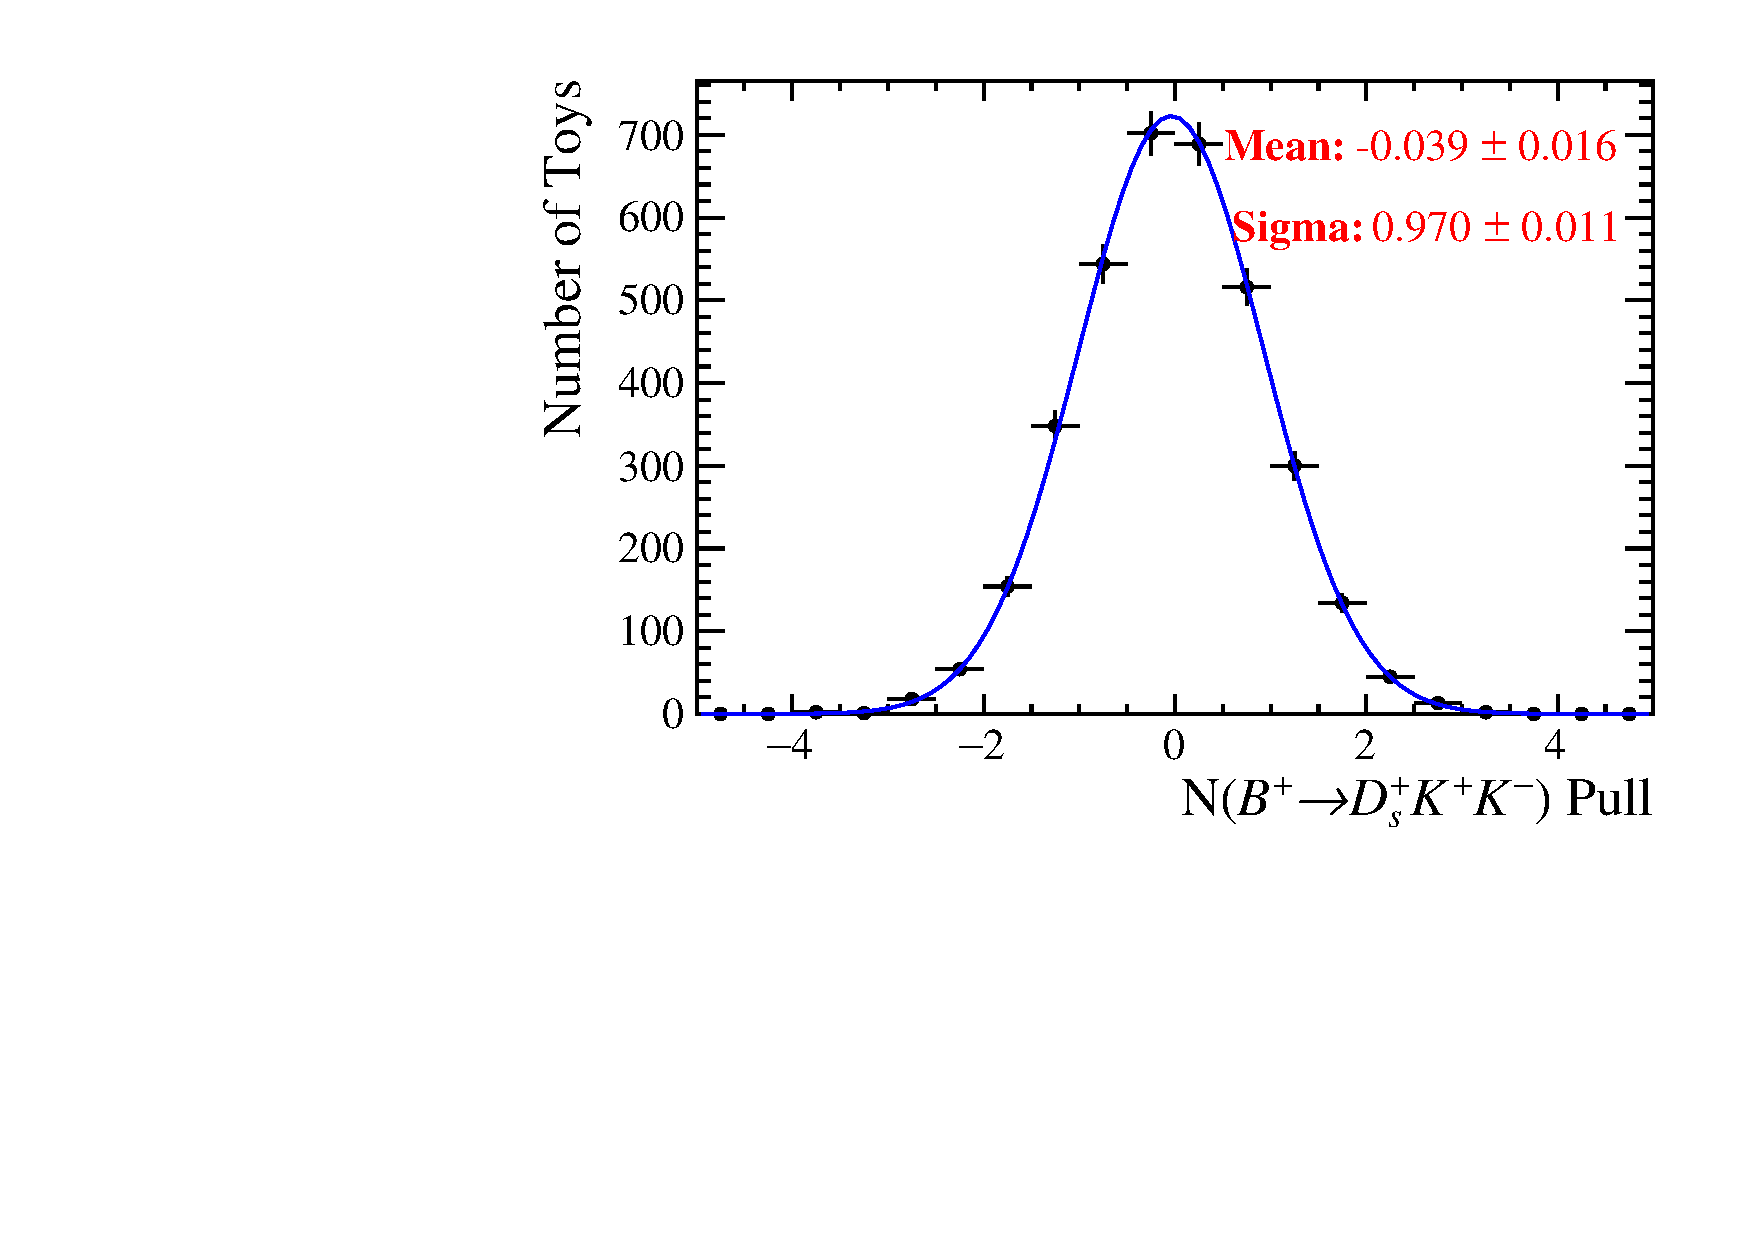
\includegraphics[width=0.32\textwidth]{figs/B2DsKK/Plots_DsKK_nsig_pul.pdf}
%       \caption{Signal fit}
%    \end{subfigure}\\
%    \begin{subfigure}[t]{1.0\textwidth}
%       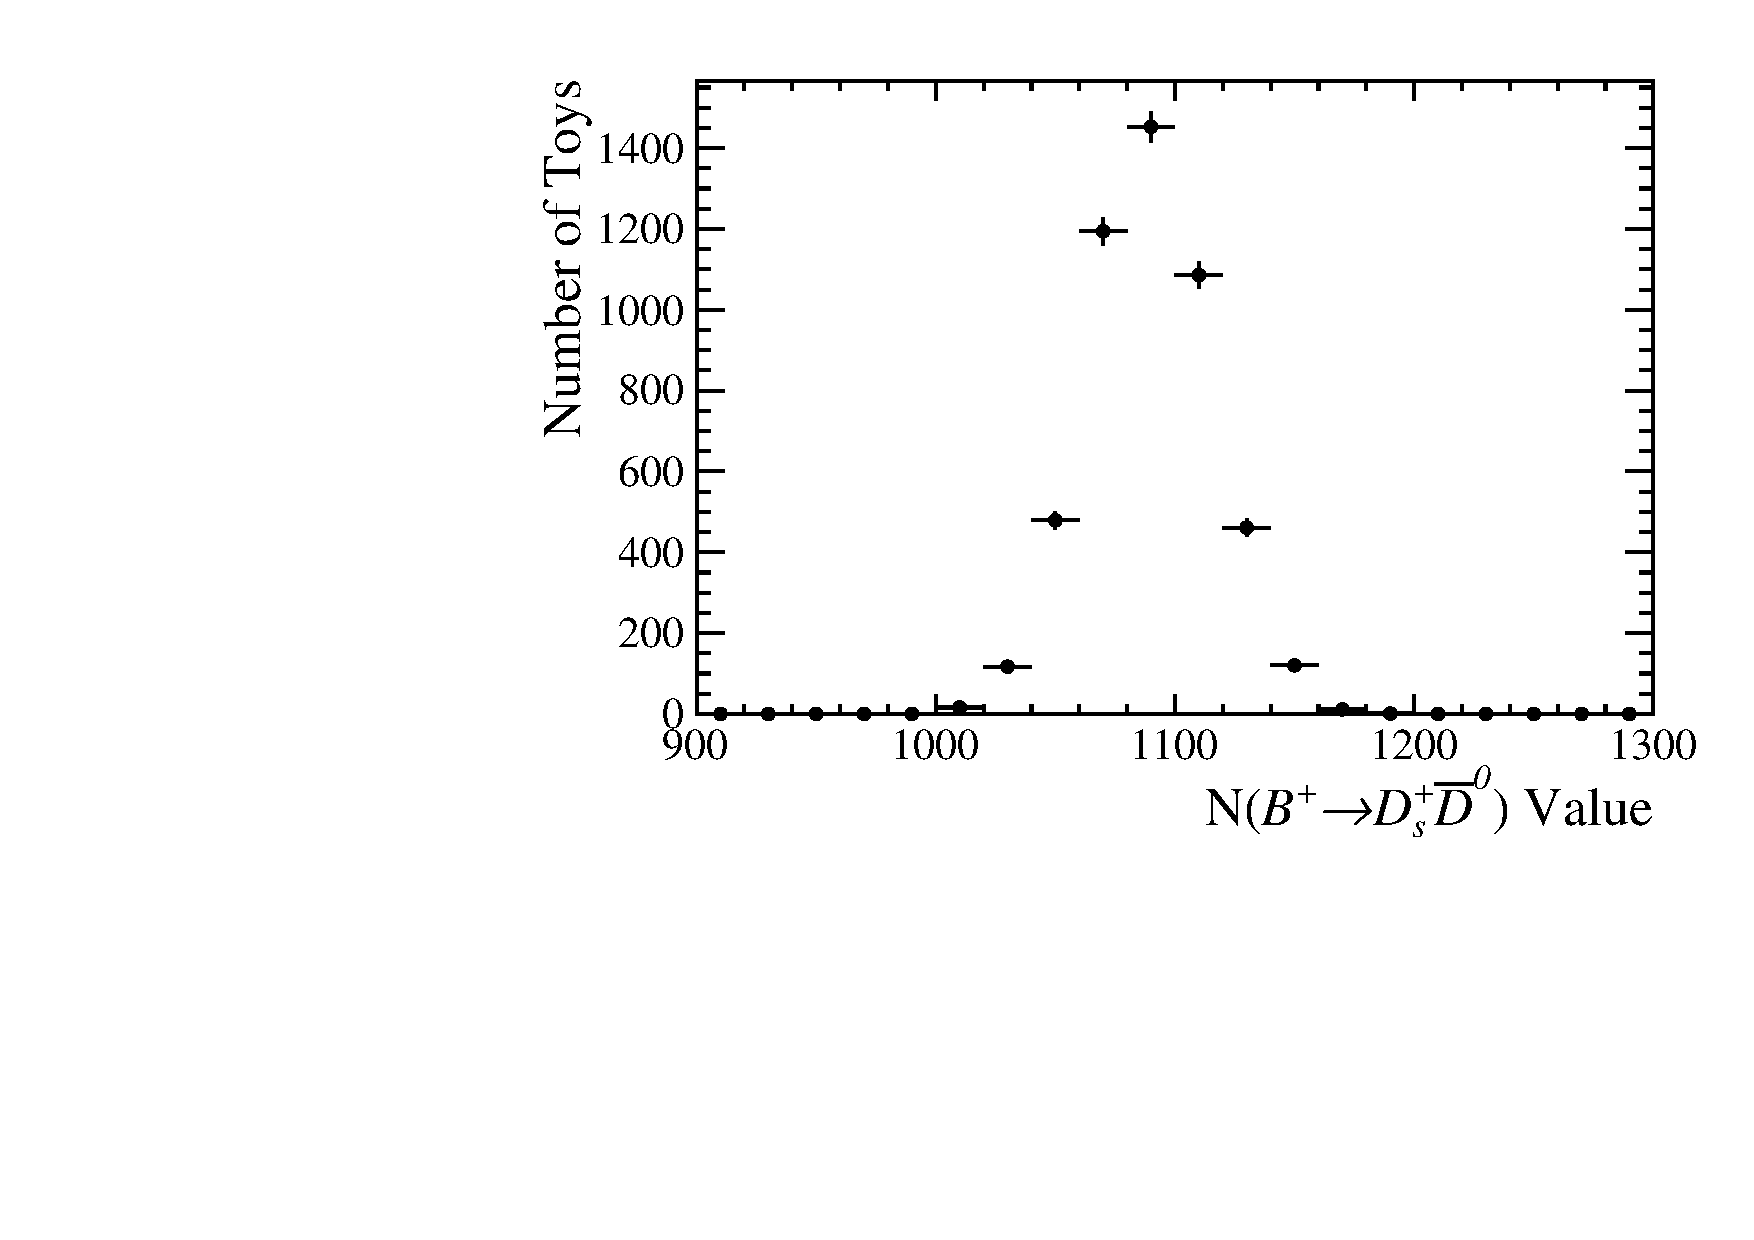
\includegraphics[width=0.32\textwidth]{figs/B2DsKK/Plots_DsD0_nsig_val.pdf}
%       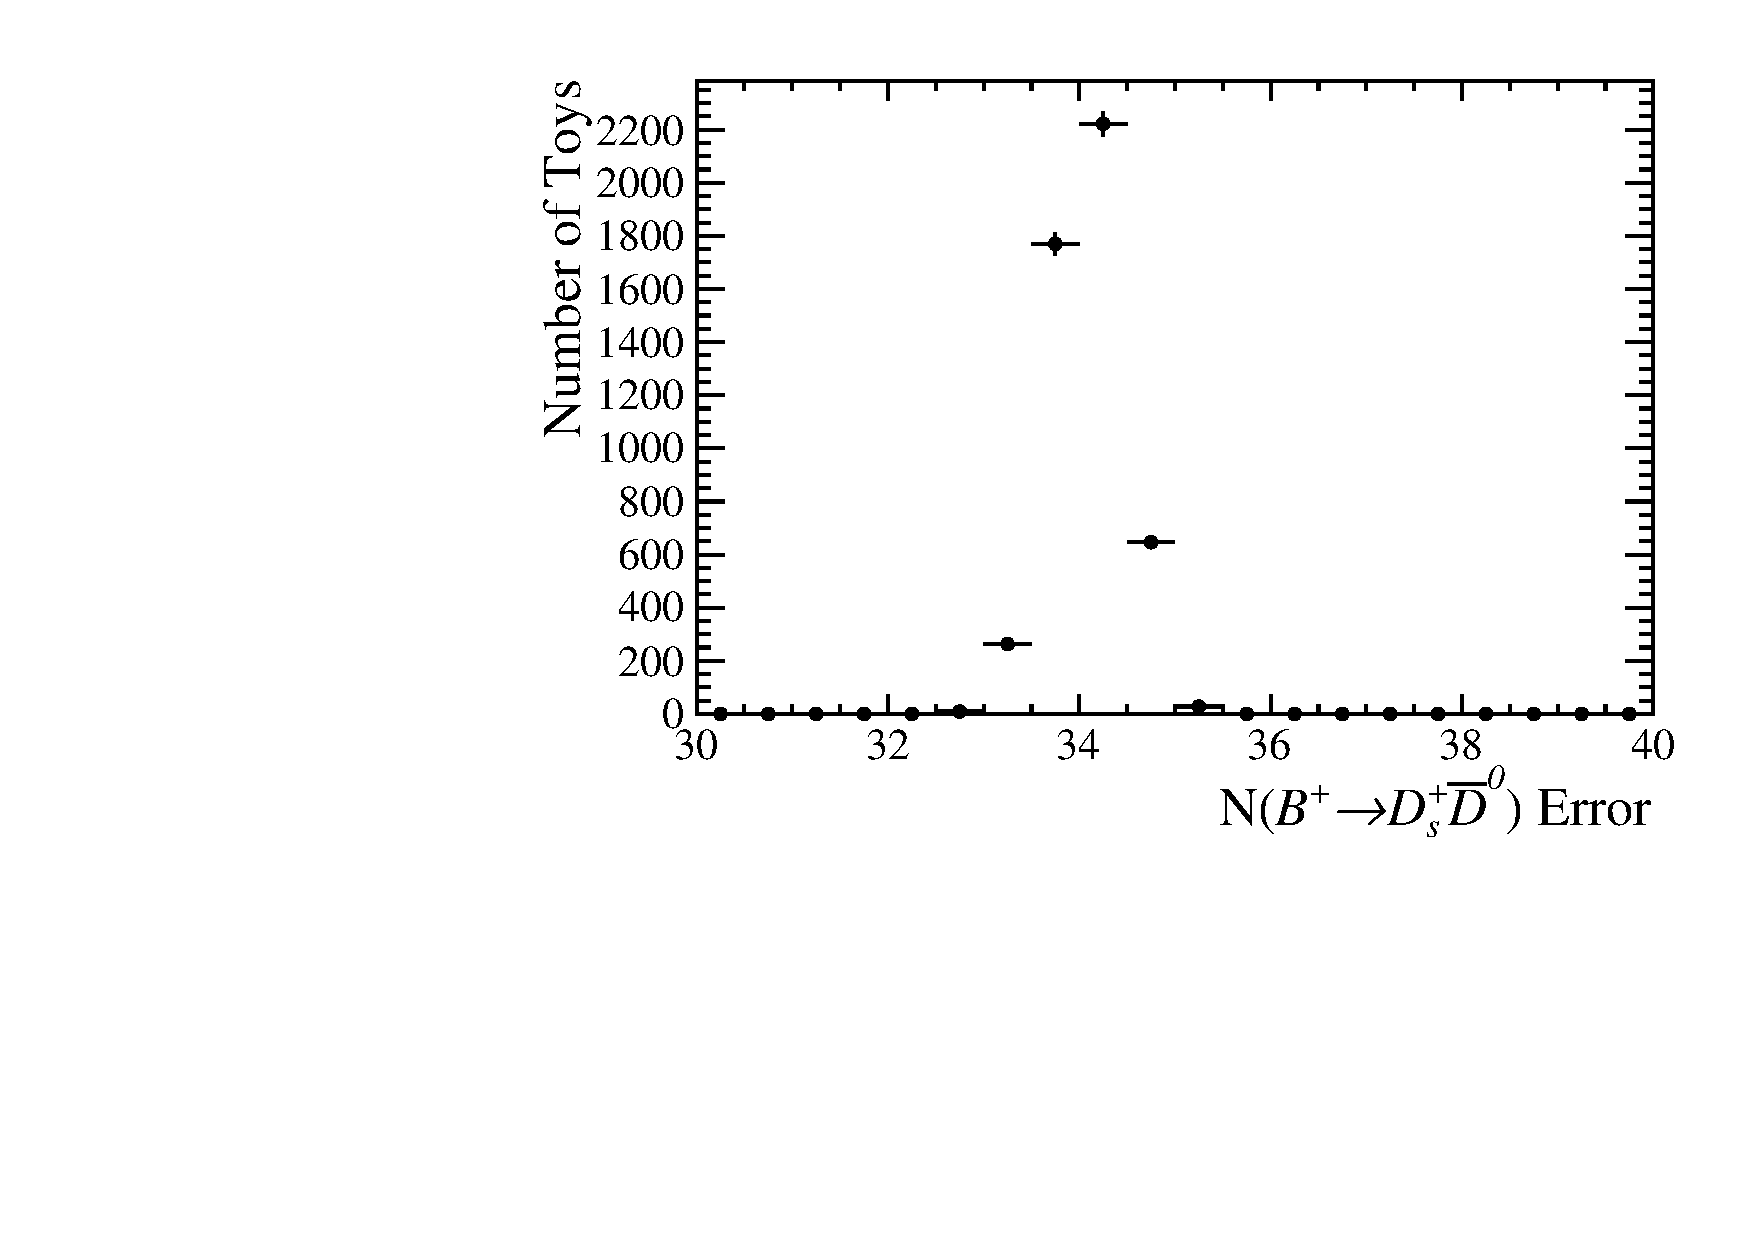
\includegraphics[width=0.32\textwidth]{figs/B2DsKK/Plots_DsD0_nsig_err.pdf}
%       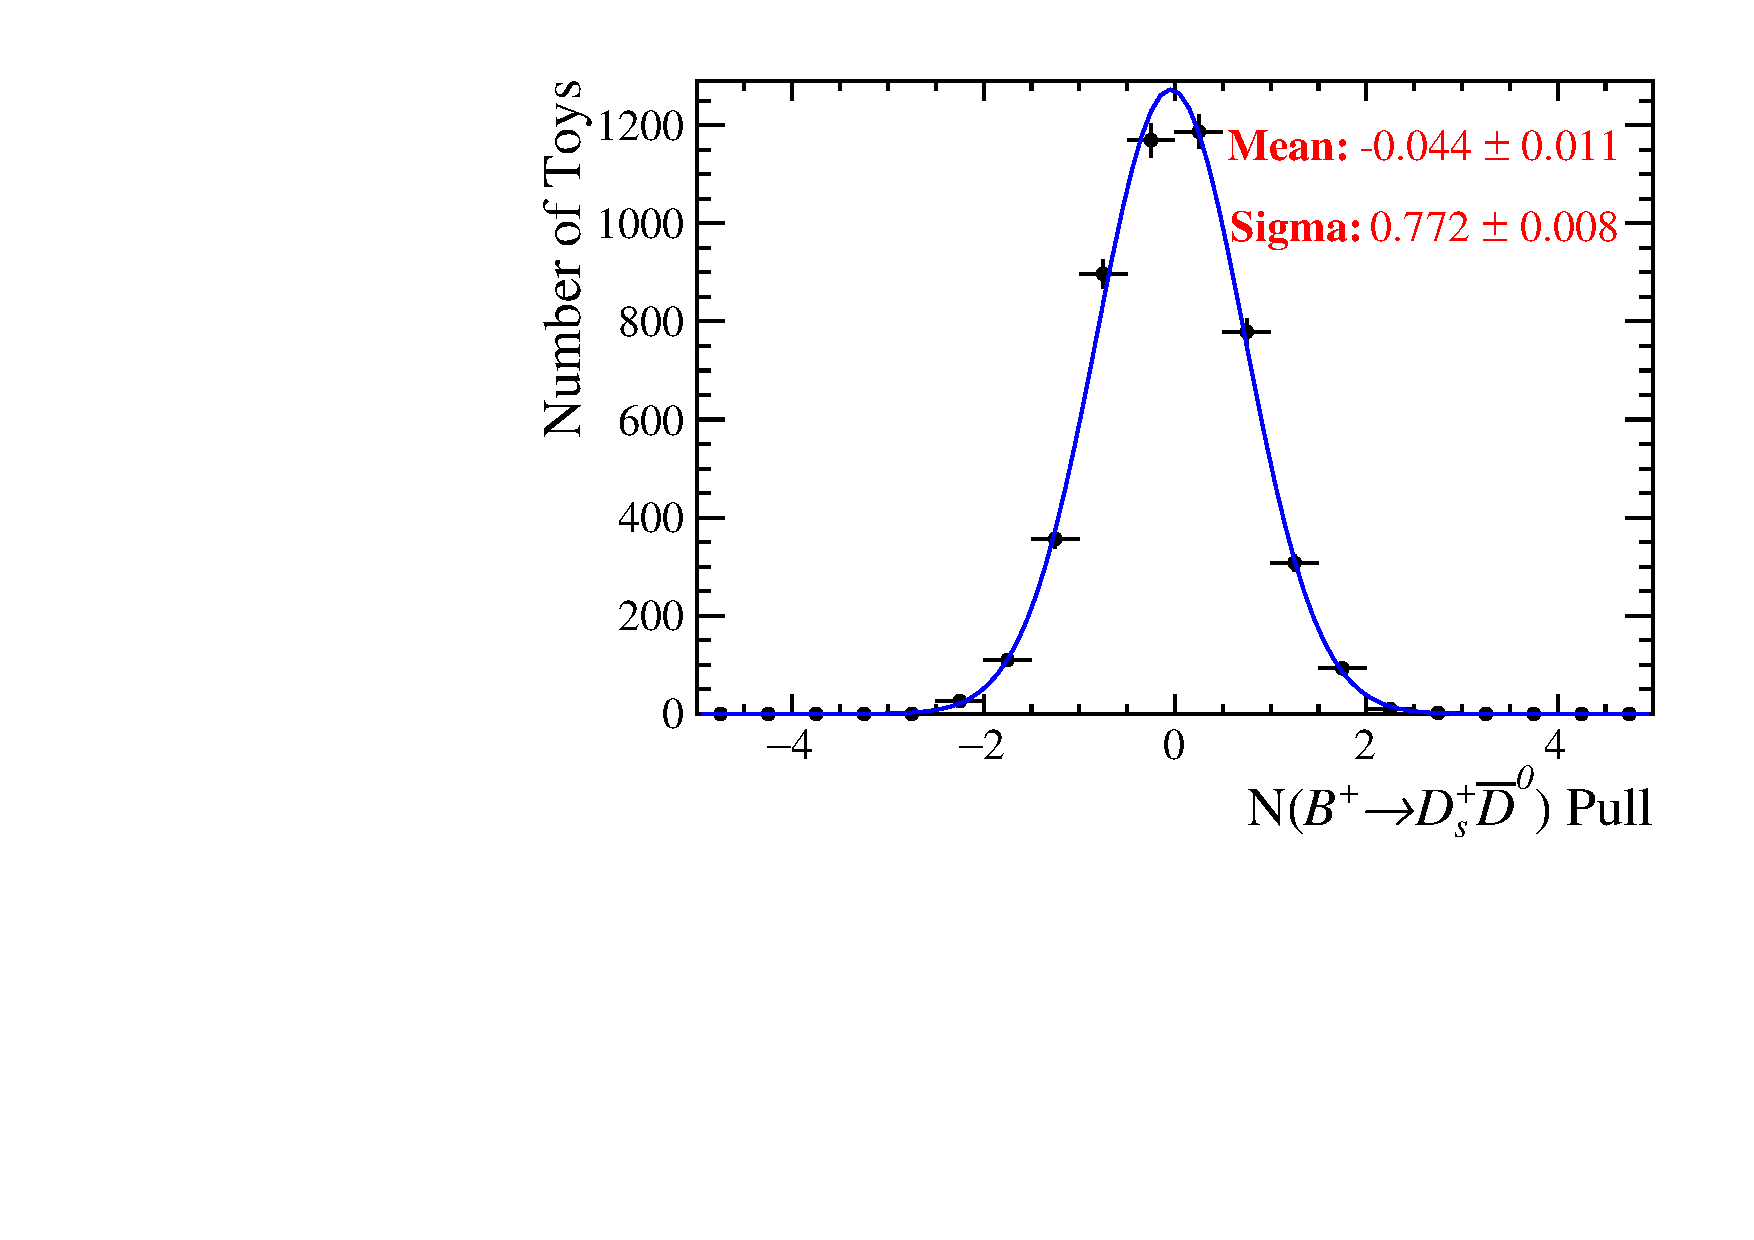
\includegraphics[width=0.32\textwidth]{figs/B2DsKK/Plots_DsD0_nsig_pul.pdf}
%       \caption{Normalisation fit}
%    \end{subfigure}\\
%    \caption{The distribution of the signal and normalisation yields, errors and pulls as determined from pseudo-experiments. The result of fit performed to the pull distributions is overlaid in blue, along with the numerical results in red.}
%    \label{fig:B2DsKK_Pulls}
% \end{figure}
% %%%%%%%%%%%%%%%%%%%%%%%%%%%%%%%%%%%%%%%%%%%%%%%%%%%%%%%%%%

% The distributions of the yields, errors and pulls for the signal and normalisation pseudo-experiments are shown in Fig.~\ref{fig:B2DsKK_Pulls}. A fit is performed for each pull distributions using a Gaussian to determine the mean and width. 
% For the signal yield the mean and with are within $3\sigma$ of zero and one respectively. The normalisation yield shows a significant bias in the width. The bias implies the fit model is overestimating the uncertainty $\sigma$ of the yield.
% If the normalisation yield uncertainty dominates the uncertainty in the branching fraction this could lead to an overestimation of the uncertainty on the final measured branching fraction.

% To determine how the normalisation uncertainty propagates to the branching fraction another set of pseudo-experiments are produced.
% This set includes both signal and normalisation decays. To calculated the branching fraction the yield of \decay{\Bp}{\Dsp\Kp\Km} decays is corrected according to the signal efficiency as a function of the kinematics of a given candidate, as detailed previously in Eq.~\ref{eq:B2DsKK_corrected_yield}. The candidates are assumed to have a flat distribution in the two dimensional $m^{2}(\Kp\Km)$ vs. $m^{2}(\Dsp\Km)$ space used to parametrise the efficiency. The bias in the final branching fraction is much smaller than the bias normalisation pull.



%%%%%%%%
% For each pseudo-experiment the branching fraction and uncertainty are produced. As no branching fraction is explicitly used to generate the pseudo-experiment (rather independent signal and normalisation yields), the pulls are redefined to be measured relative to the mean branching fraction
% \begin{equation}
% g_{\text{pull}} = \frac{x_{\text{fit}} - \bar{x}_{\text{fit}} }{\sigma}
% \end{equation}
% where $x_{\text{fit}}$ is the fitted value of the parameter, $\bar{x}_{\text{fit}}$ is the average of all fitted values and $\sigma$ is the uncertainty. The distribution of the branching fraction, uncertainty and pull are shown in Fig~\ref{fig:B2DsKK_BR_Pulls}. 


% %%%%%%%%%%%%%%%%%%%%%%%%%%%%%%%%%%%%%%%%%%%%%%%%%%%%%%%%%%
% \begin{figure}[!h]
%    \centering
%    \begin{subfigure}[t]{1.0\textwidth}
%       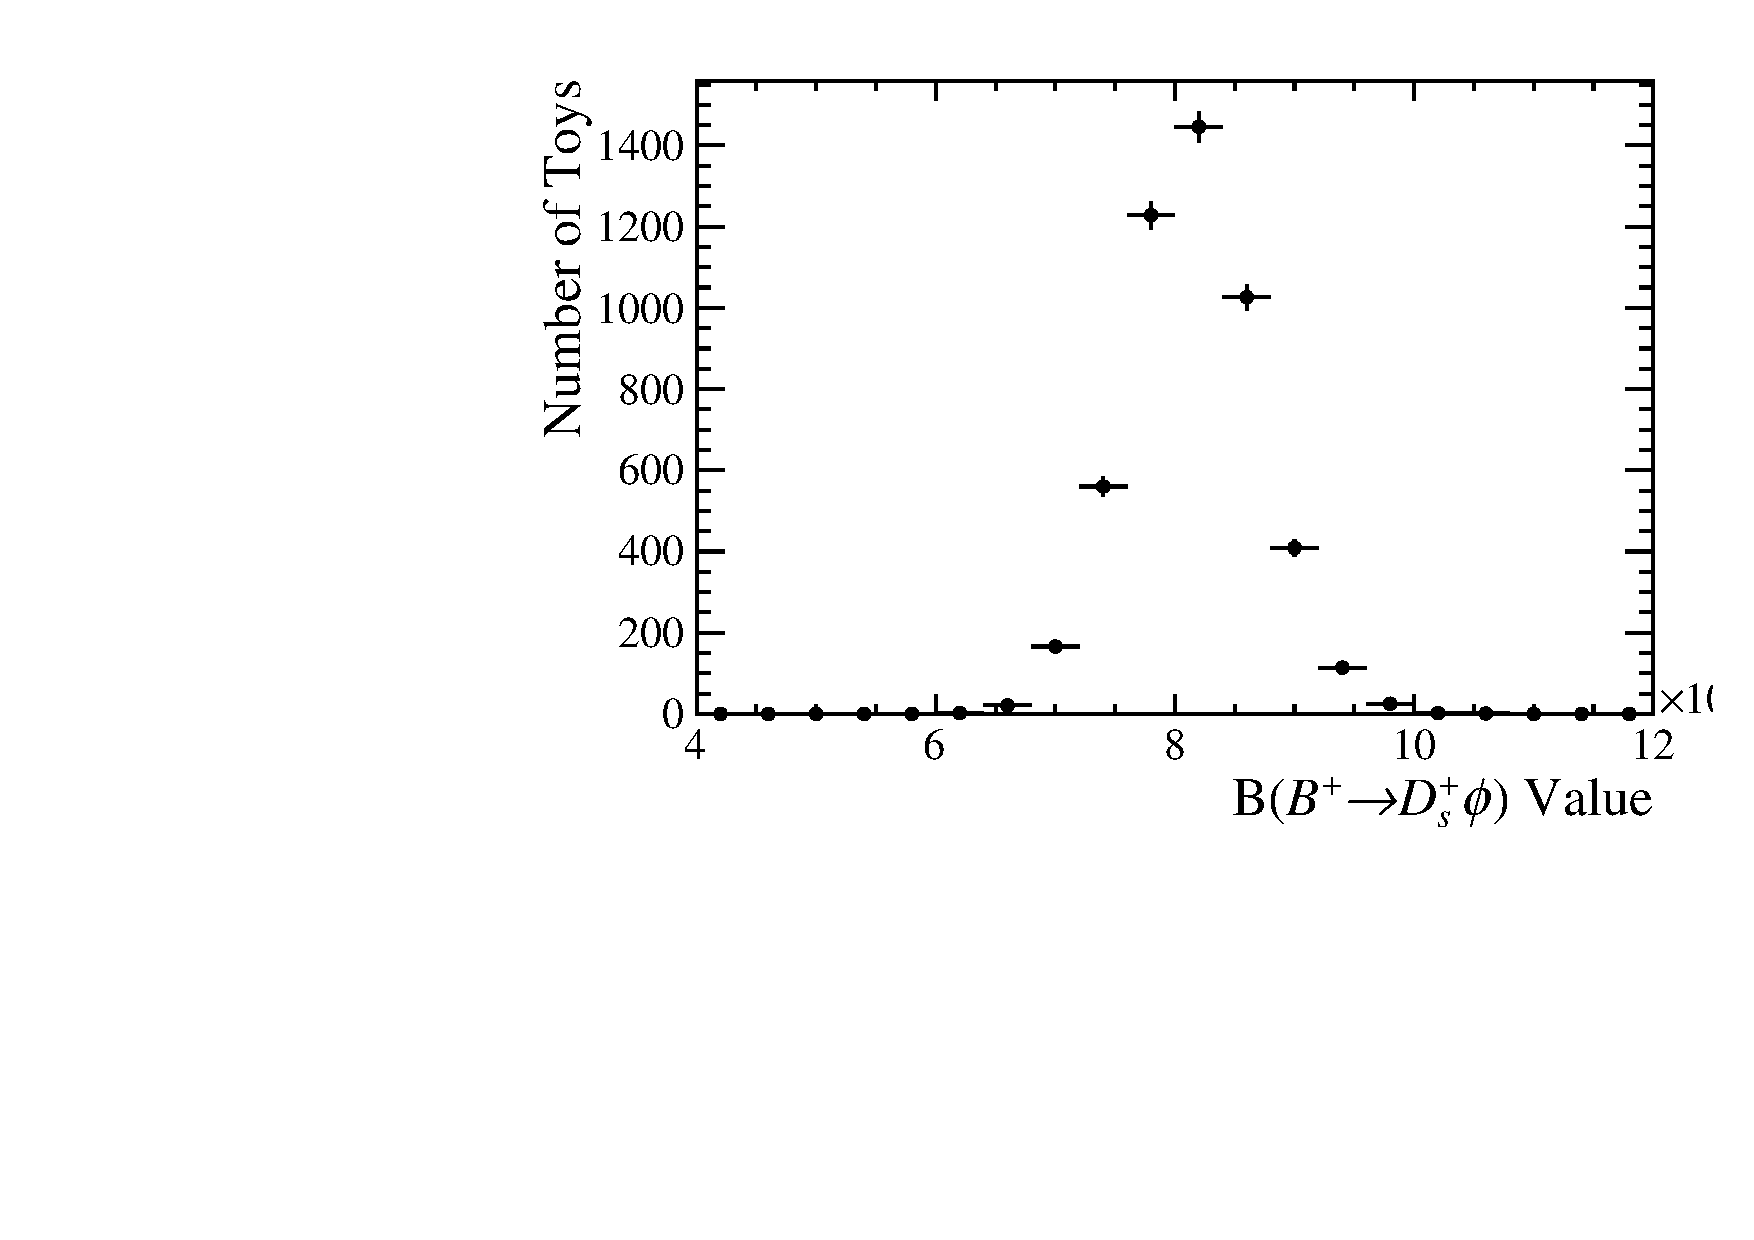
\includegraphics[width=0.32\textwidth]{figs/B2DsKK/Branching_Fraction_val.pdf}
%       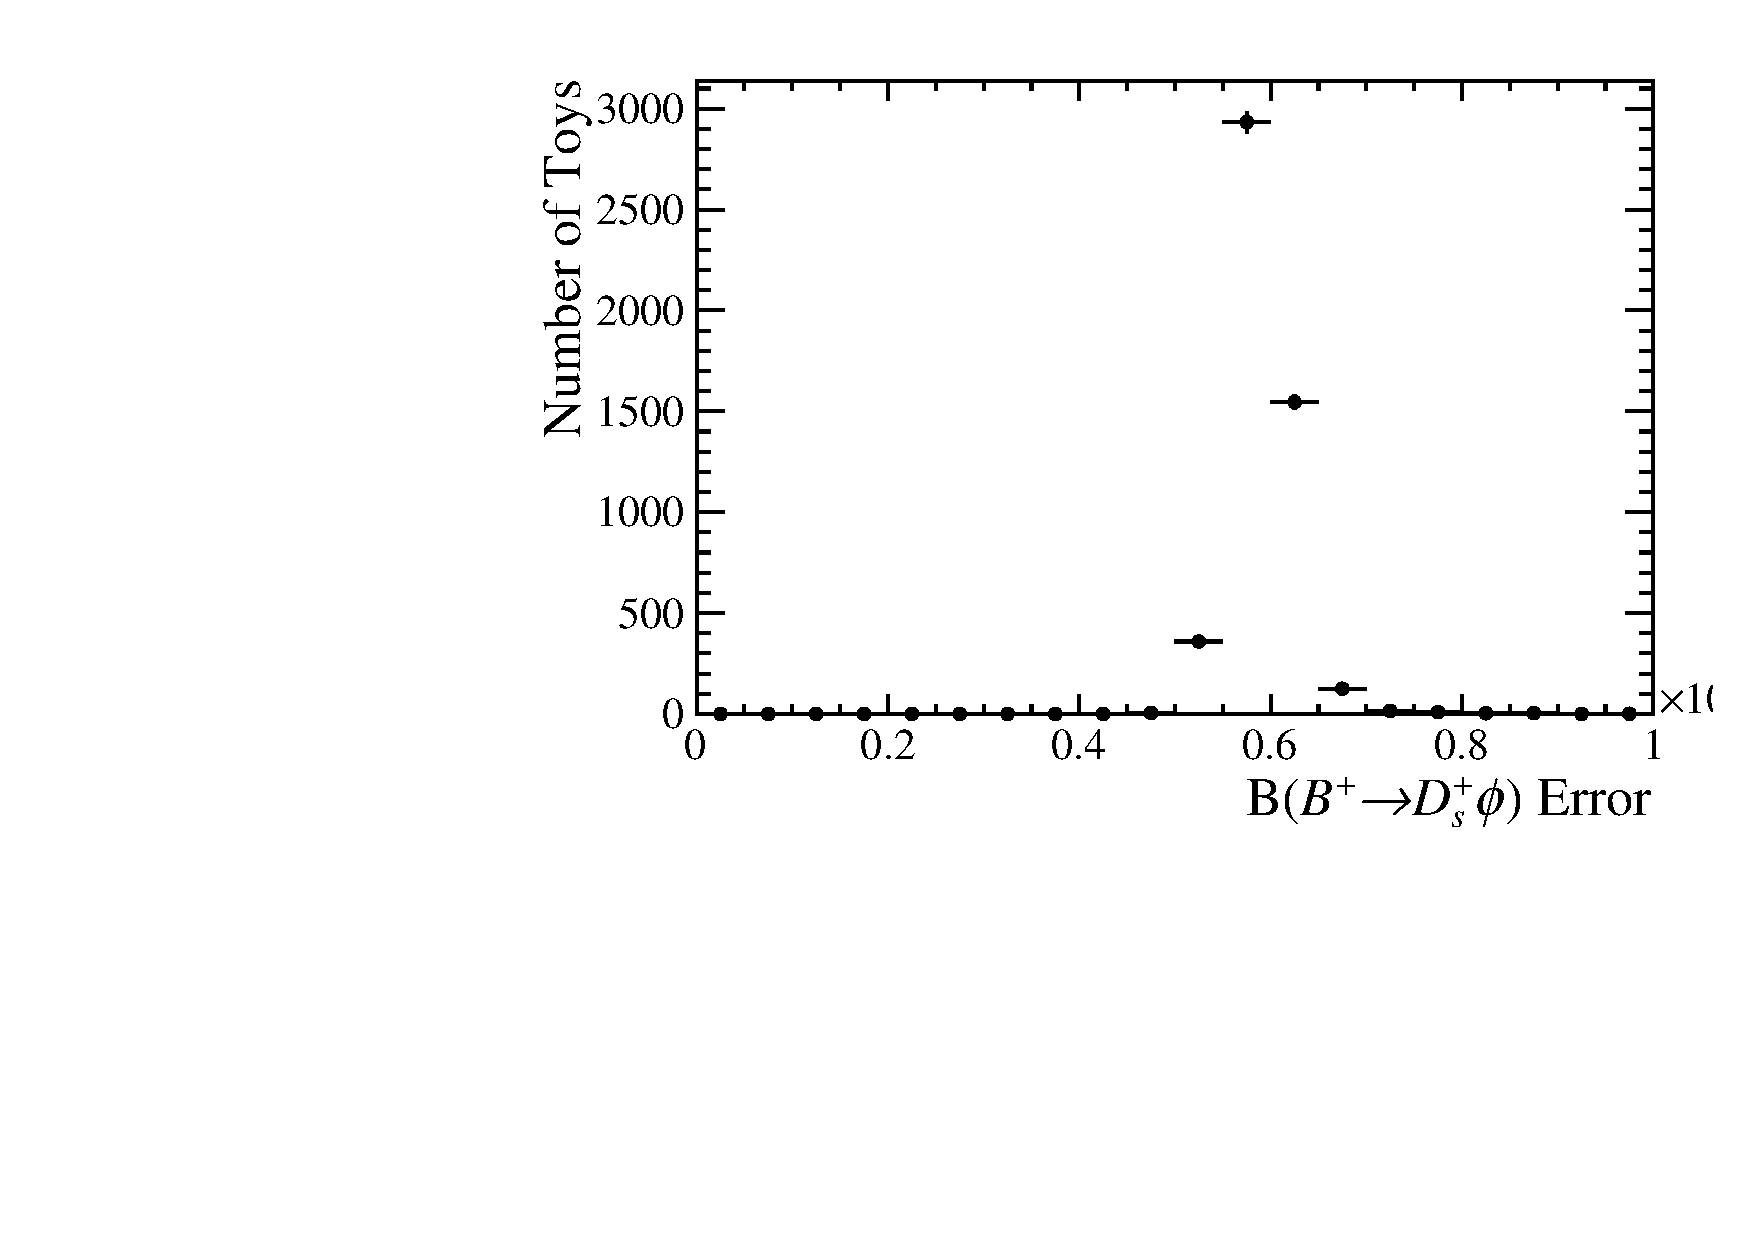
\includegraphics[width=0.32\textwidth]{figs/B2DsKK/Branching_Fraction_err.pdf}
%       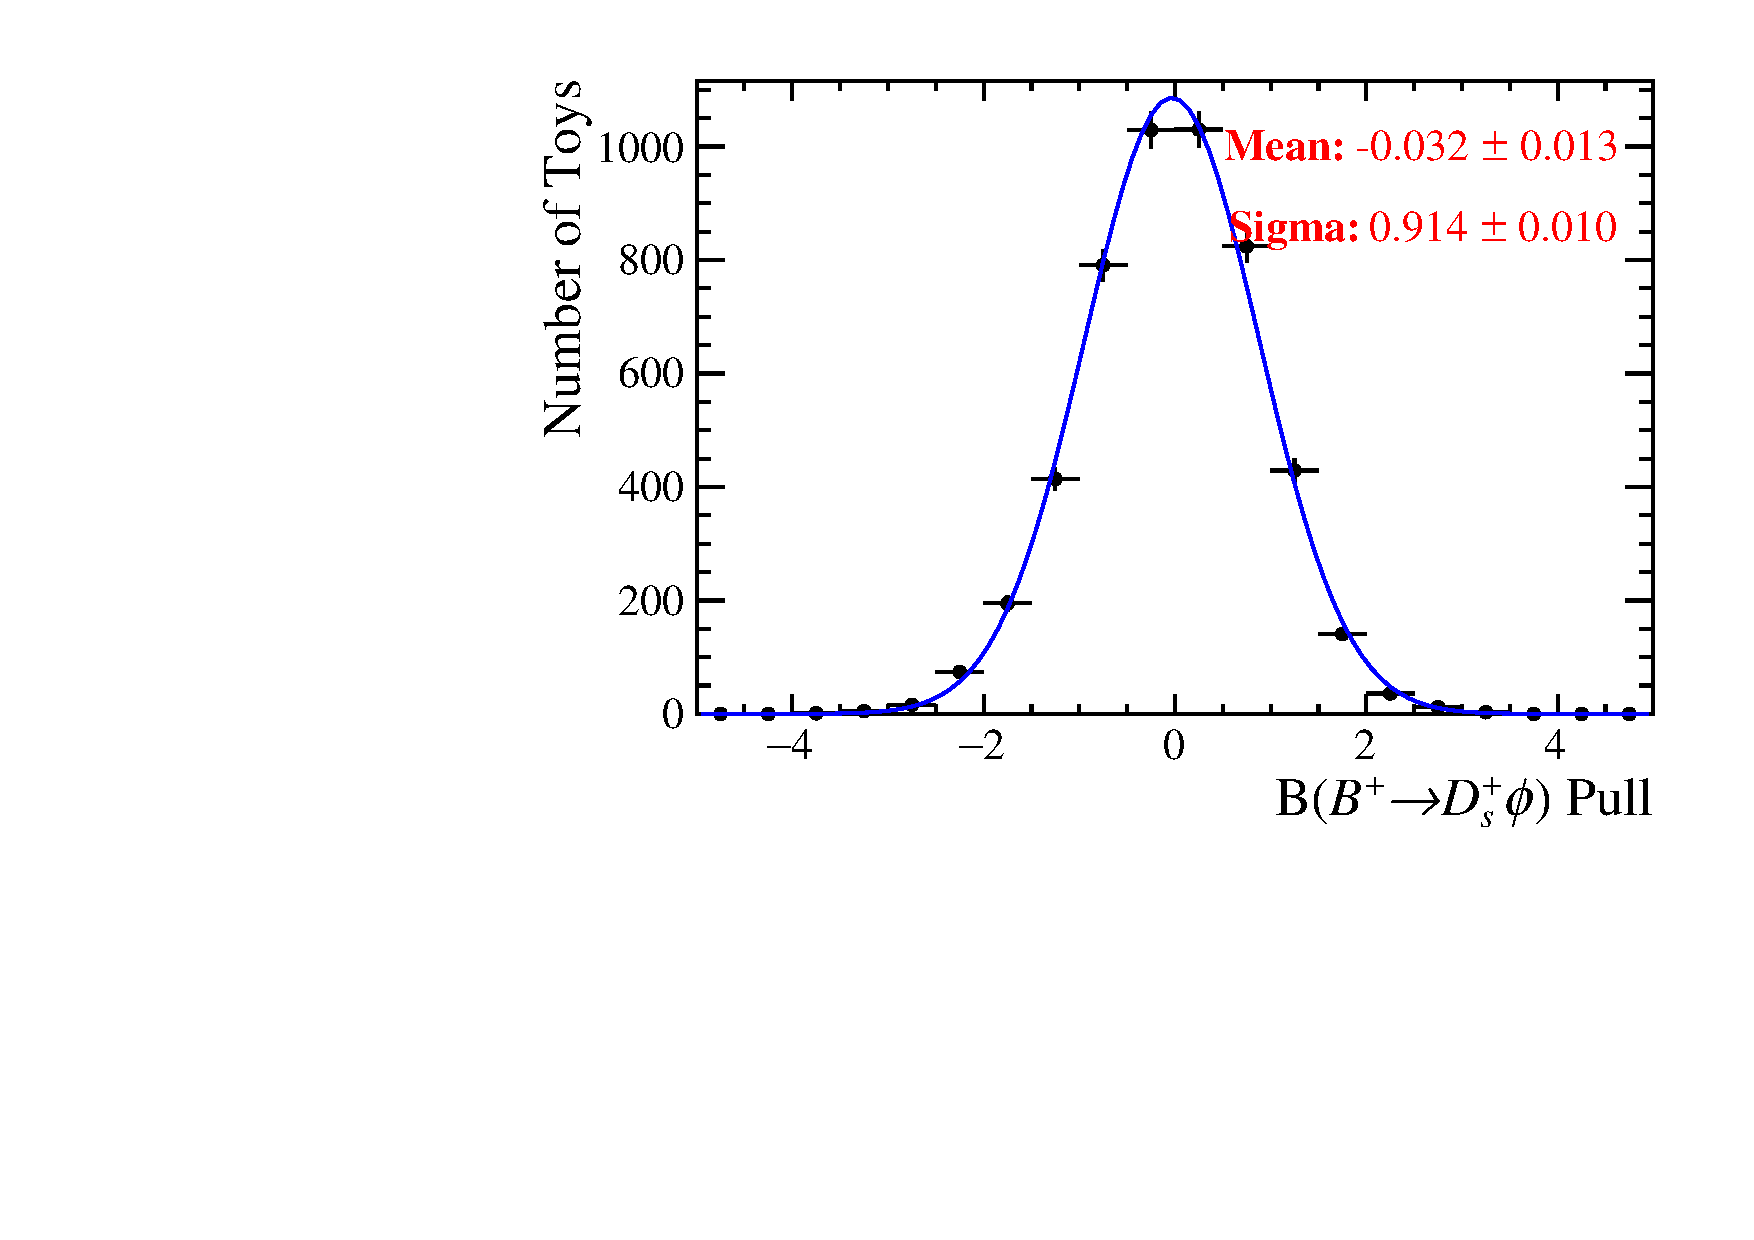
\includegraphics[width=0.32\textwidth]{figs/B2DsKK/Branching_Fraction_pul.pdf}
%    \end{subfigure}\\
%    \caption{The distribution of the branching fraction, error and pull as determined from pseudo-experiments. The result of fit performed to the pull distributions is overlaid in blue, along with the numerical results in red.}
%    \label{fig:B2DsKK_BR_Pulls}
% \end{figure}
% %%%%%%%%%%%%%%%%%%%%%%%%%%%%%%%%%%%%%%%%%%%%%%%%%%%%%%%%%%

% The pull in the branching fraction has a much smaller bias in the width than the normalisation pull.
% It would be possible to scale the uncertainty in the branching fraction as determined by the fit to account for the residual bias in the uncertainty. However, this would introduce a source of systematic uncertainty associated to scaling factor so the choice is made to not correct the slightly overestimated uncertainty. 

\section{Normalisation and signal fits}

The signal and normalisation fits are performed using the model and data set previously described. The results of the two fits are shown in Figs.~\ref{fig:B2DsKK_fit_B2DsD0} and \ref{fig:B2DsKK_fit_B2DsKK}. These figures show the distribution of \Bp candidates along with the total model PDF constructed with the values of the free parameters determined in the negative log likelihood minimisation process. The contributions from each different component in the model are superimposed, stacked upon one another, and detailed in the legends.

%%%%%%%%%%%%%%%%%%%%%%%%%%%%%%%%%%%%%%%%%%%%%%%%%%%%%%%%%%
\begin{figure}[!h]
    \centering
    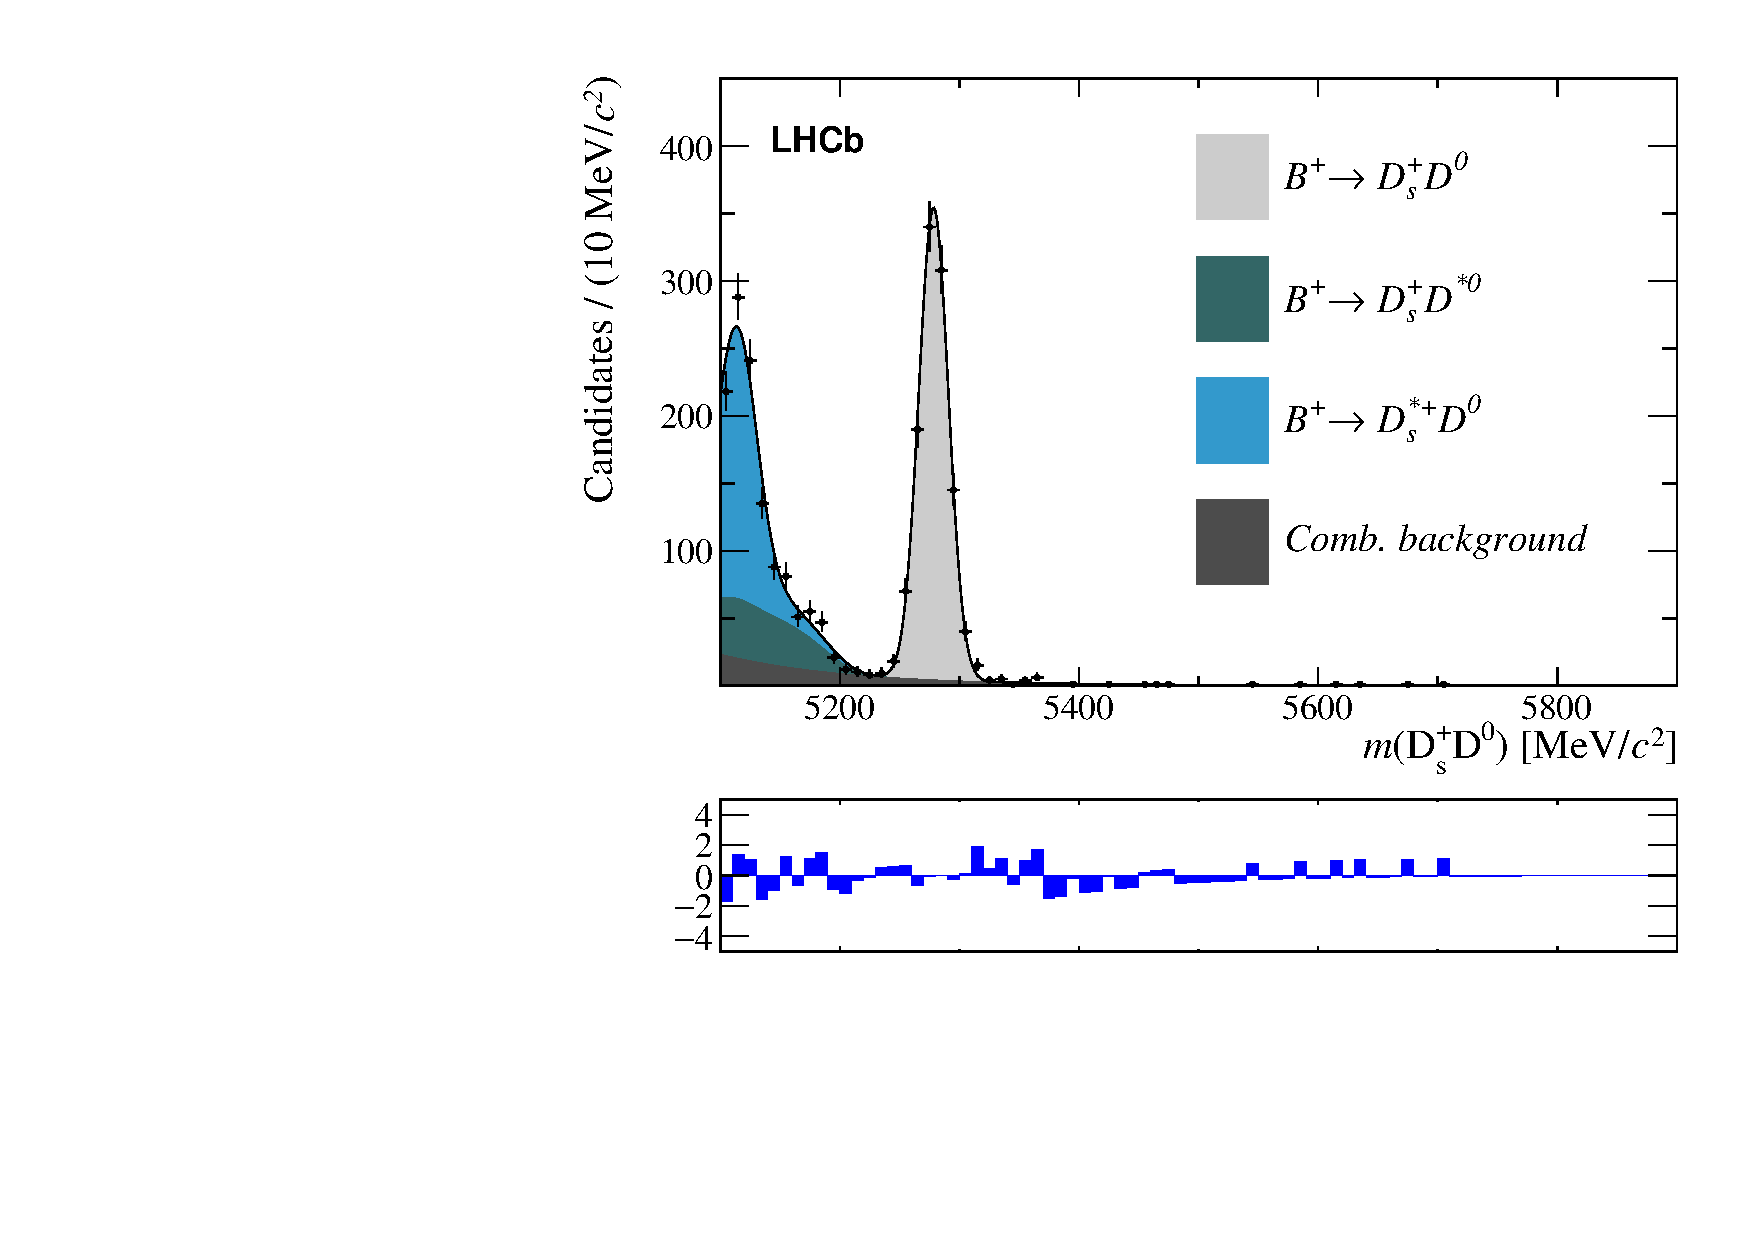
\includegraphics[width=0.8\textwidth]{figs/B2DsKK/Fit_DsD0.pdf}
    \caption{Invariant mass fit to \decay{\Bp}{\Dsp\Dzb} candidates.}
    \label{fig:B2DsKK_fit_B2DsD0}   
\end{figure}
%%%%%%%%%%%%%%%%%%%%%%%%%%%%%%%%%%%%%%%%%%%%%%%%%%%%%%%%%%
%%%%%%%%%%%%%%%%%%%%%%%%%%%%%%%%%%%%%%%%%%%%%%%%%%%%%%%%%%
\begin{figure}[!h]
    \centering
    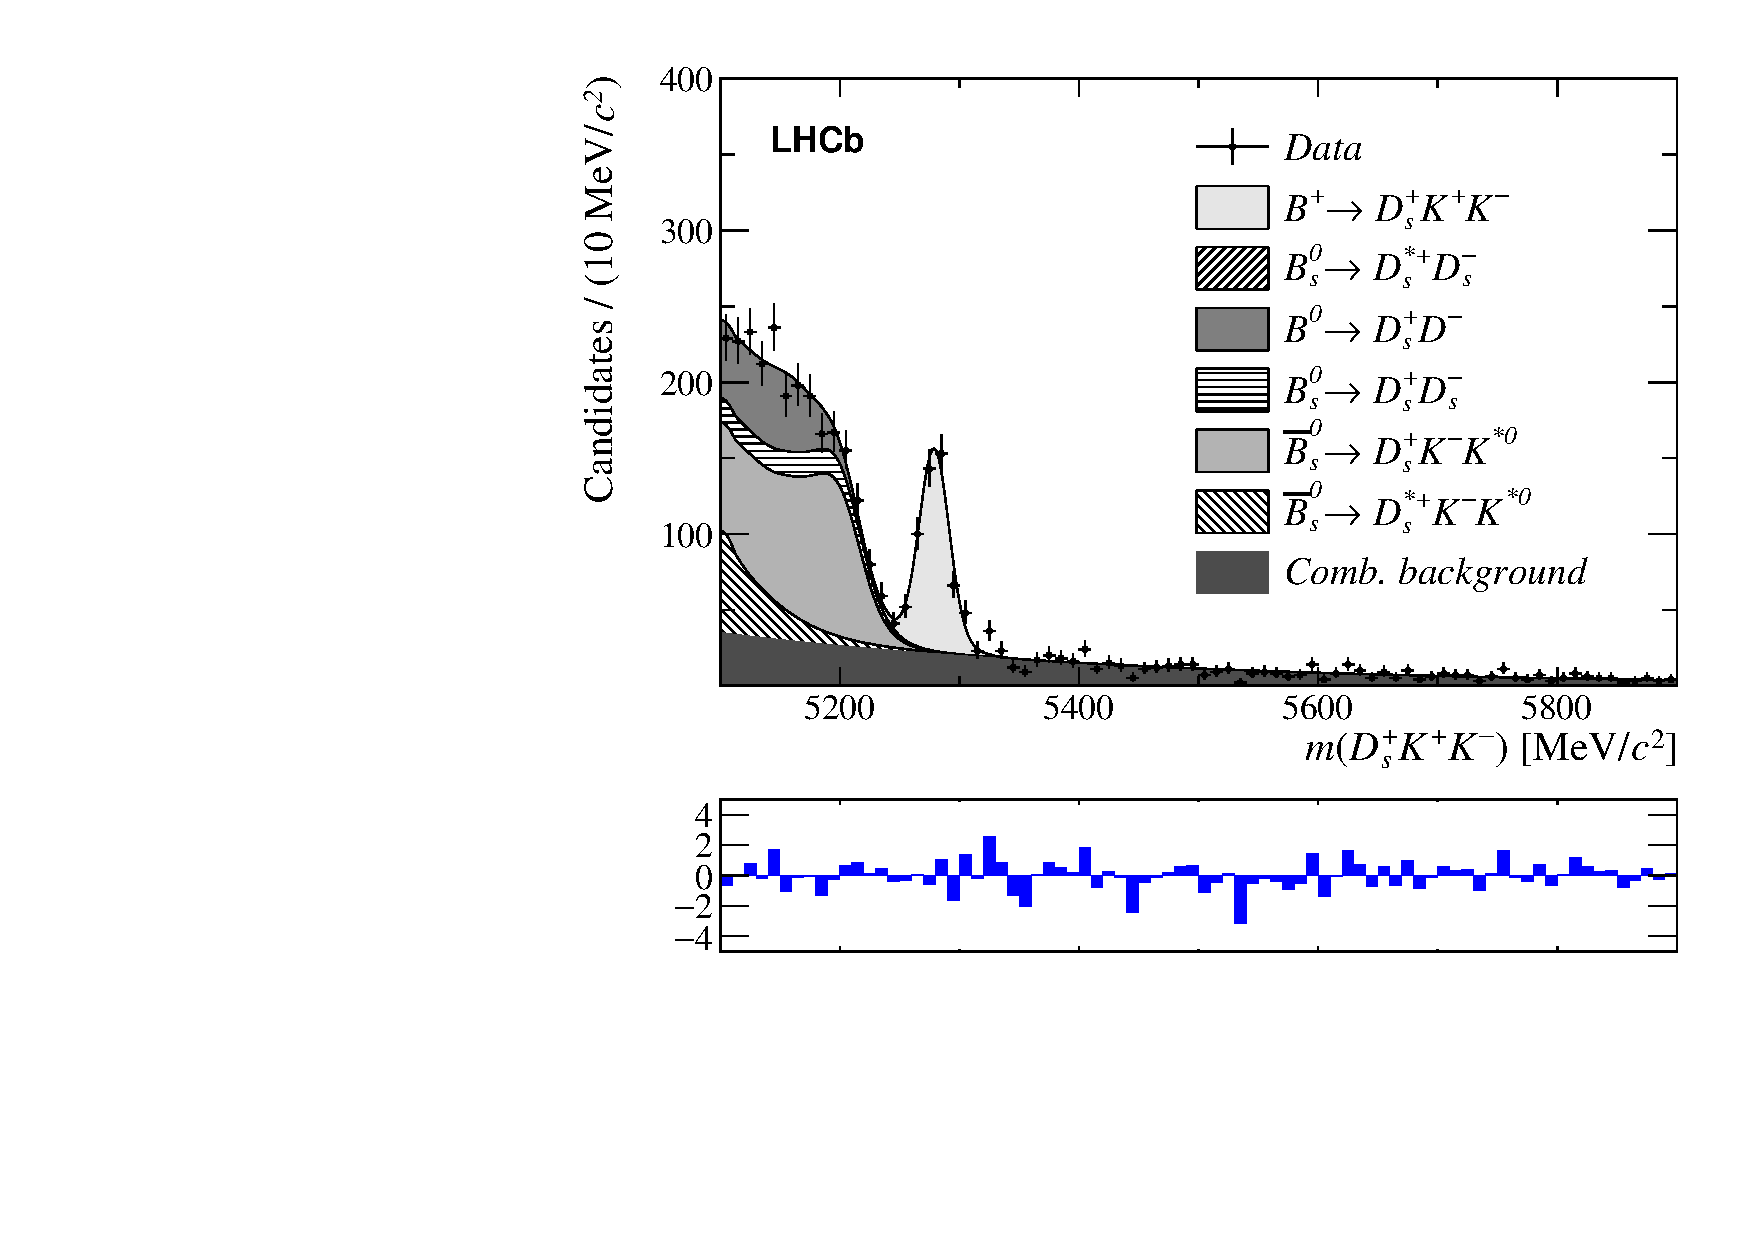
\includegraphics[width=0.8\textwidth]{figs/B2DsKK/Fit_DsKK.pdf}
    \caption{Invariant mass fit to \decay{\Bp}{\Dsp\Kp\Km} candidates.}
    \label{fig:B2DsKK_fit_B2DsKK}   
\end{figure}
%%%%%%%%%%%%%%%%%%%%%%%%%%%%%%%%%%%%%%%%%%%%%%%%%%%%%%%%%%

The distribution of \decay{\Bp}{\Dsp\Dzb} candidates in Fig.~\ref{fig:B2DsKK_fit_B2DsD0} demonstrates the relatively high purity of the selection. Additionally, there is a good separation between the normalisation peak and the partially reconstructed background. Only the combinatorial background is found to have a contribution at the same invariant mass as the normalisation peak. 


The distribution of \decay{\Bp}{\Dsp\Kp\Km} candidates shown in Fig.~\ref{fig:B2DsKK_fit_B2DsKK} has a significant contribution from the signal decay. The background contribution under the signal PDF is larger than was observed for the normalisation channel. Although the dominant background below the signal is still the combinatorial background, the contribution from the partially reconstructed backgrounds is also larger; several of the background PDFs extend underneath the leftmost half of the signal distribution.  


The numerical values of the free parameters determined in the fit to the signal and normalisation channels are listed in Tables~\ref{tab:B2DsKK_fit_result_norm} and \ref{tab:B2DsKK_fit_result_signal}.

\begin{table}[h]
    \centering
    \begin{tabular}{ l l S[table-format=4.1(3)] }
        \hline
        Type       & Parameter                                 & {Fit result}                         \\
        \hline
        POI         & $N(\decay{\Bp}{\Dsp\Dzb})$               & 1091\pm34                \\

                  %         nsig    1.0905e+03    1.0905e+03 +/-  3.42e+01  <none>
        \hline
        Shape       & Mass shift $\delta$ (\mevcc)              & -10.6\pm1.3                 \\
                    & Relative peak heights $\xi$               & 0.0\pm0.2                       \\
                    & Mean \Bp mass $\mu$ (\mevcc)              & 5278.4\pm0.4                    \\
                    & Signal width $\sigma_{1}$ (\mevcc)        & 12.4\pm0.3                      \\
                    & Combinatorial slope $c$                   & -9.4\pm1.1$\times10^{-3}$     \\
                  %   global_csi    1.2683e-06    5.2233e-08 +/-  2.25e-01  <none>
                  % global_shift   -1.0585e+01   -1.0586e+01 +/-  1.31e+00  <none>
                  %       mean_B    5.2784e+03    5.2784e+03 +/-  4.00e-01  <none>
                  %        slope   -9.4305e-03   -9.4308e-03 +/-  1.13e-03  <none>
                  %        sigma    1.2436e+01    1.2435e+01 +/-  3.23e-01  <none>
        \hline
        Yields      & $N_{\text{comb}}$                         & 248\pm54                        \\
                    & $N(\decay{\Bp}{\Dsp\Dstarzb})$            & 331\pm67                        \\
                    & $N(\decay{\Bp}{\Dssp\Dzb})$               & 752\pm55                        \\
                  %          nBG    2.4773e+02    2.4769e+02 +/-  5.42e+01  <none>
                  %      nDsDst0    3.3055e+02    3.3055e+02 +/-  6.72e+01  <none>
                  %      nDsstD0    7.5230e+02    7.5220e+02 +/-  5.48e+01  <none>
        \hline
    \end{tabular}  
    \caption{Normalisation fit result. } 
    \label{tab:B2DsKK_fit_result_norm}
\end{table}
  

\begin{table}[h]
    \centering
    \begin{tabular}{ l l S[table-format=4.1(3)] }

        \hline
        Type        & Parameter                                 & {Fit result}                    \\
        \hline
        POI         & $N(\decay{\Bp}{\Dsp\Kp\Km})$              & 442\pm29                    \\
                  %         nsig    4.4287e+02    4.4277e+02 +/-  2.94e+01  <none>
        \hline
        Shape       & Mass shift $\delta$ (\mevcc)              & 4\pm12                      \\
                    & Mean \Bp mass $\mu$ (\mevcc)              & 5278.9\pm0.9                \\
                    & Signal width $\sigma_{1}$ (\mevcc)        & 12.3\pm0.9                  \\
                    & Combinatorial slope $c$                   & -2.8\pm0.3$\times 10^{-3}$ \\
                  % global_shift    2.2538e+00    3.5457e+00 +/-  1.17e+01  <none>
                  %       mean_B    5.2789e+03    5.2789e+03 +/-  8.82e-01  <none>
                  %        sigma    1.2298e+01    1.2291e+01 +/-  8.77e-01  <none>
                  %        slope   -2.8199e-03   -2.8202e-03 +/-  2.79e-04  <none>
        \hline
        Yields      & $N_{\text{comb}}$                         & 1114\pm73                   \\
                    & $N(\decay{\Bsb}{\Dsp\Km\Kstarz})$         & 1115\pm461                  \\
                    & $N(\decay{\Bsb}{\Dssp\Km\Kstarz})$        & 297\pm124                   \\
                    & $N(\decay{\Bs}{\Dsp\Dsm})$                & 203\pm508                   \\
                    & $N(\decay{\Bz}{\Dsp\Dm})$                 & 466\pm154                   \\
                    & $N(\decay{\Bs}{\Dssp\Dsm})$               & 0\pm398                     \\
                  %          nBG    1.1139e+03    1.1142e+03 +/-  7.30e+01  <none>
                  %     nBs2Dsa1    1.1153e+03    1.1147e+03 +/-  4.61e+02  <none>
                  % nBs2DsstKKst    2.9756e+02    2.9691e+02 +/-  1.24e+02  <none>
                  %     nBs2DsDs    2.0262e+02    2.0307e+02 +/-  5.08e+02  <none>
                  %      nB02DsD    4.6587e+02    4.6621e+02 +/-  1.54e+02  <none>
                  %   nBs2DsstDs    1.1208e-04    6.2385e-02 +/-  3.98e+02  <none>
        \hline
    \end{tabular}  
    \caption{Signal fit result.} 
    \label{tab:B2DsKK_fit_result_signal}
\end{table}



Two of the common parameters between the two modes, namely the mean \Bp mass and width, have consistent values between the two fits. The combinatorial slopes vary between the two, likely because of the different background levels in the two datasets. Similarly the mass shifts vary between the two, but are consistent within the quoted uncertainties. 

\section{Efficiency corrections}
\label{sec:B2DsKK_effcorrection}

The branching fraction for \decay{\Bp}{\Dsp\Kp\Km} decays is determined by correcting the yields of signal and background decays by their corresponding selection efficiencies. 
%These account for each step of the selection process and ultimately quantifies the extent to which the signal and normalisation channels are affected differently. 
The signal yield is corrected by the efficiency as a function of the candidate's kinematic properties. The relative signal efficiency is determined as a function of the two-dimensional Dalitz plot coordinates $m^{2}(\Dsp\Km)$ and $m^{2}(\Kp\Km)$
\begin{equation}
\epsilon_{\text{ratio}}(m^{2}(\Dsp\Km),m^{2}(\Kp\Km)) = \frac{\epsilon_{\decay{\Bp}{\Dsp\Kp\Km}}(m^{2}(\Dsp\Km),m^{2}(\Kp\Km))}{\epsilon_{\decay{\Bp}{\Dsp\Dzb}}}.
\end{equation}
The normalisation decay efficiency $\epsilon_{\decay{\Bp}{\Dsp\Dzb}}$ is a pseudo-two-body decay and therefore the efficiency has no dependence on the phase-space coordinates. 
%The kinematic phase-space is split into bins and the efficiencies determined in each. 

The efficiencies are determined using simulated decays. The PID and MVA efficiencies require additional input from external calibration samples.

\subsection{Efficiencies from simulations only} 


\subsubsection{Acceptance}
The relative likelihood for the five signal or normalisation tracks to be within the \lhcb detector's acceptance, $10 < \cos\theta < 400 \mrad$, is shown as a function of the \decay{\Bp}{\Dsp\Kp\Km} Dalitz plot in Fig.\ref{fig:B2DsKK_releff_acceptance}.

\subsubsection{Reconstruction} 
The relative reconstruction efficiency shown in Fig.~\ref{fig:B2DsKK_releff_reconstruction} accounts for the fraction of decays in which the candidate has been correctly reconstructed and passes the \decay{\Bp}{\Dsp\Kp\Km} \emph{Stripping Line} requirements. Only events with a positive trigger decision are reconstructed (in simulation and data). The \decay{\Bp}{\Dsp\Dzb} normalisation decays are reconstructed using the \decay{\Bp}{\Dsp\Kp\Km} topology. This requires the \Dsp, \Kp and \Km candidates to form a well reconstructed vertex, reducing the efficiency for long-lived \Dzb mesons. 

\subsubsection{Trigger} 
The relative trigger efficiency shown in Fig.~\ref{fig:B2DsKK_releff_trigger} accounts for the fraction of decays for which the signal candidate meets the \texttt{TIS} and \texttt{TOS} requirements, given that there was a positive trigger decision in that event, typically around 95\%. 

\subsubsection{Vetoes} 
The relative veto efficiency shown in Fig.~\ref{fig:B2DsKK_releff_vetoes} accounts for the fraction of decays passing the invariant mass and normalisation vetoes. The vetoes to remove misidentified \D and \Lc hadrons are only applied to the \Dsp meson and therefore assumed to affect the signal and normalisation mode equally.
A vertical band is clear in the centre as a result of the veto for misidentified normalisation decays with \decay{\Dzb}{\Kp\pim}.

\subsubsection{Charmless} 
The relative charmless efficiency shown in Fig.\ref{fig:B2DsKK_releff_charmless} accounts for the fraction of decays failing the requirements on the \D meson flight distance requirements aimed at removing charmless and single-charm backgrounds.

\subsubsection{Impact parameter significance} 
The relative $\chi^{2}_{\text{IP}}$ efficiency shown in Fig.~\ref{fig:B2DsKK_releff_ipchi2} accounts for the fraction of decays that pass the requirements on the \Bp and \Dsp meson impact parameter significance. The distribution shows a strong dependency on the position in phase-space at high $m^{2}(\Kp\Km)$ which may be because the \Dsp mesons are produced collinear with the \Bp direction and fail the minimum impact parameter significance requirement.

\subsubsection{Mass windows} 
The relative mass requirements efficiency shown in Fig.~\ref{fig:B2DsKK_releff_masswindows} accounts for the fraction of decays that pass the mass windows around the \Dsp (and \Dzb) mass. 


%%%%%%%%%%%%%%%%%%%%%%%%%%%%%%%%%%%%%%%%%%%%%%%%%%%%%%%%%%
\begin{figure}[!h]
    \centering
    \begin{subfigure}[t]{0.40\textwidth}
        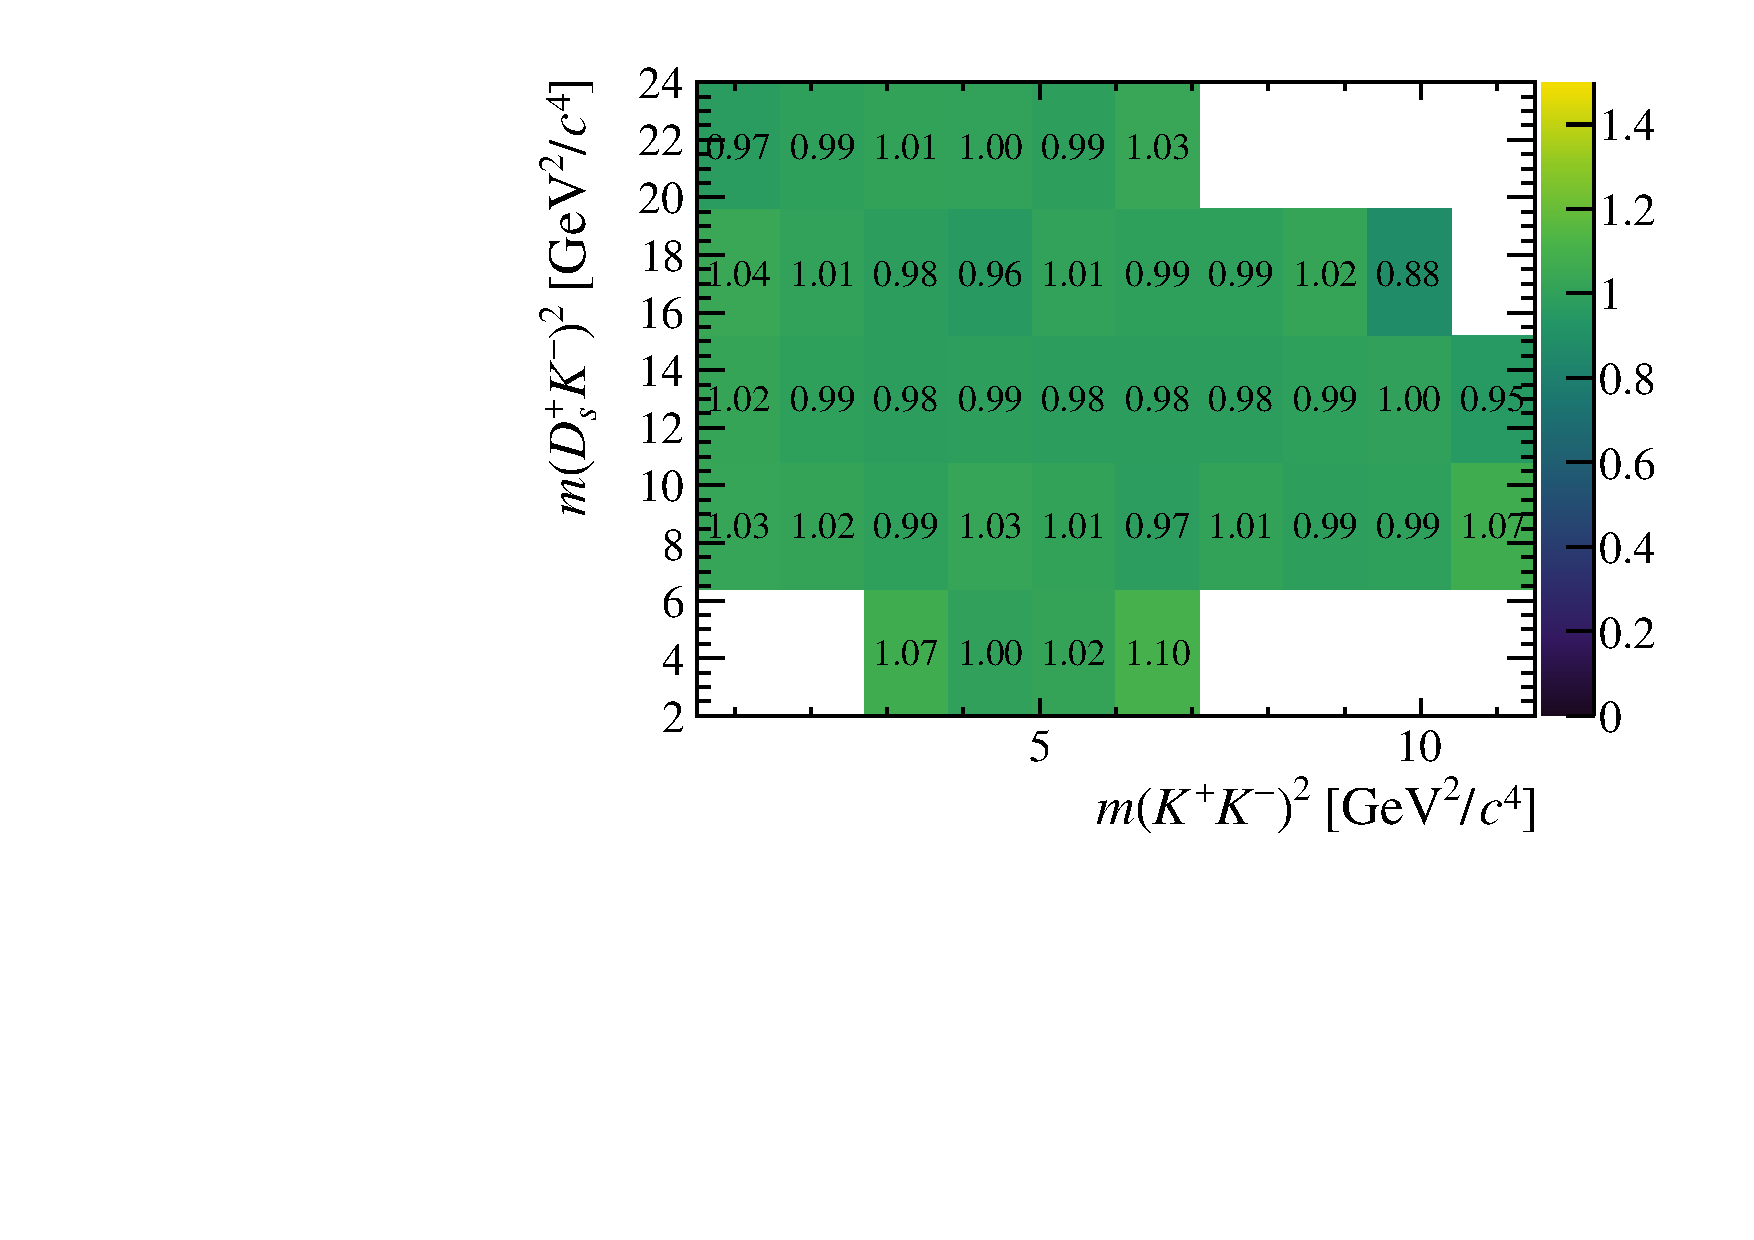
\includegraphics[width=1.0\textwidth]{figs/B2DsKK/Relative_Eff_gen_All_Full.pdf}
        \caption{Acceptance}
        \label{fig:B2DsKK_releff_acceptance}
    \end{subfigure}
    \begin{subfigure}[t]{0.40\textwidth}
        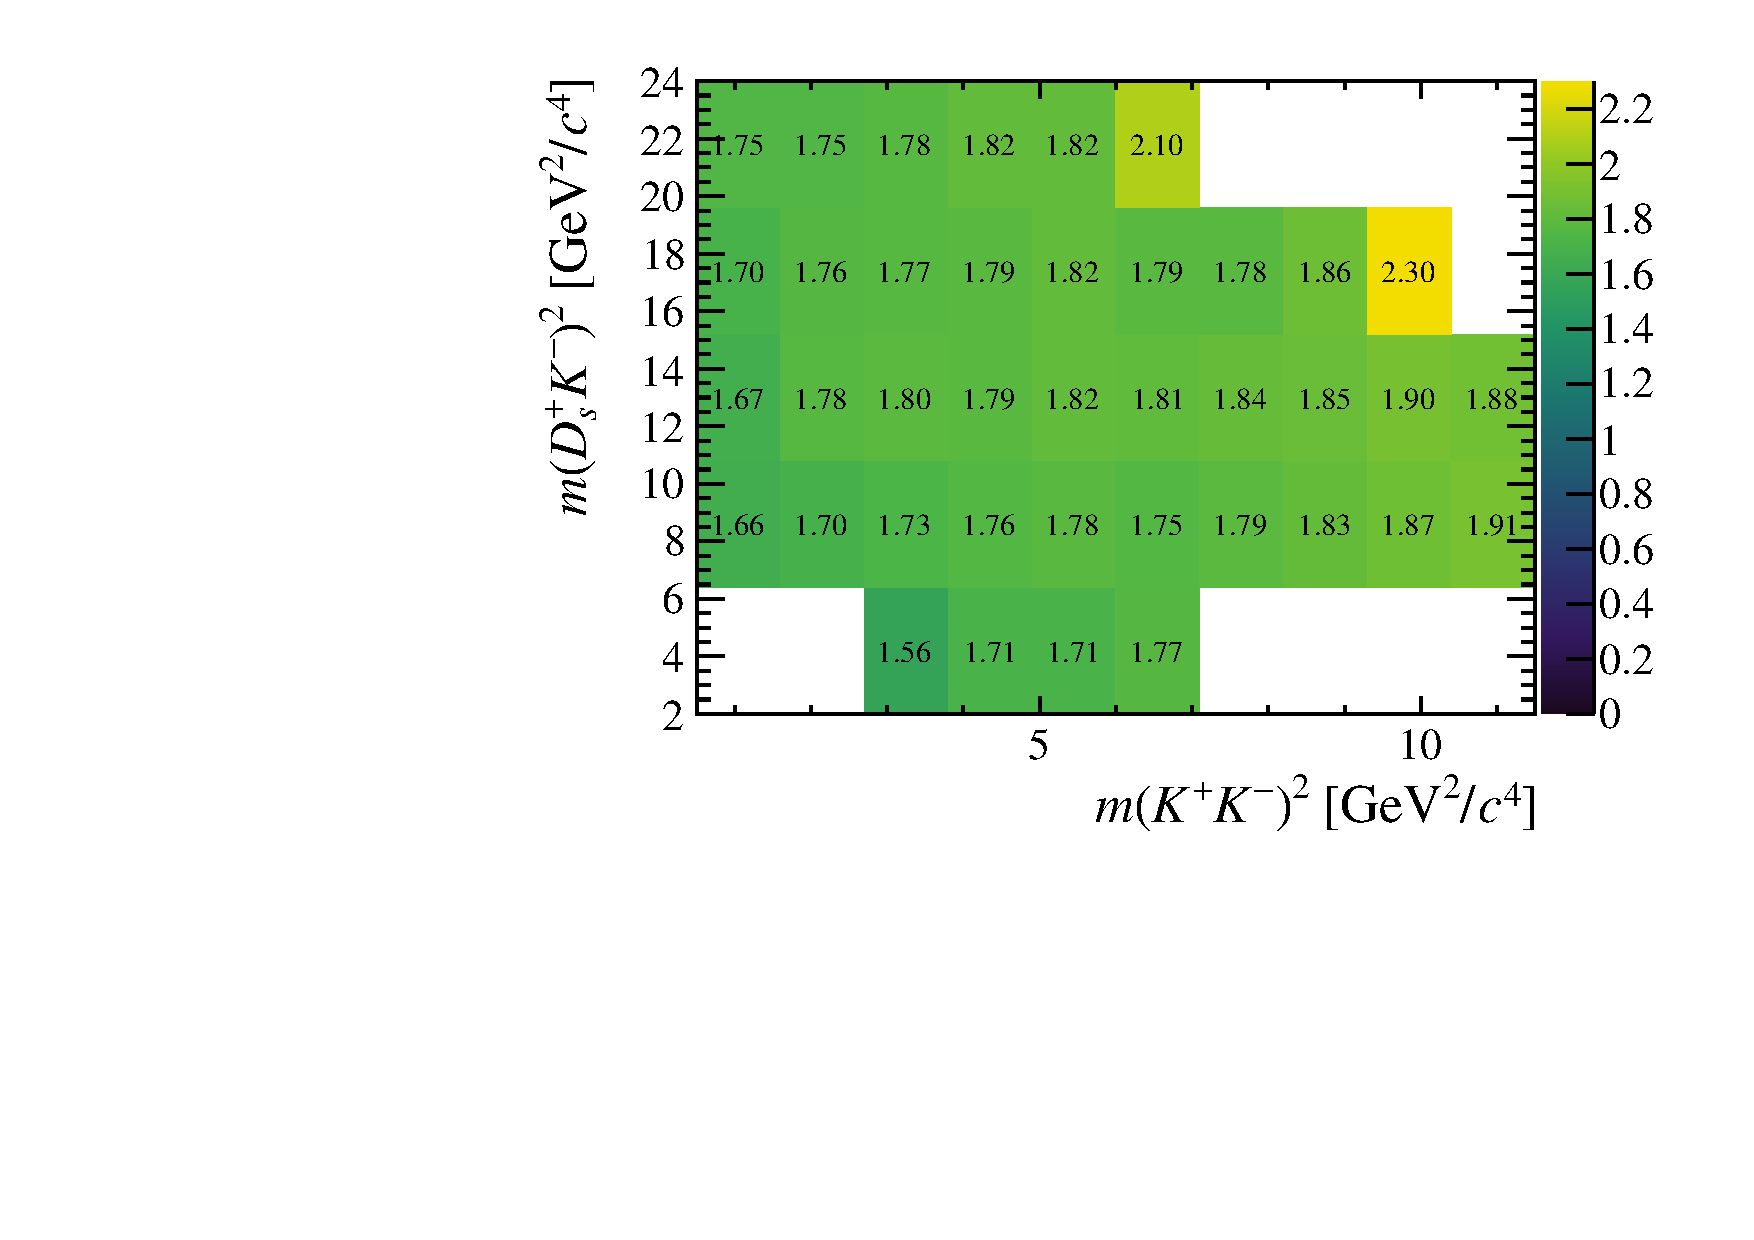
\includegraphics[width=1.0\textwidth]{figs/B2DsKK/Relative_Eff_reco_All.pdf}
        \caption{Reconstruction}
        \label{fig:B2DsKK_releff_reconstruction}
    \end{subfigure}
    \begin{subfigure}[t]{0.40\textwidth}
        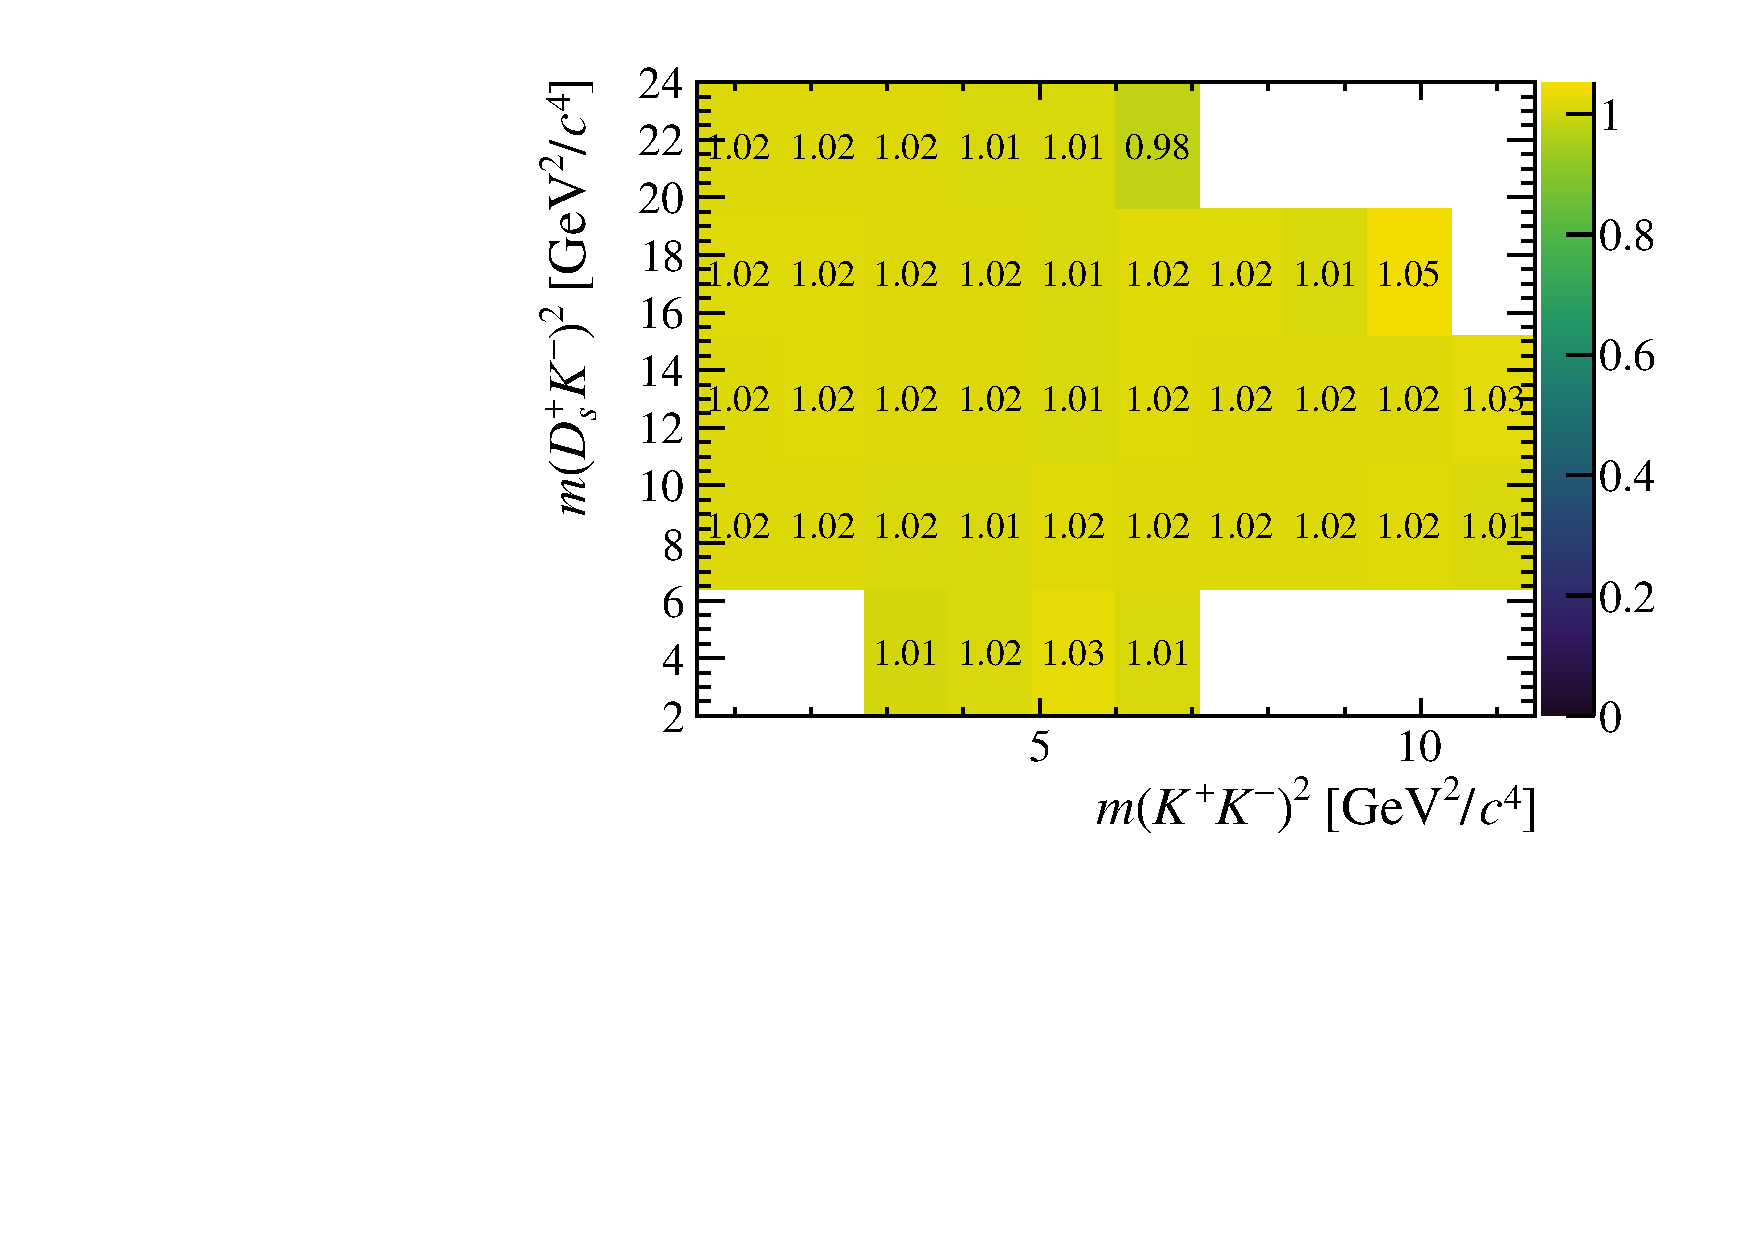
\includegraphics[width=1.0\textwidth]{figs/B2DsKK/Relative_Eff_trig_All.pdf}
        \caption{Trigger}
        \label{fig:B2DsKK_releff_trigger}
    \end{subfigure}
    \begin{subfigure}[t]{0.40\textwidth}
        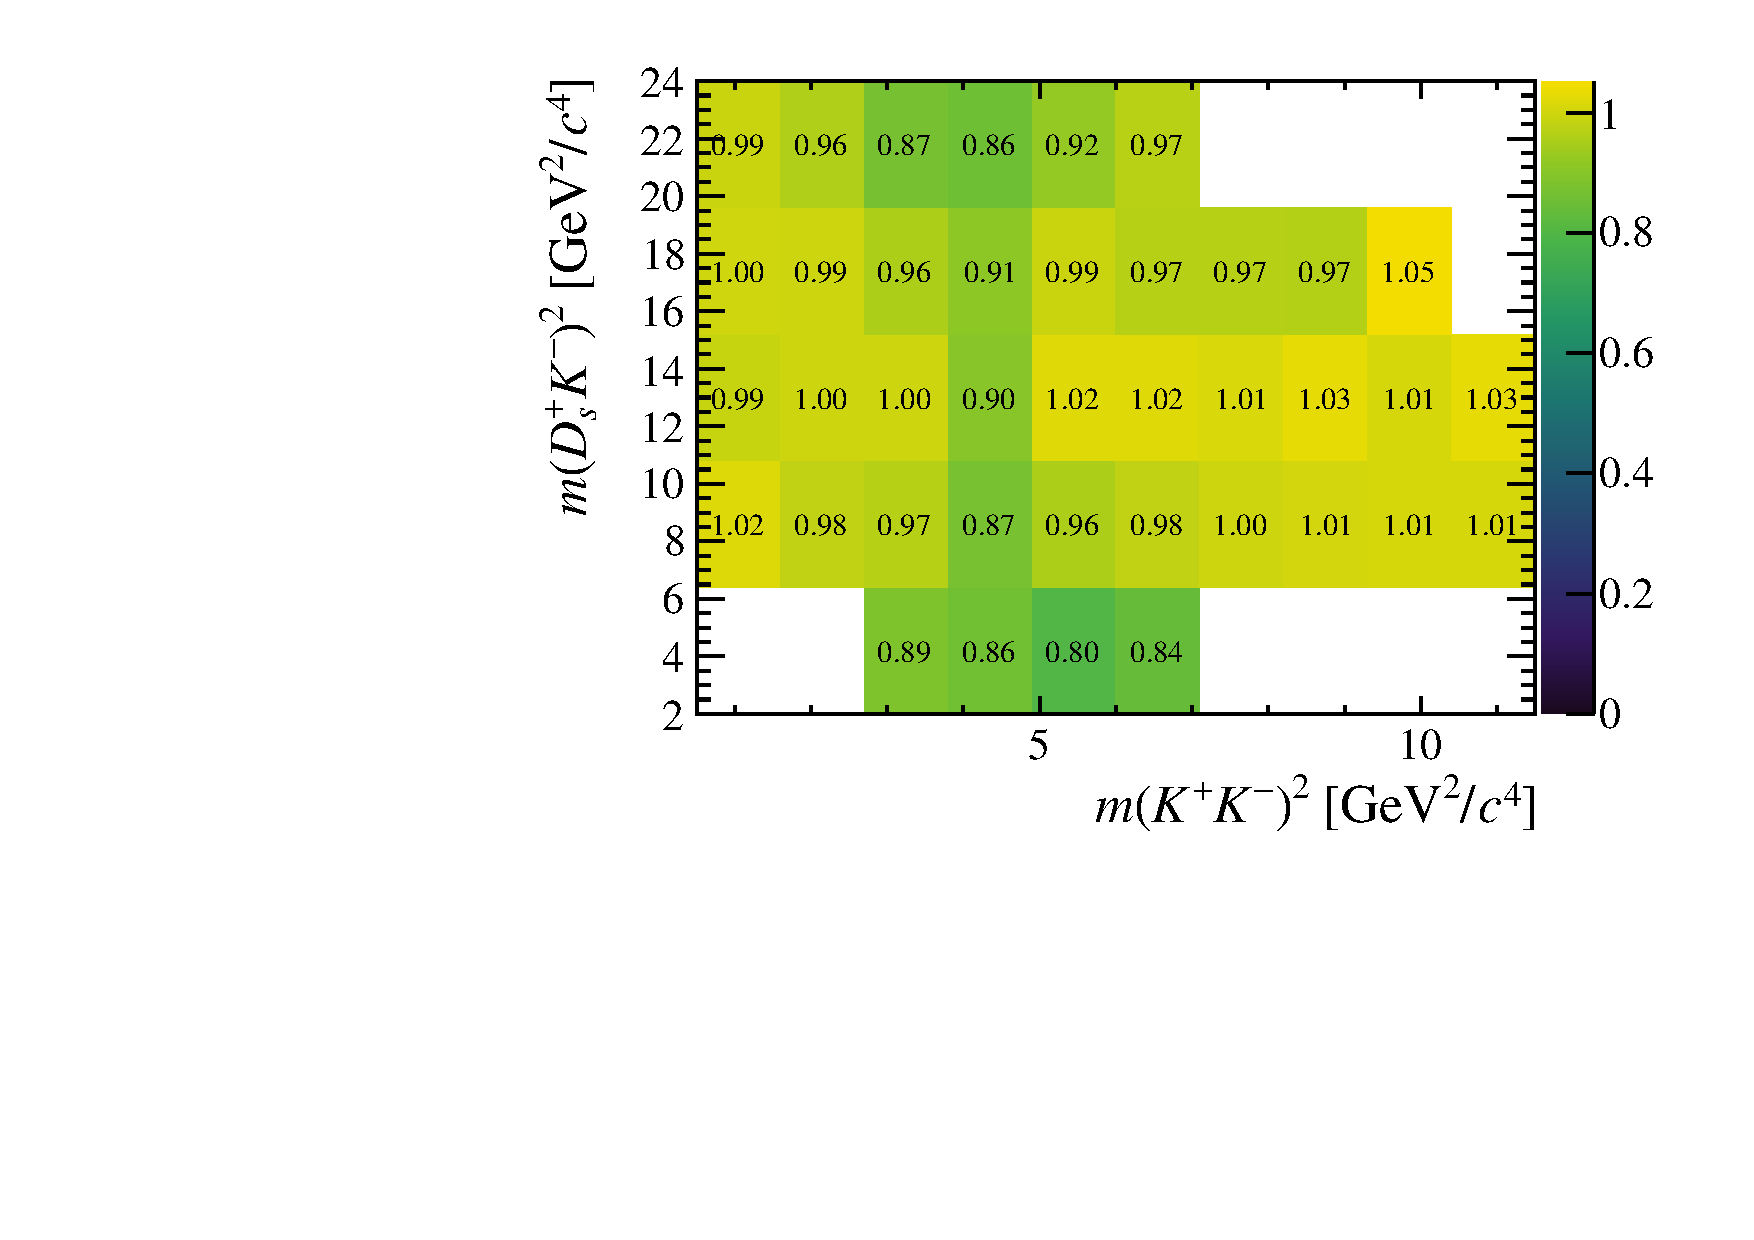
\includegraphics[width=1.0\textwidth]{figs/B2DsKK/Relative_Eff_veto_All.pdf}
        \caption{Vetoes}
        \label{fig:B2DsKK_releff_vetoes}
    \end{subfigure}
    \begin{subfigure}[t]{0.40\textwidth}
        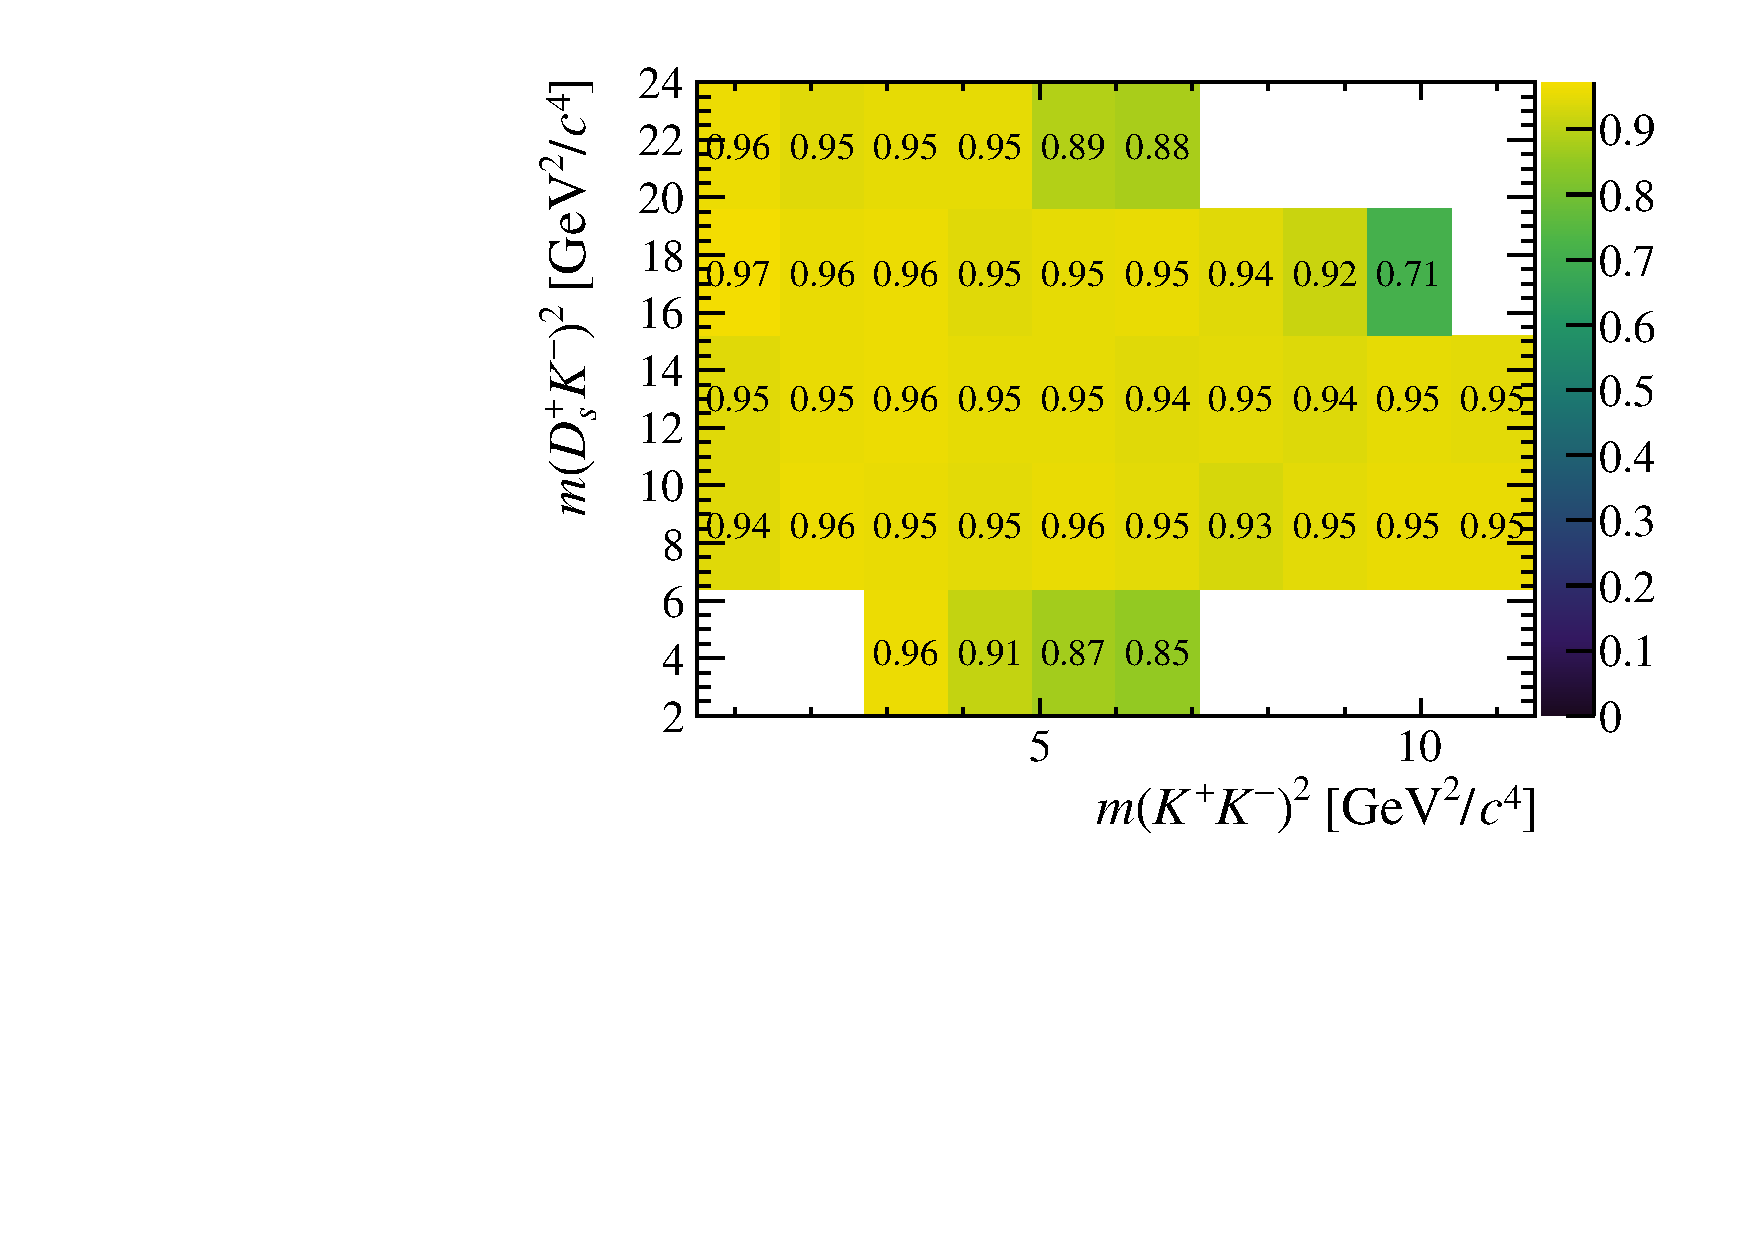
\includegraphics[width=1.0\textwidth]{figs/B2DsKK/Relative_Eff_FDCHI2_All.pdf}
        \caption{Charmless}
        \label{fig:B2DsKK_releff_charmless}
    \end{subfigure}
    \begin{subfigure}[t]{0.40\textwidth}
        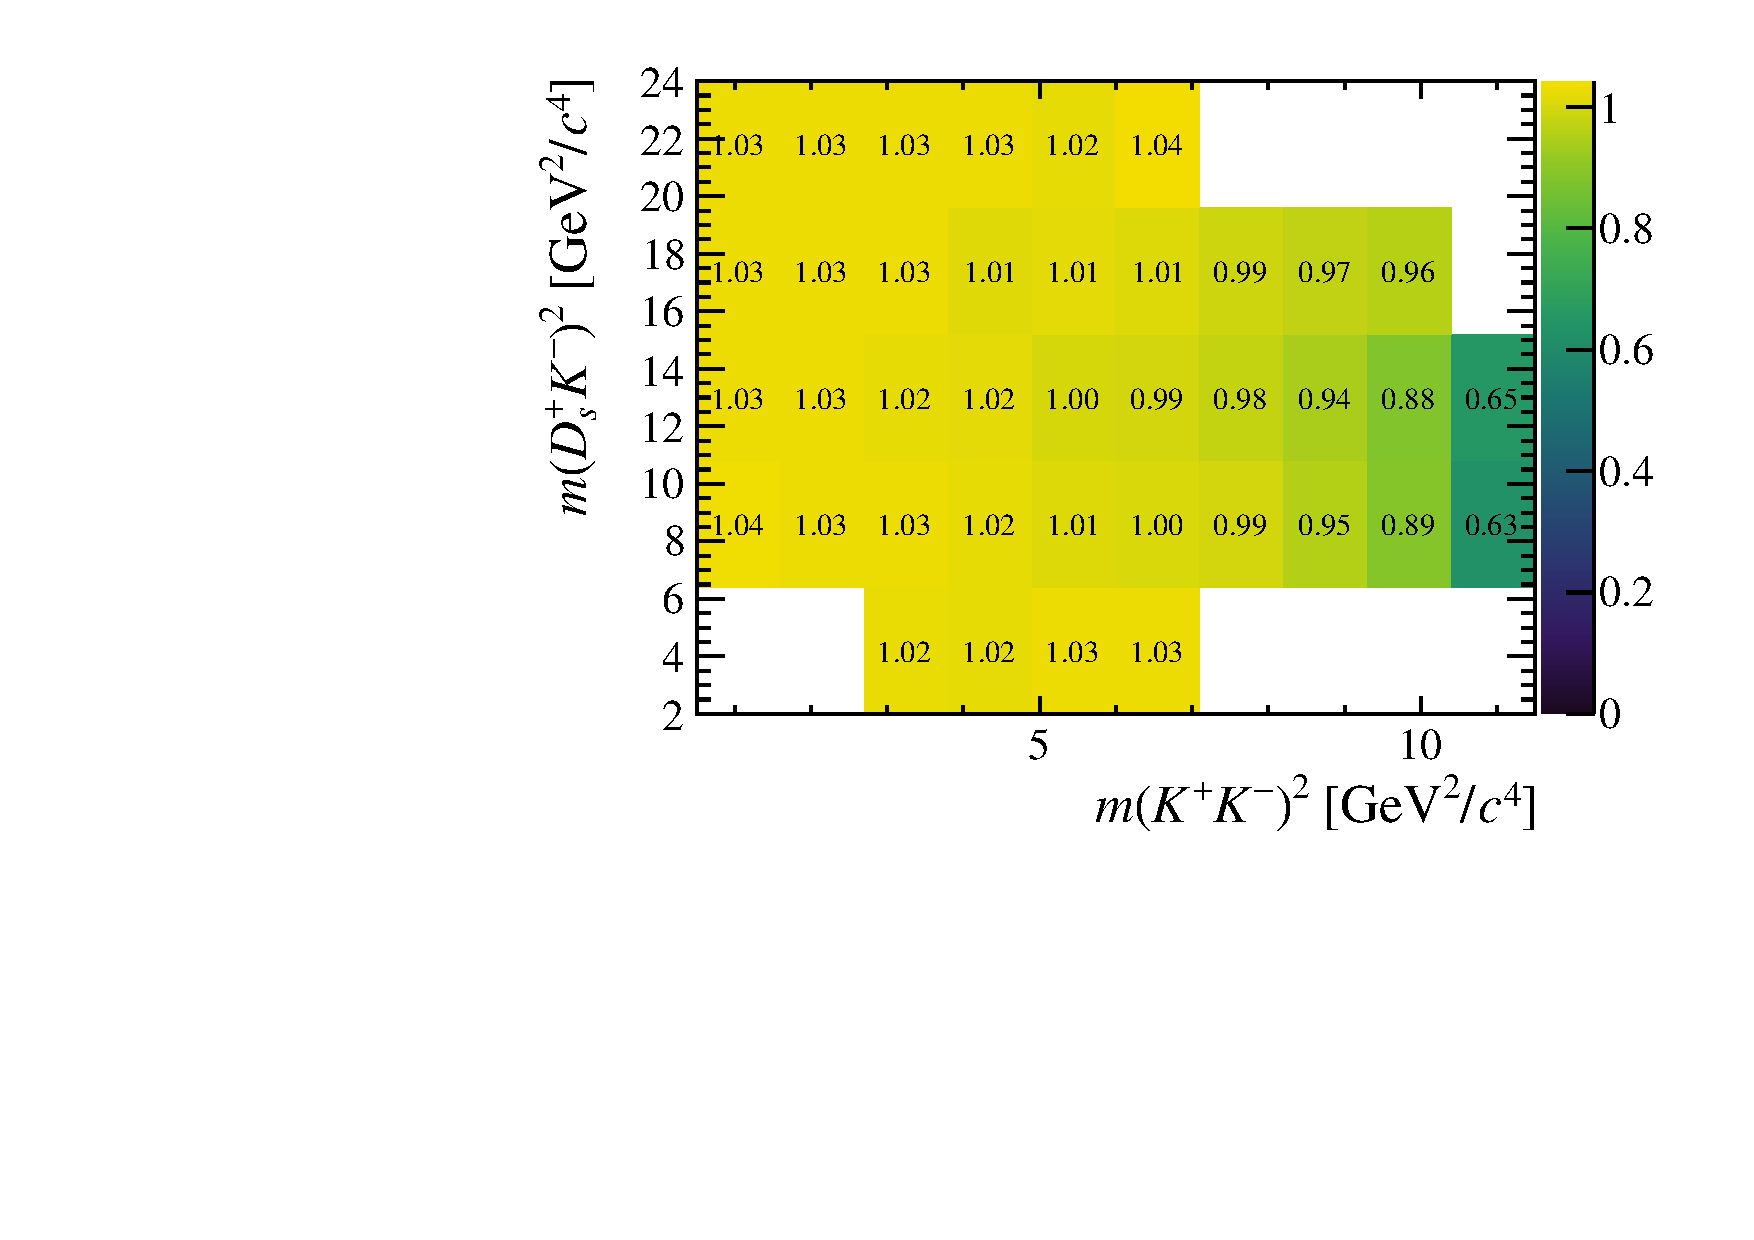
\includegraphics[width=1.0\textwidth]{figs/B2DsKK/Relative_Eff_Bcut_All.pdf}
        \caption{$\chi^{2}_{\text{IP}}$}
        \label{fig:B2DsKK_releff_ipchi2}
    \end{subfigure}
    \begin{subfigure}[t]{0.40\textwidth}
        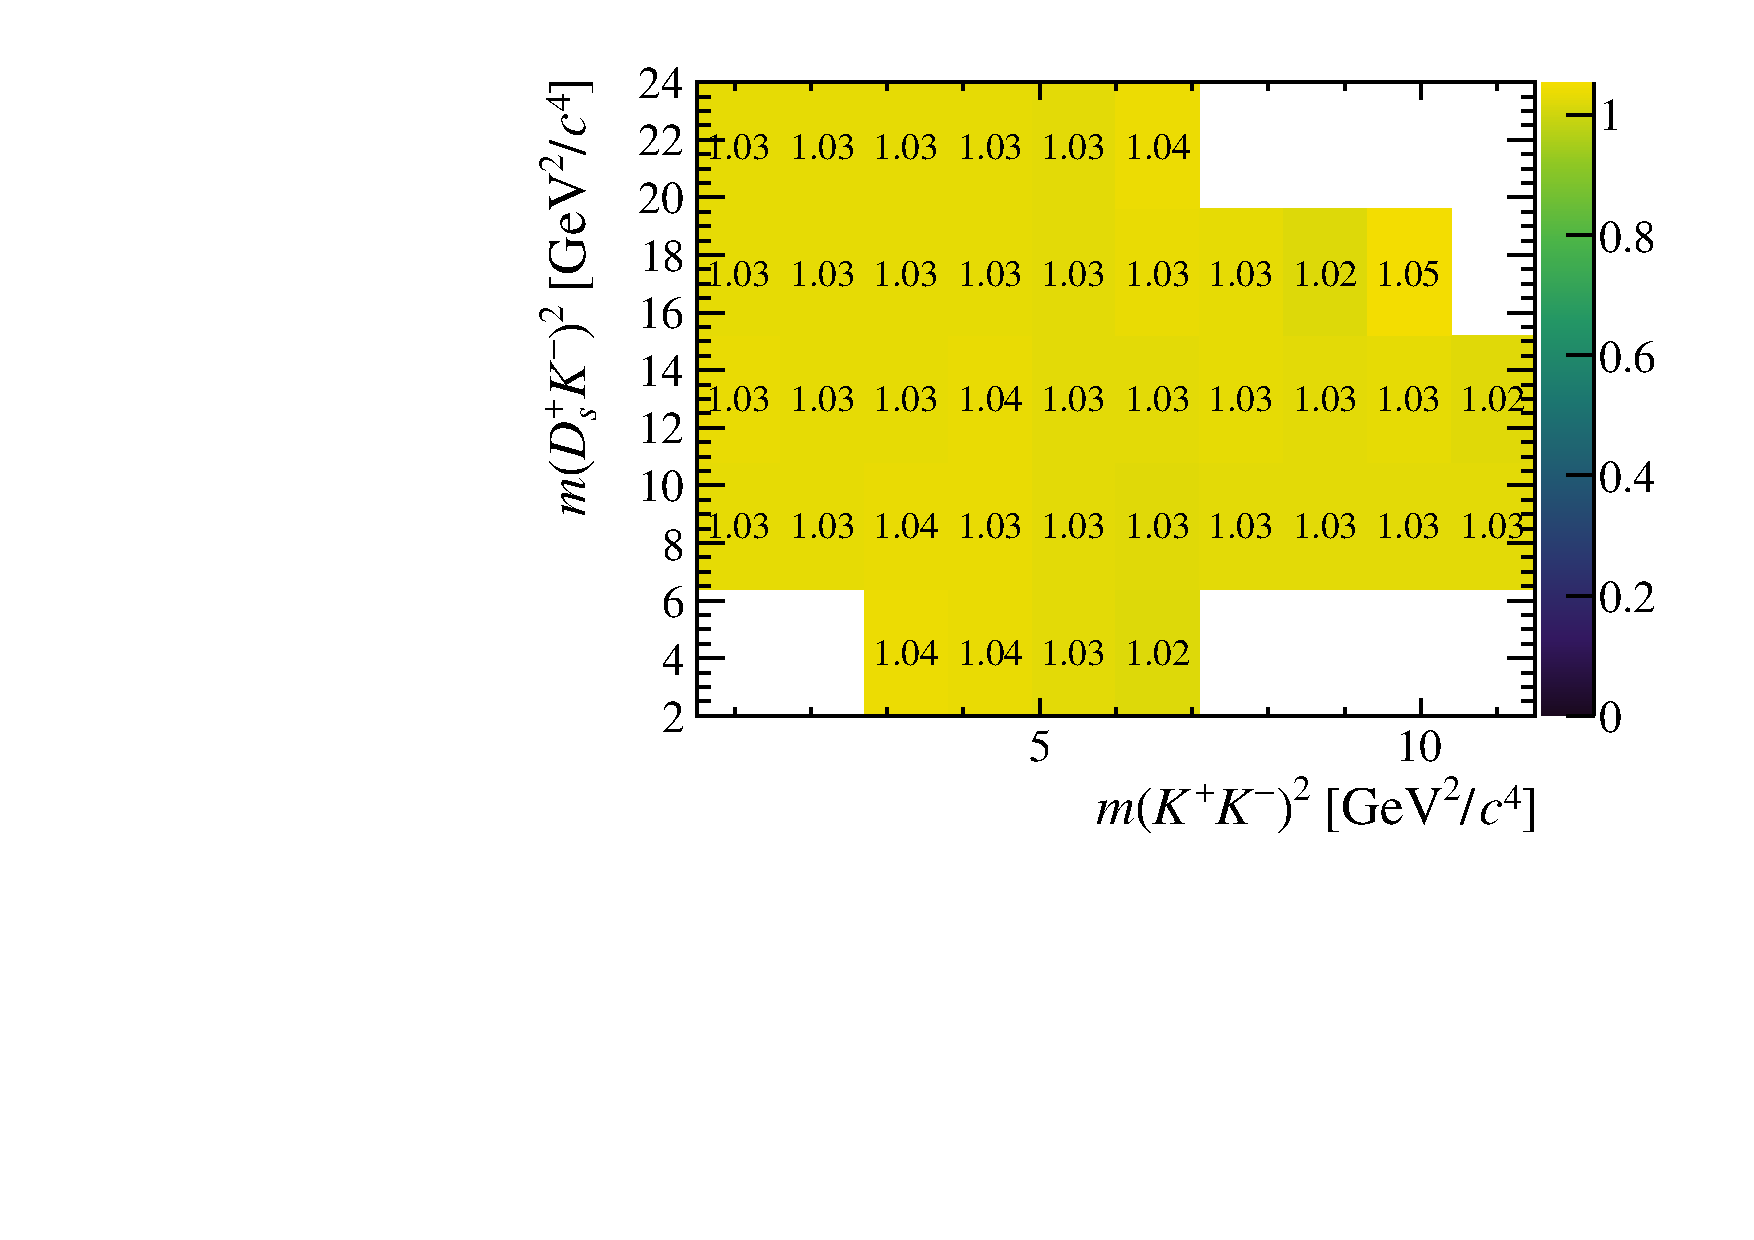
\includegraphics[width=1.0\textwidth]{figs/B2DsKK/Relative_Eff_mass_All.pdf}
        \caption{Mass windows}
        \label{fig:B2DsKK_releff_masswindows}
    \end{subfigure}
    \caption{The relative efficiency $\epsilon_{\text{ratio}}(m^{2}(\Dsp\Km),m^{2}(\Kp\Km))$ as a function of the \decay{\Bp}{\Dsp\Kp\Km} kinematics.}
   \label{fig:B2DsKK_dalitz_eff_one}
\end{figure}
%%%%%%%%%%%%%%%%%%%%%%%%%%%%%%%%%%%%%%%%%%%%%%%%%%%%%%%%%%



% \begin{description}
% \item \textbf{Acceptance:} this accounts for the likelihood for the five final state tracks to be within the \lhcb detector's acceptance. The charged tracks are required to be in the range $10 < \cos\theta < 400 \mrad$, where $\theta$ is the angle between the beam direction and the track. The relative efficiency is shown as a function of the \decay{\Bp}{\Dsp\Kp\Km} Dalitz plot in Fig.\ref{fig:B2DsKK_releff_acceptance}. The relative efficiency is close to one for most of the phase-space. 

% \item \textbf{Reconstruction:} the reconstruction efficiency accounts for the fraction of decays in which all five final state tracks have been correctly reconstructed and pass the \decay{\Bp}{\Dsp\Kp\Km} \emph{Stripping Line} requirements. The reconstruction is only run on events with a positive trigger decision, therefore this also partially accounts for the trigger efficiency. 
% %The \emph{Stripping Line} reconstruction also explicitly requires that at least one trigger has fired for the event to be reconstructed, therefore this efficiency also accounts for part of the trigger efficiency. 
% The distribution of the relative reconstruction efficiency between the signal and normalisation mode is shown in Fig.~\ref{fig:B2DsKK_releff_reconstruction} and is consistently greater than one. In this measurement, the \decay{\Bp}{\Dsp\Dzb} normalisation decays are reconstructed using the same topology as the \decay{\Bp}{\Dsp\Kp\Km} signal. This requires the \Dsp, \Kp and \Km candidates to form a well reconstructed vertex, reducing the efficiency for long-lived \Dzb mesons. 

% %This is greater than one across the whole phase-space as a result of the choice to reconstruct the \decay{\Bp}{\Dsp\Dzb} normalisation decays using the same selection as the \decay{\Bp}{\Dsp\Kp\Km} signal. The latter requires the \Dsp, \Kp and \Km candidates to form a well reconstructed vertex where the \Bp meson decays. However, for the normalisation channel the \Dzb meson travels away from this vertex, so some of the longer lived \Dzb candidates do not pass the vertex quality requirement. This reduces the efficiency for the normalisation channel relative to the signal.

% \end{description}
% % %%%%%%%%%%%%%%%%%%%%%%%%%%%%%%%%%%%%%%%%%%%%%%%%%%%%%%%%%%
% % \begin{figure}[!h]
% %    \centering
% %    \begin{subfigure}[t]{0.45\textwidth}
% %       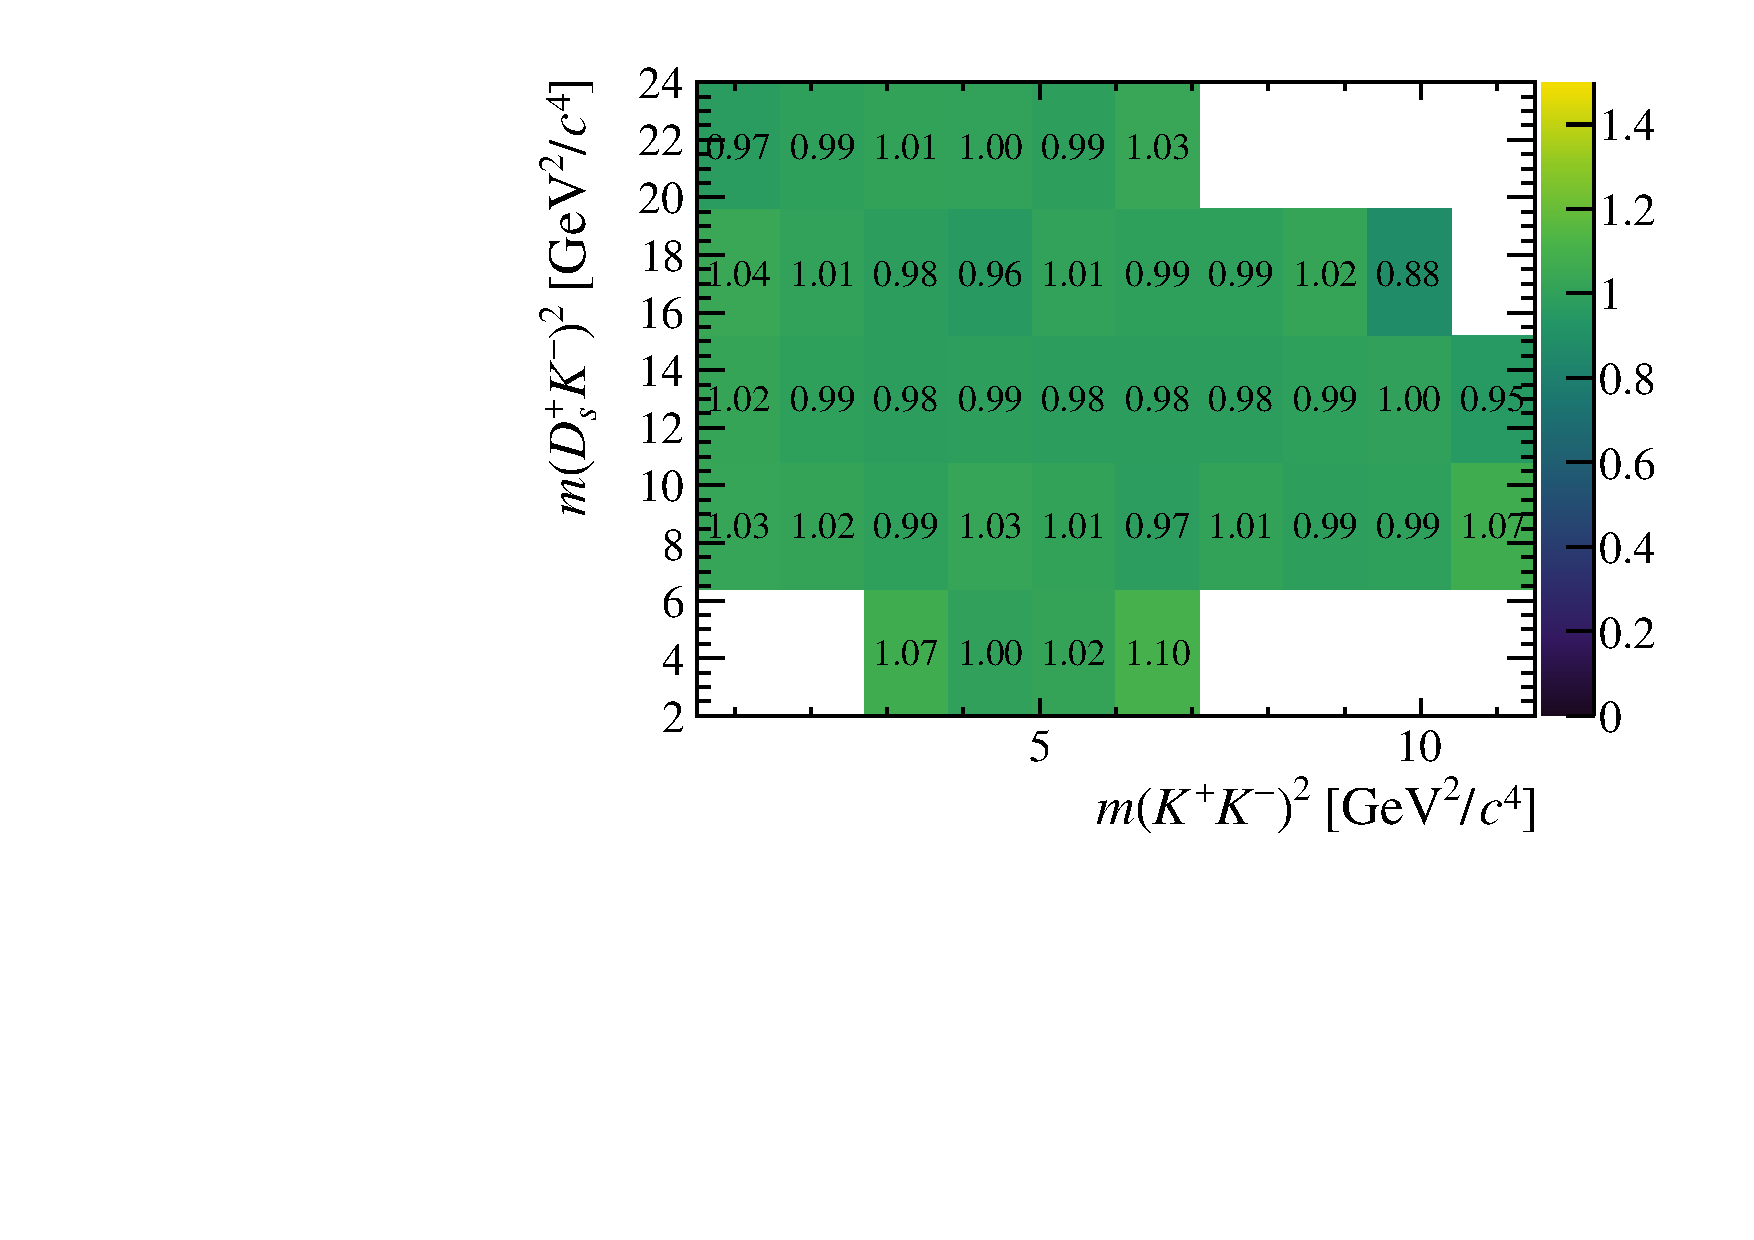
\includegraphics[width=1.0\textwidth]{figs/B2DsKK/Relative_Eff_gen_All_Full.pdf}
% %       \caption{Acceptance}
% %       \label{fig:B2DsKK_releff_acceptance}
% %    \end{subfigure}
% %    \begin{subfigure}[t]{0.45\textwidth}
% %       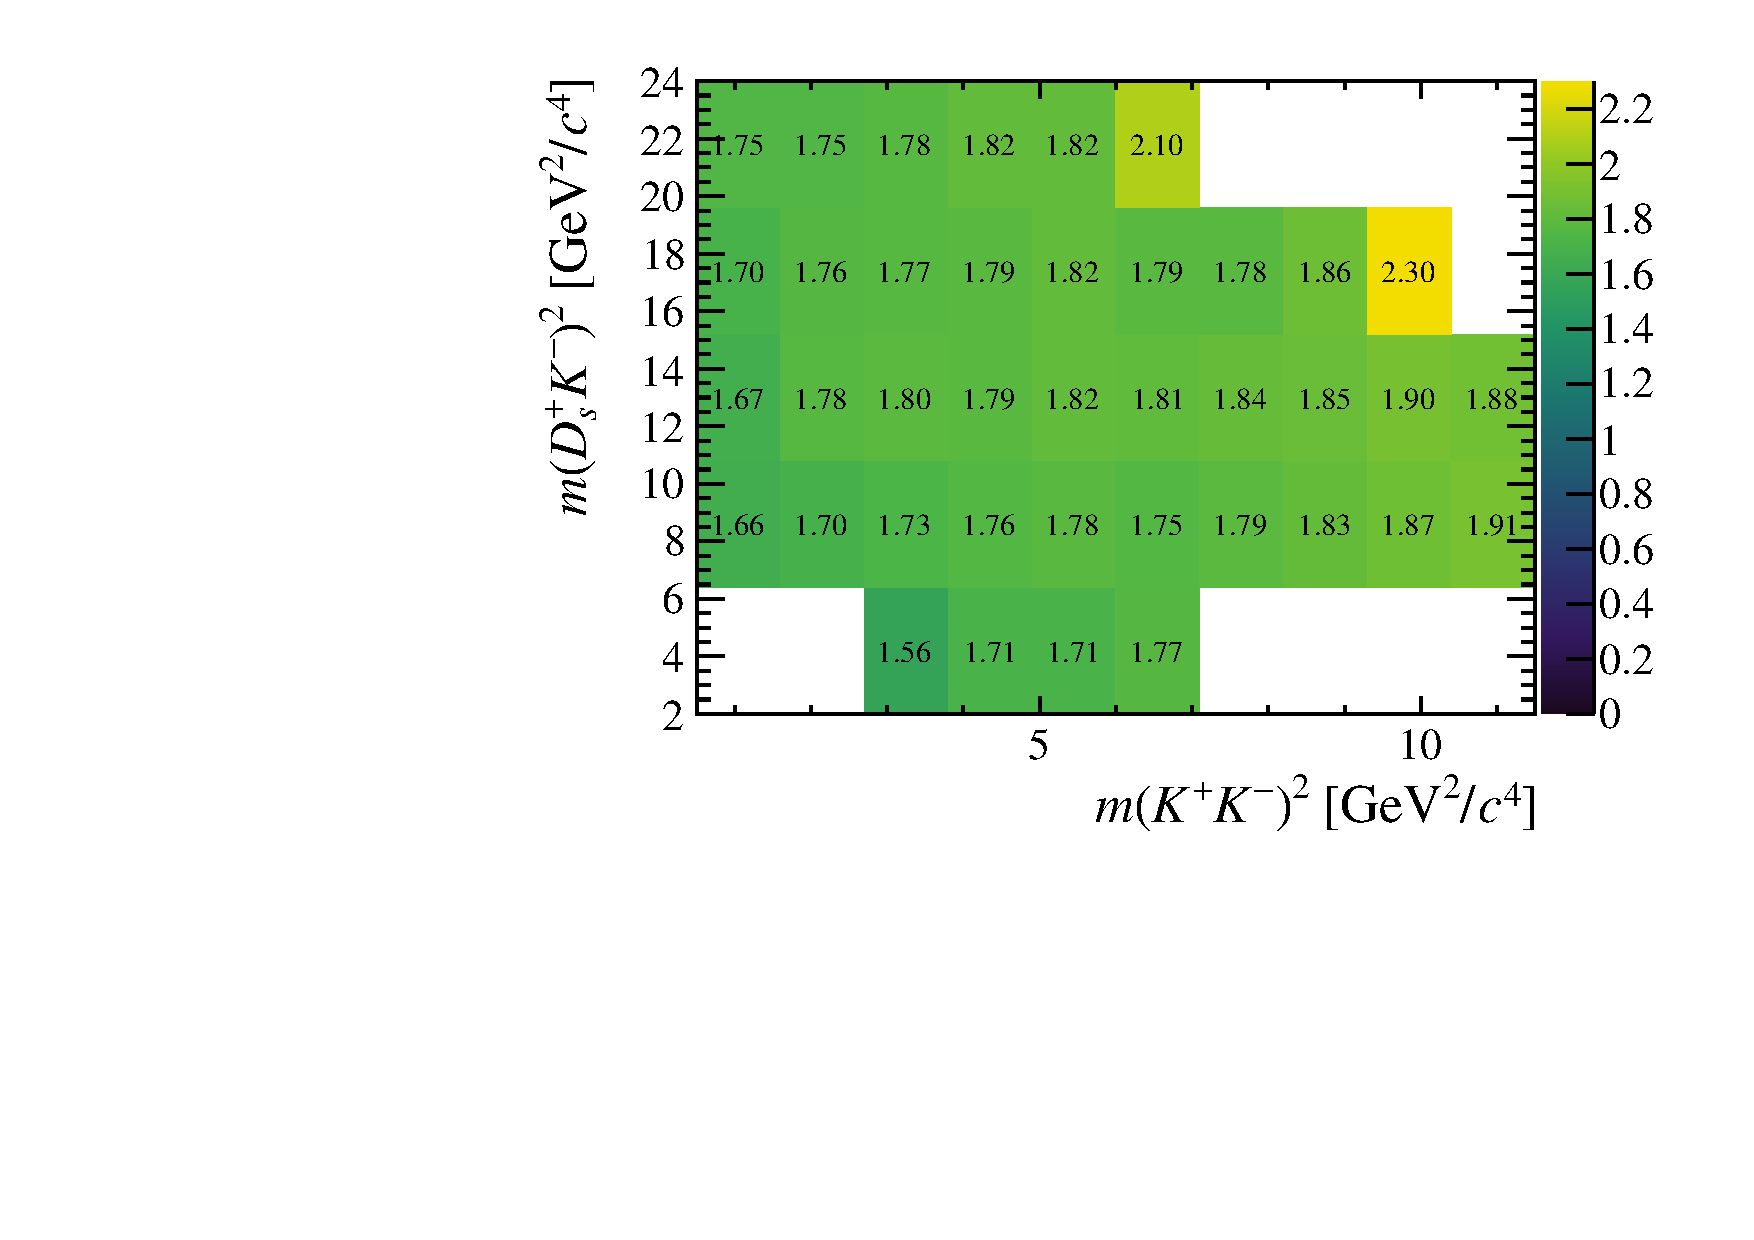
\includegraphics[width=1.0\textwidth]{figs/B2DsKK/Relative_Eff_reco_All.pdf}
% %       \caption{Reconstruction}
% %       \label{fig:B2DsKK_releff_reconstruction}
% %    \end{subfigure}
% %    \caption{The relative efficiency $\epsilon_{\text{ratio}}(m^{2}(\Dsp\Km),m^{2}(\Kp\Km))$ as a function of the \decay{\Bp}{\Dsp\Kp\Km} kinematics.}
% %    \label{fig:B2DsKK_dalitz_eff_one}
% % \end{figure}
% % %%%%%%%%%%%%%%%%%%%%%%%%%%%%%%%%%%%%%%%%%%%%%%%%%%%%%%%%%%


% \begin{description}
% \item \textbf{Trigger:} the trigger efficiency accounts for the fraction of decays for which the signal candidate meets the \texttt{TIS} and \texttt{TOS} requirements outlined in Sec.~\ref{sec:selection_trigger}, given that there was a positive trigger decision in that event. 
% %For the signal and normalisation simulation samples it is very likely that the signal candidate was the cause of the trigger if there was a positive trigger decision, therefore 
% These efficiencies are typically around 95\%. 
% The phase-space distribution of the relative efficiency is very uniform and shown in Fig.~\ref{fig:B2DsKK_releff_trigger}.

% \item \textbf{Vetoes:} this efficiency accounts for the fraction of decays passing the kinematic and normalisation vetoes detailed in Sec.~\ref{sec:kinematicvetos} and \ref{sec:normvetos}. The vetoes to remove misidentified \D and \Lc hadrons are only applied to the \Dsp meson and therefore assumed to affect the signal and normalisation mode equally. The systematic uncertainty arising from this choice is discussed in Sections~\ref{sec:B2DsKK_sys_releff}. 
% The veto to remove the normalisation channel \decay{\Bp}{\Dsp(\decay{\Dzb}{\Kp\Km})} is not included in this figure as the mass window is narrower than the bin width, and would bias the efficiency for other candidates within the same bin. The area of phase-space excluded by the veto will not be sampled in the final result.
% %Although the veto for misidentified normalisation decays proceeding via \decay{\Dzb}{\Kp\pim} decays is included, the veto to remove correctly reconstructed normalisation decays with \decay{\Dzb}{\Kp\Km} is not included. This is because the width of this veto is less that the binning width so it would therefore lead to the wrong efficiency for candidates within in the same bin but not in the window. This doesn't affect the final result, it simply means areas of the efficiency Dalitz plot are populated that will never be sampled. 
% The distribution of the relative efficiency is shown in Fig.~\ref{fig:B2DsKK_releff_vetoes}. 
% A vertical band is clear in the centre as a result of the veto for misidentified normalisation decays with \decay{\Dzb}{\Kp\pim}.
% \end{description}

% % %%%%%%%%%%%%%%%%%%%%%%%%%%%%%%%%%%%%%%%%%%%%%%%%%%%%%%%%%%
% % \begin{figure}[!h]
% %    \centering
% %    \begin{subfigure}[t]{0.45\textwidth}
% %       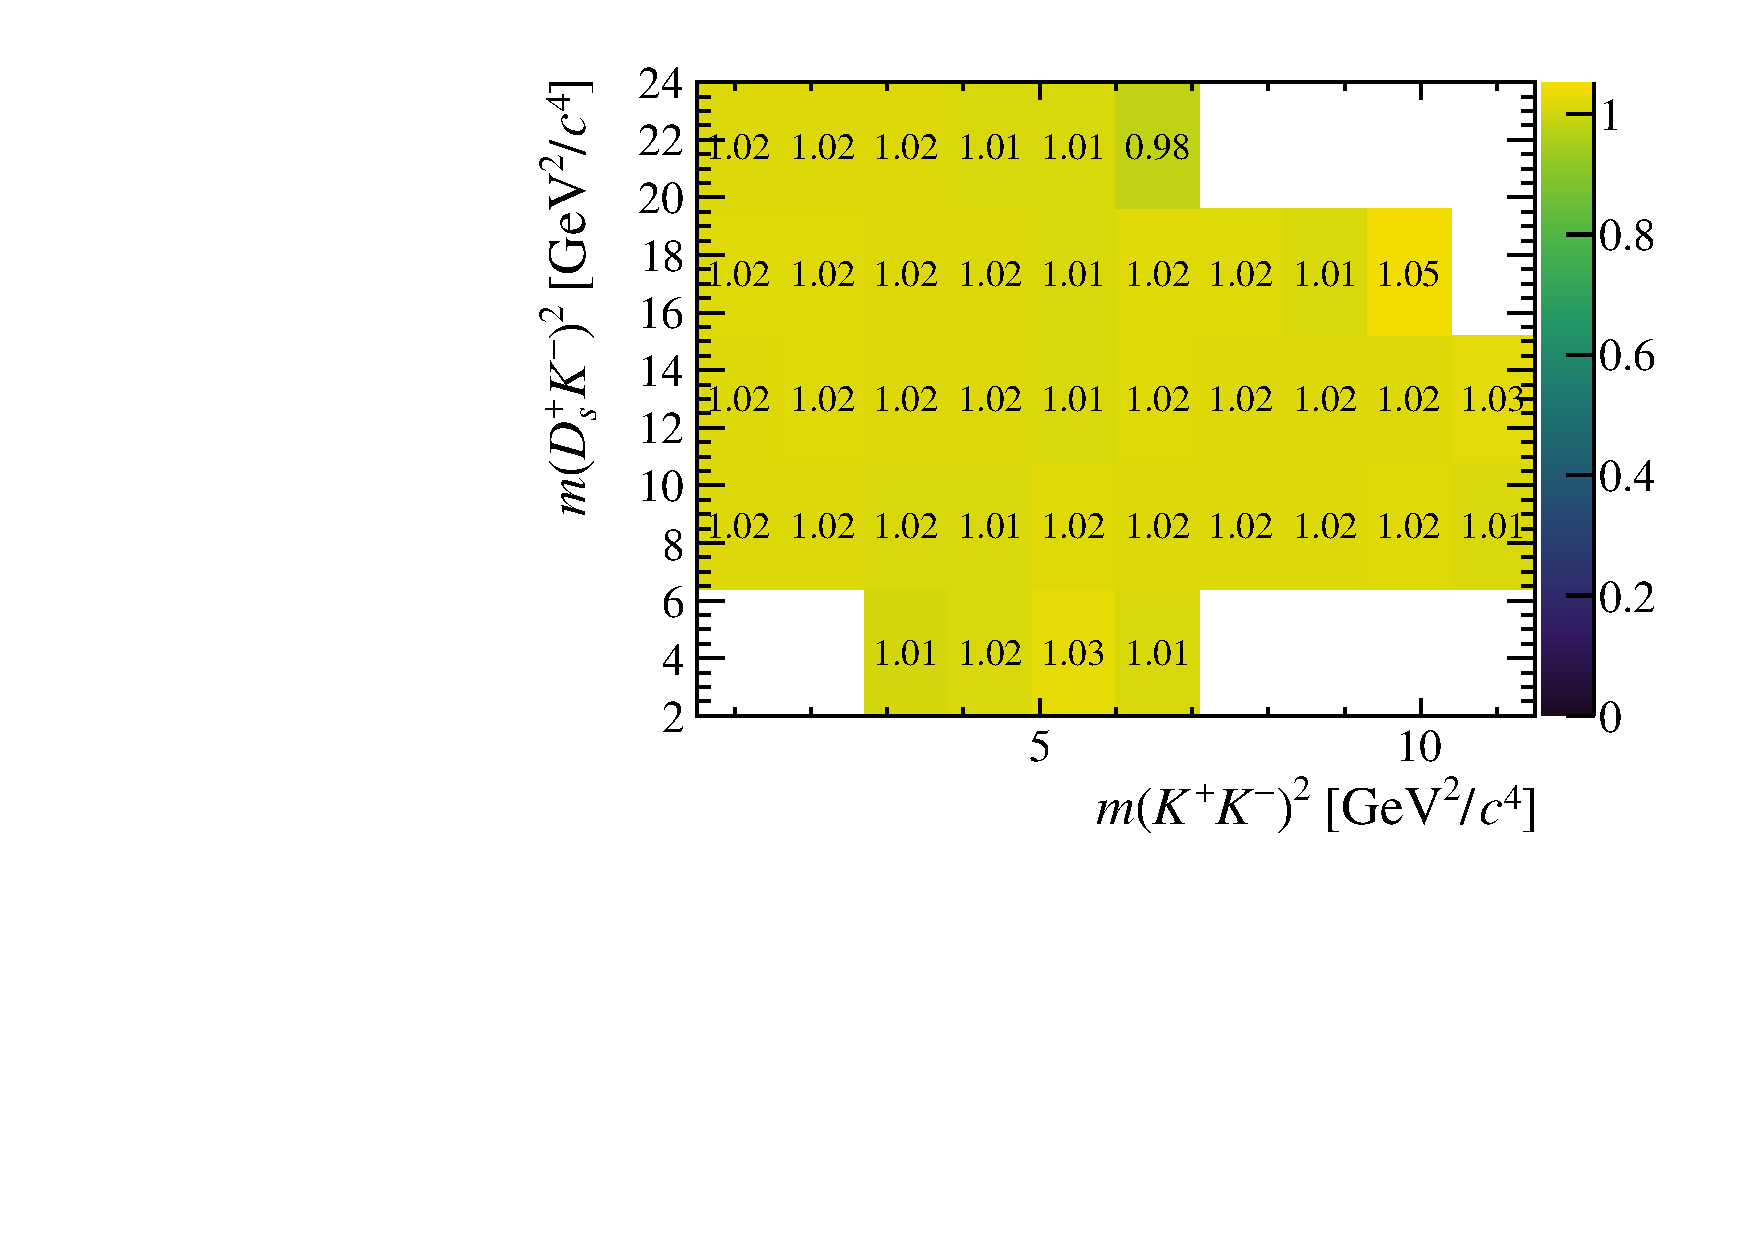
\includegraphics[width=1.0\textwidth]{figs/B2DsKK/Relative_Eff_trig_All.pdf}
% %       \caption{Trigger}
% %       \label{fig:B2DsKK_releff_trigger}
% %    \end{subfigure}
% %    \begin{subfigure}[t]{0.45\textwidth}
% %       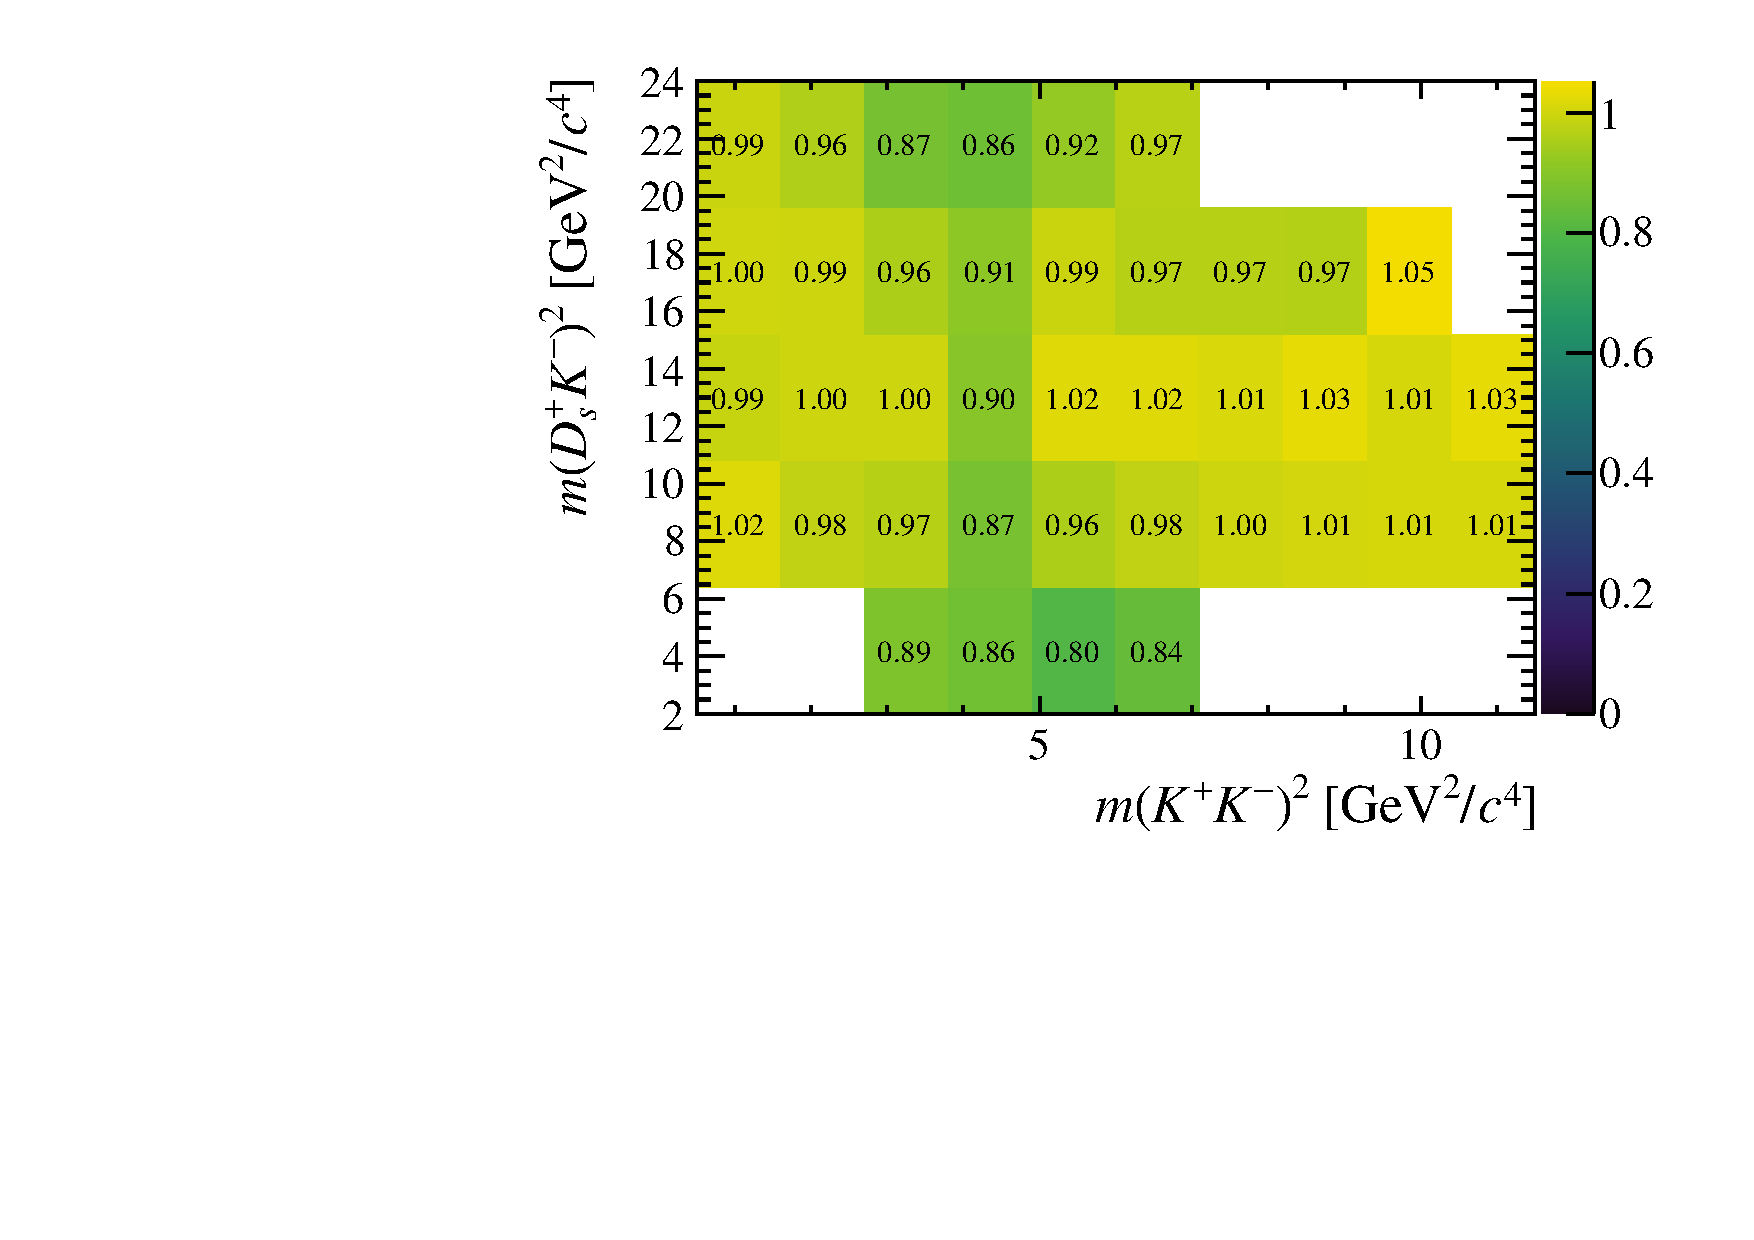
\includegraphics[width=1.0\textwidth]{figs/B2DsKK/Relative_Eff_veto_All.pdf}
% %       \caption{Vetoes}
% %       \label{fig:B2DsKK_releff_vetoes}
% %    \end{subfigure}
% %    \caption{The relative efficiency $\epsilon_{\text{ratio}}(m^{2}(\Dsp\Km),m^{2}(\Kp\Km))$ as a function of the \decay{\Bp}{\Dsp\Kp\Km} kinematics.}
% %    \label{fig:B2DsKK_dalitz_eff_one}
% % \end{figure}
% % %%%%%%%%%%%%%%%%%%%%%%%%%%%%%%%%%%%%%%%%%%%%%%%%%%%%%%%%%%

% \begin{description}

% \item \textbf{Charmless:} this accounts for the fraction of decays failing the requirements on the \D meson flight distance requirements aimed at removing charmless and single-charm backgrounds. The distribution shown in Fig.\ref{fig:B2DsKK_releff_charmless} shows a fairly flat distribution with the exception of some of the edge bins.
% \item \textbf{$\chi^{2}_{\text{IP}}$:} this accounts for the fraction of decays that pass the requirements on the \Bp and \Dsp meson impact parameter significance. The relative efficiency is shown in Fig.~\ref{fig:B2DsKK_releff_ipchi2} and shows a strong dependency on phase-space at high $m^{2}(\Kp\Km)$. The lower relative efficiencies at high $m^{2}(\Kp\Km)$ may be because the \Dsp mesons are produced collinear with the \Bp direction and may fail the minimum impact parameter significance requirement.
% \end{description}

% % %%%%%%%%%%%%%%%%%%%%%%%%%%%%%%%%%%%%%%%%%%%%%%%%%%%%%%%%%%
% % \begin{figure}[!h]
% %    \centering
% %    \begin{subfigure}[t]{0.45\textwidth}
% %       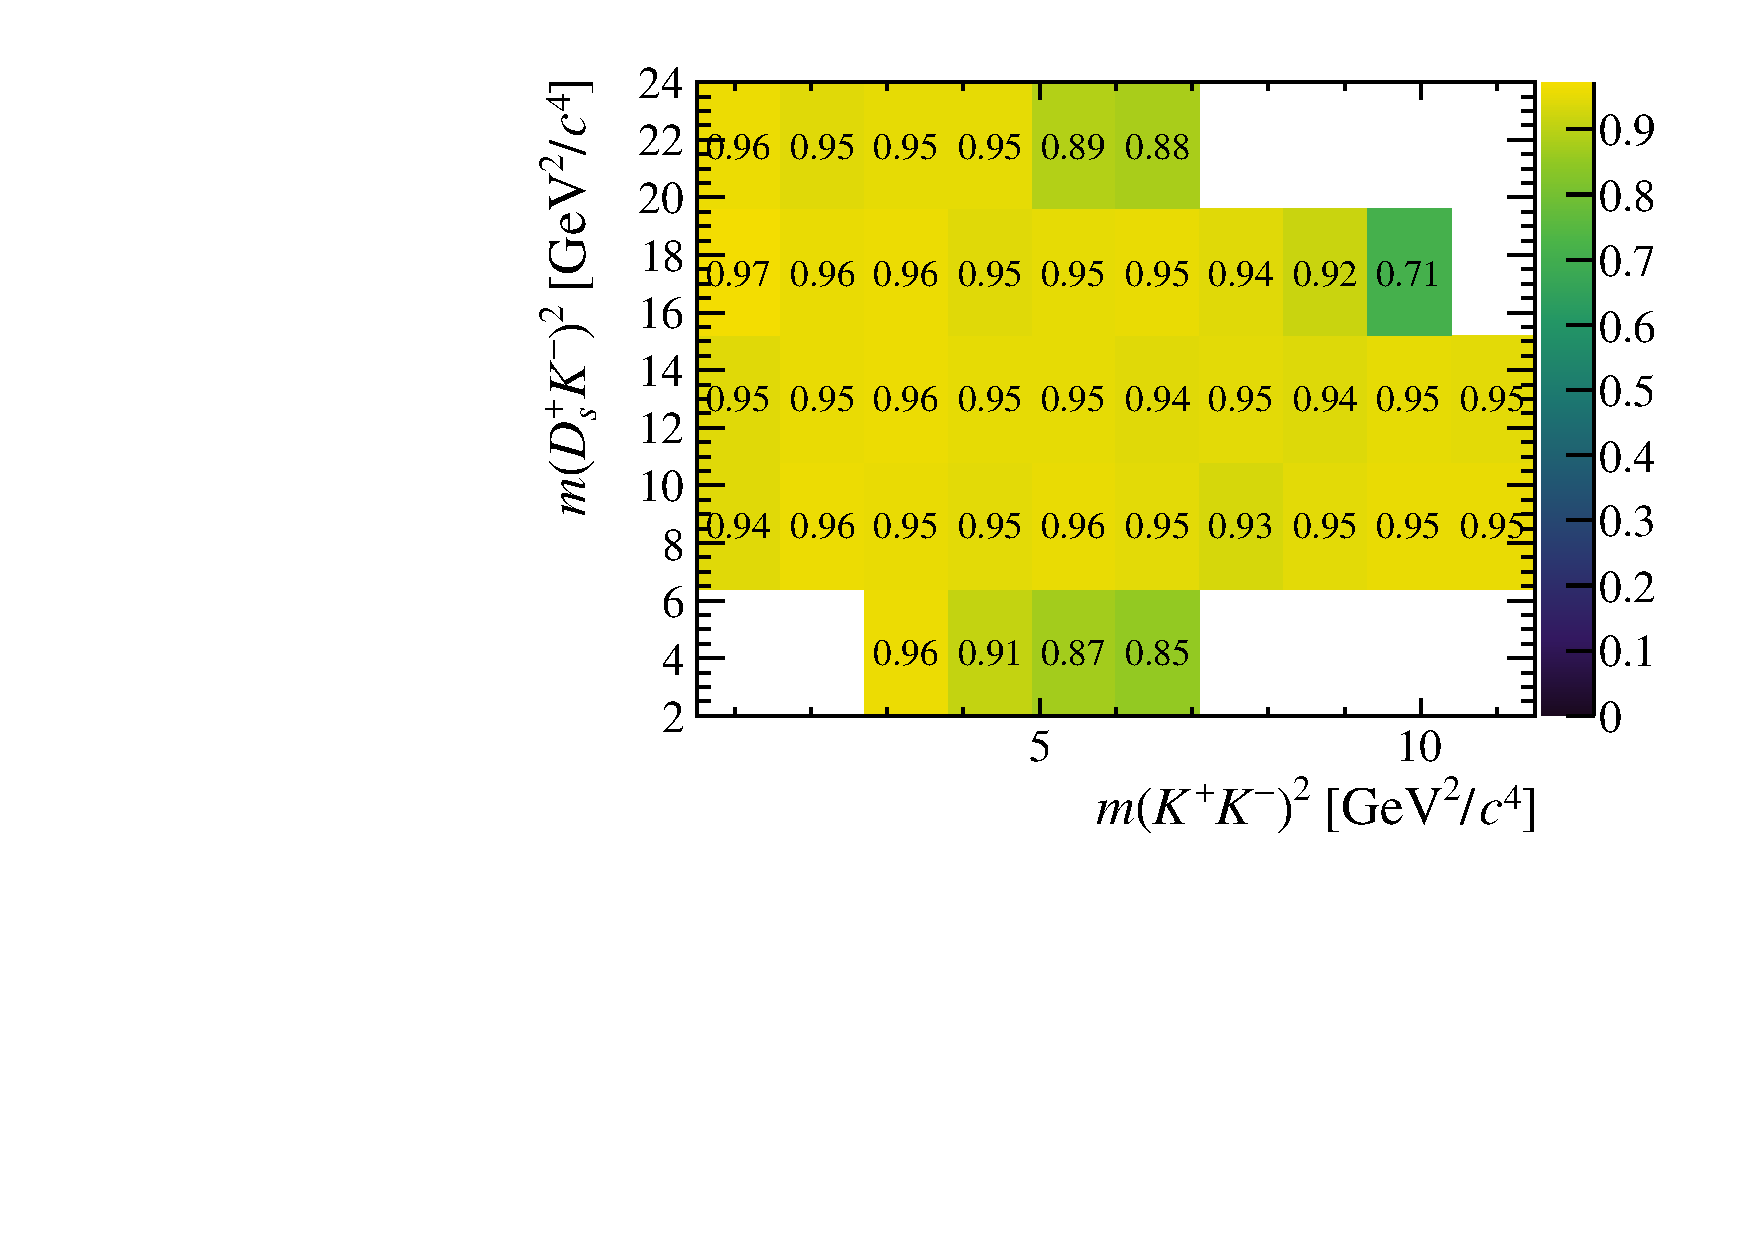
\includegraphics[width=1.0\textwidth]{figs/B2DsKK/Relative_Eff_FDCHI2_All.pdf}
% %       \caption{Charmless}
% %       \label{fig:B2DsKK_releff_charmless}
% %    \end{subfigure}
% %    \begin{subfigure}[t]{0.45\textwidth}
% %       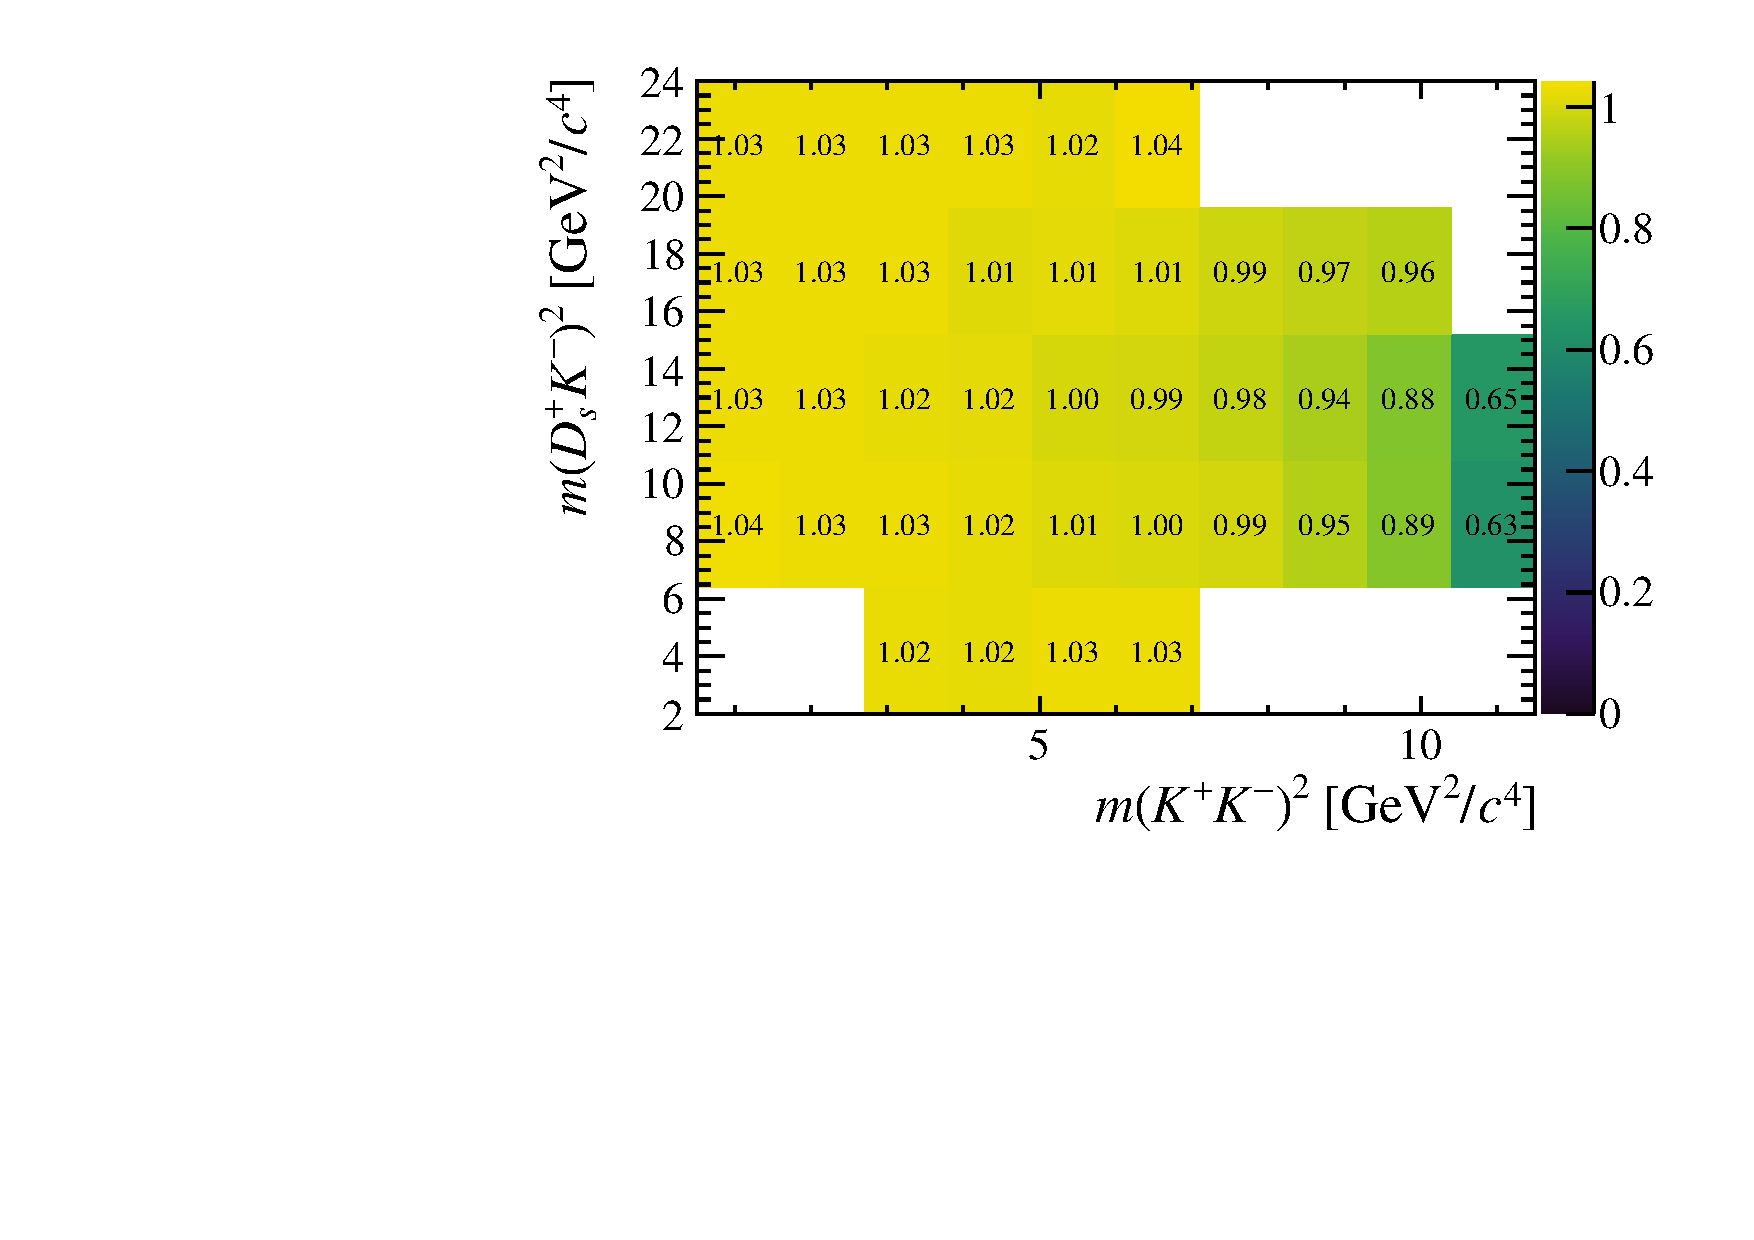
\includegraphics[width=1.0\textwidth]{figs/B2DsKK/Relative_Eff_Bcut_All.pdf}
% %       \caption{$\chi^{2}_{\text{IP}}$}
% %       \label{fig:B2DsKK_releff_ipchi2}
% %    \end{subfigure}
% %    \caption{The relative efficiency $\epsilon_{\text{ratio}}(m^{2}(\Dsp\Km),m^{2}(\Kp\Km))$ as a function of the \decay{\Bp}{\Dsp\Kp\Km} kinematics.}
% %    \label{fig:B2DsKK_dalitz_eff_two}
% % \end{figure}
% % %%%%%%%%%%%%%%%%%%%%%%%%%%%%%%%%%%%%%%%%%%%%%%%%%%%%%%%%%%

% \begin{description}
% \item \textbf{Mass windows:} this accounts for the fraction of decays that pass the mass windows around the \Dsp and \Dzb masses. No requirement is placed on the \Kp\Km pair, therefore the relative efficiency shown in Fig.~\ref{fig:B2DsKK_releff_masswindows} is slightly greater than one across the whole phase-space. 
% \end{description}



% % %%%%%%%%%%%%%%%%%%%%%%%%%%%%%%%%%%%%%%%%%%%%%%%%%%%%%%%%%%
% % \begin{figure}[!h]
% %    \centering
% %    \begin{subfigure}[t]{0.45\textwidth}
% %       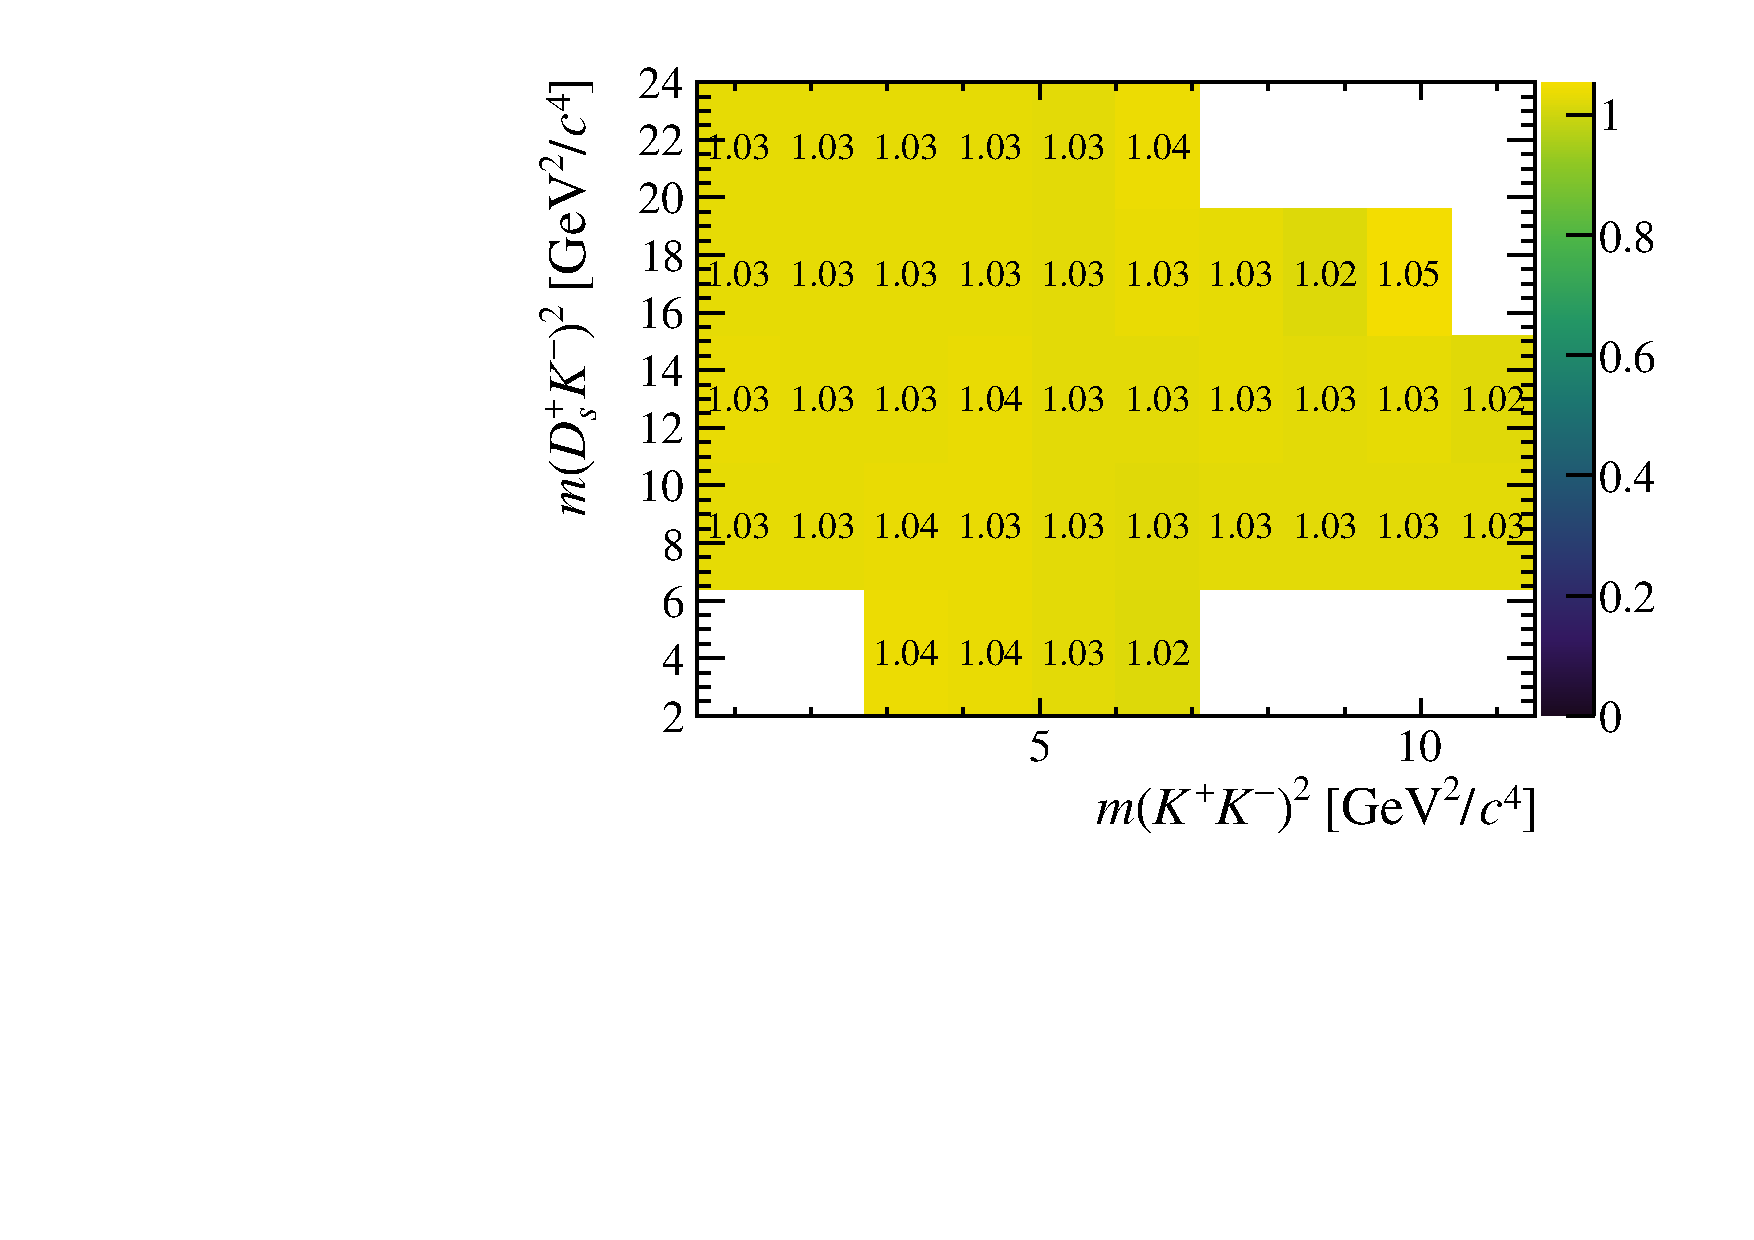
\includegraphics[width=1.0\textwidth]{figs/B2DsKK/Relative_Eff_mass_All.pdf}
% %       \caption{Mass windows}
% %       \label{fig:B2DsKK_releff_masswindows}
% %    \end{subfigure}
% %    \caption{The relative efficiency $\epsilon_{\text{ratio}}(m^{2}(\Dsp\Km),m^{2}(\Kp\Km))$ as a function of the \decay{\Bp}{\Dsp\Kp\Km} kinematics.}
% %    \label{fig:B2DsKK_dalitz_eff_two}
% % \end{figure}
% % %%%%%%%%%%%%%%%%%%%%%%%%%%%%%%%%%%%%%%%%%%%%%%%%%%%%%%%%%%


\subsection{Efficiencies requiring calibration samples} 
\label{sec:B2DsKK_eff_from_calib}

\subsubsection{PID efficiency}
The relative PID efficiency shown in Fig.~\ref{fig:B2DsKK_releff_PID} are calculated by correcting the PID variables in simulation using a package called \pidcalib~\cite{PIDCalib}. 
%This uses calibrations samples for the different particle species to determine the distribution of the PID variables in data. 
A calibration sample of \decay{\Dstarp}{(\decay{\Dz}{\Kp\pim})\pip} decays is background-subtracted to isolate the distributions of the PID variables for the \Kp and \pim tracks. 
%The calibration samples for both \Kp and \pip mesons are collected from samples of \decay{\Dstarp}{(\decay{\Dz}{\Kp\pim})\pip} decays, using the decay products of the \Dz decay. 
%Additionally, samples of protons are collected from \decay{\PLambda}{\proton\pim} decays. 
The PID variable distributions depend on both the kinematics of the track and the occupancy of the detector. 
%These can both affect the characteristics of the hits in the \rich sub-detectors and therefore result in different PID variable distributions. 
The calibrations samples are characterised using three variables; the transverse momentum of the track \pt, the pseudo-rapidity \Peta, and the number of tracks in an event $n_{\text{Tracks}}$. 
The calibration PID variables are parametrised using an unbinned approach that creates four dimensional PDFs (PID,\Peta,\pt,$n_{\text{Tracks}}$) from the calibration samples using a kernel density estimation implemented with the \meerkat package~\cite{Meerkat}. 
Similar four dimensional PDFs are created for simulation samples of the calibration modes. These two PDFs are used to calculate the transformation needed for each species as a function of (PID,\Peta,\pt,$n_{\text{Tracks}}$) to correct the distribution in simulation. 
This transformation preserves the correlations between the different PID variables and between the PID and kinematic properties. 
%This correction is applied to both the DLL PID variables and ProbNNx variables used in the MVA selection. 
%The phase-space distribution of the relative PID efficiency between the signal and normalisation channel is shown in Fig.~\ref{fig:B2DsKK_releff_PID}.

%%%%%%%%%%%%%%%%%%%%%%%%%%%%%%%%%%%%%%%%%%%%%%%%%%%%%%%%%%
\begin{figure}[!h]
   \centering
   \begin{subfigure}[t]{0.4\textwidth}
      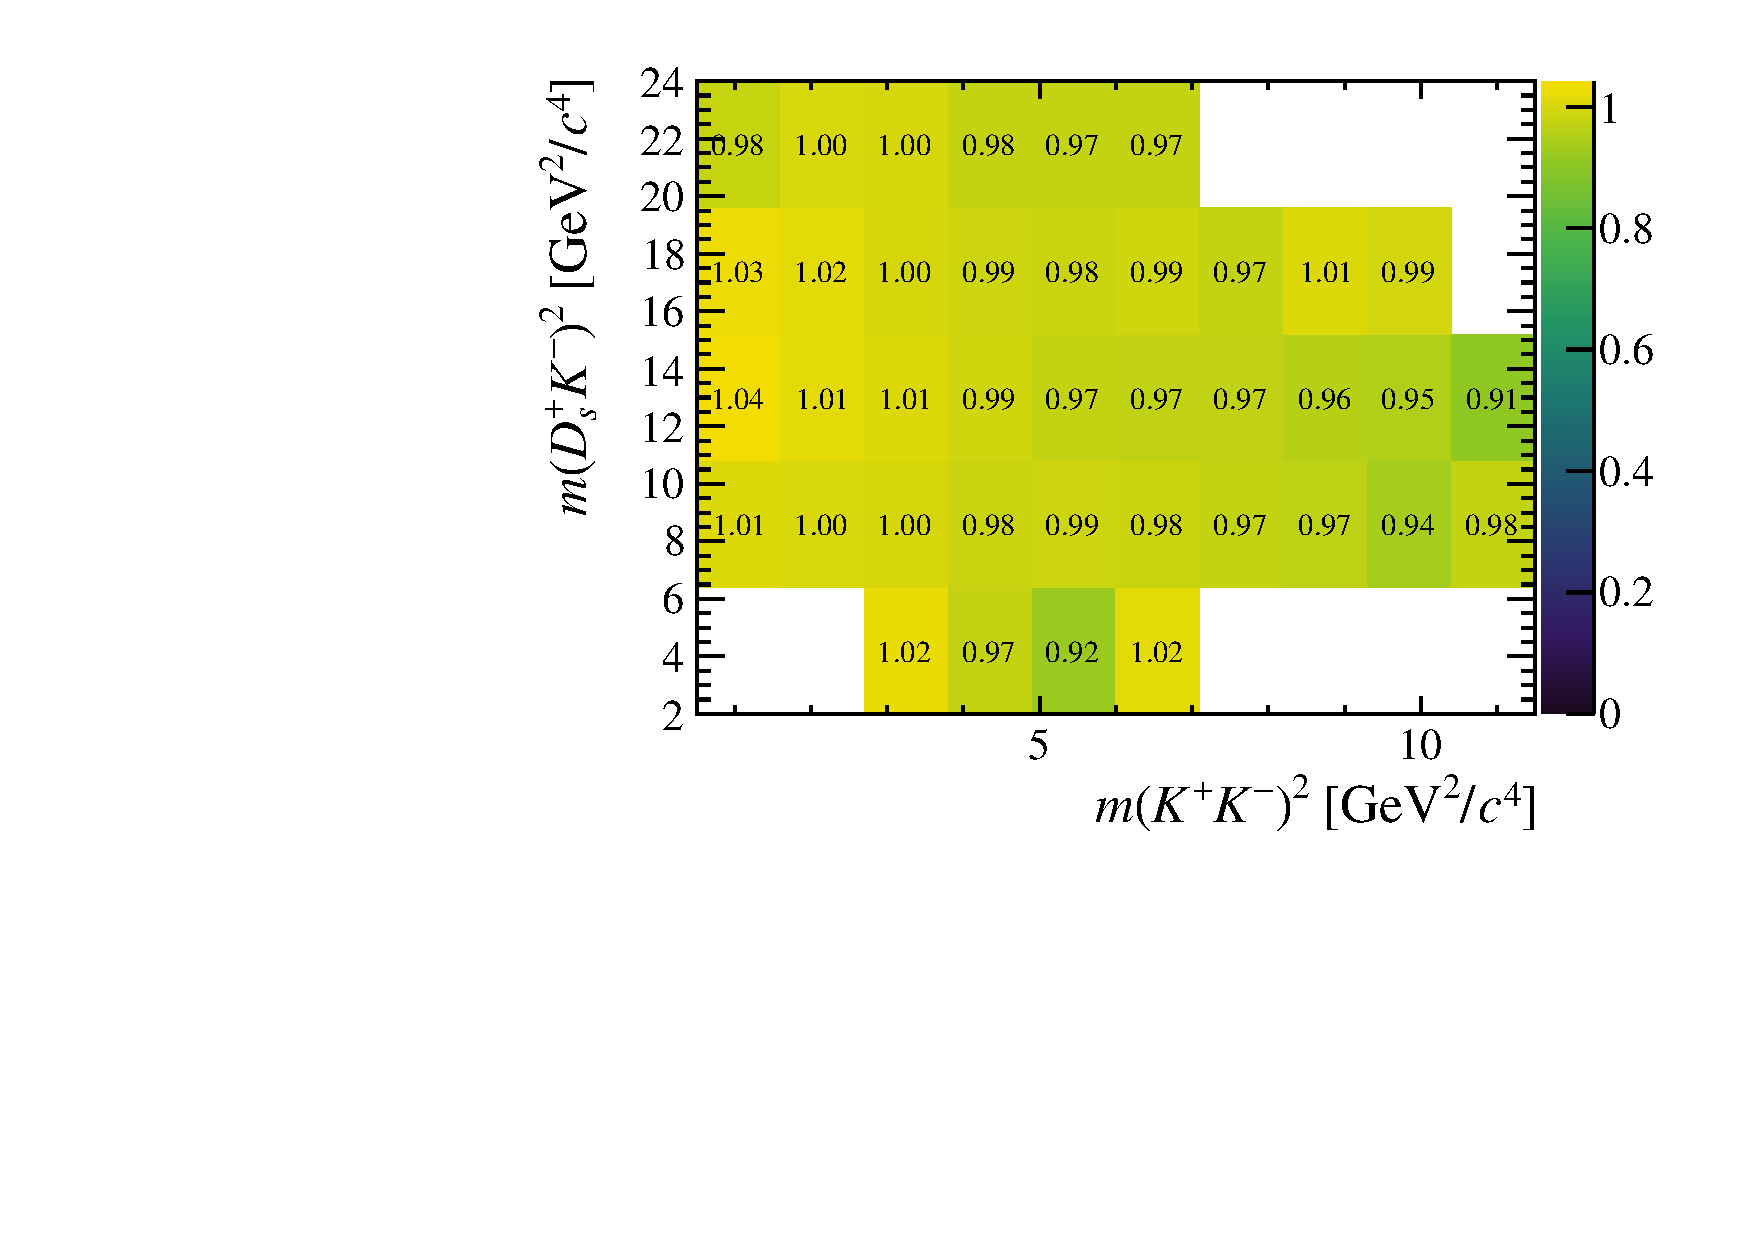
\includegraphics[width=1.0\textwidth]{figs/B2DsKK/Relative_Eff_PID_All.pdf}
      \caption{PID}
      \label{fig:B2DsKK_releff_PID}
   \end{subfigure}
   \begin{subfigure}[t]{0.4\textwidth}
      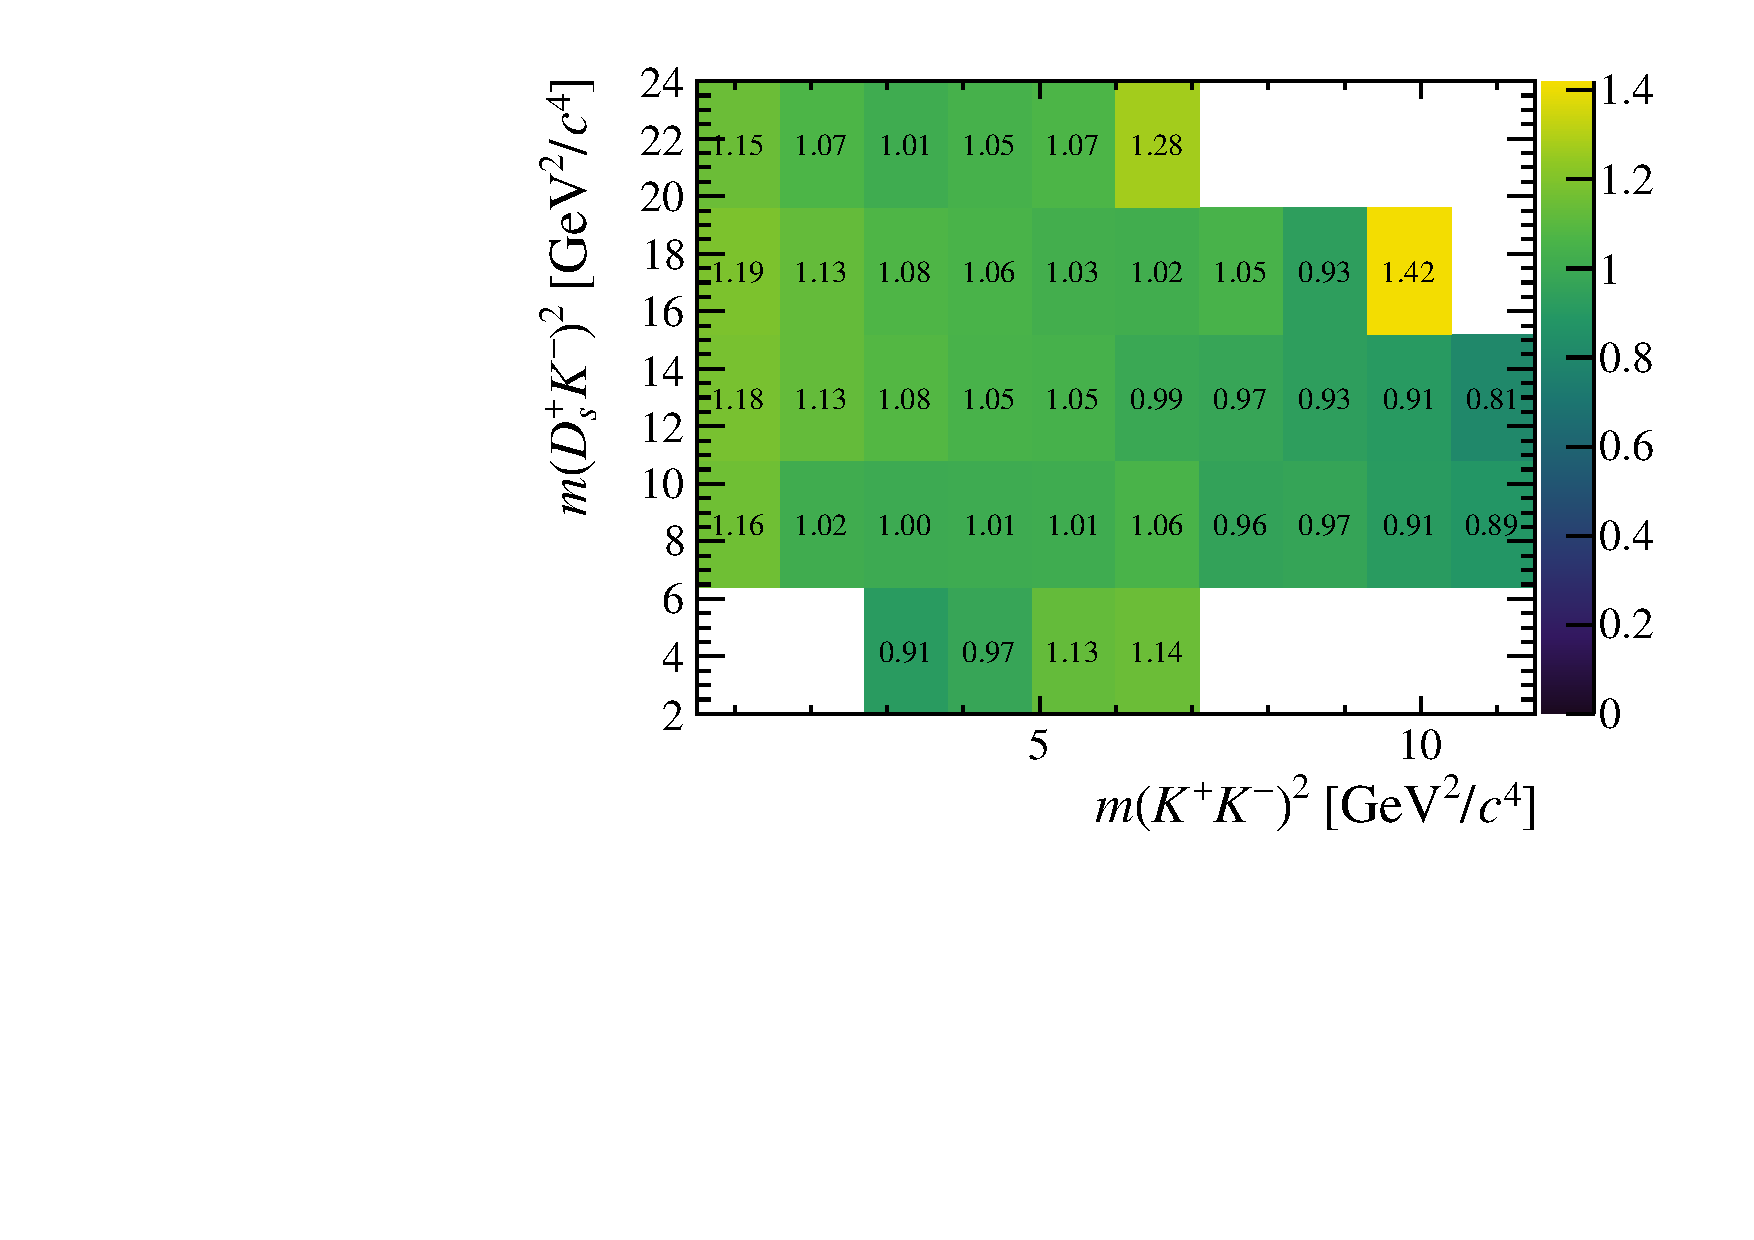
\includegraphics[width=1.0\textwidth]{figs/B2DsKK/Relative_Eff_BDT_All.pdf}
      \caption{MVA}
      \label{fig:B2DsKK_releff_MVA}
   \end{subfigure}
   \caption{The relative efficiency $\epsilon_{\text{ratio}}(m^{2}(\Dsp\Km),m^{2}(\Kp\Km))$ as a function of the \decay{\Bp}{\Dsp\Kp\Km} kinematics.}
   \label{fig:B2DsKK_dalitz_eff_three}
\end{figure}
%%%%%%%%%%%%%%%%%%%%%%%%%%%%%%%%%%%%%%%%%%%%%%%%%%%%%%%%%%



\subsubsection{MVA efficiency}
\label
The relative MVA efficiency shown in Fig.\ref{fig:B2DsKK_releff_MVA} is determined from simulations in which the PID distributions have been corrected to account for the variation in the \Dsp and \phiz MVA efficiency across the phase-space. 
%The corrected PID variables are used to determine the \Dsp and \phiz MVA classifiers and the efficiency of the MVA requirements determined in different positions in the Dalitz plot as shown in Fig.\ref{fig:B2DsKK_releff_MVA}. 
There is a strong dependence on the position in phase-space, with decays at low $m^{2}(\Kp\Km)$ values having a larger relative efficiency than those at higher values. The MVA methods were trained using a sample of \decay{\phiz}{\Kp\Km} decays, so the selection favourably selects candidates near the \phiz-meson mass. 

A crosschecks is performed to compare these MVA efficiencies and the method described in Sec.~\ref{sec:selection_MVA_eff} that uses the MVA training samples to calculate the efficiency. A good agreement is found, however the possible resulting systematic uncertainty is quantified in Sec.~\ref{sec:B2DsKK_sys_releff}.


% The values of the efficiency determined for each mode are compared in Fig.~\ref{fig:B2DsKK_PID_eff_crosscheck} as a function of the $m(\Kp\Km)$ mass. The MVA training modes only exist for two discrete values; $m(\Kp\Km)=m(\phiz)$ and $m(\Kp\Km)=m(\Dzb)$ represented by the red points. These are compared to the \decay{\Bp}{\Dsp\Kp\Km} and \decay{\Bp}{\Ds\Dzb} efficiencies from the corrected simulations in black and blue respectively. A good agreement is found.

% %%%%%%%%%%%%%%%%%%%%%%%%%%%%%%%%%%%%%%%%%%%%%%%%%%%%%%%%%%
% \begin{figure}[!h]
%    \centering
%    \begin{subfigure}[t]{0.49\textwidth}
%       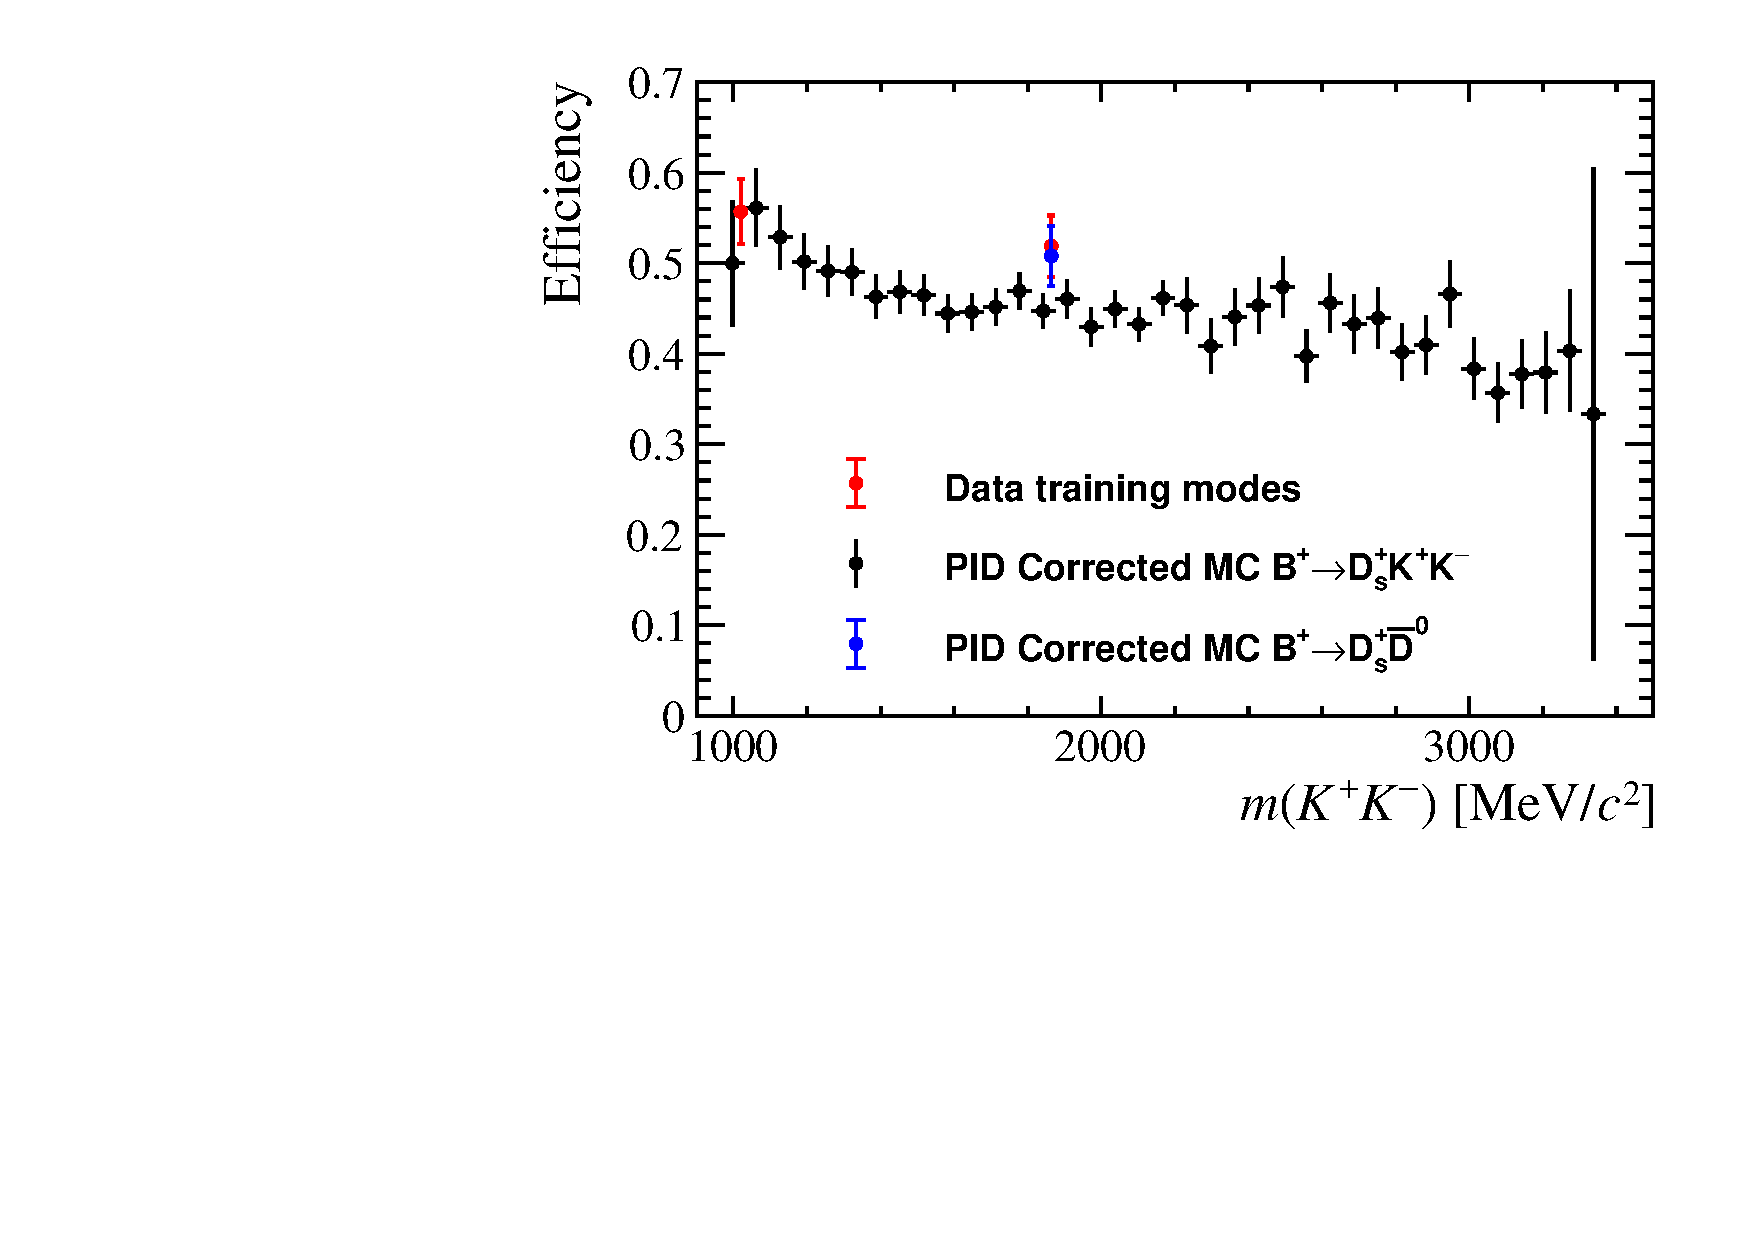
\includegraphics[width=1.0\textwidth]{figs/B2DsKK/mKK_eff_2011_Both.pdf}
%       \caption{2011}
%    \end{subfigure}
%    \begin{subfigure}[t]{0.49\textwidth}
%       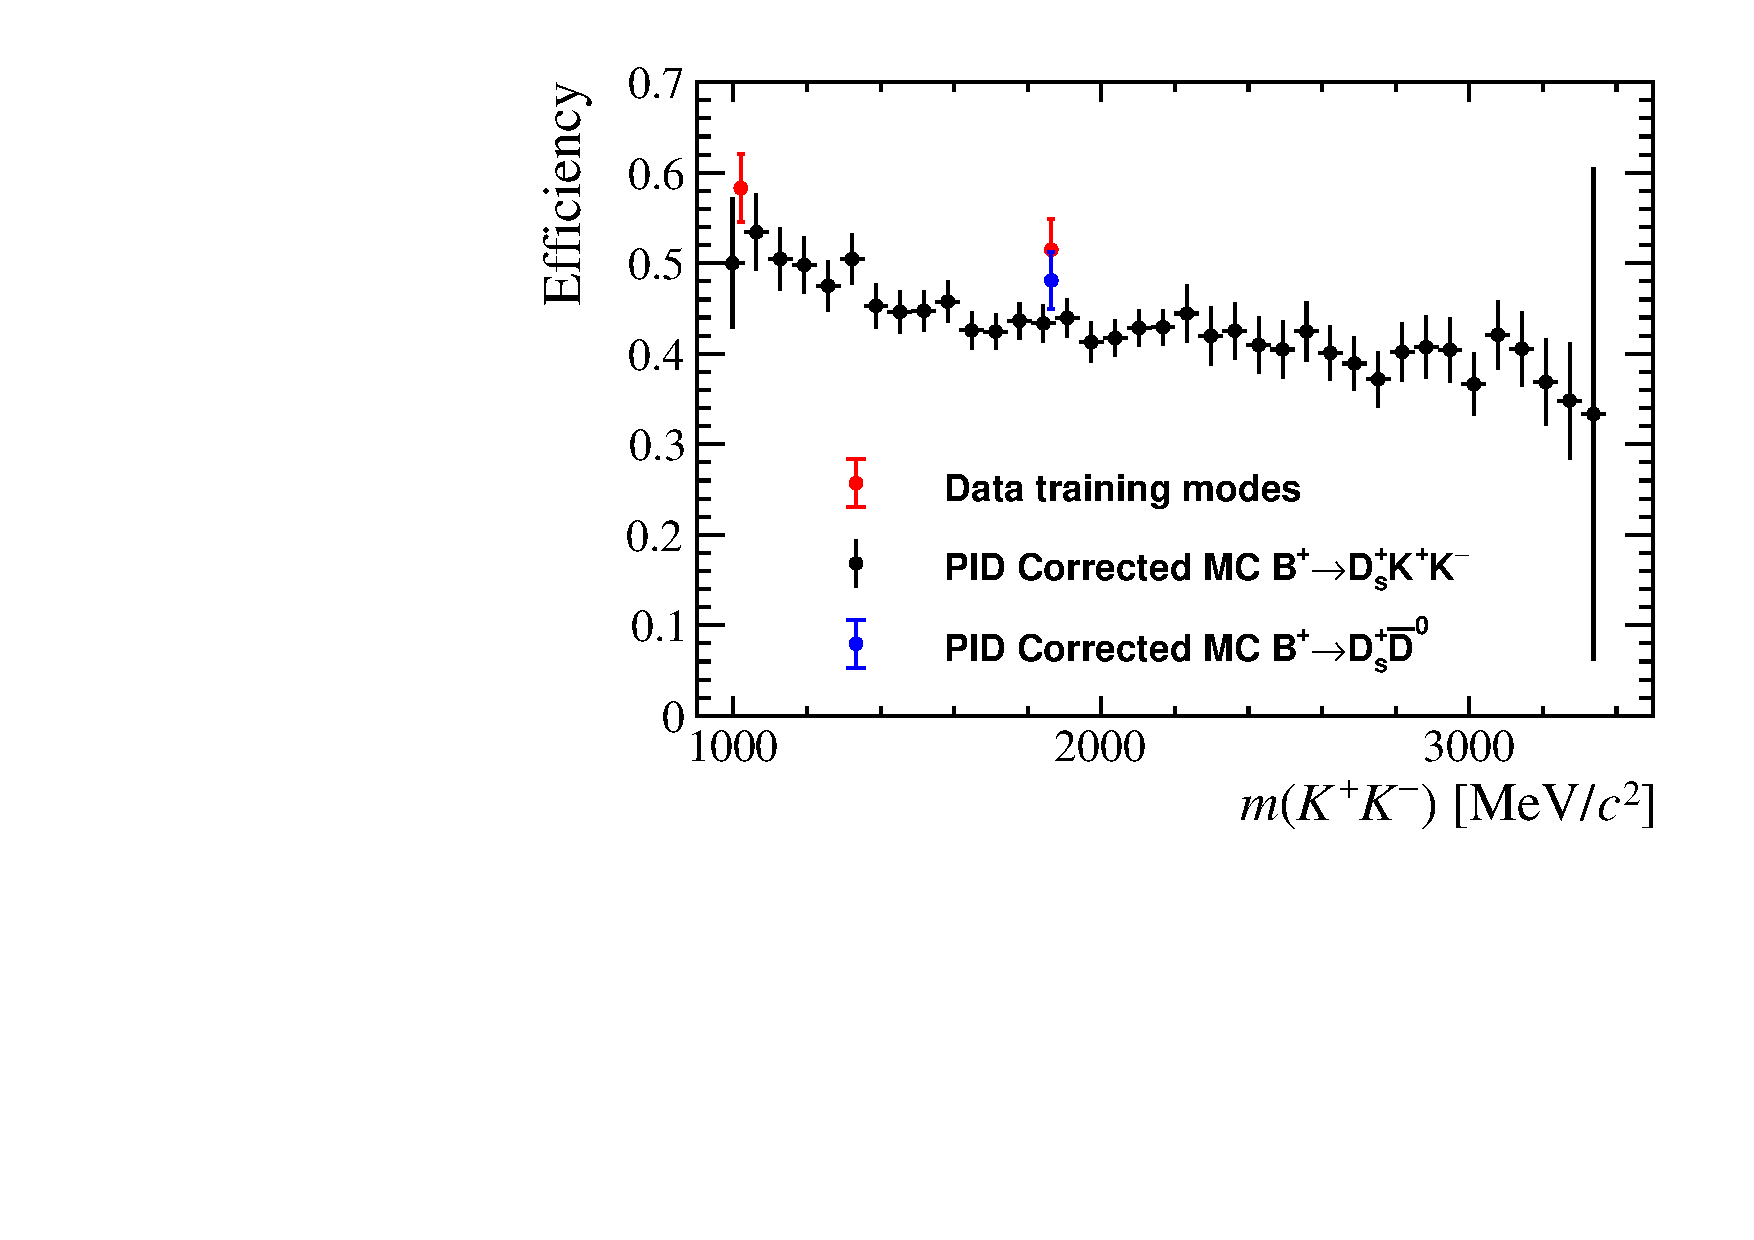
\includegraphics[width=1.0\textwidth]{figs/B2DsKK/mKK_eff_2012_Both.pdf}
%       \caption{2012}
%    \end{subfigure}
%    \caption{The PID efficiency variation as a function $m(\Kp\Km)$ as determined from the MVA training modes (red) and the \decay{\Bp}{\Dsp\Kp\Km} and \decay{\Bp}{\Ds\Dzb} simulation samples (black and blue respectively). A good agreement is found between the red and black point at $m(\Kp\Km)=m(\phiz)$, and the red and blue point at $m(\Kp\Km)=m(\Dzb)$.}
%    \label{fig:B2DsKK_PID_eff_crosscheck}
% \end{figure}
% %%%%%%%%%%%%%%%%%%%%%%%%%%%%%%%%%%%%%%%%%%%%%%%%%%%%%%%%%%




\subsection{Total efficiency}
The total relative efficiency between the signal and normalisation decays is calculated from the products of each contributing efficiency
\begin{multline}
\epsilon^\text{Tot.} = \epsilon^{\text{Accp.}} \times \epsilon^{\text{Reco.}|\text{Accp.}} \times \epsilon^{\text{Trig.}|\text{Reco.}}\times \epsilon^{\text{Mass.}|\text{Trig.}}\times \epsilon^{\text{Veto.}|\text{Mass.}}\times \epsilon^{\text{FD}|\text{Veto.}}\\
\times \epsilon^{\text{IP}|\text{FD}} \times \epsilon^{\text{PID}|\text{IP}} \times \epsilon^{\text{MVA}|\text{PID}},
\label{eq:B2DsPhi_eff_eq}
\end{multline}
where each relative efficiency $x$ is defined relative to the previous selection step $y$ as $\epsilon^{x|y}$. This is determined as a function of the two-dimensional $m^{2}(\Dsp\Km)$ vs. $m^{2}(\Kp\Km)$ space and shown in Fig.~\ref{fig:B2DsKK_eff_total_hist}. 
%This two dimensional histogram has a coarse binning and is susceptible to variations from statistical fluctuation.  
%This could lead to biases when correcting the weights of signal candidates, especially if the candidates are concentrated within a one or a few bins. To reduce this 
The two dimensional histogram is made into a smoothly varying distribution by using a cubic spline interpolation as shown in Fig.~\ref{fig:B2DsKK_eff_total_spline}. The final distribution used to correct the yields of signal decays is the weighted sum of the splines for each year of data taking.


%%%%%%%%%%%%%%%%%%%%%%%%%%%%%%%%%%%%%%%%%%%%%%%%%%%%%%%%%%
\begin{figure}[!h]
   \centering
   \begin{subfigure}[t]{0.4\textwidth}
      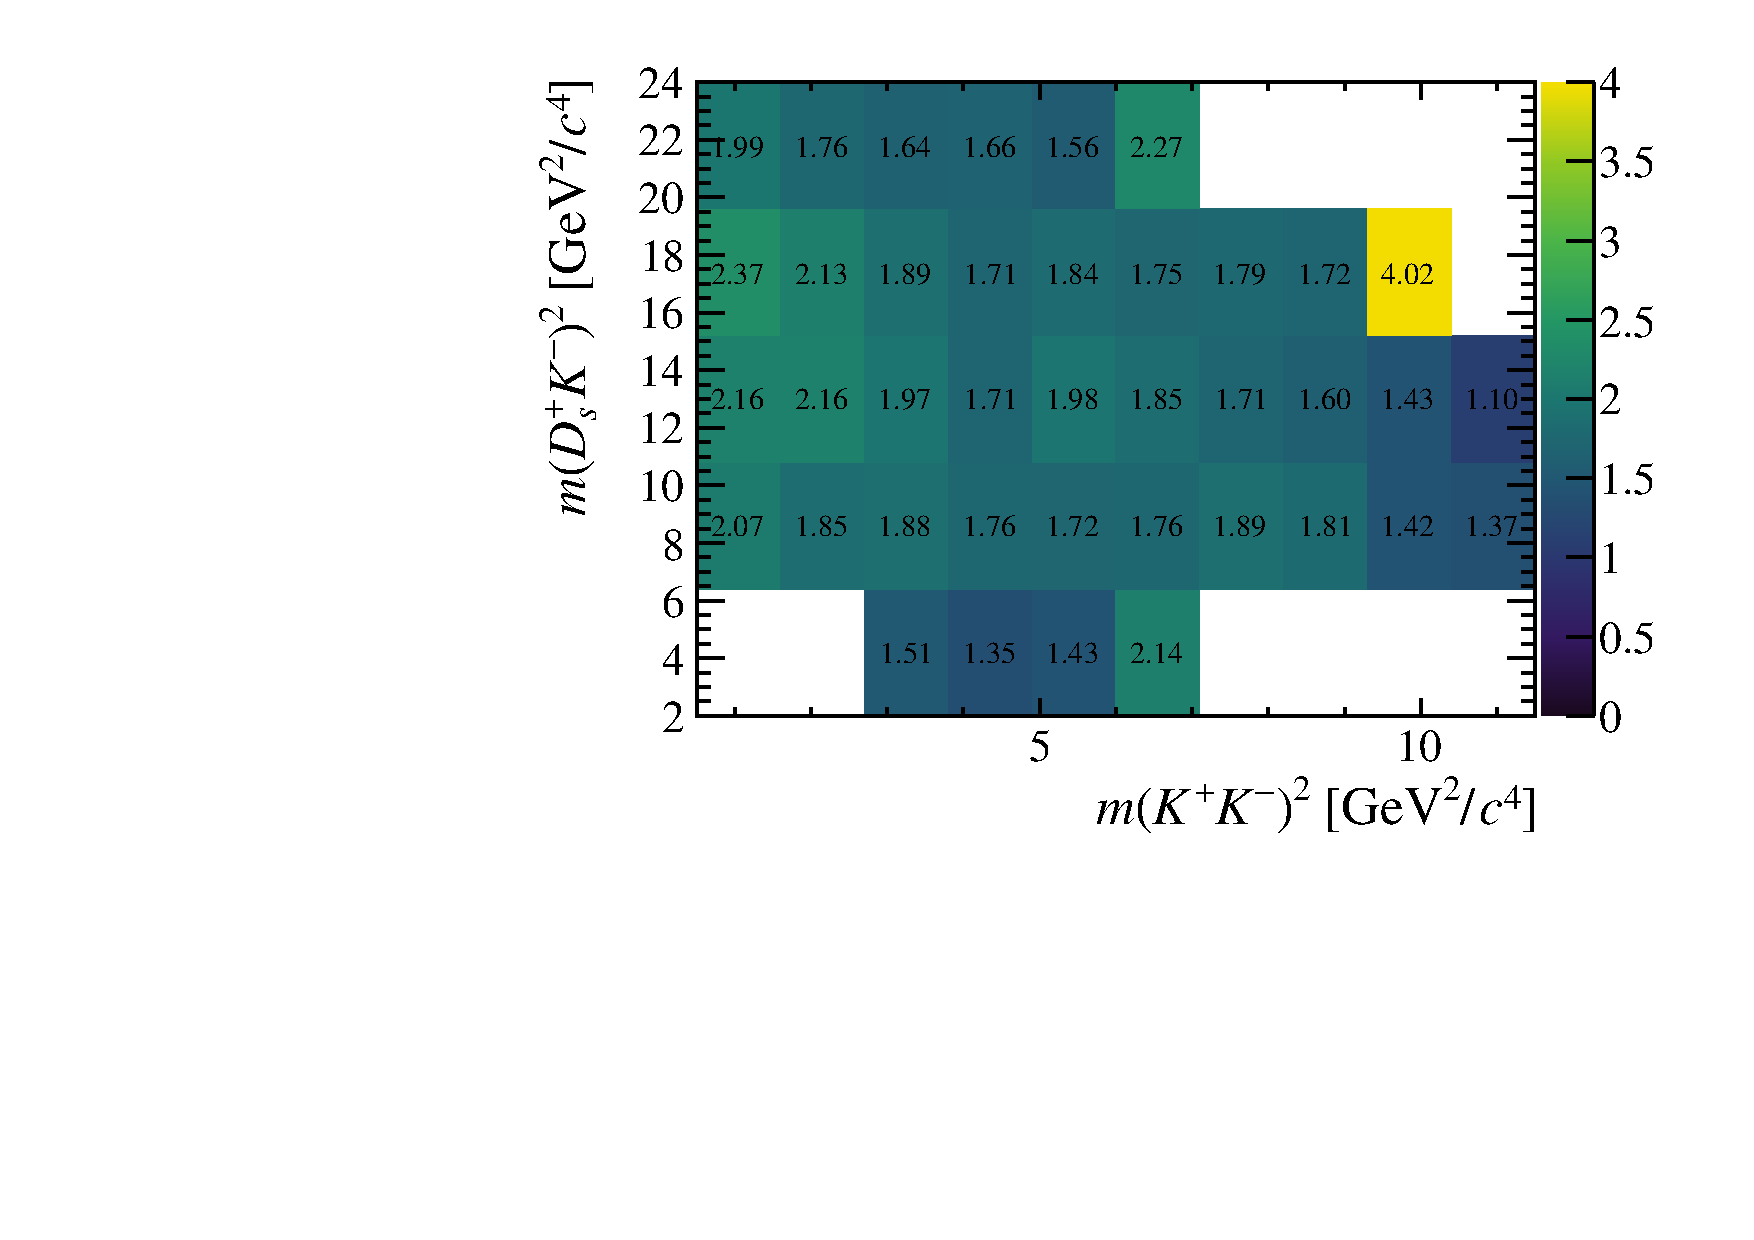
\includegraphics[width=1.0\textwidth]{figs/B2DsKK/Full_Eff_Hist_All.pdf}
      \caption{Total efficiency}
      \label{fig:B2DsKK_eff_total_hist}
   \end{subfigure}
   \begin{subfigure}[t]{0.4\textwidth}
      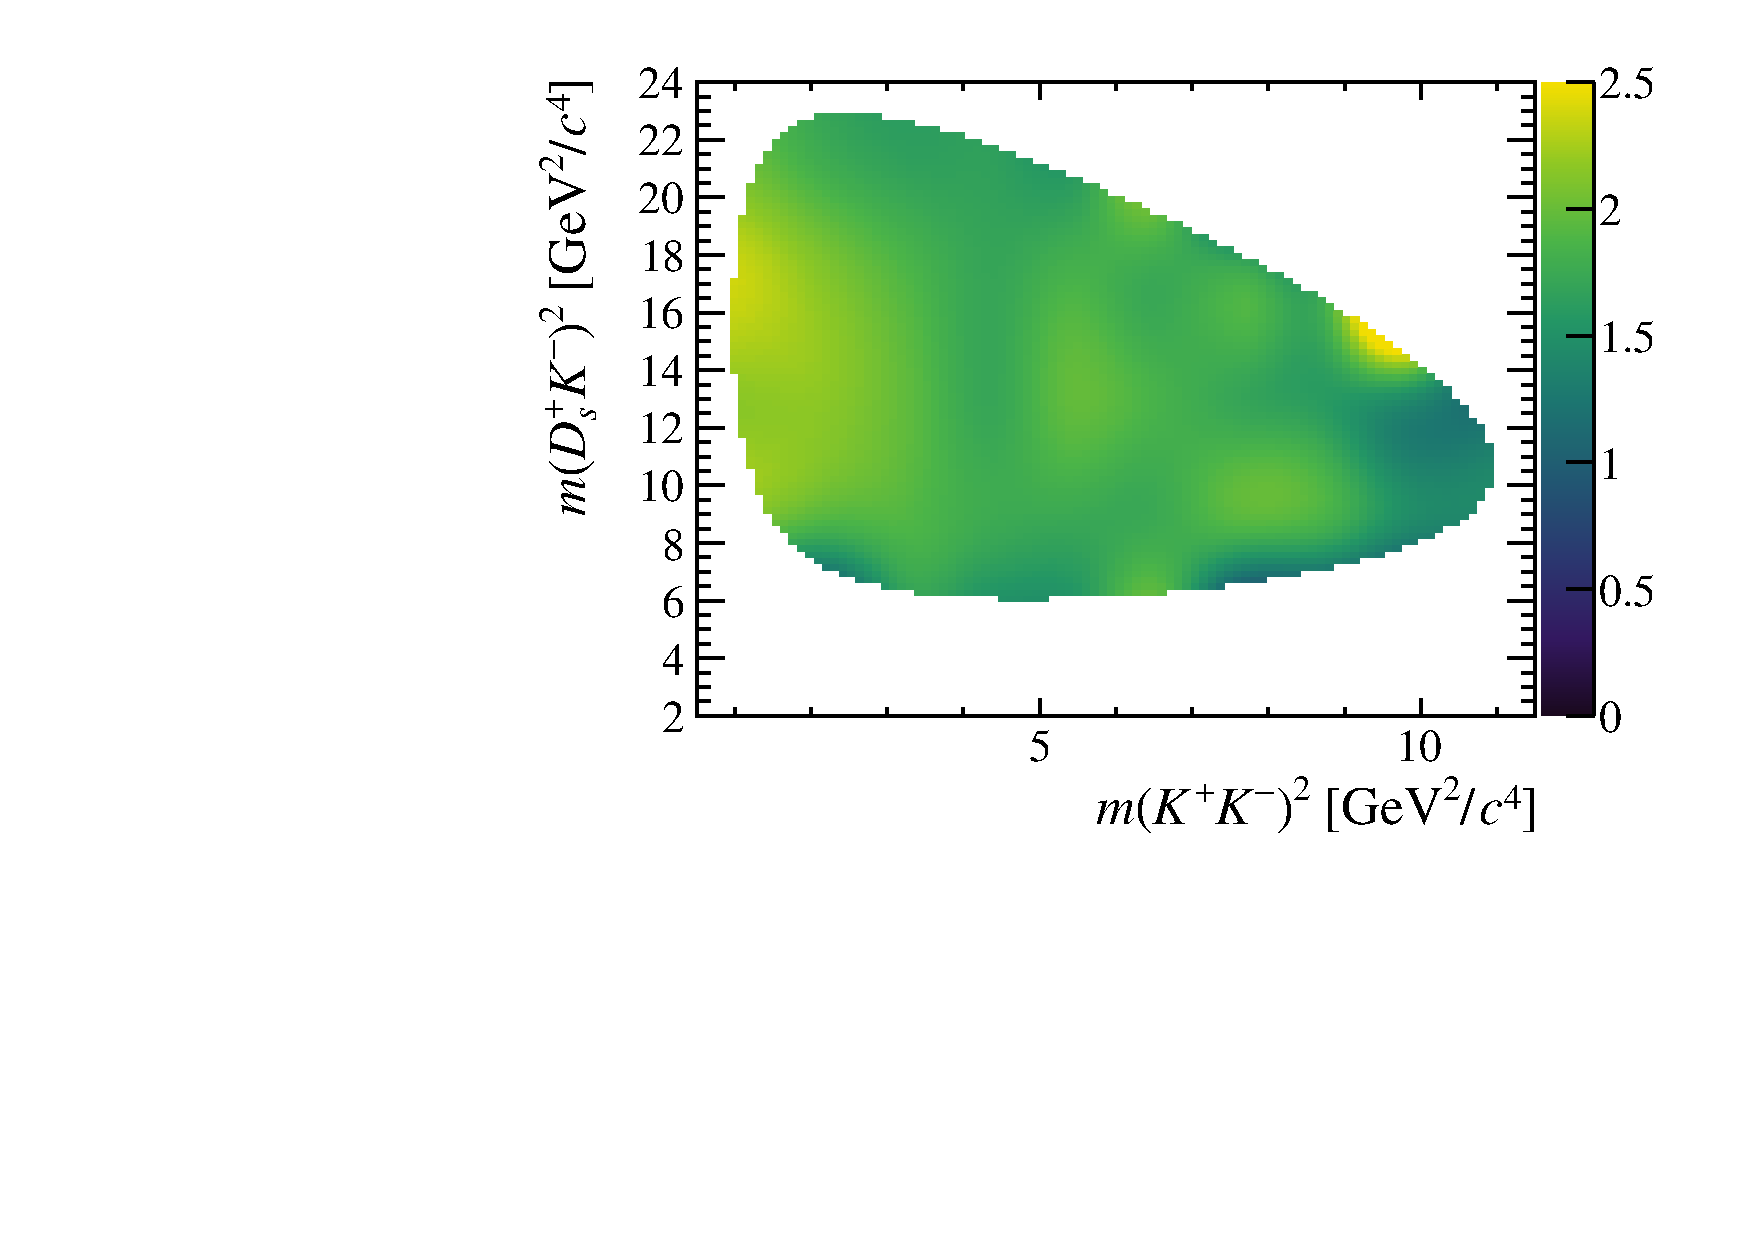
\includegraphics[width=1.0\textwidth]{figs/B2DsKK/Full_Eff_Spline_All_withLimit.pdf}
      \caption{Spline interpolation}
      \label{fig:B2DsKK_eff_total_spline}
   \end{subfigure}
   \caption{The total relative efficiency $\epsilon_{\text{ratio}}(m^{2}(\Dsp\Km),m^{2}(\Kp\Km))$ between the signal and normalisation mode as a function of the two-dimensional $m^{2}(\Dsp\Km)$ vs. $m^{2}(\Kp\Km)$ (left) and a cubic spline interpolation of the same distribution (right).}
   \label{fig:B2DsKK_total_eff}
\end{figure}
%%%%%%%%%%%%%%%%%%%%%%%%%%%%%%%%%%%%%%%%%%%%%%%%%%%%%%%%%%


\section{Systematic uncertainties}
\label{sec:B2DsKK_systuncertainy}


A number of sources of systematic uncertainty are considered when determining the branching fraction for \decay{\Bp}{\Dsp\Kp\Km} decays.



\subsection{Relative efficiencies}
\label{sec:B2DsKK_sys_releff}

The yields of signal and normalisation decays are corrected by the ratio of selection efficiencies. The limitations and assumptions surrounding this ratio contribute to the systematic uncertainty.

\begin{description}
\item \textbf{Simulation statistics:} the relative efficiencies used in this analysis are determined from limited simulation samples resulting in an uncertainty of 2\%. 

\item \textbf{Particle identification:} the procedure used to determine the PID efficiencies introduces sources of systematic uncertainty, for example the choice of binning scheme used to match the calibration samples to the signal decays and the background-subtraction procedure used to isolate the distributions. 
%The presence of the same particle species in the signal and normalisation mode helps to reduce this effect in the ratio of efficiencies. 
A conservative uncertainty of 0.5\% per track is assigned to any residual differences. This is assumed to be uncorrelated for the five signal and five normalisation tracks, resulting in a total relative uncertainty of 2.0\%.

\item \textbf{Veto efficiency:} the efficiency of the misidentified \Dp and \Lc hadron vetoes applied to the \Dsp meson is assumed to be the same for the signal and normalisation channel. However, slight differences in the kinematics of the \Dsp mesons in each case might lead to this approximation not being valid. An uncertainty of 1.4\% is assigned to account for any bias.
% when the particle identification requirements are tightened on the ambiguous track. The relative veto efficiency could be calculated by determining the relative PID efficiency for the sub-set of particles that would be affected by the tightening of the cuts. Rather than calculating this ratio, an uncertainty of 1.4\% is assigned to account for any bias.   

\item \textbf{MVA efficiency:} the relative MVA efficiency receives contributions from a number of sources.
They are determined from corrected simulations samples (Sec.~\ref{sec:B2DsKK_eff_from_calib}) using Run I calibrations. The phase-space distributions in Run I and Run II are assumed to be the same, whilst the absolute values of the efficiencies are scaled using input from the calibration samples \decay{\Bs}{\jpsi\phiz} and \decay{\Bsb}{\Dsp\pim}. An uncertainty of 4.4\% is associated to this assumption. 
The data-driven efficiencies obtained from the \decay{\Bs}{\jpsi\phiz} and \decay{\Bsb}{\Dsp\pim} samples are associated to uncertainties as a result of the choice of binning scheme and finite sample sizes. 
The uncertainty arising from differences in simulation and data distributions that could affect the MVA efficiencies (Fig.~\ref{fig:ipchi2dist_normalisation} and Fig.~\ref{fig:mvaclassifierresponses}) are also taken into account.
The total systematic uncertainty associated to the relative MVA efficiency is 7.6\%. 


%%%%%%%%=====> 
% the relative efficiency of the MVA selection receives contributions from a number of sources. Primarily, the relative efficiencies are determined from simulation samples in which the PID variable distributions have been corrected as described in Sec.~\ref{sec:B2DsKK_eff_from_calib}. This method of correcting the PID distributions such that the simulation samples could be used directly was only available for Run I simulations at the time of analysis. The phase-space distributions of the Run II samples were assumed to be the same, but the overall scale adjusted using the MVA efficiencies derived from the \decay{\Bs}{\jpsi\phiz} and \decay{\Bsb}{\Dsp\pim} decay modes used to train the MVAs. The systematic uncertainty arising from using the Run I variations in Run II are estimated by calculating the largest difference between the signal and normalisation efficiencies in Run II and subtracting the smallest differences in Run I. This corresponds to a variation of 4.4\%, assigned as the systematic uncertainty.

% As they contribute to the scaling of the phase-space variations, all sourced of systematic uncertainty contributing to the data-driven efficiencies are also considered. The training modes are binned in four bins of \pt and $\chi^{2}_{\text{FD}}$. The choice of binning scheme is varied and the resulting variation in efficiency determined. The yields of the \decay{\Bs}{\jpsi\phiz} and \decay{\Bsb}{\Dsp\pim} decays used to obtain the data-driven efficiencies are limited, therefore the quantity $1/\sqrt{N}$ associated to the smallest of these yields is added as a systematic uncertainty. 

% Differences are observed in the distribution of $\chi^{2}_{\text{IP}}$ in simulations and data for the normalisation channel (Fig.~\ref{fig:ipchi2dist_normalisation}). To quantify the effect this may have on the MVA efficiencies, the simulations are re-weighted to match the data distributions and the efficiencies recalculated. The resulting difference is included as a systematic uncertainty.

% When training the MVA methods some discrepancies are observed between the MVA classifier response for the training and validations samples (Fig.~\ref{fig:mvaclassifierresponses}). To assess whether this affects the final relative MVA efficiencies the training and validation samples are swapped and the efficiencies recalculated. The differences for each year of data taking are weighted according to their contribution to the final data set and assigned as a systematic uncertainty.  

% - binning scheme
% - yields of eff samples
% - training testing discrepancies
% - MVA classifier differences between norm and eff modes
% - Run 1 as Run 2
\end{description}

% {\color{Blue}
% \begin{description}

% \item \textbf{BDT Efficiency Ratio} All of the sources of systematic uncertainty associated with the BDT efficiency ratio still apply here, particularly as the data trained efficiencies are still used to find the ratio in Run 2. 

% - An additional systematic is assigned to account for the use Run 1 Dalitz plot dependences on the BDT and PID ratios. We assume the shapes of the Dalitz plot dependences are the same for Run 1 and Run 2, but adjust the overall scale to match the efficiencies determined previously. However by looking at the differences between the efficiencies for $\B \to \Ds \Dz$ and $\B \to \Ds \phi$ in Table~\ref{tab:BDT}, one sees that the differences get larger in Run 2, implying the shape may indeed get steeper. As a very conservative estimate we take the largest difference between $\B \to \Ds \Dz$ and $\B \to \Ds \phi$ in Run 2 and subtract the smallest difference in Run 1. This gives a difference of 4.4\% which we assign as the systematic uncertainty. This is likely to be an overestimate of the effect on the final branching fraction as most of the signal events are found in a small area of the phase-space, leading to smaller variations in efficiency. This systematic can be removed if support for Run 2 in \texttt{Meerkat}/\texttt{PIDCorr} becomes available before publishing.


% - The calculation of the BDT efficiency has a systematic uncertainty due to the choice of binning scheme used to match the signal and training kinematics. The bins were chosen to have equal occupancy in each of the two variables in the BDT training modes. Varying the bin size by 20\% results in a change in the relative BDT efficiency of 2\%. 

% - Additionally uncertainty arises due to the use of finite reference samples. The yields of each particle used to obtain the efficiencies are listed in Table~\ref{table:mva_training_yields}. Half of these samples are used for BDT training, and the other half for testing. The smallest sample is that of $\phi \to KK$ where there are $12.7k$ $\phi$ mesons in the testing sample. We apply a 1\% systematic uncertainty to account for this finite sample size by assuming the relative statistical errors associated with a finite sample are proportional to $1/\sqrt{N}$. 

% - It is observed that there are discrepancies in the distributions of MVA response between the training and testing samples used by some of the MVAs in this analysis (see Appendix~\ref{sec:MVAtraining}). In order to quantify the extend to which these discrepancies might affect the measured branching fraction, we recalculate the BDT efficiencies for the optimised cut values using the training sample instead of the testing sample. For most \Ds decay modes and years the resulting change is very small. The largest changes are for $\Ds \to K\pi\pi$ where in 2011 and 2016 data the efficiencies for the signal and normalisation both rise by around $\sim$5\%. However, as both the normalisation channel and signal channel are affected in the same way, the change in the ratio is suppressed. A total systematic uncertainty is calculated by weighting the change in the ratio for each sub-sample by the fraction of total normalisation mode events observed in that sub-sample. This leads to a total change of $\sim$0.5\% in the weighted BDT efficiency ratio.

% - There are some difference in the MVA classifer for the reweighted data training modes and the normalisation peaks as observed in Fig.~\ref{fig:mvaresponse}, particularly in the mode $\Ds \to \pi \pi \pi$ in Run 2. Additionally, difference are observed in the MC and data distributions of the \B meson impact parameter significance in Fig.~\ref{fig:IPCHI2_cuts_norm}. To determine what effect any mismodelling might have on the calculated BDT efficiencies, the signal and normalisation MC samples are reweighted to match the distributions in data of \B $\chi^{2}_{IP}$. The largest variation in the ratio of BDT efficiencies is for the sample of $\Ds \to \pi \pi \pi$, which changes by 2.7\%. When the change in all samples is weighted according to their relative contribution to the total dataset the variation is 0.9\%. The larger of these two variations is added as a systematic uncertainty for this effect. 
% The total BDT efficiency systematic uncertainty is the sum of these effects, totalling 6.2\%.

% \end{description}
% }

\subsection{Signal and normalisation PDFs}

Some parameters in the signal and normalisation PDFs are fixed to values obtained from simulation. These include the tail parameters, relative widths, and fractional amounts of the two CB functions that make up the PDFs. The values obtained from simulation have associated uncertainties arising from the limited simulation sample sizes. The nominal fits are repeated with the fixed parameters modified to values sampled from Gaussian distributions, with a width given by the parameter uncertainties. All parameters are changed simultaneously. The resulting variation of 0.5\% is assigned as the associated systematic uncertainty. 

\subsection{Background PDFs}

In the signal mode the PDFs for the partially reconstructed background modes are taken directly from simulated events using one-dimensional kernel estimations~\cite{Cranmer:2000du}. In the nominal fit, these are smeared to account for the differences in the mass resolution between data and simulation. To account for any systematic uncertainty arising from the choice of resolution difference, the fit is repeated, randomly varying the smearing resolution each time. The resulting variation in the branching fraction is assigned as a systematic uncertainty. 

In the normalisation mode a number of choices are made about the partially reconstructed backgrounds, namely the kinematic limits of the \decay{\Bp}{\Dssp\Dzb} and \decay{\Bp}{\Dsp\Dstarzb}, and the external branching fractions of \decay{\Dssp}{\Dsp[\Pgamma/\piz]},
 \decay{\Dstarzb}{\Dzb[\Pgamma/\piz]} decays. These assumptions are simultaneously varied within the relevant uncertainties, resulting in a change of 0.2\% in the branching fraction.



\subsection{Charmless contribution}

The residual `charmless' (not a true \Dsp) contribution is only a significant fraction of the measured yield for the normalisation mode (Table~\ref{tab:selection_fd_cuts}). The residual yield of about eight candidates expected in the final selection corresponds to a relative difference of 0.7\% of the measured normalisation yield. However, the constrained \Dsp mass smears the charmless candidates over a wider range so reduces this peaking background.
A systematic uncertainty on the branching fraction of 0.7\% is assigned.

% Rather than trying to include a PDF for this contribution or correcting the measured yield the expected size of the effect is used as the systematic uncertainty as it would propagate directly to the branching fraction. 


\subsection{Total systematic uncertainty}
The systematic uncertainties contributed from each source discussed is detailed in Table~\ref{table:B2DsKK_systematics}. The total systematic uncertainty is also shown, along with the uncertainty arising from the externally measured normalisation channel branching fractions. 

\begin{table}[!ht]
    \centering
    \begin{tabular}{  l   c   c }
        \hline
        \multirow{ 2}{*}{\textbf{Source of Uncertainty} }&\multicolumn{2}{ c }{ Systematic Uncertainty}           \\
                                                         &\textbf{Relative} & \textbf{Absolute ($\times 10^{-6}$)}\\
        \hline 
        MVA relative efficiency                     & 7.6\% & $0.53$\\
        %BDT Relative efficiency                     & 6.2\% & $0.44$\\
        %Using Run 1 shapes as Run 2                 & 4.4\% & $0.31$\\
        Simulation statistics                       & 2.0\% & $0.14$\\
        PID relative efficiency                     & 2.0\% & $0.14$\\
        Veto relative efficiency                    & 1.4\% & $0.10$\\
        Charmless contribution                      & 0.7\% & $0.05$\\
        Signal PDF parametrisation                  & 0.5\% & $0.04$  \\
        Background PDF parametrisation              & 0.2\% & $0.02$  \\
        \hline
        Total                                       & 8.5\% & $0.59$\\
        \hline
        Normalisation                               & 10.0\% & $0.70$\\
        \hline
    \end{tabular}
    \caption{Contributions to the total systematic uncertainty of the \decay{\Bp}{\Dsp\Kp\Km} branching fraction measurement. The contributions are listed in descending order.}
    \label{table:B2DsKK_systematics}
\end{table}  

\section{Results}
\label{sec:B2DsKK_results}

%%%%%%%%%%%%%%%%%%%%%%%%%%%%%%%
The fit to $\decay{\Bp}{\Dsp\Kp\Km}$ candidates finds a total yield of $N(\decay{\Bp}{\Dsp\Kp\Km}) = 443 \pm 29 $ candidates. 
This is the first observation of this decay mode.
The branching fraction is calculated as
\begin{equation}
\mathcal{B}(\decay{\Bp}{\Dsp\Kp\Km}) = \frac{ N_{\text{corr}}(\decay{\Bp}{\Dsp\Kp\Km}) }{ N(\decay{\Bp}{\Dsp\Dzb}) } \times \mathcal{B}(\decay{\Bp}{\Dsp\Dzb}) \times \mathcal{B}(\decay{\Dzb}{\Kp\Km})
\label{eq:DsKKBranchingfraction}
\end{equation}
\noindent where $N(\decay{\Bp}{\Dsp\Dzb})$ is the yield of normalisation decays, and $N_{\text{corr}}(\decay{\Bp}{\Dsp\Kp\Km})$ is defined to be
\begin{equation}
N_{\text{corr}}(\decay{\Bp}{\Dsp\Kp\Km}) =  \sum\limits_{i} \frac{W_{i}}{\epsilon^{\text{ratio}}_{i}},
\end{equation}
\noindent where $W_{i}$ is the per-candidate weight, as determined by the \sPlot technique for candidate $i$; and $\epsilon^{\text{ratio}}_{i}$ represents the relative efficiency of the signal and normalisation modes $\epsilon_{i}(\decay{\Bp}{\Dsp\Kp\Km})/\epsilon(\decay{\Bp}{\Dsp\Dzb})$ in the relevant bin of the $\decay{\Bp}{\Dsp\Kp\Km}$ Dalitz plot as calculated in Sec.~\ref{sec:B2DsKK_effcorrection}.


%The uncertainty of the corrected signal yield is calculated following the same procedure as outlined in the \decay{\Bp}{\Dp\Kp\pim} search analysis note~\cite{Wallace:2010891} and summarised here. 

The uncertainty on the corrected yield, $N_{\text{corr}}(\decay{\Bp}{\Dsp\Kp\Km})$, is, in principle 

\begin{equation}
\sigma(N_{\text{corr}}) =  \sqrt{\sum\limits_{i} \left(\frac{W_{i}}{\epsilon^{\text{ratio}}_{i}} \right)^{2}}.
\end{equation}
However, the fit used to determine the \sWeights only allows the yields to float, as opposed to the nominal fit that has additional floating parameters including the signal position and width. This means that this estimate of the corrected yield uncertainty could neglect the uncertainty due to the shape parameters: \ie the uncertainty calculated from the weights, $\sigma_{\text{yields only}}(N) = \sqrt{\sum{W_{i}^{2}}}$, can be less than the uncertainty returned by the nominal fit, $\sigma_{\text{fit}}(N)$.

To correctly account for this possibility, the uncertainty from the shape parameters is separated from the the total uncertainty: $\sigma_{\text{shape}}(N) = \sqrt{\sigma_{\text{fit}}(N)^{2}-\sigma_{\text{yields only}}(N)^{2}}$.
This extra uncertainty is then scaled by the corrected yield to give the total uncertainty


\begin{equation}
\sigma_{\text{corr}}(N_{\text{corr}}) =  \sqrt{  \sigma(N_{\text{corr}})^{2} +  \left( \frac{N_{\text{corr}}}{N} \sigma_{shape}(N) \right)^{2}}.
\end{equation}
For the nominal fit the uncertainties are summarised in Table~\ref{table:DsKK_fit_errors}.

\begin{table}[!ht]
\centering
\begin{tabular}{  c | c   }
\hline
Uncertainty                             &  Value \\
\hline 
$\sigma(N_{\text{corr}})$               & 13.0\\
$\sigma_{\text{fit}}(N)$                & 29.4\\
$\sigma_{\text{yields only}}(N)$        & 25.4\\
$\sigma_{\text{shape}}(N)$              & 14.7 \\ 
\hline
$\sigma_{\text{corr}}(N_{\text{corr}})$ & 14.9 \\ 
\hline
\end{tabular}
\caption{The various uncertainties as detailed in Section~\ref{sec:B2DsKK_results} and their values in the nominal fit.}
\label{table:DsKK_fit_errors}
\end{table}

The corrected yield ratio can be expressed as the ratio of signal and normalisation branching fractions using Eq.~\ref{eq:DsKKBranchingfraction}. The value is measured to be 
\begin{equation}
\frac{ N_{\text{corr}}(\decay{\Bp}{\Dsp\Kp\Km}) }{ N(\decay{\Bp}{\Dsp\Dzb}) } = \frac{\mathcal{B}(\decay{\Bp}{\Dsp\Kp\Km})}{\mathcal{B}(\decay{\Bp}{\Dsp\Dzb})\mathcal{B}(\decay{\Dzb}{\Kp\Km})}  = 0.197 \pm 0.015 \pm 0.017, 
\end{equation}
where the first uncertainty is statistical, and the second is systematic.

The branching fraction for $\decay{\Bp}{\Dsp\Kp\Km}$ decays is determined to be 

\begin{equation}
\mathcal{B}(\decay{\Bp}{\Dsp\Kp\Km}) = (7.1 \pm 0.5 \pm 0.6 \pm 0.7) \times 10^{-6},
\end{equation}
where the first uncertainty is statistical, the second is systematic and the third from the branching fractions of $\decay{\Dzb}{\Kp\Km}$ and of the normalisation mode $\decay{\Bp}{\Dsp\Dzb}$. 
The values used for the branching fractions are $\mathcal{B}(\decay{\Dz}{\Kp\Km}) = (4.01 \pm 0.07)\times10^{-3}$~\cite{PDG2016} and $\mathcal{B}(\decay{\Bp}{\Dsp\Dzb}) = (9.0 \pm 0.9)\times10^{-3}$~\cite{PDG2016}. 

The measured \decay{\Bp}{\Dsp\Kp\Km} branching fraction is of a comparable magnitude to the decay \decay{\Bp}{\Dsp\piz} that proceeds via a similar process, without an \squark\squarkbar pair produced: $\mathcal{B}(\decay{\Bp}{\Dsp \piz}) = (1.5 \pm 0.5) \times 10^{-5}$~\cite{Aubert:2006xy}.  

\subsection{Dalitz structure}


%%%%%%%%%%%%%%%%%%%%%%%%%%%%%%%%%%%%%%%%%%%%%%%%%%%%%%%%%%
\begin{figure}[!h]
    \centering
    \begin{subfigure}[t]{0.49\textwidth}
        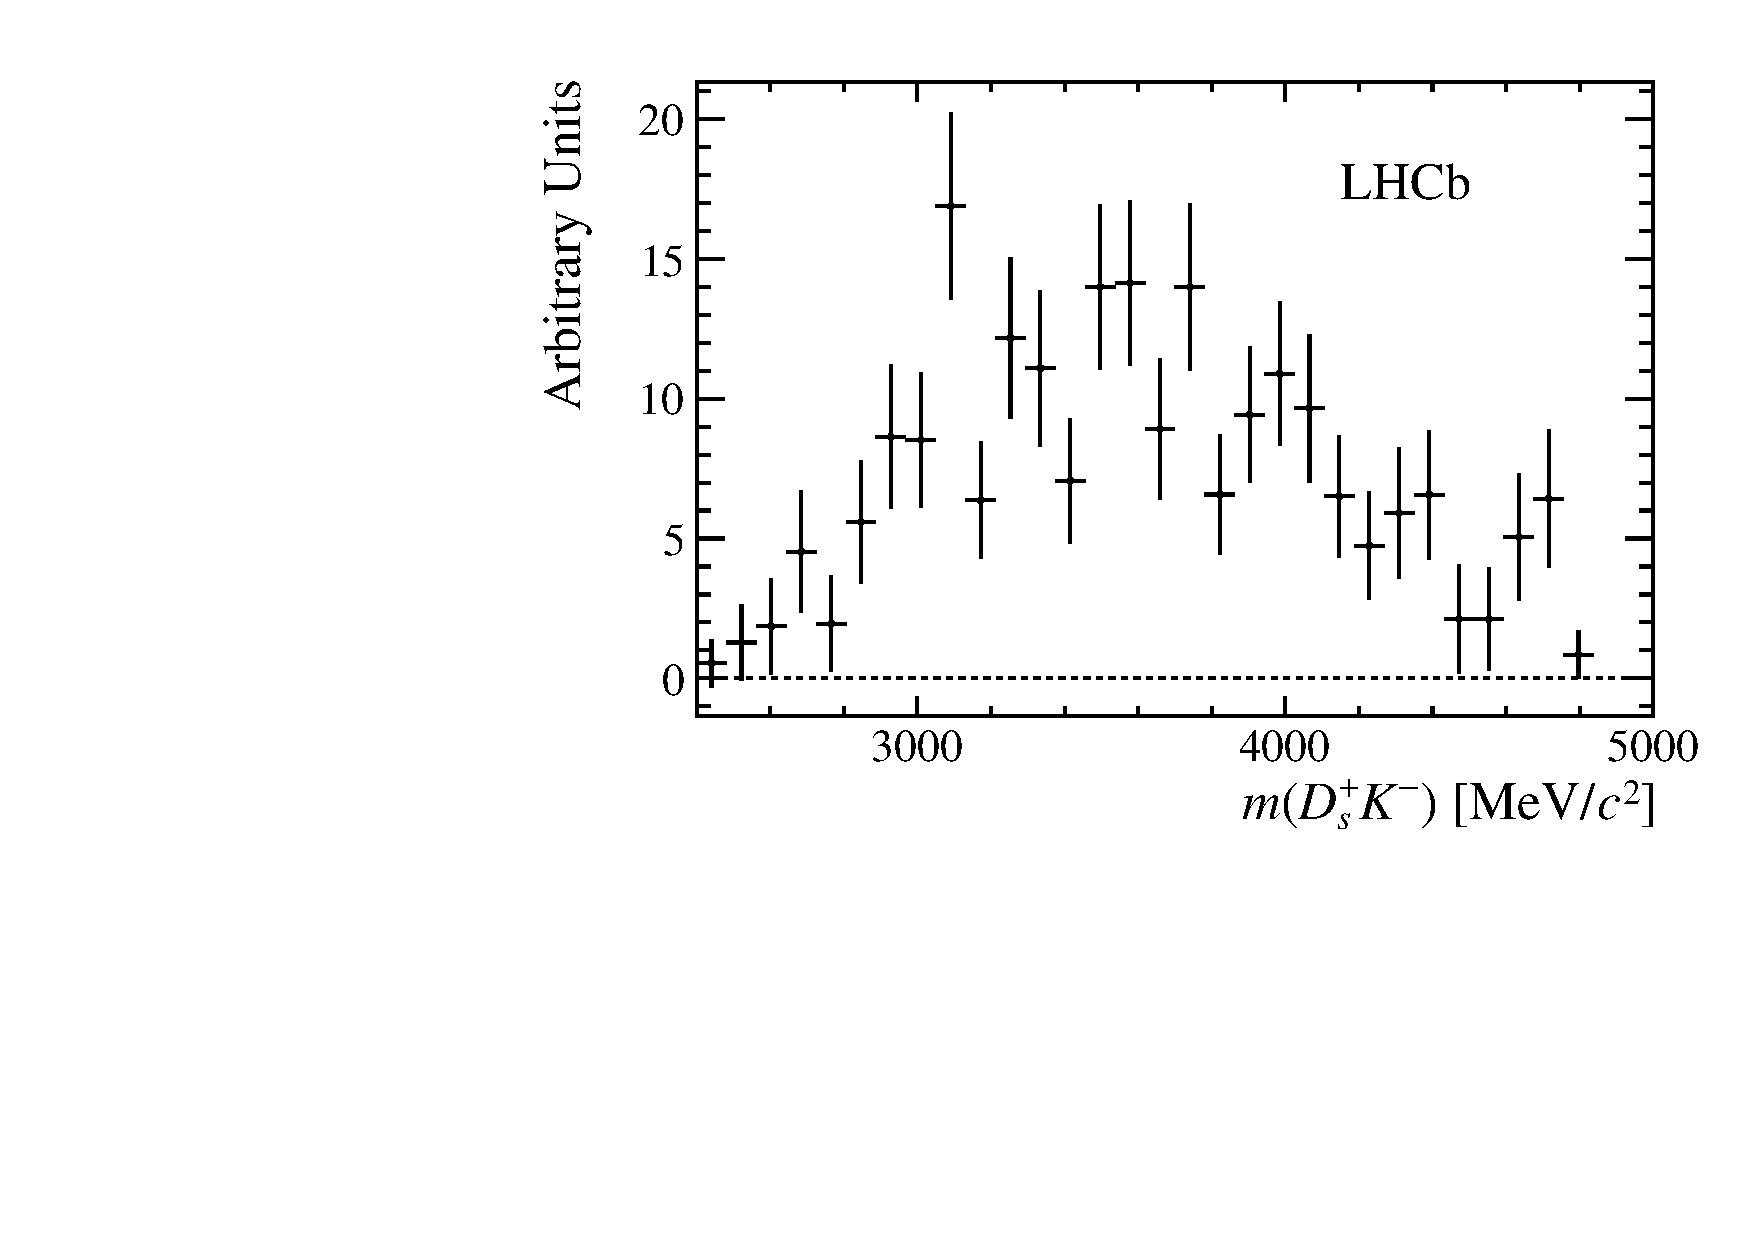
\includegraphics[width=1.0\textwidth]{figs/B2DsKK/DsKm_mass_sweighted.pdf}
        %\caption{Normalisation without selection}
    \end{subfigure}
    % \begin{subfigure}[t]{0.4\textwidth}
    %     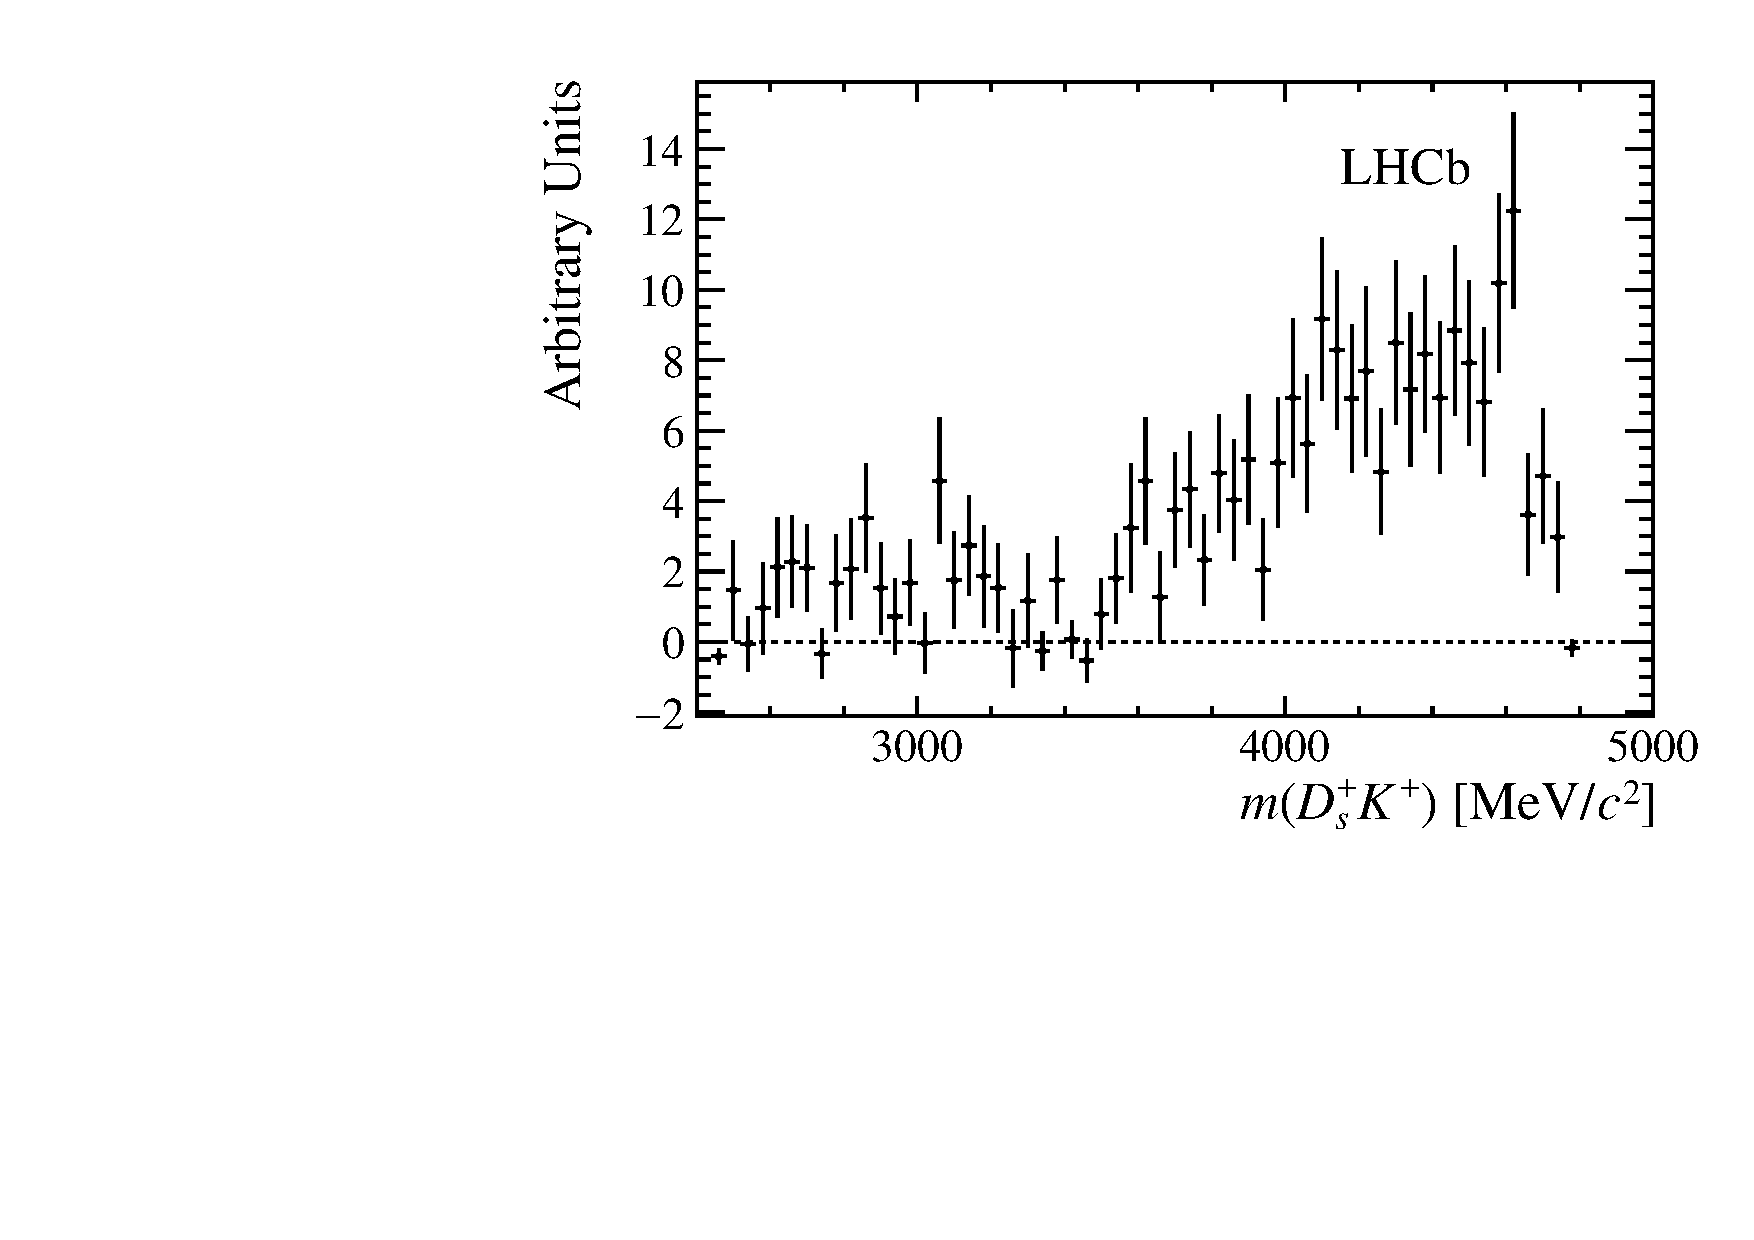
\includegraphics[width=1.0\textwidth]{figs/B2DsKK/DsKp_mass_sweighted.pdf}
    %     %\caption{Normalisation without selection}
    % \end{subfigure}
    \begin{subfigure}[t]{0.49\textwidth}
        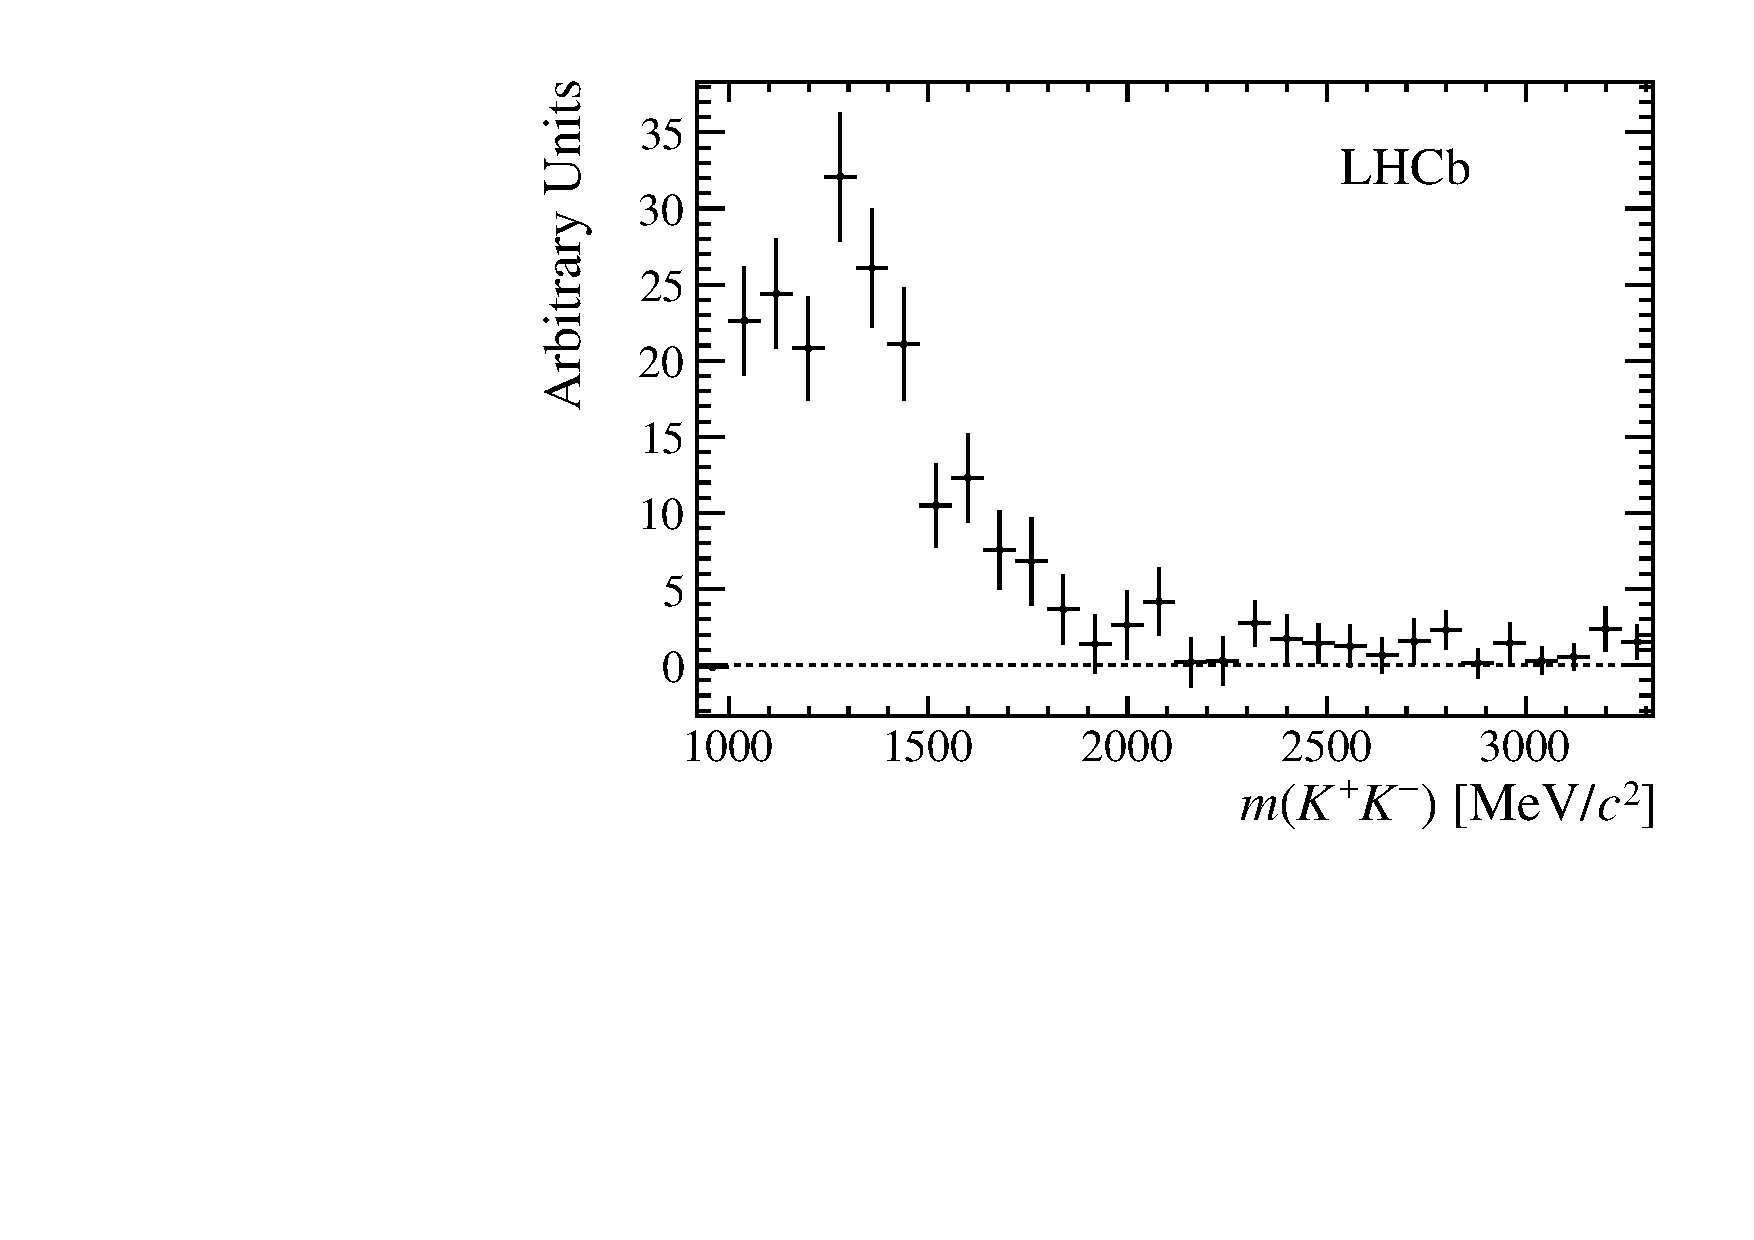
\includegraphics[width=1.0\textwidth]{figs/B2DsKK/phi_mass_sweighted.pdf}
        %\caption{Normalisation without selection}
    \end{subfigure}
    \caption{Two-body mass projections of the background-subtracted efficiency-corrected \decay{\Bp}{\Dsp\Kp\Km} candidates.}
    \label{fig:B2DsKK_twobodyprojections}
\end{figure}
%%%%%%%%%%%%%%%%%%%%%%%%%%%%%%%%%%%%%%%%%%%%%%%%%%%%%%%%%%

The two-body projections $m(D_{s}^{+}K^{-})$ and $m(K^{+}K^{-})$ are obtained for the signal component using the \sPlot technique, shown in Fig.~\ref{fig:B2DsKK_twobodyprojections}. A broad distribution of candidates is found in the region up to $m(\Kp\Km) \simeq 1900 \mevcc$. These plots have been corrected to account for the variation in the relative efficiencies as a function of the phase-space.



Additionally, the distribution of background-subtracted efficiency-corrected \decay{\Bp}{\Dsp\Kp\Km} decays are shown as a function of the two-dimensional space $m^{2}(\Dsp\Km)$ vs. $m^{2}(\Kp\Km)$ in Fig.~\ref{fig:B2DsKK_Dalitzplot}. The candidates can be seen to be localised to a small area of the phase-space. 

%%%%%%%%%%%%%%%%%%%%%%%%%%%%%%%%%%%%%%%%%%%%%%%%%%%%%%%%%%
\begin{figure}[!h]
    \centering
    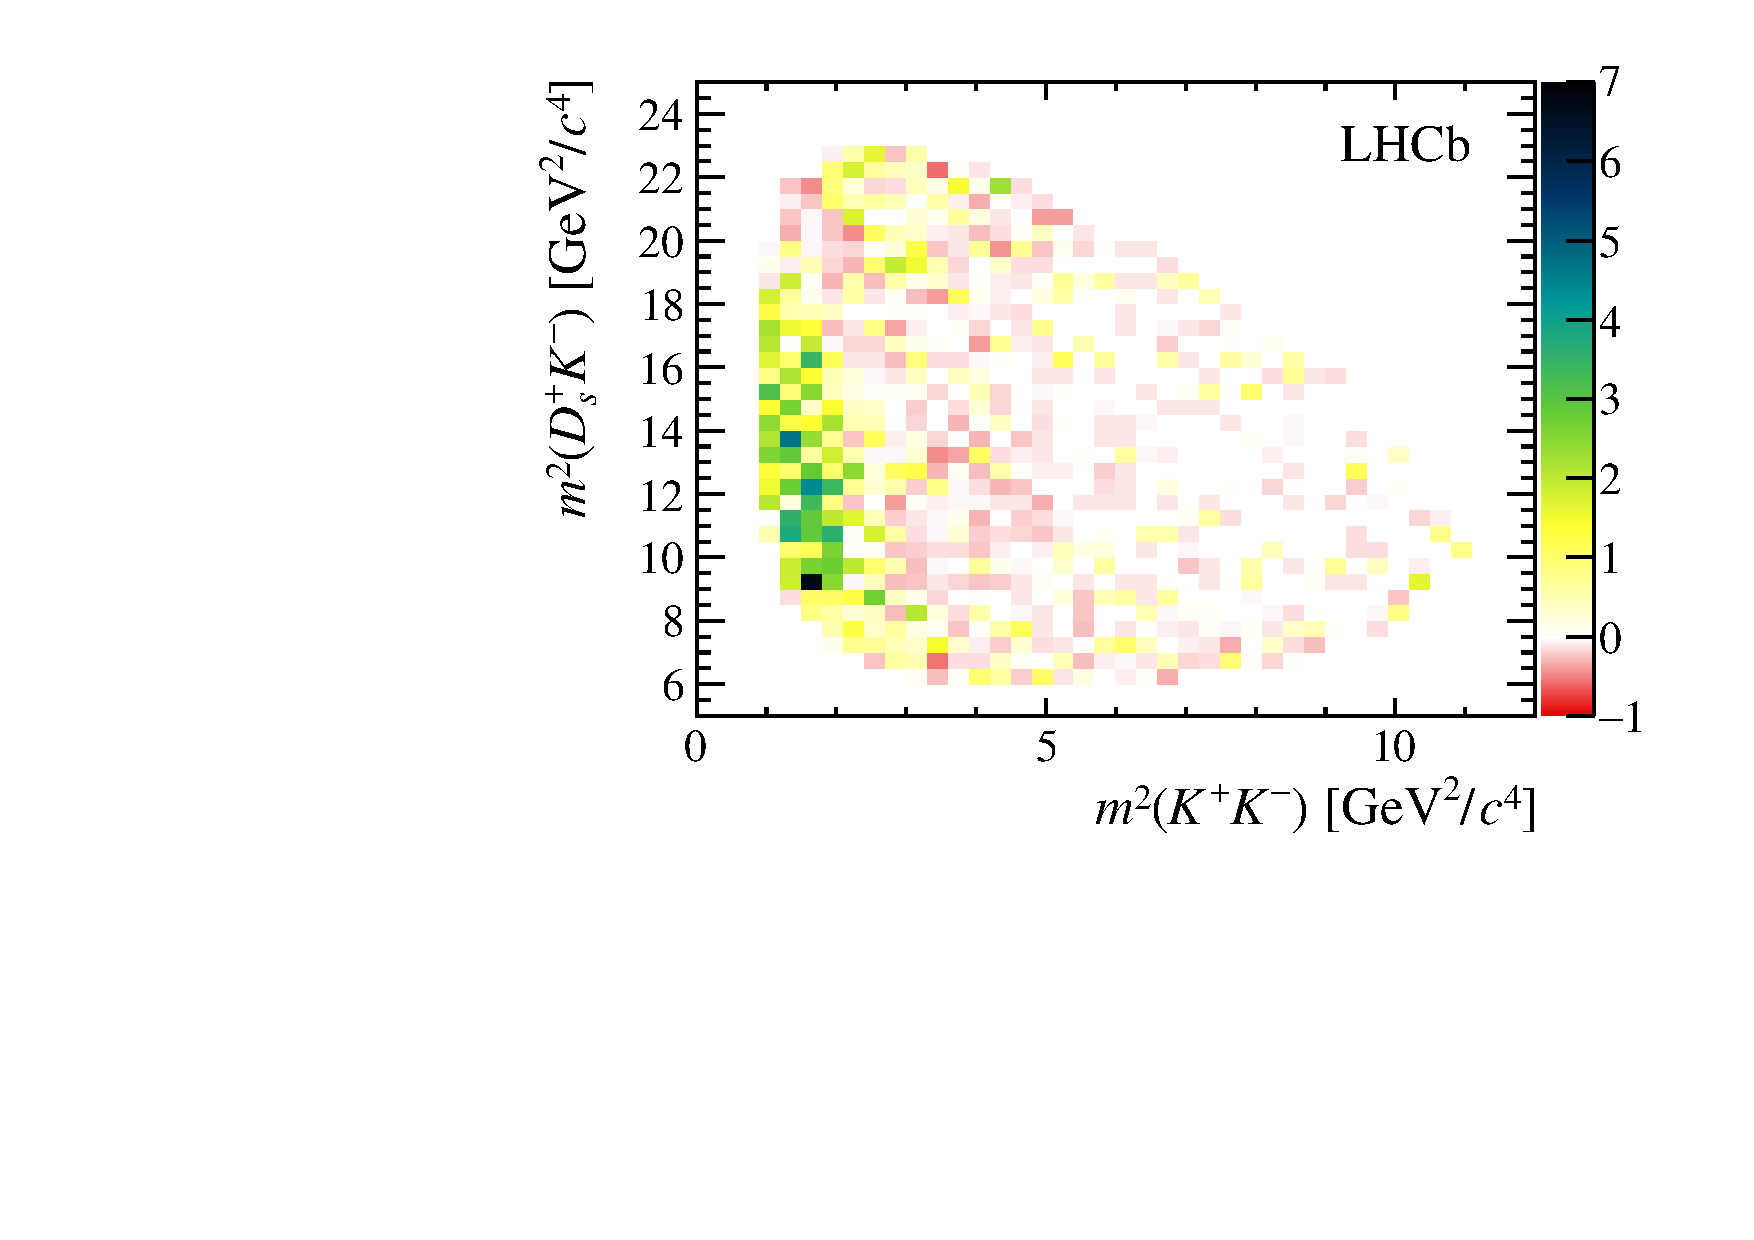
\includegraphics[width=0.7\textwidth]{figs/B2DsKK/Dalitz_plot_sweighted.pdf}
    \caption{The Dalitz plot distribution of background-subtracted efficiency-corrected \decay{\Bp}{\Dsp\Kp\Km} decays.}
    \label{fig:B2DsKK_Dalitzplot}   
\end{figure}
%%%%%%%%%%%%%%%%%%%%%%%%%%%%%%%%%%%%%%%%%%%%%%%%%%%%%%%%%%



The background-subtracted distribution of the angle, $\cos{\theta_{K}}$, defined to be the angle between the direction of the \Kp meson and \Bp momentum vector in the \Kp\Km rest frame is shown in Fig.~\ref{fig:B2DsKK_helicty_angle_bins} in bins of $m(\Kp\Km)$. The distribution of this angle can change depending of the spin of the \Kp\Km system and therefore may help identify the contributing processes. 
% Additionally, the distribution of the angle $\theta_{K}$ is plotted in bins of $m(\Kp\Km)$ in .
% The distribution is observed to change as a function of $m(\Kp\Km)$, which may be a result of interference between competing processes.
% %%%%%%%%%%%%%%%%%%%%%%%%%%%%%%%%%%%%%%%%%%%%%%%%%%%%%%%%%%
% \begin{figure}[!h]
%     \centering
%     \begin{subfigure}[t]{0.59\textwidth}
%         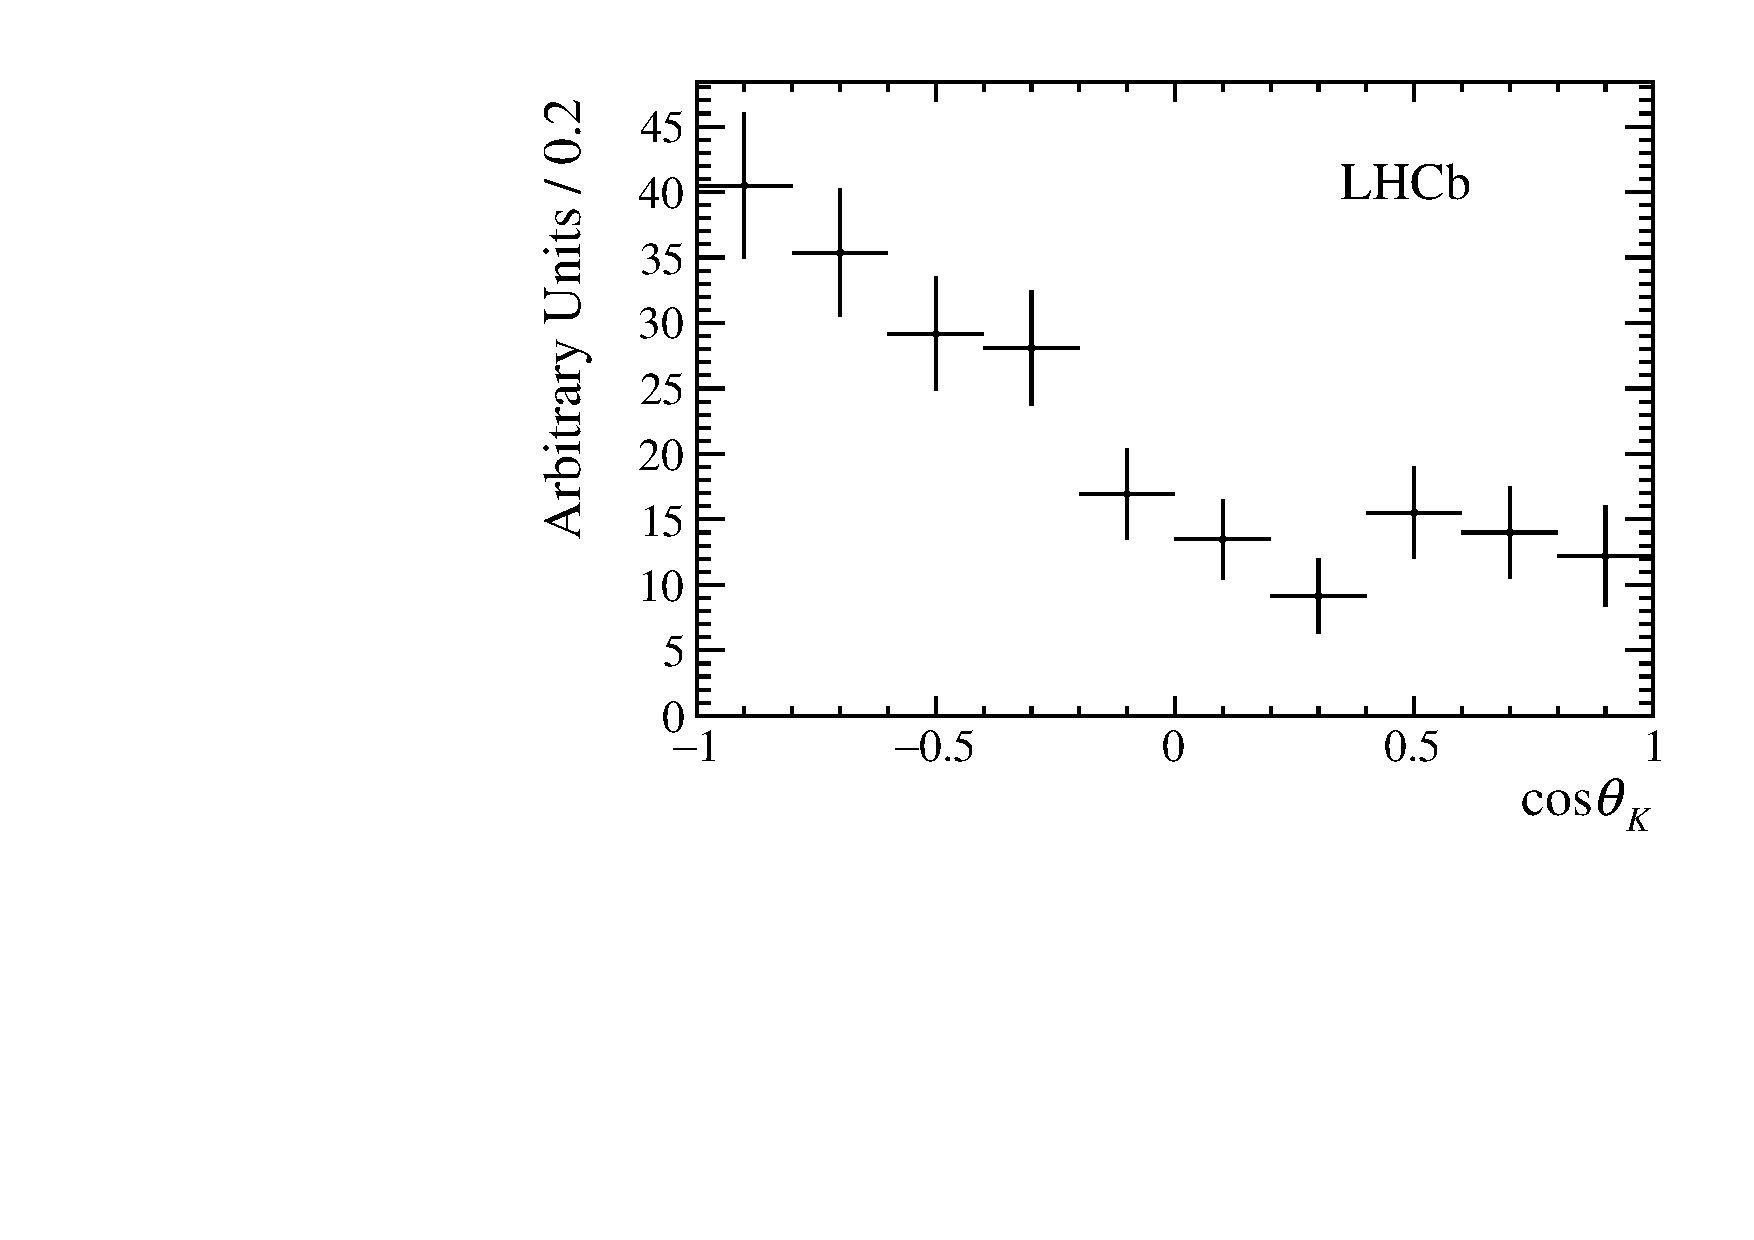
\includegraphics[width=1.0\textwidth]{figs/B2DsKK/helAngle_sweighted.pdf}
%         %\caption{Normalisation without selection}
%     \end{subfigure}
%     \caption{The background-subtracted efficiency-corrected distribution of $\cos{\theta_{K}}$ for \decay{\Bp}{\Dsp\Kp\Km} candidates.}
%     \label{fig:B2DsKK_helicity_angle}
% \end{figure}
% %%%%%%%%%%%%%%%%%%%%%%%%%%%%%%%%%%%%%%%%%%%%%%%%%%%%%%%%%%
%%%%%%%%%%%%%%%%%%%%%%%%%%%%%%%%%%%%%%%%%%%%%%%%%%%%%%%%%%
\begin{figure}[!h]
    \centering
    \begin{subfigure}[t]{0.49\textwidth}
        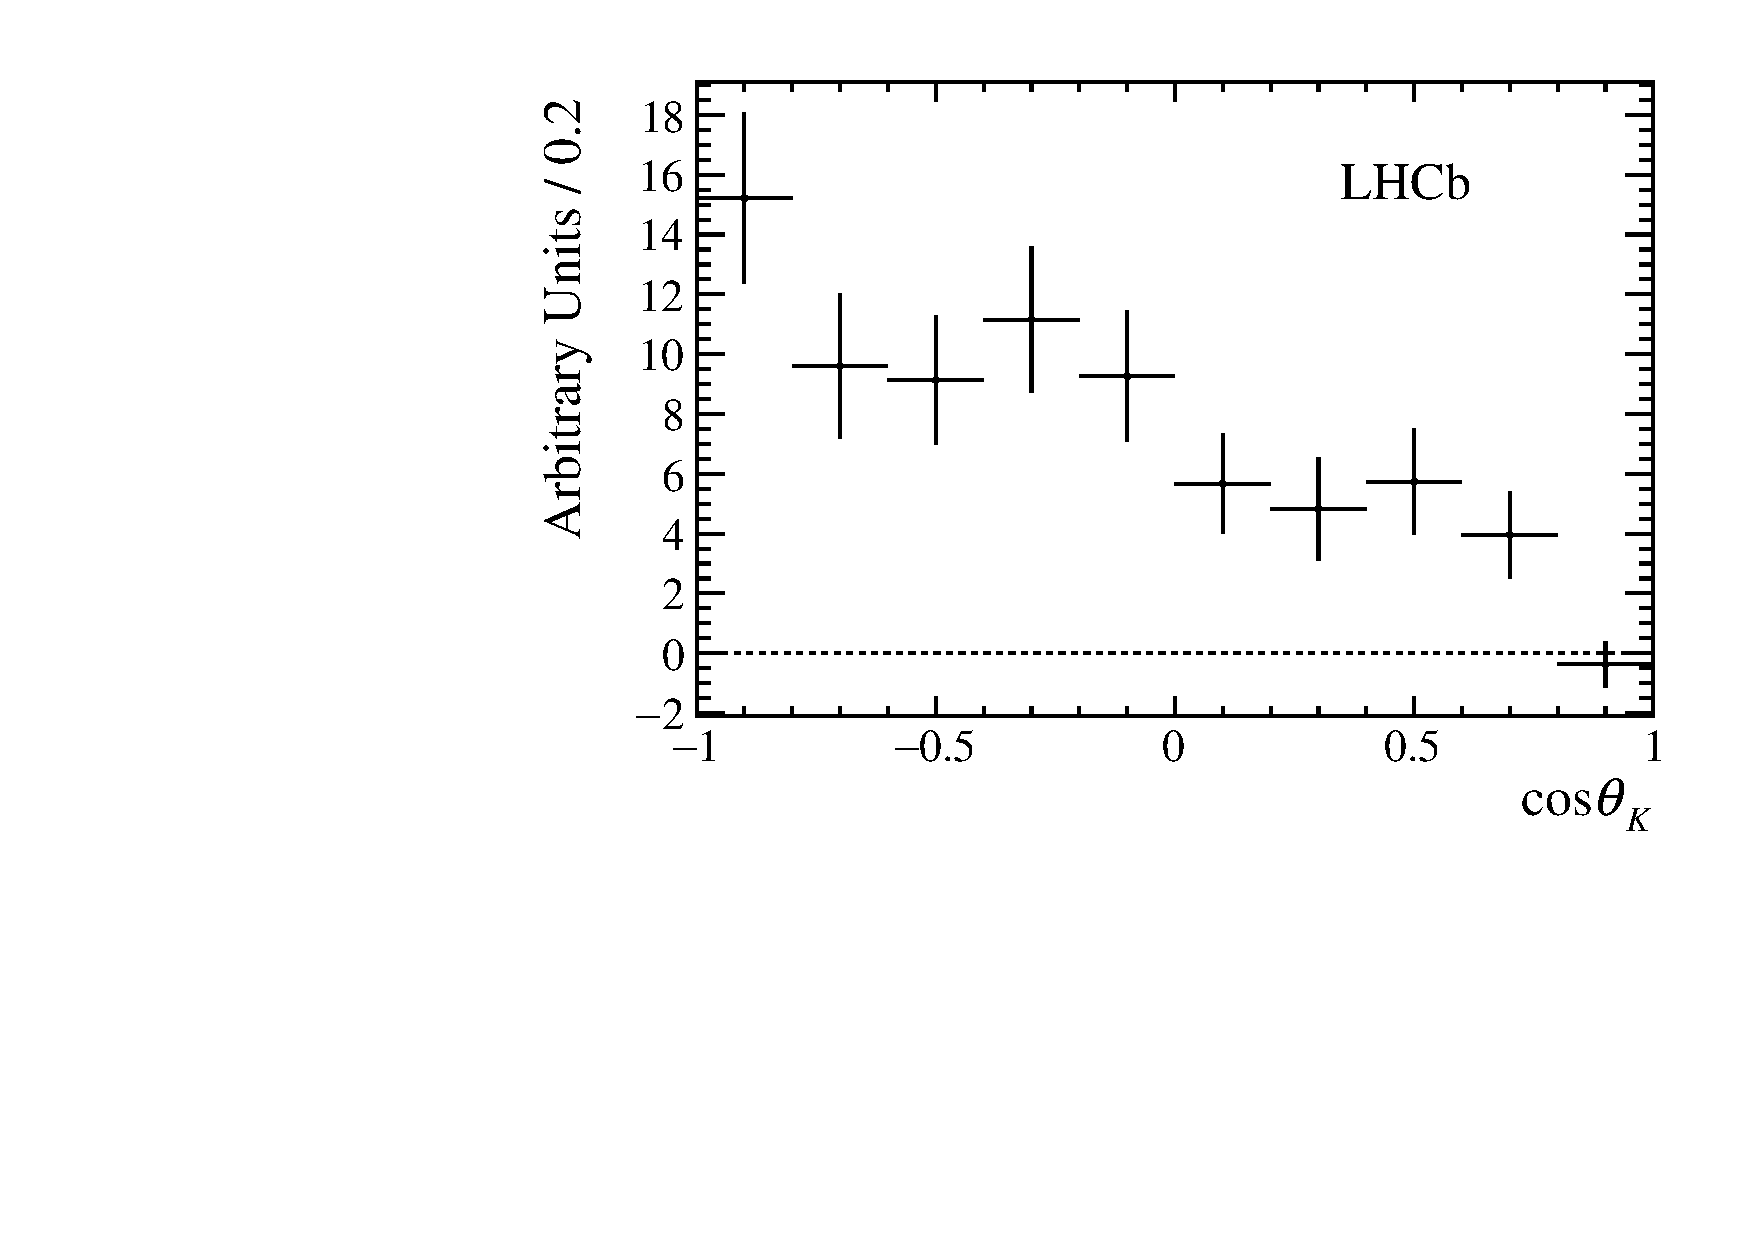
\includegraphics[width=1.0\textwidth]{figs/B2DsKK/helAngle_bin1_sweighted.pdf}
        \caption{$m(\Kp\Km)<1250\mevcc$}
    \end{subfigure}
    \begin{subfigure}[t]{0.49\textwidth}
        \includegraphics[width=1.0\textwidth]{figs/B2DsKK/helAngle_bin2_sweighted.pdf}
        \caption{$1250<m(\Kp\Km)<1500\mevcc$}
    \end{subfigure}
    \begin{subfigure}[t]{0.49\textwidth}
        \includegraphics[width=1.0\textwidth]{figs/B2DsKK/helAngle_bin3_sweighted.pdf}
        \caption{$1500<m(\Kp\Km)<1750\mevcc$}
    \end{subfigure}
    \begin{subfigure}[t]{0.49\textwidth}
        \includegraphics[width=1.0\textwidth]{figs/B2DsKK/helAngle_bin4_sweighted.pdf}
        \caption{$m(\Kp\Km)>1750\mevcc$}
    \end{subfigure}
    \caption{The distribution of $\cos{\theta_{K}}$ in bins of $m(\Kp\Km)$ mass.}
    \label{fig:B2DsKK_helicty_angle_bins}
\end{figure}
%%%%%%%%%%%%%%%%%%%%%%%%%%%%%%%%%%%%%%%%%%%%%%%%%%%%%%%%%%
The distribution of $\cos{\theta_{K}}$ in the region $1500<m(\Kp\Km)<1750\mevcc$ appears to have distinct minimum around $\cos{\theta_{K}}=0$. This may imply a spin-1 resonance contributes in this invariant mass region, for example the $\phiz(1680)$ or $\rho(1700)$ resonances.


%%%%%%%%%%%%%%====================


\subsection{Possible resonant contributions}
\label{sec:B2DsKK_possible_res}

In the search for \decay{\Bp}{\Dsp\phiz} decays, detailed in Chapter~\ref{ch:B2DsPhi}, it is important to understand the contribution from \decay{\Bp}{\Dsp\Kp\Km} decays in the vicinity of the \phiz-meson mass.
A number of possible contributions around this region are investigated using the \laurapp package~\cite{1711.09854}. Simulation samples are generated for different intermediate resonance models.
%To determine similar fractions for \decay{\Bp}{\Dsp\Kp\Km} decays the \laurapp package~\cite{1711.09854} is used to generate a number of simulation samples for different intermediate resonance models.
Only resonances in the \Kp\Km system are considered as no significant structure is observed in the $m(\Dsp\Km)$ distribution in Fig.~\ref{fig:B2DsKK_twobodyprojections}. As such, all resonances are neutral mesons. The resonances, listed in Table~\ref{tab:B2DsKK_models}, are generated separately, therefore the effect of interference between any combination of states has been entirely neglected.    
%The generated samples are described in the following sections.


% \subsubsection{The $\phi(1020)$ resonance} 
% Decays proceeding via a $\phiz(1020)$ are produced as a crosscheck. As the simulations generated with \laurapp have not been reconstructed with the full \lhcb detector model, this sample is compared to the existing full simulation samples. The differences in between the $m(\Kp\Km)$ and $\cos\theta_{K}$ distribution in the two samples are taken as a proxy for the potential level of bias introduced by using these generator level samples instead of full simulation. The distribution of these simulated decays in $m(\Kp\Km)$ and $\cos\theta_{K}$ are shown in Fig.~\ref{fig:DsKK_model_phi1020}. This figure also include the Dalitz plot distribution of the decays parametrised with the variables $m^{2}(\Dsp\Km)$ and $m^{2}(\Kp\Km)$.
% This resonance is generated with a Relativistic Breit-Wigner line shape~\cite{RelBWPhysRev.49.519}.
% %%%%%%%%%%%%%
% \begin{figure}[!h]
%    \centering   
%    \includegraphics[width=0.32\textwidth]{figs/B2DsPhi/phi_phi_mass.pdf}
%    \includegraphics[width=0.32\textwidth]{figs/B2DsPhi/phi_Helicity.pdf}
%    \includegraphics[width=0.32\textwidth]{figs/B2DsPhi/phi_Dalitz_plot.pdf}
%    \caption{The distribution of $m(\Kp\Km)$ (left) the helicity angle $\cos\theta_{K}$ (middle) and Dalitz plot (right) generated for the $\phiz(1020)$ resonance.} 
%    \label{fig:DsKK_model_phi1020}   
% \end{figure}
% %%%%%%%%%%%%%

% \subsubsection{Non-resonant decays}

% In addition to \Kp\Km resonances, a non-resonant model is considered. This model is defined to have a uniform amplitude across the allowed phase-space. The distribution in $m(\Kp\Km)$ of \decay{\Bp}{\Dsp\Kp\Km} decays in Fig.~\ref{fig:B2DsKK_twobodyprojections} is not consistent with this model as there are no candidates above $m(\Kp\Km) \sim 1900\mevcc$. However, this component is included in this study for comparative purposes. The distributions of decays generated with this flat model are shown in Fig.~\ref{fig:DsKK_model_NR}. 

% %%%%%%%%%%%%%
% \begin{figure}[!h]
%    \centering   
%    \includegraphics[width=0.32\textwidth]{figs/B2DsPhi/NR_phi_mass.pdf}
%    \includegraphics[width=0.32\textwidth]{figs/B2DsPhi/NR_Helicity.pdf}
%    \includegraphics[width=0.32\textwidth]{figs/B2DsPhi/NR_Dalitz_plot.pdf}
%    \caption{The distribution of $m(\Kp\Km)$ (left) the helicity angle $\cos\theta_{K}$ (middle) and Dalitz plot (right) generated for non-resonant decays.} 
%    \label{fig:DsKK_model_NR}   
% \end{figure}
% %%%%%%%%%%%%%

% \subsubsection{The $f_{0}^{0}(980)$ resonance}

% The $f_{0}^{0}(980)$ resonance is a light unflavoured $J^{P} = 0^{+}$ state with mass $990\pm20\mevcc$ and width 10--100\mevcc~\cite{PDG2016}. It has been observed to decay to $\Kp\Km$ making it a suitable resonance to consider. Although it's mass is at the lower end of the range considered here, it's significant width allows it to contribute at higher invariant masses. This component is modelled with the Flatt\'{e} line shape~\cite{Flatte:1976xu} and the relevant distributions shown in Fig.~\ref{fig:DsKK_model_f0980}.
% %%%%%%%%%%%%%
% \begin{figure}[!h]
%    \centering   
%    \includegraphics[width=0.32\textwidth]{figs/B2DsPhi/f0_phi_mass.pdf}
%    \includegraphics[width=0.32\textwidth]{figs/B2DsPhi/f0_Helicity.pdf}
%    \includegraphics[width=0.32\textwidth]{figs/B2DsPhi/f0_Dalitz_plot.pdf}
%    \caption{The distribution of $m(\Kp\Km)$ (left) the helicity angle $\cos\theta_{K}$ (middle) and Dalitz plot (right) generated for the $f_{0}^{0}(980)$ resonance.} 
%    \label{fig:DsKK_model_f0980}   
% \end{figure}
% %%%%%%%%%%%%%

% \subsubsection{The $a_{0}^{0}(980)$ resonance}
% The $a_{0}^{0}(980)$ resonance is a light unflavoured $J^{P} = 0^{+}$ state with mass $980\pm20\mevcc$ and width 50--100\mevcc and has been observed to decay to $\PK\Kb$ final states~\cite{PDG2016}. This resonance is also modelled with the Flatt\'{e} line shape and the relevant distributions are shown in Fig~\ref{fig:DsKK_model_a0980}.
% %%%%%%%%%%%%%
% \begin{figure}[!h]
%    \centering   
%    \includegraphics[width=0.32\textwidth]{figs/B2DsPhi/a0_phi_mass.pdf}
%    \includegraphics[width=0.32\textwidth]{figs/B2DsPhi/a0_Helicity.pdf}
%    \includegraphics[width=0.32\textwidth]{figs/B2DsPhi/a0_Dalitz_plot.pdf}
%    \caption{The distribution of $m(\Kp\Km)$ (left) the helicity angle $\cos\theta_{K}$ (middle) and Dalitz plot (right) generated for the $a_{0}^{0}(980)$ resonance.} 
%    \label{fig:DsKK_model_a0980}   
% \end{figure}
% %%%%%%%%%%%%%

% \subsubsection{The $f_{0}^{0}(1370)$ resonance}
% The $f_{0}^{0}(1370)$ resonance is a light unflavoured $J^{P} = 0^{+}$ state with a mass in the range 1200--1500\mevcc and width in the range 200--500\mevcc. It has been observed to decay to the \kaon\Kb final states. It is modelled with a Relativistic Breit-Wigner line shape and the relevant distributions are shown in Fig.~\ref{fig:DsKK_model_f01370}.
% %%%%%%%%%%%%%
% \begin{figure}[!h]
%    \centering   
%    \includegraphics[width=0.32\textwidth]{figs/B2DsPhi/f0_1370_phi_mass.pdf}
%    \includegraphics[width=0.32\textwidth]{figs/B2DsPhi/f0_1370_Helicity.pdf}
%    \includegraphics[width=0.32\textwidth]{figs/B2DsPhi/f0_1370_Dalitz_plot.pdf}
%    \caption{The distribution of $m(\Kp\Km)$ (left) the helicity angle $\cos\theta_{K}$ (middle) and Dalitz plot (right) generated for the $f_{0}^{0}(1370)$ resonance.} 
%    \label{fig:DsKK_model_f01370}   
% \end{figure}
% %%%%%%%%%%%%%

% \subsubsection{The $f_{2}^{0}(1270)$ resonance}
% The $f_{2}^{0}(1270)$ resonance is a $J^{P} = 2^{+}$ state with mass $1275.5\pm08\mevcc$ and width $186.7^{+2.2}_{-2.5}\mevcc$ that has been observed to decay to \kaon\Kb final states. This resonance is modelled with a Relativistic Breit-Wigner line shape as shown in Fig.~\ref{fig:DsKK_model_f21270}.

% %%%%%%%%%%%%%
% \begin{figure}[!h]
%    \centering   
%    \includegraphics[width=0.32\textwidth]{figs/B2DsPhi/f2_phi_mass.pdf}
%    \includegraphics[width=0.32\textwidth]{figs/B2DsPhi/f2_Helicity.pdf}
%    \includegraphics[width=0.32\textwidth]{figs/B2DsPhi/f2_Dalitz_plot.pdf}
%    \caption{The distribution of $m(\Kp\Km)$ (left) the helicity angle $\cos\theta_{K}$ (middle) and Dalitz plot (right) generated for the $f_{2}^{0}(1270)$ resonance.} 
%    \label{fig:DsKK_model_f21270}   
% \end{figure}
% %%%%%%%%%%%%%


% \subsubsection{The $a_{2}^{0}(1320)$ resonance}
% The $a_{2}^{0}(1320)$ resonance is a $J^{P} = 2^{+}$ state with a mass $1318.1\pm0.7\mevcc$ and width $109.8\pm2.4\mevcc$ (both measured in the \kaon\Kb mode) observed decaying to the \kaon\Kb final state. This resonance is modelled with a Relativistic Breit-Wigner line shape and shown in Fig.~\ref{fig:DsKK_model_a21320}.
% %%%%%%%%%%%%%
% \begin{figure}[!h]
%    \centering   
%    \includegraphics[width=0.32\textwidth]{figs/B2DsPhi/a2_1320_phi_mass.pdf}
%    \includegraphics[width=0.32\textwidth]{figs/B2DsPhi/a2_1320_Helicity.pdf}
%    \includegraphics[width=0.32\textwidth]{figs/B2DsPhi/a2_1320_Dalitz_plot.pdf}
%    \caption{The distribution of $m(\Kp\Km)$ (left) the helicity angle $\cos\theta_{K}$ (middle) and Dalitz plot (right) generated for the $a_{2}^{0}(1320)$ resonance.} 
%    \label{fig:DsKK_model_a21320}   
% \end{figure}
% %%%%%%%%%%%%%



%%%%%%%%%%%%%%%%%%%%%%%%%%%%%%%%%%%%%%%%%%%%%%%%%%%%%%%%%%%%%%%%%%%%%%%%%%%%%%
%%%%%%%%%%%%%%%%%%%%%%%%%%%%%%%%%%%%%%%%%%%%%%%%%%%%%%%%%%%%%%%%%%%%%%%%%%%%%%
%S[table-format=4.1(3)]
\begin{table}[h]
    \centering
    \begin{tabular}{ l c c c c c }
        \hline
        Resonance           & $J^{P}$ & Mass (\mevcc)       & Width (\mevcc)        & Line shape    & Observed decay    \\
        \hline
        $\phi(1020)$        & $1^{-}$ & 1019.46$\pm$0.016   & 4.247$\pm$0.016       & RBW           & \Kp\Km            \\
        \hline
        $f_{0}^{0}(980)$    & $0^{+}$ & 990$\pm$20          & 10--100               & Flatt\'{e}    & \Kp\Km            \\
        $a_{0}^{0}(980)$    & $0^{+}$ & 980$\pm$20          & 50--100               & Flatt\'{e}    & \kaon\Kb          \\
        $f_{0}^{0}(1370)$   & $0^{+}$ & 1200--1500          & 200--500              & RBW           & \kaon\Kb          \\
        $f_{2}^{0}(1270)$   & $2^{+}$ & 1275.5$\pm$08       & $186.7^{+2.2}_{-2.5}$ & RBW           & \kaon\Kb          \\
        $a_{2}^{0}(1320)$   & $2^{+}$ & 1318.1$\pm$0.7      & 109.8$\pm$2.4         & RBW           & \kaon\Kb          \\
        \hline
        Non-resonant        & -       &  -              & -                     & -             &                   \\
        \hline
    \end{tabular}  
    \caption{The properties of the resonances that could contribute to \decay{\Bp}{\Dsp\Kp\Km} decays in the vicinity of the \phiz-meson mass decays, from Ref.~\cite{PDG2016}. Resonances are generated using a Relativistic Breit-Wigner (RBW)~\cite{RelBWPhysRev.49.519} or Flatt\'{e}~\cite{Flatte:1976xu} line shape. } 
    \label{tab:B2DsKK_models}
\end{table}


Decays proceeding via a $\phiz(1020)$ are produced as a crosscheck. As the simulations generated with \laurapp have not been reconstructed with the full \lhcb detector model, this sample is compared to the existing full simulation samples. The differences in between the $m(\Kp\Km)$ and $\cos\theta_{K}$ distribution in the two samples are taken as a proxy for the potential level of bias introduced by using these generator level samples instead of full simulation. 

The distribution of the models listed in Table~\ref{tab:B2DsKK_models} in $m(\Kp\Km)$, $\cos\theta_{K}$ and the \decay{\Bp}{\Dsp\Kp\Km} Dalitz plot are shown in Figs.~\ref{fig:B2DsKK_models_1} and~\ref{fig:B2DsKK_models_2}. 
%This figure also include the Dalitz plot distribution of the decays parametrised with the variables $m^{2}(\Dsp\Km)$ and $m^{2}(\Kp\Km)$.
In addition to \Kp\Km resonances, a non-resonant model is considered. This model is defined to have a uniform amplitude across the allowed phase-space. The distribution in $m(\Kp\Km)$ of \decay{\Bp}{\Dsp\Kp\Km} decays in Fig.~\ref{fig:B2DsKK_twobodyprojections} is not consistent with this model as there are no candidates above $m(\Kp\Km) \sim 1900\mevcc$. However, this component is included in this study for comparative purposes. 
%The distributions of decays generated with this flat model are shown in Fig.~\ref{fig:B2DsKK_model_NR}. 



%%%%%%%%%%%%%%%%%%%%%%%%%%%%%%%%%%%%%%%%%%%%%%%%%%%%%%%%%%
\begin{figure}[!h]
    \centering
    \begin{subfigure}[t]{1.0\textwidth}
       \includegraphics[width=0.32\textwidth]{figs/B2DsPhi/phi_phi_mass.pdf}
       \includegraphics[width=0.32\textwidth]{figs/B2DsPhi/phi_Helicity.pdf}
       \includegraphics[width=0.32\textwidth]{figs/B2DsPhi/phi_Dalitz_plot.pdf}
       \caption{$\phiz(1020)$} 
       \label{fig:B2DsKK_model_phi}
    \end{subfigure}
    \begin{subfigure}[t]{1.0\textwidth}
        \includegraphics[width=0.32\textwidth]{figs/B2DsPhi/NR_phi_mass.pdf}
        \includegraphics[width=0.32\textwidth]{figs/B2DsPhi/NR_Helicity.pdf}
        \includegraphics[width=0.32\textwidth]{figs/B2DsPhi/NR_Dalitz_plot.pdf}
        \caption{Non-resonant} 
       \label{fig:B2DsKK_model_NR}
    \end{subfigure}
    \begin{subfigure}[t]{1.0\textwidth}
        \includegraphics[width=0.32\textwidth]{figs/B2DsPhi/f0_phi_mass.pdf}
        \includegraphics[width=0.32\textwidth]{figs/B2DsPhi/f0_Helicity.pdf}
        \includegraphics[width=0.32\textwidth]{figs/B2DsPhi/f0_Dalitz_plot.pdf}
        \caption{$f_{0}^{0}(980)$} 
    \end{subfigure}
    \begin{subfigure}[t]{1.0\textwidth}
        \includegraphics[width=0.32\textwidth]{figs/B2DsPhi/a0_phi_mass.pdf}
        \includegraphics[width=0.32\textwidth]{figs/B2DsPhi/a0_Helicity.pdf}
        \includegraphics[width=0.32\textwidth]{figs/B2DsPhi/a0_Dalitz_plot.pdf}
        \caption{$a_{0}^{0}(980)$} 
    \end{subfigure}
    \caption{The distribution of $m(\Kp\Km)$ (left) the helicity angle $\cos\theta_{K}$ (middle) and Dalitz plot (right) generated for the various models.}
    \label{fig:B2DsKK_models_1}
\end{figure}
%%%%%%%%%%%%%%%%%%%%%%%%%%%%%%%%%%%%%%%%%%%%%%%%%%%%%%%%%%
%%%%%%%%%%%%%%%%%%%%%%%%%%%%%%%%%%%%%%%%%%%%%%%%%%%%%%%%%%
\begin{figure}[!h]
    \centering
    \begin{subfigure}[t]{1.0\textwidth}
        \includegraphics[width=0.32\textwidth]{figs/B2DsPhi/f0_1370_phi_mass.pdf}
        \includegraphics[width=0.32\textwidth]{figs/B2DsPhi/f0_1370_Helicity.pdf}
        \includegraphics[width=0.32\textwidth]{figs/B2DsPhi/f0_1370_Dalitz_plot.pdf}
        \caption{$f_{0}^{0}(1370)$}
    \end{subfigure}
    \begin{subfigure}[t]{1.0\textwidth}
        \includegraphics[width=0.32\textwidth]{figs/B2DsPhi/f2_phi_mass.pdf}
        \includegraphics[width=0.32\textwidth]{figs/B2DsPhi/f2_Helicity.pdf}
        \includegraphics[width=0.32\textwidth]{figs/B2DsPhi/f2_Dalitz_plot.pdf}
        \caption{$f_{2}^{0}(1270)$} 
    \end{subfigure}
    \begin{subfigure}[t]{1.0\textwidth}
        \includegraphics[width=0.32\textwidth]{figs/B2DsPhi/a2_1320_phi_mass.pdf}
        \includegraphics[width=0.32\textwidth]{figs/B2DsPhi/a2_1320_Helicity.pdf}
        \includegraphics[width=0.32\textwidth]{figs/B2DsPhi/a2_1320_Dalitz_plot.pdf}
        \caption{$a_{2}^{0}(1320)$} 
    \end{subfigure}
    \caption{The distribution of $m(\Kp\Km)$ (left) the helicity angle $\cos\theta_{K}$ (middle) and Dalitz plot (right) generated for the various models.}
    \label{fig:B2DsKK_models_2}
\end{figure}
%%%%%%%%%%%%%%%%%%%%%%%%%%%%%%%%%%%%%%%%%%%%%%%%%%%%%%%%%%






%In order to choose suitable fractions for the \decay{\Bp}{\Dsp\Kp\Km} fit component a number of points are considered;
\subsubsection{Models consistent with data}

To determine which of the models that contribute in the region of the \phiz-meson mass are most consistent with the observed signal, the following points are considered: 

\begin{itemize}
\item Very few events are observed above 2000\mevcc in the background-subtracted $m(\Kp\Km)$ distribution, therefore the non-resonant model is neglected.
\item No significant peaking structure is observed in the $m(\Kp\Km)$ spectrum so on-shell resonances are neglected
\item The helicity distribution at low $m(\Kp\Km)$ shows no distinctive structure so spin zero states are favoured.  
\item As this is not a full amplitude analysis no attempt is made to include the effects of interference, either between the remaining off-shell resonances or between these and any possible \decay{\Bp}{\Dsp\phiz} decays.
\end{itemize}

These considerations leave the $f_{0}^{0}(980)$ and $a_{0}^{0}(980)$ resonances as possible contributions in the region of the \phiz-meson mass. 

%%%%%%%%%%%%%%====================


\subsubsection{Looking forward}

This analysis provides an initial insight to the possible processes that might contribute to the \decay{\Bp}{\Dsp\Kp\Km} decay. However, a full amplitude analysis is needed to understand the competing decays and interference between the amplitudes. This search contains only a fraction of the Run II data sample; the inclusion of the 2017 and 2018 samples would provide a statistically solid base to further this line of investigation. 

